%%%%%%%%%%%%%%%%%%%%%%%%%%%%%%%%%%%%%%%%%%%%%%%%%%%%%%%%%%%%%%%%%

\documentclass[12pt,english]{article}
\usepackage{mathpazo}
\renewcommand{\sfdefault}{lmss}
\renewcommand{\ttdefault}{lmtt}
\usepackage{geometry}
\geometry{verbose, tmargin=1.14in, bmargin=1.14in, lmargin=1.4in, rmargin=1.4in}
\usepackage{color}
\usepackage{etoolbox}
\usepackage[american]{babel}
\usepackage[hang,flushmargin]{footmisc}
\usepackage{float}
\usepackage{booktabs}
\newsavebox{\tablebox}
\usepackage{placeins}
\usepackage{color}
\usepackage{titletoc}
\usepackage{mathptmx}
\usepackage{bm}
\usepackage{graphicx}
\usepackage{setspace}
\usepackage[compact]{titlesec}
    \titlespacing*{\section}{0pt}{.5ex}{1ex}
    \titlespacing*{\subsection}{0pt}{.5ex}{1ex}
    \titlespacing*{\subsubsection}{0pt}{0.5ex}{0ex}
\renewcommand{\footnotesize}{\fontsize{9pt}{11pt}\selectfont}\usepackage[unicode=true,
 bookmarks=true,bookmarksnumbered=false,bookmarksopen=false,
 breaklinks=false,pdfborder={0 0 0},pdfborderstyle={},backref=false,colorlinks=true]
 {hyperref}
\hypersetup{
 linkcolor=[rgb]{0,0,0.6}, citecolor=[rgb]{0,0,0.6}, urlcolor=[rgb]{0,0,0.6}}
\usepackage{breakurl}
\usepackage{atbegshi}
\AtBeginDocument{\AtBeginShipoutNext{\AtBeginShipoutDiscard}}
\usepackage{scalerel,stackengine}
\stackMath
\newcommand\reallywidehat[1]{%
\savestack{\tmpbox}{\stretchto{%
  \scaleto{%
    \scalerel*[\widthof{\ensuremath{#1}}]{\kern-.6pt\bigwedge\kern-.6pt}%
    {\rule[-\textheight/2]{1ex}{\textheight}}%WIDTH-LIMITED BIG WEDGE
  }{\textheight}% 
}{0.5ex}}%
\stackon[1pt]{#1}{\tmpbox}%
}
\makeatletter
\usepackage{csvsimple}

%%%%%%%%%%%%%%%%%%%%%%%%%%%%%%%%%%%%%%%%%%%%%%%%%%%%%%%%%%%%%%%%%

\providecommand{\tabularnewline}{\\}

%%%%%%%%%%%%%%%%%%%%%%%%%%%%%%%%%%%%%%%%%%%%%%%%%%%%%%%%%%%%%%%%%

\usepackage{multirow}
\usepackage{tikz}
\usetikzlibrary{positioning}
\usetikzlibrary{patterns,decorations.pathreplacing}
\usepackage[font={bf,sc}]{caption}
\usetikzlibrary{arrows}
\usepackage{rotating}
\usepackage{pdflscape}
\usepackage{makecell}
\usepackage{pdflscape}
\usepackage{booktabs}
\usepackage{tabularx}
\usepackage{geometry}
\usepackage{natbib}
\usepackage{amsmath}
\usepackage{threeparttable}
\DeclareSymbolFont{operators} {OT1}{lmr} {m}{n}
\DeclareSymbolFont{letters} {OML}{cmm} {m}{it}
\DeclareSymbolFont{symbols} {OMS}{cmsy}{m}{n}
\SetSymbolFont{operators}{bold}{OT1}{cmr}{b}{n}
\SetSymbolFont{letters}{bold}{OML}{cmm}{b}{it}
\SetSymbolFont{symbols}{bold}{OMS}{cmsy}{b}{n}
\newcolumntype{Y}{>{\centering\arraybackslash}X}
\newcommand{\cmmnt}[1]{\ignorespaces}
\AtBeginDocument{
  \def\labelitemii{\(\ast\)}
  \def\labelitemiii{\(\star\)}
}
\usepackage{multicol}
\usepackage{etoolbox}
\usepackage{relsize}
\setlength{\columnsep}{1cm} 
\patchcmd{\thebibliography}
  {\list}
  {\begin{multicols}{2}\smaller\list}
  {}
  {}
\appto{\endthebibliography}{\end{multicols}}
\usepackage{pgfplots}
\pgfmathdeclarefunction{gauss}{2}{%
  \pgfmathparse{1/(#2*sqrt(2*pi))*exp(-((x-#1)^2)/(2*#2^2))}%
}
\makeatletter
\newcommand{\lyxdot}{.}
\newcommand*{\centerfloat}{%
  \parindent \z@
  \leftskip \z@ \@plus 1fil \@minus \textwidth
  \rightskip\leftskip
  \parfillskip \z@skip}
\makeatother
\usepackage{titlesec}
\makeatletter
\titleformat{\section}[runin]{}{}{0pt}{\@gobble}
\titleformat{\subsection}[runin]{}{}{0pt}{\@gobble}
\titleformat{\subsubsection}[runin]{}{}{0pt}{\@gobble}
\makeatother
\titlespacing{\section}{\parindent}{0pt}{0pt}
\titlespacing{\subsection}{\parindent}{0pt}{0pt}
\titlespacing{\subsubsection}{\parindent}{0pt}{0pt}

%%%%%%%%%%%%%%%%%%%%%%%%%%%%%%%%%%%%%%%%%%%%%%%%%%%%%%%%%%%%%%%%%

\begin{document}

%%%%%%%%%%%%%%%%%%%%%%%%%%%%%%%%%%%%%%%%%%%%%%%%%%%%%%%%%%%%%%%%%

\sloppy

\title{\textcolor{black}{\textsc{Tables and Figures \\\ for \\\ Local Elites as State Capacity}:}\\
\textcolor{black}{\textsc{\Large{How City Chiefs Use Local Information to Increase Tax Compliance in the D.R. Congo}}}
\textcolor{black}{\textbf{\Huge{}}}
}\thanks{\scriptsize{AEA RCT Registry ID: AEARCTR-0003308.}}

\author{By Pablo Bal\'an, Augustin Bergeron, Gabriel Tourek, \\ and Jonathan L. Weigel\thanks{\scriptsize Affiliations: Harvard University (pbalan@g.harvard.edu), Harvard University (augustinbergeron@fas.harvard.edu), MIT (gztourek@mit.edu), Haas School of Business, University of California Berkeley and CEPR (jweigel@berkeley.edu).}}

\maketitle

\addtocounter{page}{-2}

\singlespacing


%%%%%%%%%%%%%%%%%%%%%%%%%%%%%%%%%%%%%%%%%%%%%%%%%%%%%%%%%%%%%%%%%
 
\thispagestyle{empty}
 
 %%%%%%%%%%%%%%%%%%%%%%%%%%%%%%%%%%%%%%%%%%%%%%%%%%%%%%%%%%%%%%%%%
 
\newgeometry{verbose, tmargin=1in, bmargin=1in, lmargin=1.2in, rmargin=1.2in}

\onehalfspacing
\normalsize

\section{Main Tables and Figures}

\begin{table}[ht]
\textbf{\caption{\label{table_activities} Components of the Tax Campaign and its Evaluation}} 
\centering
\centerfloat
\begin{lrbox}{\tablebox}
\begin{tabular}{rlcccc}
  \hline
    \hline
    \\
& \textbf{Activity} & \textbf{Actor} & \textbf{Timing} & \textbf{N} & \textbf{J} \\ 
  \hline
  \\
& \textbf{Tax campaign} \\
& Property registration  &   Collectors & May-Dec 2018 & 45,162  & 356   \\ 
      & Tax visits & Collectors & May-Dec 2018  & 45,162  & 356 \\ 
      \\
 &      \textbf{Evaluation} \\
& Baseline survey &   Enumerators & Jul-Dec 2017 & 4,246 & 356 \\ 
   & Midline survey &  Enumerators & Jun 2018-Feb 2019 & 36,130 & 356 \\ 
   & Endline  survey &  Enumerators & Mar-Sep 2019 & 3,893 & 356 \\ 
\hline
\end{tabular}
\end{lrbox}
\usebox{\tablebox}\\[1ex]
\parbox{6in}{\footnotesize \textit{Notes}: N = number of observations, J = number of clusters (neighborhoods). The property register has more observations per neighborhood than the midline survey because the former includes information on all compounds, including (exempt) government buildings, churches, and empty lots, while the midline survey was only conducted with privately owned plots liable for the property tax. The primary tax outcomes result from merging official property tax records with data from the property register. The mechanics of the tax campaign and data sources are discussed, respectively, in Sections \ref{mechanics} and \ref{data}.} 
\end{table}

%%%%%%%%%%%%%%%%%%%%%%%%%%%%%%%%%%%%%%%%%%%%%%%%%%%%%%%%%%%%%%%%%

\begin{table}[H]
\centering{}\caption{Treatment Allocation}
\label{tab:tmt} %
\centerfloat
\begin{lrbox}{\tablebox}
\begin{tabular}{lccccc}
  \hline
    \hline
    \\
\textbf{Treatment}  & \textbf{Central}  & \textbf{Local}  & \textbf{CLI}  & \textbf{CXL}  & \textbf{Control} \tabularnewline
\midrule 
Neighborhoods  & 110  & 111  & 80  & 50  & 5 \tabularnewline
Properties  & 14,489  & 14,383  & 9,422 & 6,071  & 797 \tabularnewline
\hline
\end{tabular}
\end{lrbox}
\usebox{\tablebox}\\[1ex]
\parbox{6in}{\footnotesize \textit{Notes}: This table shows the numbers of neighborhoods (clusters) and properties assigned to each treatment arm. In Central, state agents hired by the provincial tax ministry collected property taxes, while in Local, neighborhood chiefs collected. CLI is short for Central + Local Information, a treatment arm in which tax ministry agents consulted with chiefs before making tax visits. In CXL, or Central X Local, one agent of the tax ministry and one chief worked together on the campaign. In Control, citizens received tax letters informing them of their responsibility to pay at the tax ministry (rather than paying to collectors), as was the status quo declarative system in Kananga until 2016. We discuss these treatments in Section \ref{treatment_arms}. We also discuss the reason for differential allocation of clusters across treatment arms in Section \ref{different_allocation}.}
\end{table}

%%%%%%%%%%%%%%%%%%%%%%%%%%%%%%%%%%%%%%%%%%%%%%%%%%%%%%%%%%%%%%%%%

\clearpage

%%%%%%%%%%%%%%%%%%%%%%%%%%%%%%%%%%%%%%%%%%%%%%%%%%%%%%%%%%%%%%%%%

\begin{table}[H]
\vspace*{-1cm}
\textbf{\caption{Randomization Balance}\label{tab:balance_tests}}
\centering
\tiny{\csvautotabular[respect underscore=true]{Output/main_balance_baseline.csv}}
\\
\tiny{\csvautotabular[respect underscore=true]{Output/main_balance_midline.csv}}
\normalsize{{
\def\sym#1{\ifmmode^{#1}\else\(^{#1}\)\fi}
\begin{tabular}{l*{3}{c}}
\hline\hline
                &\multicolumn{1}{c}{Baseline to Endline Attrition}&\multicolumn{1}{c}{Baseline Replacement}&\multicolumn{1}{c}{Midline Attrition}\\
                &\multicolumn{1}{c}{(1)}         &\multicolumn{1}{c}{(2)}         &\multicolumn{1}{c}{(3)}         \\
\hline
local           &   -0.016         &    0.011         &    0.020         \\
                &  (0.013)         &  (0.017)         &  (0.025)         \\
centralwinfo    &   -0.022         &    0.008         &   -0.012         \\
                &  (0.014)         &  (0.018)         &  (0.027)         \\
centralxlocal   &   -0.040\sym{**} &    0.017         &   -0.056\sym{**} \\
                &  (0.015)         &  (0.022)         &  (0.028)         \\
\hline
Observations    &     4186         &     3437         &    44365         \\
Clusters        &      351         &      351         &      351         \\
Mean            &     .097         &     .145         &     .211         \\
\hline\hline
\end{tabular}
}
}
\usebox{\tablebox}\\[1ex]
\parbox{6in}{\footnotesize 
\textit{Notes:} This table reports the coefficients from balance tests estimated by regressing baseline and midline characteristics for property owners (Panel A), properties (Panel B), and neighborhoods (Panel C) on treatment indicators, including randomization stratum fixed effects and clustering standard errors at the neighborhood level. Panel D shows differences in attrition from baseline to endline surveying, replacement at endline of baseline respondents, and attrition from registration to midline surveying. The Central arm is the omitted category, and Pure Control neighborhoods are excluded. Superscripts $B$, $M$, and $R$ denote variables from baseline, midline, and registration, respectively. The results are discussed in Section \ref{balance}. Variables are described in Section \ref{variable_descriptions}. Balance tests for bilateral treatment comparisons are shown in Table \ref{tab:balance_tests_F}. We discuss these results in Section \ref{balance}.}
\end{table}

%%%%%%%%%%%%%%%%%%%%%%%%%%%%%%%%%%%%%%%%%%%%%%%%%%%%%%%%%%%%%%%%%

\begin{landscape}

%%%%%%%%%%%%%%%%%%%%%%%%%%%%%%%%%%%%%%%%%%%%%%%%%%%%%%%%%%%%%%%%%

\begin{table}[H]
\textbf{\caption{\label{Table_CvL_Compliance_edited} Local v. Central: Compliance and Revenues}}
\centering
\small{{
\def\sym#1{\ifmmode^{#1}\else\(^{#1}\)\fi}
\begin{tabular}{l*{5}{c}}
\toprule
                &\multicolumn{1}{c}{Tax Compliance}&\multicolumn{1}{c}{Tax Compliance}&\multicolumn{1}{c}{Tax Compliance}&\multicolumn{1}{c}{Tax Compliance}&\multicolumn{1}{c}{Tax Compliance}\\
                &\multicolumn{1}{c}{(1)}         &\multicolumn{1}{c}{(2)}         &\multicolumn{1}{c}{(3)}         &\multicolumn{1}{c}{(4)}         &\multicolumn{1}{c}{(5)}         \\
\midrule
Local           & 0.022573\sym{**} & 0.032213\sym{***}& 0.031951\sym{***}& 0.033083\sym{***}& 0.039584\sym{***}\\
                &(0.005757)         &(0.000011)         &(0.000171)         &(0.000007)         &(0.000003)         \\
Month FE        &       No         &      Yes         &      Yes         &      Yes         &      Yes         \\
House FE        &       No         &       No         &       No         &      Yes         &      Yes         \\
Stratum FE      &      Yes         &      Yes         &      Yes         &      Yes         &      Yes         \\
\midrule
Observations    &    28872         &    27764         &      213         &    27764         &    23803         \\
Clusters        &      221         &      213         &                  &      213         &      213         \\
Mean            &     .068         &     .063         &     .065         &     .063         &     .073         \\
\bottomrule
\end{tabular}
}
}
\small{{
\def\sym#1{\ifmmode^{#1}\else\(^{#1}\)\fi}
\begin{tabular}{l*{5}{c}}
\toprule
                &\multicolumn{1}{c}{Revenues}&\multicolumn{1}{c}{Revenues}&\multicolumn{1}{c}{Revenues}&\multicolumn{1}{c}{Revenues}&\multicolumn{1}{c}{Revenues}\\
                &\multicolumn{1}{c}{(1)}         &\multicolumn{1}{c}{(2)}         &\multicolumn{1}{c}{(3)}         &\multicolumn{1}{c}{(4)}         &\multicolumn{1}{c}{(5)}         \\
\midrule
Local           &57.627377\sym{**} &79.639810\sym{***}&81.830495\sym{**} &68.855292\sym{***}&81.991300\sym{***}\\
                &(0.025869)         &(0.000599)         &(0.035557)         &(0.000960)         &(0.000609)         \\
Month FE        &       No         &      Yes         &      Yes         &      Yes         &      Yes         \\
House FE        &       No         &       No         &       No         &      Yes         &      Yes         \\
Stratum FE      &      Yes         &      Yes         &      Yes         &      Yes         &      Yes         \\
\midrule
Observations    &    28872         &    27764         &      213         &    27764         &    23803         \\
Clusters        &      221         &      213         &                  &      213         &      213         \\
Mean            &  192.891         &  182.236         &  210.134         &  182.236         &  208.568         \\
\bottomrule
\end{tabular}
}
}
\usebox{\tablebox}\\[1ex]
\parbox{6in}{\footnotesize \textit{Notes}: This table reports estimates from Equation \ref{equation_cvl}, comparing property tax compliance in Local and Central (the excluded category). The two panels show estimates from separate regressions of compliance and revenues (in Congolese Francs) on treatment, respectively. All regressions include fixed effects for randomization strata and cluster standard errors at the neighborhood level. Column 1 regressions do not include time period fixed effects described in Section \ref{estimation} while those in other columns include them. Regressions in Columns 1--3 do not include house fixed effects. Column 3 shows results when the data are collapsed to the neighborhood level. We use robust standard errors and assign the minimum value for time period fixed effects to a neighborhood. Regressions in Column 4 exclude exempt properties. The data include all properties registered by tax collectors merged with the government's property tax database. We discuss these results in Section \ref{results_discussion}.}
\end{table}


\begin{table}[H]
	\textbf{\caption*{\label{Table_CvL_Compliance_edited_Rbaseline} Table \ref{Table_CvL_Compliance_edited} $\rightarrow$ Restricted to only baseline }}
	\centering
	\small{{
\def\sym#1{\ifmmode^{#1}\else\(^{#1}\)\fi}
\begin{tabular}{l*{5}{c}}
\toprule
                &\multicolumn{1}{c}{Tax Compliance}&\multicolumn{1}{c}{Tax Compliance}&\multicolumn{1}{c}{Tax Compliance}&\multicolumn{1}{c}{Tax Compliance}&\multicolumn{1}{c}{Tax Compliance}\\
                &\multicolumn{1}{c}{(1)}&\multicolumn{1}{c}{(2)}&\multicolumn{1}{c}{(3)}&\multicolumn{1}{c}{(4)}&\multicolumn{1}{c}{(5)}\\
                &b/p/pvalues&b/p/pvalues&b/p/pvalues&b/p/pvalues&b/p/pvalues\\
\midrule
Local           &0.0144321&0.0267323&0.0268109&0.0276616&0.0346737\\
                &  (0.374)& (0.0725)&  (0.114)& (0.0627)& (0.0646)\\
                &[0.431000]&[0.124000]&[0.104000]&[0.109000]&[0.109000]\\
Month FE        &       No&      Yes&      Yes&      Yes&      Yes\\
House FE        &       No&       No&       No&      Yes&      Yes\\
Stratum FE      &      Yes&      Yes&      Yes&      Yes&      Yes\\
\midrule
Observations    &     2329&     2241&      213&     2241&     1706\\
Clusters        &      221&      213&         &      213&      212\\
Mean            &     .093&     .087&     .086&     .087&     .112\\
\bottomrule
\end{tabular}
}
}
	\small{{
\def\sym#1{\ifmmode^{#1}\else\(^{#1}\)\fi}
\begin{tabular}{l*{5}{c}}
\toprule
                &\multicolumn{1}{c}{Revenues}&\multicolumn{1}{c}{Revenues}&\multicolumn{1}{c}{Revenues}&\multicolumn{1}{c}{Revenues}&\multicolumn{1}{c}{Revenues}\\
                &\multicolumn{1}{c}{(1)}&\multicolumn{1}{c}{(2)}&\multicolumn{1}{c}{(3)}&\multicolumn{1}{c}{(4)}&\multicolumn{1}{c}{(5)}\\
                &b/p/pvalues&b/p/pvalues&b/p/pvalues&b/p/pvalues&b/p/pvalues\\
\midrule
Local           & 14.87915& 64.41479& 79.66553& 58.58112& 78.72276\\
                &  (0.776)&  (0.161)&  (0.170)&  (0.184)&  (0.167)\\
                &[0.807000]&[0.233000]&[0.168000]&[0.249000]&[0.249000]\\
Month FE        &       No&      Yes&      Yes&      Yes&      Yes\\
House FE        &       No&       No&       No&      Yes&      Yes\\
Stratum FE      &      Yes&      Yes&      Yes&      Yes&      Yes\\
\midrule
Observations    &     2329&     2241&      213&     2241&     1706\\
Clusters        &      221&      213&         &      213&      212\\
Mean            &  278.025&  252.457&  252.552&  252.457&  319.632\\
\bottomrule
\end{tabular}
}
}
	\usebox{\tablebox}\\[1ex]
	\parbox{6in}{\footnotesize \textit{Notes}: Table 4 repliacted by restricting to only the respondents in the baseline sample. There are two p-values: the first is parenthesis is the one from the roiginal regression and the second in square brackets is from the randomized inference estimation. }
\end{table}

\begin{table}[H]
	\textbf{\caption*{\label{Table_CvL_Compliance_edited_Replicated} Table \ref{Table_CvL_Compliance_edited} $\rightarrow$ Replicated  using Randomization Inference Approach}}
	\centering
	\small{{
\def\sym#1{\ifmmode^{#1}\else\(^{#1}\)\fi}
\begin{tabular}{l*{5}{c}}
\toprule
                &\multicolumn{1}{c}{Tax Compliance}&\multicolumn{1}{c}{Tax Compliance}&\multicolumn{1}{c}{Tax Compliance}&\multicolumn{1}{c}{Tax Compliance}&\multicolumn{1}{c}{Tax Compliance}\\
                &\multicolumn{1}{c}{(1)}&\multicolumn{1}{c}{(2)}&\multicolumn{1}{c}{(3)}&\multicolumn{1}{c}{(4)}&\multicolumn{1}{c}{(5)}\\
                &b/p/pvalues&b/p/pvalues&b/p/pvalues&b/p/pvalues&b/p/pvalues\\
\midrule
Local           &0.0225727&0.0322129&0.0319507&0.0330827&0.0395844\\
                &(0.00576)&(0.0000111)&(0.000171)&(0.00000729)&(0.00000316)\\
                &[0.016000]&[0.001000]&[0.000000]&[0.001000]&[0.000000]\\
Month FE        &       No&      Yes&      Yes&      Yes&      Yes\\
House FE        &       No&       No&       No&      Yes&      Yes\\
Stratum FE      &      Yes&      Yes&      Yes&      Yes&      Yes\\
\midrule
Observations    &    28872&    27764&      213&    27764&    23803\\
Clusters        &      221&      213&         &      213&      213\\
Mean            &     .068&     .063&     .065&     .063&     .073\\
\bottomrule
\end{tabular}
}
}
	\small{{
\def\sym#1{\ifmmode^{#1}\else\(^{#1}\)\fi}
\begin{tabular}{l*{5}{c}}
\toprule
                &\multicolumn{1}{c}{Revenues}&\multicolumn{1}{c}{Revenues}&\multicolumn{1}{c}{Revenues}&\multicolumn{1}{c}{Revenues}&\multicolumn{1}{c}{Revenues}\\
                &\multicolumn{1}{c}{(1)}&\multicolumn{1}{c}{(2)}&\multicolumn{1}{c}{(3)}&\multicolumn{1}{c}{(4)}&\multicolumn{1}{c}{(5)}\\
                &b/p/pvalues&b/p/pvalues&b/p/pvalues&b/p/pvalues&b/p/pvalues\\
\midrule
Local           & 57.62738& 79.63981& 81.83050& 68.85529& 81.99130\\
                & (0.0259)&(0.000599)& (0.0356)&(0.000960)&(0.000609)\\
                &[0.051000]&[0.005000]&[0.019000]&[0.010000]&[0.003000]\\
Month FE        &       No&      Yes&      Yes&      Yes&      Yes\\
House FE        &       No&       No&       No&      Yes&      Yes\\
Stratum FE      &      Yes&      Yes&      Yes&      Yes&      Yes\\
\midrule
Observations    &    28872&    27764&      213&    27764&    23803\\
Clusters        &      221&      213&         &      213&      213\\
Mean            &  192.891&  182.236&  210.134&  182.236&  208.568\\
\bottomrule
\end{tabular}
}
}
	\usebox{\tablebox}\\[1ex]
	\parbox{6in}{\footnotesize \textit{Notes}: Table 4 Replicated .}
\end{table}


\begin{table}[H]
	\textbf{\caption*{\label{Table_CvL_Compliance_edited_R2} Table \ref{Table_CvL_Compliance_edited} $\rightarrow$ Controling for Trust in Chief}}
	\centering
\resizebox{14cm}{!}{{
\def\sym#1{\ifmmode^{#1}\else\(^{#1}\)\fi}
\begin{tabular}{l*{4}{c}}
\toprule
                &\multicolumn{1}{c}{Tax Compliance}&\multicolumn{1}{c}{Tax Compliance}&\multicolumn{1}{c}{Tax Compliance}&\multicolumn{1}{c}{Tax Compliance}\\
                &\multicolumn{1}{c}{(1)}         &\multicolumn{1}{c}{(2)}         &\multicolumn{1}{c}{(3)}         &\multicolumn{1}{c}{(4)}         \\
\midrule
Local           & 0.013468         & 0.026336\sym{*}  & 0.027360\sym{*}  & 0.033820\sym{*}  \\
                &(0.402058)         &(0.073273)         &(0.062147)         &(0.066422)         \\
Not very much confidence&-0.018987         &-0.022744         &-0.020583         &-0.024356         \\
                &(0.449357)         &(0.376383)         &(0.427798)         &(0.478135)         \\
Some confidence & 0.014074         & 0.009775         & 0.009017         & 0.011788         \\
                &(0.491937)         &(0.634854)         &(0.662262)         &(0.669754)         \\
A lot of confidence&-0.010786         &-0.018666         &-0.019417         &-0.024909         \\
                &(0.532775)         &(0.286017)         &(0.268766)         &(0.278368)         \\
Month FE        &       No         &      Yes         &      Yes         &      Yes         \\
House FE        &       No         &       No         &      Yes         &      Yes         \\
Stratum FE      &      Yes         &      Yes         &      Yes         &      Yes         \\
\midrule
Observations    &     2319         &     2231         &     2231         &     1699         \\
Clusters        &      221         &      213         &      213         &      212         \\
Mean            &     .068         &     .063         &     .063         &     .073         \\
\bottomrule
\end{tabular}
}
}
\resizebox{14cm}{!}{{
\def\sym#1{\ifmmode^{#1}\else\(^{#1}\)\fi}
\begin{tabular}{l*{4}{c}}
\toprule
                &\multicolumn{1}{c}{Revenues}&\multicolumn{1}{c}{Revenues}&\multicolumn{1}{c}{Revenues}&\multicolumn{1}{c}{Revenues}\\
                &\multicolumn{1}{c}{(1)}         &\multicolumn{1}{c}{(2)}         &\multicolumn{1}{c}{(3)}         &\multicolumn{1}{c}{(4)}         \\
\midrule
Local           &12.260220         &62.853343         &56.129611         &76.678395         \\
                &(0.815018)         &(0.172533)         &(0.203464)         &(0.178585)         \\
Not very much confidence&-1.51e+01         &-3.22e+01         &-4.64e+01         &-7.27e+01         \\
                &(0.886980)         &(0.769742)         &(0.665631)         &(0.615240)         \\
Some confidence &-7.104241         &-4.52e+01         &-4.02e+01         &-6.41e+01         \\
                &(0.914491)         &(0.482958)         &(0.523976)         &(0.474102)         \\
A lot of confidence&-1.29e+01         &-4.54e+01         &-4.05e+01         &-7.35e+01         \\
                &(0.834576)         &(0.457900)         &(0.504813)         &(0.371583)         \\
Month FE        &       No         &      Yes         &      Yes         &      Yes         \\
House FE        &       No         &       No         &      Yes         &      Yes         \\
Stratum FE      &      Yes         &      Yes         &      Yes         &      Yes         \\
\midrule
Observations    &     2319         &     2231         &     2231         &     1699         \\
Clusters        &      221         &      213         &      213         &      212         \\
Mean            &  193.001         &    182.3         &    182.3         &  208.635         \\
\bottomrule
\end{tabular}
}
}
	\usebox{\tablebox}\\[1ex]
	\parbox{6in}{\footnotesize \textit{Notes}: Table 4 Replicated .}
\end{table}


\begin{table}[H]
	\textbf{\caption*{\label{Table_CvL_Compliance_edited_R3} Table \ref{Table_CvL_Compliance_edited} $\rightarrow$ Controling for Trust in Chief, and Local x Trust Chief}}
	\centering
	\small{{
\def\sym#1{\ifmmode^{#1}\else\(^{#1}\)\fi}
\begin{tabular}{l*{4}{c}}
\toprule
                &\multicolumn{1}{c}{Tax Compliance}&\multicolumn{1}{c}{Tax Compliance}&\multicolumn{1}{c}{Tax Compliance}&\multicolumn{1}{c}{Tax Compliance}\\
                &\multicolumn{1}{c}{(1)}         &\multicolumn{1}{c}{(2)}         &\multicolumn{1}{c}{(3)}         &\multicolumn{1}{c}{(4)}         \\
\midrule
Local           & 0.067977\sym{*}  & 0.062912         & 0.060294         & 0.083984         \\
                &(0.092107)         &(0.120787)         &(0.136303)         &(0.105125)         \\
Trust Chief     & 0.005892         & 0.000701         &-0.000333         & 0.000518         \\
                &(0.355080)         &(0.913192)         &(0.959239)         &(0.949348)         \\
Local x Trust Chief&-0.017561         &-0.011849         &-0.010674         &-0.016039         \\
                &(0.113692)         &(0.288890)         &(0.339688)         &(0.268151)         \\
Month FE        &       No         &      Yes         &      Yes         &      Yes         \\
House FE        &       No         &       No         &      Yes         &      Yes         \\
Stratum FE      &      Yes         &      Yes         &      Yes         &      Yes         \\
\midrule
Observations    &     2319         &     2231         &     2231         &     1699         \\
Clusters        &      221         &      213         &      213         &      212         \\
Mean            &     .068         &     .063         &     .063         &     .073         \\
\bottomrule
\end{tabular}
}
}
	\small{{
\def\sym#1{\ifmmode^{#1}\else\(^{#1}\)\fi}
\begin{tabular}{l*{4}{c}}
\toprule
                &\multicolumn{1}{c}{Revenues}&\multicolumn{1}{c}{Revenues}&\multicolumn{1}{c}{Revenues}&\multicolumn{1}{c}{Revenues}\\
                &\multicolumn{1}{c}{(1)}         &\multicolumn{1}{c}{(2)}         &\multicolumn{1}{c}{(3)}         &\multicolumn{1}{c}{(4)}         \\
\midrule
Local           & 1.54e+02         & 1.33e+02         & 1.50e+02         & 2.19e+02         \\
                &(0.259433)         &(0.322943)         &(0.258923)         &(0.211104)         \\
Trust Chief     &19.393641         &-1.813151         & 4.972156         & 2.893930         \\
                &(0.487934)         &(0.945892)         &(0.850208)         &(0.924347)         \\
Local x Trust Chief&-4.57e+01         &-2.26e+01         &-3.04e+01         &-4.59e+01         \\
                &(0.266653)         &(0.572738)         &(0.441895)         &(0.372555)         \\
Month FE        &       No         &      Yes         &      Yes         &      Yes         \\
House FE        &       No         &       No         &      Yes         &      Yes         \\
Stratum FE      &      Yes         &      Yes         &      Yes         &      Yes         \\
\midrule
Observations    &     2319         &     2231         &     2231         &     1699         \\
Clusters        &      221         &      213         &      213         &      212         \\
Mean            &  193.001         &    182.3         &    182.3         &  208.635         \\
\bottomrule
\end{tabular}
}
}
	\usebox{\tablebox}\\[1ex]
	\parbox{6in}{\footnotesize \textit{Notes}: Table 4 Replicated .}
\end{table}




%\begin{table}[H]
%	\textbf{\caption*{\label{Table_CvL_Compliance_edited_R4} Table \ref{Table_CvL_Compliance_edited} $\rightarrow$ Using Central, and Controling for Trust in Chief, and Local x Trust Chief}}
%	\centering
%	\small{{
\def\sym#1{\ifmmode^{#1}\else\(^{#1}\)\fi}
\begin{tabular}{l*{4}{c}}
\toprule
                &\multicolumn{1}{c}{Tax Compliance}&\multicolumn{1}{c}{Tax Compliance}&\multicolumn{1}{c}{Tax Compliance}&\multicolumn{1}{c}{Tax Compliance}\\
                &\multicolumn{1}{c}{(1)}         &\multicolumn{1}{c}{(2)}         &\multicolumn{1}{c}{(3)}         &\multicolumn{1}{c}{(4)}         \\
\midrule
Central         &-0.013468         &-0.026336\sym{*}  &-0.027360\sym{*}  &-0.033820\sym{*}  \\
                &(0.402058)         &(0.073273)         &(0.062147)         &(0.066422)         \\
Not very much confidence&-0.018987         &-0.022744         &-0.020583         &-0.024356         \\
                &(0.449357)         &(0.376383)         &(0.427798)         &(0.478135)         \\
Some confidence & 0.014074         & 0.009775         & 0.009017         & 0.011788         \\
                &(0.491937)         &(0.634854)         &(0.662262)         &(0.669754)         \\
A lot of confidence&-0.010786         &-0.018666         &-0.019417         &-0.024909         \\
                &(0.532775)         &(0.286017)         &(0.268766)         &(0.278368)         \\
Month FE        &       No         &      Yes         &      Yes         &      Yes         \\
House FE        &       No         &       No         &      Yes         &      Yes         \\
Stratum FE      &      Yes         &      Yes         &      Yes         &      Yes         \\
\midrule
Observations    &     2319         &     2231         &     2231         &     1699         \\
Clusters        &      221         &      213         &      213         &      212         \\
Mean            &     .092         &     .093         &     .093         &     .109         \\
\bottomrule
\end{tabular}
}
}
%	\small{{
\def\sym#1{\ifmmode^{#1}\else\(^{#1}\)\fi}
\begin{tabular}{l*{4}{c}}
\toprule
                &\multicolumn{1}{c}{Revenues}&\multicolumn{1}{c}{Revenues}&\multicolumn{1}{c}{Revenues}&\multicolumn{1}{c}{Revenues}\\
                &\multicolumn{1}{c}{(1)}         &\multicolumn{1}{c}{(2)}         &\multicolumn{1}{c}{(3)}         &\multicolumn{1}{c}{(4)}         \\
\midrule
Central         &-1.23e+01         &-6.29e+01         &-5.61e+01         &-7.67e+01         \\
                &(0.815018)         &(0.172533)         &(0.203464)         &(0.178585)         \\
Not very much confidence&-1.51e+01         &-3.22e+01         &-4.64e+01         &-7.27e+01         \\
                &(0.886980)         &(0.769742)         &(0.665631)         &(0.615240)         \\
Some confidence &-7.104241         &-4.52e+01         &-4.02e+01         &-6.41e+01         \\
                &(0.914491)         &(0.482958)         &(0.523976)         &(0.474102)         \\
A lot of confidence&-1.29e+01         &-4.54e+01         &-4.05e+01         &-7.35e+01         \\
                &(0.834576)         &(0.457900)         &(0.504813)         &(0.371583)         \\
Month FE        &       No         &      Yes         &      Yes         &      Yes         \\
House FE        &       No         &       No         &      Yes         &      Yes         \\
Stratum FE      &      Yes         &      Yes         &      Yes         &      Yes         \\
\midrule
Observations    &     2319         &     2231         &     2231         &     1699         \\
Clusters        &      221         &      213         &      213         &      212         \\
Mean            &  244.351         &  249.042         &  249.042         &  291.326         \\
\bottomrule
\end{tabular}
}
}
%	\usebox{\tablebox}\\[1ex]
%	\parbox{6in}{\footnotesize \textit{Notes}: Table 4 Replicated .}
%\end{table}
%%%%%%%%%%%%%%%%%%%%%%%%%%%%%%%%%%%%%%%%%%%%%%%%%%%%%%%%%%%%%%%%%

\end{landscape}

%%%%%%%%%%%%%%%%%%%%%%%%%%%%%%%%%%%%%%%%%%%%%%%%%%%%%%%%%%%%%%%%%

\begin{table}[H]
	\textbf{\caption{\label{bribesviews} Local v. Central: Mismanagement and Views of Government, Chiefs, and Taxes}}
	\centering
	{\def\sym#1{\ifmmode^{#1}\else\(^{#1}\)\fi} \begin{tabular}{l*{5}{c}} \hline\hline 
& beta & SE & r2 & N & centralmean \\
Assigned Exemption & 0.039 & 0.021 & 0.055 & 13772.000 & 0.266 \\
Incorrect Exemption & 0.012 & 0.007 & 0.020 & 13771.000 & 0.044 \\
Assigned High Band & 0.030 & 0.021 & 0.230 & 27764.000 & 0.114 \\
Incorrect Assignment & -0.013 & 0.006 & 0.041 & 27764.000 & 0.031 \\
Paid Bribe (Midline) & -0.001 & 0.003 & 0.007 & 18596.000 & 0.016 \\
Gap Self v. Admin (Midline) & 0.016 & 0.009 & 0.018 & 14309.000 & 0.077 \\
Paid Bribe (Endline) & 0.018 & 0.009 & 0.049 & 1169.000 & 0.014 \\
Other Payments (Endline) & 0.031 & 0.014 & 0.041 & 2407.000 & 0.094 \\
\hline\hline \end{tabular} }

	{\def\sym#1{\ifmmode^{#1}\else\(^{#1}\)\fi} \begin{tabular}{l*{5}{c}} \hline\hline 
& beta & SE & r2 & N & centralmean \\
View of government (index) & 0.023 & 0.049 & 0.100 & 2411.000 & -0.033 \\
Trust in government & 0.127 & 0.057 & 0.075 & 2286.000 & -0.079 \\
Responsiveness of government & -0.049 & 0.045 & 0.099 & 2282.000 & -0.002 \\
Performance of government & -0.060 & 0.052 & 0.060 & 2179.000 & 0.033 \\
Integrity of government & 0.043 & 0.047 & 0.058 & 2313.000 & -0.038 \\
Perceived tax compliance on avenue & 0.100 & 0.055 & 0.073 & 1851.000 & -0.065 \\
Trust in tax ministry & 0.085 & 0.061 & 0.073 & 2259.000 & -0.075 \\
Property tax morale & 0.075 & 0.047 & 0.057 & 2343.000 & -0.025 \\
Fairness of property taxation & -0.004 & 0.053 & 0.046 & 2407.000 & -0.007 \\
Perception of enforcement & -0.019 & 0.058 & 0.070 & 2379.000 & -0.021 \\
\hline\hline \end{tabular} }

	\usebox{\tablebox}\\[1ex]
	\parbox{6in}{\footnotesize \textit{Notes}: Each row summarizes an OLS estimation of Equation \ref{equation_cvl}, comparing Local and Central, with the dependent variable noted in the first column. $\hat{\beta}$ is the coefficient on the treatment indicator, followed by the cluster-robust standard error, $R^2$, number of observations, and $\bar{x}_{Central}$ the Central group mean. In Panel A, row 1 shows differences in whether the collector designated the property exempt from taxes. Properties owned by the elderly, widows, government pensioners, and handicapped individuals, among others, are legally supposed to be exempt. Row 2 shows differences in whether an independent enumerator disagreed (in either direction) with the exemption status of a given property. Row 3 shows differences in whether a property was assigned to the high-value category, and row 4 shows whether enumerators' independent evaluations diverged with the collectors' designation. In Panel B, the outcomes in rows 5 and 7 are self-reported bribe payment as measured during the midline and endline surveys, respectively. The outcome in row 6 indicates property owners who reported paying the tax but who were not recorded as having paid in the administrative data. The outcome in row 8 is self-reported payment of any informal fees at endline. We discuss the results from Panels A and B in Section \ref{assessments}. In Panels C and D, for endline outcomes we also measured at baseline --- all variables except for \textit{Perceived tax compliance} and \textit{Fairness of property taxation} --- we control for the baseline value. Each dependent variable, described briefly in Section \ref{survey_variables} and in detail in Section \ref{variable_descriptions}, is standardized to facilitate interpretation of coefficient magnitude.  We discuss the results in Panels C and D in Section \ref{attitudes_discussion}. In all panels, regressions include fixed effects for randomization strata, and cluster standard errors at the neighborhood level. Regressions estimating effects on midline and property assessment outcomes include time period fixed effects described in Section \ref{estimation} and house type fixed effects. We do not include house type fixed effects for endline outcomes to maximize the analysis sample, as discussed in Section \ref{estimation}. The number of observations varies across regressions due to (\textit{i}) outcomes being drawn from different surveys, and (\textit{ii}) non-response for specific survey questions. }
\end{table}

\begin{table}[H]
\textbf{\caption*{\label{bribesviewsR} Table \ref{bribesviews} $\rightarrow$ Add p-value, Bribe Amounst (Midline and Endline)} }
\centering
{\def\sym#1{\ifmmode^{#1}\else\(^{#1}\)\fi} \begin{tabular}{l*{6}{c}} \hline\hline 
& beta & SE & p & r2 & N & centralmean \\
Assigned Exemption & 0.039 & 0.021 & 0.063 & 0.055 & 13772.000 & 0.266 \\
Incorrect Exemption & 0.012 & 0.007 & 0.107 & 0.020 & 13771.000 & 0.044 \\
Assigned High Band & 0.030 & 0.021 & 0.162 & 0.230 & 27764.000 & 0.114 \\
Incorrect Assignment & -0.013 & 0.006 & 0.032 & 0.041 & 27764.000 & 0.031 \\
Paid Bribe (Midline) & -0.001 & 0.003 & 0.843 & 0.007 & 18596.000 & 0.016 \\
Paid Bribe Amount (Midline) & -12.527 & 5.008 & 0.013 & 0.010 & 18570.000 & 26.353 \\
Gap Self v. Admin (Midline) & 0.016 & 0.009 & 0.067 & 0.018 & 14309.000 & 0.077 \\
Paid Bribe (Endline) & 0.018 & 0.009 & 0.051 & 0.049 & 1169.000 & 0.014 \\
Paid Bribe Amount (Endline) & 19.857 & 12.514 & 0.114 & 0.030 & 1169.000 & 13.732 \\
Other Payments (Endline) & 0.031 & 0.014 & 0.033 & 0.041 & 2407.000 & 0.094 \\
\hline\hline \end{tabular} }

{\def\sym#1{\ifmmode^{#1}\else\(^{#1}\)\fi} \begin{tabular}{l*{5}{c}} \hline\hline 
& beta & SE & r2 & N & centralmean \\
View of government (index) & 0.023 & 0.049 & 0.100 & 2411.000 & -0.033 \\
Trust in government & 0.127 & 0.057 & 0.075 & 2286.000 & -0.079 \\
Responsiveness of government & -0.049 & 0.045 & 0.099 & 2282.000 & -0.002 \\
Performance of government & -0.060 & 0.052 & 0.060 & 2179.000 & 0.033 \\
Integrity of government & 0.043 & 0.047 & 0.058 & 2313.000 & -0.038 \\
Perceived tax compliance on avenue & 0.100 & 0.055 & 0.073 & 1851.000 & -0.065 \\
Trust in tax ministry & 0.085 & 0.061 & 0.073 & 2259.000 & -0.075 \\
Property tax morale & 0.075 & 0.047 & 0.057 & 2343.000 & -0.025 \\
Fairness of property taxation & -0.004 & 0.053 & 0.046 & 2407.000 & -0.007 \\
Perception of enforcement & -0.019 & 0.058 & 0.070 & 2379.000 & -0.021 \\
\hline\hline \end{tabular} }

\usebox{\tablebox}\\[1ex]
\parbox{6in}{\footnotesize \textit{Notes}: }
\end{table}

%%%%%%%%%%%%%%%%%%%%%%%%%%%%%%%%%%%%%%%%%%%%%%%%%%%%%%%%%%%%%%%%%

\begin{table}[H]
\textbf{\caption{\label{Table_CvL_Visits_edited} Local v. Central: Tax Visits}}
\centering
\begin{lrbox}{\tablebox}
\scalebox{0.8}{
{
\def\sym#1{\ifmmode^{#1}\else\(^{#1}\)\fi}
\begin{tabular}{l*{4}{c}}
\hline\hline
                &\multicolumn{1}{c}{Visited Post Carto}&\multicolumn{1}{c}{Visits Post Carto}&\multicolumn{1}{c}{Visited Other Contact}&\multicolumn{1}{c}{Visits Other Contact}\\
                &\multicolumn{1}{c}{(1)}         &\multicolumn{1}{c}{(2)}         &\multicolumn{1}{c}{(3)}         &\multicolumn{1}{c}{(4)}         \\
\hline
Local           &   -0.009         &    0.014         &    0.008         &    0.019         \\
                &  (0.727)         &  (0.764)         &  (0.224)         &  (0.137)         \\
Month FE        &      Yes         &      Yes         &      Yes         &      Yes         \\
House FE        &      Yes         &      Yes         &      Yes         &      Yes         \\
Stratum FE      &      Yes         &      Yes         &      Yes         &      Yes         \\
\hline
Observations    &    18162         &    18151         &     3513         &     3513         \\
Clusters        &      209         &      209         &      206         &      206         \\
Mean            &     .417         &     .552         &     .025         &     .039         \\
\hline\hline
\end{tabular}
}

}
\end{lrbox}
\usebox{\tablebox}\\[1ex]
\parbox{6in}{\footnotesize \textit{Notes}: This table reports estimates from Equation \ref{equation_cvl}, comparing the tax visits collectors made after registration in Local and Central (the excluded category). All regressions include fixed effects for house type, randomization strata, and time periods described in Section \ref{estimation}, and cluster standard errors at the neighborhood level. Columns 1 and 2 report differences in tax visits by --- after the registration visit --- by the extensive and intensive margins, respectively. Columns 3 and 4 report differences in citizen-reported other contact with collectors outside of the tax campaign, by the intensive and extensive margins, respectively. We exclude property type fixed effects in Table \ref{Table_CvL_Visits_NoHouseFE_edited}. We discuss these results in Section \ref{visits_discussion}.}
\end{table}


\begin{table}[H]
	\textbf{\caption*{\label{Table_CvL_Visits_edited_baseline} Table \ref{Table_CvL_Visits_edited} $\rightarrow$ Restricted to Baseline Sample only }}
	\centering
	\begin{lrbox}{\tablebox}
		\scalebox{0.8}{
			{
\def\sym#1{\ifmmode^{#1}\else\(^{#1}\)\fi}
\begin{tabular}{l*{4}{c}}
\toprule
                &\multicolumn{1}{c}{Visited Post Carto}&\multicolumn{1}{c}{Visits Post Carto}&\multicolumn{1}{c}{Visited Other Contact}&\multicolumn{1}{c}{Visits Other Contact}\\
                &\multicolumn{1}{c}{(1)}&\multicolumn{1}{c}{(2)}&\multicolumn{1}{c}{(3)}&\multicolumn{1}{c}{(4)}\\
                &b/p/pvalues&b/p/pvalues&b/p/pvalues&b/p/pvalues\\
\midrule
Local           &-0.0684157&-0.0248489&0.0108706&0.0141078\\
                & (0.0587)&  (0.774)&  (0.380)&  (0.632)\\
                &[0.071000]&[0.789000]&[0.445000]&[0.648000]\\
Month FE        &      Yes&      Yes&      Yes&      Yes\\
House FE        &      Yes&      Yes&      Yes&      Yes\\
Stratum FE      &      Yes&      Yes&      Yes&      Yes\\
\midrule
Observations    &     1716&     1716&     1075&     1075\\
Clusters        &      211&      211&      189&      189\\
Mean            &     .489&     .672&     .035&     .063\\
\bottomrule
\end{tabular}
}

		}
	\end{lrbox}
	\usebox{\tablebox}\\[1ex]
	\parbox{6in}{\footnotesize \textit{Notes}: Table \ref{Table_CvL_Visits_edited} .}
\end{table}


\begin{table}[H]
	\textbf{\caption*{\label{Table_CvL_Visits_edited_Replicated} Table \ref{Table_CvL_Visits_edited} $\rightarrow$ Replicated using  Randomization Inference Approach}}
	\centering
	\begin{lrbox}{\tablebox}
		\scalebox{0.8}{
			{
\def\sym#1{\ifmmode^{#1}\else\(^{#1}\)\fi}
\begin{tabular}{l*{4}{c}}
\toprule
                &\multicolumn{1}{c}{Visited Post Carto}&\multicolumn{1}{c}{Visits Post Carto}&\multicolumn{1}{c}{Visited Other Contact}&\multicolumn{1}{c}{Visits Other Contact}\\
                &\multicolumn{1}{c}{(1)}&\multicolumn{1}{c}{(2)}&\multicolumn{1}{c}{(3)}&\multicolumn{1}{c}{(4)}\\
                &b/p/pvalues&b/p/pvalues&b/p/pvalues&b/p/pvalues\\
\midrule
Local           &-0.00901399&0.0137692&0.00819473&0.0186747\\
                &  (0.727)&  (0.764)&  (0.224)&  (0.137)\\
                &[0.739000]&[0.773000]&[0.295000]&[0.215000]\\
Month FE        &      Yes&      Yes&      Yes&      Yes\\
House FE        &      Yes&      Yes&      Yes&      Yes\\
Stratum FE      &      Yes&      Yes&      Yes&      Yes\\
\midrule
Observations    &    18162&    18151&     3513&     3513\\
Clusters        &      209&      209&      206&      206\\
Mean            &     .417&     .552&     .025&     .039\\
\bottomrule
\end{tabular}
}

		}
	\end{lrbox}
	\usebox{\tablebox}\\[1ex]
	\parbox{6in}{\footnotesize \textit{Notes}: Table \ref{Table_CvL_Visits_edited_Replicated} replicated using the ritest command.}
\end{table}


\begin{table}[H]
	\textbf{\caption*{\label{Table_CvL_Visits_edited_R2} Table \ref{Table_CvL_Visits_edited} $\rightarrow$ Controlling for Trust in Chiefs }}
	\centering
	\begin{lrbox}{\tablebox}
		\scalebox{0.8}{
			{
\def\sym#1{\ifmmode^{#1}\else\(^{#1}\)\fi}
\begin{tabular}{l*{4}{c}}
\toprule
                &\multicolumn{1}{c}{Visited Post Carto}&\multicolumn{1}{c}{Visits Post Carto}&\multicolumn{1}{c}{Visited Other Contact}&\multicolumn{1}{c}{Visits Other Contact}\\
                &\multicolumn{1}{c}{(1)}         &\multicolumn{1}{c}{(2)}         &\multicolumn{1}{c}{(3)}         &\multicolumn{1}{c}{(4)}         \\
\midrule
Local           &   -0.056         &   -0.010         &    0.003         &    0.000         \\
                &  (0.104)         &  (0.901)         &  (0.840)         &  (0.996)         \\
Not very much confidence&    0.037         &    0.009         &   -0.031         &   -0.010         \\
                &  (0.499)         &  (0.930)         &  (0.213)         &  (0.840)         \\
Some confidence &   -0.020         &   -0.062         &   -0.028         &   -0.023         \\
                &  (0.613)         &  (0.392)         &  (0.122)         &  (0.459)         \\
A lot of confidence&    0.038         &    0.052         &   -0.012         &   -0.008         \\
                &  (0.342)         &  (0.557)         &  (0.580)         &  (0.821)         \\
Month FE        &      Yes         &      Yes         &      Yes         &      Yes         \\
House FE        &      Yes         &      Yes         &      Yes         &      Yes         \\
Stratum FE      &      Yes         &      Yes         &      Yes         &      Yes         \\
\midrule
Observations    &     1807         &     1807         &     1102         &     1102         \\
Clusters        &      208         &      208         &      188         &      188         \\
Mean            &     .477         &      .65         &     .036         &     .064         \\
\bottomrule
\end{tabular}
}

		}
	\end{lrbox}
	\usebox{\tablebox}\\[1ex]
	\parbox{6in}{\footnotesize \textit{Notes}: Table \ref{Table_CvL_Visits_edited} .}
\end{table}



%%%%%%%%%%%%%%%%%%%%%%%%%%%%%%%%%%%%%%%%%%%%%%%%%%%%%%%%%%%%%%%%%

\begin{table}[H]
\textbf{\caption{\label{Table_CvCLI} Central v. Central + Local Information}}
\centering
\begin{lrbox}{\tablebox}

\resizebox{14cm}{!}{
{
\def\sym#1{\ifmmode^{#1}\else\(^{#1}\)\fi}
\begin{tabular}{l*{6}{c}}
\toprule
                &\multicolumn{1}{c}{Tax Compliance}&\multicolumn{1}{c}{Tax Amount}&\multicolumn{1}{c}{Visited}&\multicolumn{1}{c}{Visits}&\multicolumn{1}{c}{Compliance}&\multicolumn{1}{c}{Compliance}\\
                &\multicolumn{1}{c}{(1)}         &\multicolumn{1}{c}{(2)}         &\multicolumn{1}{c}{(3)}         &\multicolumn{1}{c}{(4)}         &\multicolumn{1}{c}{(5)}         &\multicolumn{1}{c}{(6)}         \\
\midrule
Central Plus Local Info&    0.024\sym{**} &   46.566\sym{**} &   -0.016         &   -0.026         &    0.026\sym{*}  &    0.022\sym{**} \\
                &  (0.009)         &  (0.029)         &  (0.563)         &  (0.564)         &  (0.061)         &  (0.016)         \\
Local           &                  &                  &                  &                  &                  &    0.046\sym{***}\\
                &                  &                  &                  &                  &                  &  (0.000)         \\
Time FE         &      Yes         &      Yes         &      Yes         &      Yes         &      Yes         &      Yes         \\
House FE        &      Yes         &      Yes         &      Yes         &      Yes         &      Yes         &      Yes         \\
Stratum FE      &      Yes         &      Yes         &      Yes         &      Yes         &      Yes         &      Yes         \\
\midrule
Observations    &    20636         &    20636         &    13884         &    13877         &     5283         &    33746         \\
Clusters        &      165         &      165         &      163         &      163         &      161         &      267         \\
Mean            &     .051         &   150.66         &     .387         &     .497         &     .097         &     .052         \\
CLIvC\_p         &                  &                  &                  &                  &                  &.0073865172468358         \\
\bottomrule
\end{tabular}
}

}
\end{lrbox}
\usebox{\tablebox}\\[1ex]
\parbox{6in}{\footnotesize \textit{Notes}: This table compares the Central + Local Information (CLI) arm to the Central arm, which is the excluded category. Columns 1, 5, and 6 report impacts on compliance. Column 2 reports impacts on revenues. Columns 3 and 4 report differences in tax visits by collectors after registration by the extensive and intensive margins, respectively. All regressions include fixed effects for house type,  randomization strata, and time periods and cluster standard errors at the neighborhood level. All specifications include time fixed effects defined to maximize overlap between the treatments under comparison, as discussed in Section \ref{estimation}. Column 5 restricts to the subsample of properties that received any tax visits after registration. Column 6 includes a dummy for the Local treatment in the regression. The bottom row reports the $p$-value from a test for equality between the CLI and Local. We discuss these results in Section \ref{cli_discussion}.}
\end{table}


\begin{table}[H]
	\textbf{\caption*{\label{main_centralwinfo_results_baseline}  Table \ref{Table_CvCLI} $\rightarrow$ Restricted to Only Baseline Sample}}
	\centering
	\begin{lrbox}{\tablebox}
		
		\resizebox{14cm}{!}{
			{
\def\sym#1{\ifmmode^{#1}\else\(^{#1}\)\fi}
\begin{tabular}{l*{6}{c}}
\toprule
                &\multicolumn{1}{c}{Tax Compliance}&\multicolumn{5}{c}{Tax Amount}                   \\
                &\multicolumn{1}{c}{(1)}&\multicolumn{1}{c}{(2)}&\multicolumn{1}{c}{(3)}&\multicolumn{1}{c}{(4)}&\multicolumn{1}{c}{(5)}&\multicolumn{1}{c}{(6)}\\
                &b/p/pvalues&b/p/pvalues&b/p/pvalues&b/p/pvalues&b/p/pvalues&b/p/pvalues\\
\midrule
Central + Chief Info&0.0315989& 47.18103&-0.0611301&-0.0901536&0.0152325&0.0330964\\
                & (0.0498)&  (0.178)&  (0.127)&  (0.200)&  (0.632)& (0.0334)\\
                &[0.104000]&[0.323000]&[0.167000]&[0.233000]&[0.876000]&[0.060000]\\
Local           &         &         &         &         &         &0.0495041\\
                &         &         &         &         &         &(0.000344)\\
                &         &         &         &         &         &         \\
Time FE         &      Yes&      Yes&      Yes&      Yes&      Yes&      Yes\\
House FE        &      Yes&      Yes&      Yes&      Yes&      Yes&      Yes\\
Stratum FE      &      Yes&      Yes&      Yes&      Yes&      Yes&      Yes\\
\midrule
Observations    &     1662&     1662&     1274&     1274&      571&     2760\\
Clusters        &      162&      162&      159&      159&      149&      264\\
Mean            &     .069&  197.819&     .458&     .627&     .114&      .07\\
CLIvC\_p         &         &         &         &         &         &.0333508007870326\\
\bottomrule
\end{tabular}
}

		}
	\end{lrbox}
	\usebox{\tablebox}\\[1ex]
	\parbox{6in}{\footnotesize \textit{Notes}: }
\end{table}

\begin{table}[H]
	\textbf{\caption*{\label{Table_CvCLI_Replicated}  Table \ref{Table_CvCLI} $\rightarrow$ Replicated using  Randomization Inference Approach}}
	\centering
	\begin{lrbox}{\tablebox}
		
		\resizebox{14cm}{!}{
			{
\def\sym#1{\ifmmode^{#1}\else\(^{#1}\)\fi}
\begin{tabular}{l*{6}{c}}
\toprule
                &\multicolumn{1}{c}{Tax Compliance}&\multicolumn{5}{c}{Tax Amount}                   \\
                &\multicolumn{1}{c}{(1)}&\multicolumn{1}{c}{(2)}&\multicolumn{1}{c}{(3)}&\multicolumn{1}{c}{(4)}&\multicolumn{1}{c}{(5)}&\multicolumn{1}{c}{(6)}\\
                &b/p/pvalues&b/p/pvalues&b/p/pvalues&b/p/pvalues&b/p/pvalues&b/p/pvalues\\
\midrule
Central + Chief Info&0.0242069& 46.56583&-0.0161646&-0.0255041&0.0263560&0.0220742\\
                &(0.00888)& (0.0295)&  (0.563)&  (0.564)& (0.0615)& (0.0158)\\
                &[0.032000]&[0.083000]&[0.622000]&[0.619000]&[0.851000]&[0.024000]\\
Local           &         &         &         &         &         &0.0462378\\
                &         &         &         &         &         &(1.09e-10)\\
                &         &         &         &         &         &         \\
Time FE         &      Yes&      Yes&      Yes&      Yes&      Yes&      Yes\\
House FE        &      Yes&      Yes&      Yes&      Yes&      Yes&      Yes\\
Stratum FE      &      Yes&      Yes&      Yes&      Yes&      Yes&      Yes\\
\midrule
Observations    &    20636&    20636&    13884&    13877&     5283&    33746\\
Clusters        &      165&      165&      163&      163&      161&      267\\
Mean            &     .051&   150.66&     .387&     .497&     .097&     .052\\
CLIvC\_p         &         &         &         &         &         &.0073865172467853\\
\bottomrule
\end{tabular}
}

		}
	\end{lrbox}
	\usebox{\tablebox}\\[1ex]
	\parbox{6in}{\footnotesize \textit{Notes}: }
\end{table}

\begin{table}[H]
	\textbf{\caption*{\label{Table_CvCLI_Replicated2}  Table \ref{Table_CvCLI} $\rightarrow$ Controlling for Trust the Chief}}
	\centering
	\begin{lrbox}{\tablebox}
		
		\resizebox{14cm}{!}{
			{
\def\sym#1{\ifmmode^{#1}\else\(^{#1}\)\fi}
\begin{tabular}{l*{7}{c}}
\toprule
                &\multicolumn{1}{c}{Tax Compliance}&\multicolumn{1}{c}{Tax Amount}&\multicolumn{1}{c}{Visited}&\multicolumn{1}{c}{Visits}&\multicolumn{1}{c}{Compliance}&\multicolumn{1}{c}{Compliance}&\multicolumn{1}{c}{Compliance}\\
                &\multicolumn{1}{c}{(1)}         &\multicolumn{1}{c}{(2)}         &\multicolumn{1}{c}{(3)}         &\multicolumn{1}{c}{(4)}         &\multicolumn{1}{c}{(5)}         &\multicolumn{1}{c}{(6)}         &\multicolumn{1}{c}{(7)}         \\
\midrule
Central Plus Local Info&    0.031\sym{*}  &   49.432         &   -0.065         &   -0.095         &    0.017         &    0.035\sym{**} &   48.433         \\
                &  (0.054)         &  (0.167)         &  (0.110)         &  (0.178)         &  (0.599)         &  (0.027)         &  (0.211)         \\
Local           &                  &                  &                  &                  &                  &    0.051\sym{***}&  119.965\sym{**} \\
                &                  &                  &                  &                  &                  &  (0.000)         &  (0.005)         \\
Not very much confidence&    0.010         &  105.952         &   -0.029         &   -0.001         &    0.072         &   -0.016         &  -29.241         \\
                &  (0.761)         &  (0.449)         &  (0.662)         &  (0.994)         &  (0.345)         &  (0.496)         &  (0.755)         \\
Some confidence &    0.035\sym{*}  &   45.524         &    0.038         &    0.059         &    0.063         &    0.008         &  -33.286         \\
                &  (0.089)         &  (0.420)         &  (0.444)         &  (0.513)         &  (0.156)         &  (0.641)         &  (0.520)         \\
A lot of confidence&    0.001         &    7.296         &   -0.015         &   -0.018         &    0.022         &   -0.019         &  -55.810         \\
                &  (0.966)         &  (0.898)         &  (0.752)         &  (0.830)         &  (0.585)         &  (0.241)         &  (0.271)         \\
Time FE         &      Yes         &      Yes         &      Yes         &      Yes         &      Yes         &      Yes         &      Yes         \\
House FE        &      Yes         &      Yes         &      Yes         &      Yes         &      Yes         &      Yes         &      Yes         \\
Stratum FE      &      Yes         &      Yes         &      Yes         &      Yes         &      Yes         &      Yes         &      Yes         \\
\midrule
Observations    &     1656         &     1656         &     1271         &     1271         &      568         &     2750         &     2750         \\
Clusters        &      162         &      162         &      159         &      159         &      148         &      264         &      264         \\
Mean            &     .051         &  150.714         &     .387         &     .497         &     .097         &     .052         &     .052         \\
CLIvC\_p         &                  &                  &                  &                  &                  &.3034258131624536         &.0625613093455819         \\
\bottomrule
\end{tabular}
}

		}
	\end{lrbox}
	\usebox{\tablebox}\\[1ex]
	\parbox{6in}{\footnotesize \textit{Notes}: }
\end{table}

\begin{table}[H]
	\textbf{\caption*{\label{Table_CvCLI_Replicated3}  Table \ref{Table_CvCLI} $\rightarrow$ Interacting CLI and Local with Trust the Chief}}
	\centering
	\begin{lrbox}{\tablebox}
		
		\resizebox{14cm}{!}{
			{
\def\sym#1{\ifmmode^{#1}\else\(^{#1}\)\fi}
\begin{tabular}{l*{7}{c}}
\hline\hline
                &\multicolumn{1}{c}{Tax Compliance}&\multicolumn{1}{c}{Tax Amount}&\multicolumn{1}{c}{Visited}&\multicolumn{1}{c}{Visits}&\multicolumn{1}{c}{Compliance}&\multicolumn{1}{c}{Compliance}&\multicolumn{1}{c}{Compliance}\\
                &\multicolumn{1}{c}{(1)}         &\multicolumn{1}{c}{(2)}         &\multicolumn{1}{c}{(3)}         &\multicolumn{1}{c}{(4)}         &\multicolumn{1}{c}{(5)}         &\multicolumn{1}{c}{(6)}         &\multicolumn{1}{c}{(7)}         \\
\hline
Central Plus Local Info&    0.047         &   78.373         &    0.040         &    0.042         &    0.032         &    0.046         &   73.929         \\
                &  (0.192)         &  (0.397)         &  (0.648)         &  (0.778)         &  (0.669)         &  (0.197)         &  (0.422)         \\
No confidence at all&    0.000         &    0.000         &    0.000         &    0.000         &    0.000         &    0.000         &    0.000         \\
                &      (.)         &      (.)         &      (.)         &      (.)         &      (.)         &      (.)         &      (.)         \\
Not very much confidence&    0.016         &  176.423         &    0.008         &    0.074         &    0.067         &    0.011         &  149.437         \\
                &  (0.645)         &  (0.430)         &  (0.924)         &  (0.663)         &  (0.466)         &  (0.763)         &  (0.482)         \\
Some confidence &    0.045\sym{**} &   35.637         &    0.032         &    0.049         &    0.066         &    0.047\sym{**} &   50.305         \\
                &  (0.042)         &  (0.656)         &  (0.634)         &  (0.698)         &  (0.266)         &  (0.029)         &  (0.540)         \\
A lot of confidence&    0.008         &   28.619         &    0.083         &    0.108         &    0.034         &    0.003         &   24.685         \\
                &  (0.684)         &  (0.734)         &  (0.204)         &  (0.396)         &  (0.520)         &  (0.889)         &  (0.769)         \\
No confidence at all $\times$ Central Plus Local Info&    0.000         &    0.000         &    0.000         &    0.000         &    0.000         &    0.000         &    0.000         \\
                &      (.)         &      (.)         &      (.)         &      (.)         &      (.)         &      (.)         &      (.)         \\
Not very much confidence $\times$ Central Plus Local Info&   -0.017         & -174.082         &   -0.077         &   -0.162         &    0.013         &   -0.002         & -137.633         \\
                &  (0.799)         &  (0.493)         &  (0.595)         &  (0.507)         &  (0.935)         &  (0.972)         &  (0.569)         \\
Some confidence $\times$ Central Plus Local Info&   -0.023         &   18.076         &    0.008         &    0.014         &   -0.006         &   -0.020         &   20.513         \\
                &  (0.596)         &  (0.869)         &  (0.937)         &  (0.935)         &  (0.953)         &  (0.646)         &  (0.852)         \\
A lot of confidence $\times$ Central Plus Local Info&   -0.017         &  -46.521         &   -0.201\sym{**} &   -0.259         &   -0.026         &   -0.014         &  -50.185         \\
                &  (0.686)         &  (0.670)         &  (0.027)         &  (0.109)         &  (0.766)         &  (0.726)         &  (0.644)         \\
Local           &                  &                  &                  &                  &                  &    0.103\sym{**} &  297.811\sym{**} \\
                &                  &                  &                  &                  &                  &  (0.001)         &  (0.011)         \\
No confidence at all $\times$ Local&                  &                  &                  &                  &                  &    0.000         &    0.000         \\
                &                  &                  &                  &                  &                  &      (.)         &      (.)         \\
Not very much confidence $\times$ Local&                  &                  &                  &                  &                  &   -0.068         & -374.124         \\
                &                  &                  &                  &                  &                  &  (0.186)         &  (0.121)         \\
Some confidence $\times$ Local&                  &                  &                  &                  &                  &   -0.090\sym{**} & -239.836\sym{*}  \\
                &                  &                  &                  &                  &                  &  (0.022)         &  (0.062)         \\
A lot of confidence $\times$ Local&                  &                  &                  &                  &                  &   -0.047         & -172.147         \\
                &                  &                  &                  &                  &                  &  (0.178)         &  (0.192)         \\
Constant        &    0.126\sym{*}  &  254.072         &    0.459\sym{***}&    0.627\sym{***}&    0.295\sym{**} &    0.111\sym{**} &  219.515\sym{*}  \\
                &  (0.075)         &  (0.128)         &  (0.000)         &  (0.000)         &  (0.009)         &  (0.034)         &  (0.091)         \\
Time FE         &      Yes         &      Yes         &      Yes         &      Yes         &      Yes         &      Yes         &      Yes         \\
House FE        &      Yes         &      Yes         &      Yes         &      Yes         &      Yes         &      Yes         &      Yes         \\
Stratum FE      &      Yes         &      Yes         &      Yes         &      Yes         &      Yes         &      Yes         &      Yes         \\
\hline
Observations    &     1656         &     1656         &     1271         &     1271         &      568         &     2750         &     2750         \\
Clusters        &      162         &      162         &      159         &      159         &      148         &      264         &      264         \\
Mean            &     .051         &  150.714         &     .387         &     .497         &     .097         &     .052         &     .052         \\
CLIvC\_p         &                  &                  &                  &                  &                  &.181896764015032         &.0423273132808241         \\
\hline\hline
\end{tabular}
}

		}
	\end{lrbox}
	\usebox{\tablebox}\\[1ex]
	\parbox{6in}{\footnotesize \textit{Notes}: }
\end{table}

%%%%%%%%%%%%%%%%%%%%%%%%%%%%%%%%%%%%%%%%%%%%%%%%%%%%%%%%%%%%%%%%%

\begin{landscape}

%%%%%%%%%%%%%%%%%%%%%%%%%%%%%%%%%%%%%%%%%%%%%%%%%%%%%%%%%%%%%%%%%

\begin{table}[H]
\textbf{\caption{The Value of Chiefs' Information \label{validation_cli_control}}}
\centering
\centerfloat
\tiny{{
\def\sym#1{\ifmmode^{#1}\else\(^{#1}\)\fi}
\begin{tabular}{l*{8}{c}}
\hline\hline
                &\multicolumn{1}{c}{Visited Post Carto}&\multicolumn{1}{c}{Compliance}&\multicolumn{1}{c}{Visited Post Carto}&\multicolumn{1}{c}{Compliance}&\multicolumn{1}{c}{Visited Post Carto}&\multicolumn{1}{c}{Compliance}&\multicolumn{1}{c}{Visited Post Carto}&\multicolumn{1}{c}{Compliance}\\
                &\multicolumn{1}{c}{(1)}         &\multicolumn{1}{c}{(2)}         &\multicolumn{1}{c}{(3)}         &\multicolumn{1}{c}{(4)}         &\multicolumn{1}{c}{(5)}         &\multicolumn{1}{c}{(6)}         &\multicolumn{1}{c}{(7)}         &\multicolumn{1}{c}{(8)}         \\
\hline
Ease of payment &    0.045\sym{***}&    0.056\sym{***}&    0.029\sym{**} &    0.044\sym{***}&                  &                  &                  &                  \\
                &  (0.012)         &  (0.007)         &  (0.014)         &  (0.008)         &                  &                  &                  &                  \\
Predicted Ease of payment&                  &                  &                  &                  &    0.039\sym{*}  &    0.041\sym{**} &    0.004         &    0.027\sym{**} \\
                &                  &                  &                  &                  &  (0.021)         &  (0.012)         &  (0.016)         &  (0.009)         \\
Wall quality    &                  &                  &    0.025\sym{**} &    0.021\sym{**} &    0.011         &    0.015\sym{**} &    0.025\sym{**} &    0.012\sym{**} \\
                &                  &                  &  (0.012)         &  (0.007)         &  (0.011)         &  (0.007)         &  (0.011)         &  (0.005)         \\
Roof quality    &                  &                  &    0.005         &   -0.000         &    0.006         &    0.001         &    0.018\sym{**} &   -0.010         \\
                &                  &                  &  (0.006)         &  (0.002)         &  (0.008)         &  (0.004)         &  (0.008)         &  (0.006)         \\
Erosion threat  &                  &                  &    0.017         &   -0.004         &   -0.003         &   -0.011         &   -0.002         &   -0.005         \\
                &                  &                  &  (0.011)         &  (0.004)         &  (0.012)         &  (0.007)         &  (0.010)         &  (0.005)         \\
House FE        &      Yes         &      Yes         &      Yes         &      Yes         &      Yes         &      Yes         &      Yes         &      Yes         \\
Stratum FE      &      Yes         &      Yes         &      Yes         &      Yes         &      Yes         &      Yes         &      Yes         &      Yes         \\
\hline
Observations    &     5574         &     8135         &     4551         &     5150         &     4980         &     4994         &     4820         &     4826         \\
Clusters        &       79         &       80         &       66         &       66         &                  &                  &                  &                  \\
Mean            &     .376         &     .072         &     .352         &     .065         &                  &                  &                  &                  \\
\hline\hline
\end{tabular}
}
} \newline 
\tiny{{
\def\sym#1{\ifmmode^{#1}\else\(^{#1}\)\fi}
\begin{tabular}{l*{8}{c}}
\hline\hline
                &\multicolumn{1}{c}{Visited Post Carto}&\multicolumn{1}{c}{Compliance}&\multicolumn{1}{c}{Visited Post Carto}&\multicolumn{1}{c}{Compliance}&\multicolumn{1}{c}{Visited Post Carto}&\multicolumn{1}{c}{Compliance}&\multicolumn{1}{c}{Visited Post Carto}&\multicolumn{1}{c}{Compliance}\\
                &\multicolumn{1}{c}{(1)}         &\multicolumn{1}{c}{(2)}         &\multicolumn{1}{c}{(3)}         &\multicolumn{1}{c}{(4)}         &\multicolumn{1}{c}{(5)}         &\multicolumn{1}{c}{(6)}         &\multicolumn{1}{c}{(7)}         &\multicolumn{1}{c}{(8)}         \\
\hline
Willingness     &    0.034\sym{**} &    0.037\sym{***}&    0.033\sym{**} &    0.038\sym{***}&                  &                  &                  &                  \\
                &  (0.011)         &  (0.007)         &  (0.012)         &  (0.008)         &                  &                  &                  &                  \\
Predicted Willingness to pay&                  &                  &                  &                  &    0.037\sym{*}  &    0.032\sym{**} &    0.016         &    0.026\sym{**} \\
                &                  &                  &                  &                  &  (0.020)         &  (0.011)         &  (0.016)         &  (0.009)         \\
Wall quality    &                  &                  &    0.022         &    0.021\sym{**} &    0.012         &    0.015\sym{**} &    0.025\sym{**} &    0.012\sym{**} \\
                &                  &                  &  (0.013)         &  (0.009)         &  (0.011)         &  (0.007)         &  (0.011)         &  (0.005)         \\
Roof quality    &                  &                  &    0.011         &    0.001         &    0.006         &    0.001         &    0.018\sym{**} &   -0.010         \\
                &                  &                  &  (0.008)         &  (0.002)         &  (0.008)         &  (0.004)         &  (0.008)         &  (0.006)         \\
Erosion threat  &                  &                  &    0.016         &   -0.005         &   -0.003         &   -0.011         &   -0.002         &   -0.005         \\
                &                  &                  &  (0.012)         &  (0.005)         &  (0.012)         &  (0.007)         &  (0.010)         &  (0.005)         \\
House FE        &      Yes         &      Yes         &      Yes         &      Yes         &      Yes         &      Yes         &      Yes         &      Yes         \\
Stratum FE      &      Yes         &      Yes         &      Yes         &      Yes         &      Yes         &      Yes         &      Yes         &      Yes         \\
\hline
Observations    &     3933         &     5521         &     3929         &     4461         &     4980         &     4994         &     4820         &     4826         \\
Clusters        &       50         &       50         &       50         &       50         &                  &                  &                  &                  \\
Mean            &     .357         &     .062         &     .357         &     .066         &                  &                  &                  &                  \\
Clusters2       &                  &                  &                  &                  &                  &                  &                  &                  \\
Mean2           &                  &                  &                  &                  &                  &                  &                  &                  \\
\hline\hline
\end{tabular}
}
}
\usebox{\tablebox}\\[1ex]
\parbox{6in}{\footnotesize \textit{Notes}: This table explores the extent to which chiefs' recommendations in Central + Local Information (CLI) predict tax visits after registration and tax payment. Columns 1--5 show correlations in CLI between chiefs' recommendations and outcomes. Columns 6--9 report correlations between predicted propensity measures described in Section \ref{info_adv} and outcomes in Local (Columns 6 and 7) and Central (Columns 8 and 9).  Columns 1, 3, 6, and 8 show correlations between propensity and tax visits; Columns 2, 4, 5, 7, and 9 show correlations between propensity and compliance. Column 5 shows correlations with compliance conditional on receiving a visit after registration. All regressions include house type and randomization stratum fixed effects and cluster standard errors at the neighborhood level. Columns 3, 4, and 6--8 include controls for visible household characteristics. We show results excluding house fixed effects in Table \ref{validation_cli_control_NoHouseFE}. We discuss these results in Section \ref{predictiveness_discussion}.}
\end{table}

\begin{table}[H]
	\textbf{\caption*{Table \ref{validation_cli_control} $\rightarrow$  Restricted to Only Baseline \label{validation_cli_control_baseline}}}
	\centering
	\centerfloat
	\tiny{{
\def\sym#1{\ifmmode^{#1}\else\(^{#1}\)\fi}
\begin{tabular}{l*{8}{c}}
\toprule
                &\multicolumn{1}{c}{Visited Post Carto}&\multicolumn{1}{c}{Compliance}&\multicolumn{1}{c}{Visited Post Carto}&\multicolumn{1}{c}{Compliance}&\multicolumn{1}{c}{Visited Post Carto}&\multicolumn{1}{c}{Compliance}&\multicolumn{1}{c}{Visited Post Carto}&\multicolumn{1}{c}{Compliance}\\
                &\multicolumn{1}{c}{(1)}&\multicolumn{1}{c}{(2)}&\multicolumn{1}{c}{(3)}&\multicolumn{1}{c}{(4)}&\multicolumn{1}{c}{(5)}&\multicolumn{1}{c}{(6)}&\multicolumn{1}{c}{(7)}&\multicolumn{1}{c}{(8)}\\
                &b/p/pvalues&b/p/pvalues&b/p/pvalues&b/p/pvalues&b/p/pvalues&b/p/pvalues&b/p/pvalues&b/p/pvalues\\
\midrule
Ease of payment &0.0359179&0.0871517&0.0148262&0.0637709&         &         &         &         \\
                &  (0.325)&(0.0000167)&  (0.714)&(0.00720)&         &         &         &         \\
                &[0.282000]&[0.000000]&[0.675000]&[0.000000]&         &         &         &         \\
Predicted Ease of payment&         &         &         &         &0.0237766&0.0330748&0.0434572&0.0112323\\
                &         &         &         &         &  (0.791)&  (0.461)&  (0.572)&  (0.726)\\
                &         &         &         &         &[0.828000]&[0.609000]&[0.679000]&[0.852000]\\
Wall quality    &         &         &0.0238928&0.0221933&0.0440328&0.0410233&-0.0102274&0.0317015\\
                &         &         &  (0.439)&  (0.104)&  (0.236)&  (0.121)&  (0.841)&  (0.113)\\
                &         &         &         &         &         &         &         &         \\
Roof quality    &         &         &-0.00902914&-0.00188657&0.0263043&0.00496172&0.0705674&-0.00302742\\
                &         &         &  (0.623)&  (0.424)& (0.0948)&  (0.292)&(1.10e-08)&  (0.261)\\
                &         &         &         &         &         &         &         &         \\
Erosion threat  &         &         &0.0274903&-0.0234069&0.0518133&0.0280394&0.0469892&-0.0322337\\
                &         &         &  (0.305)& (0.0186)&  (0.240)&  (0.335)&  (0.476)&  (0.101)\\
                &         &         &         &         &         &         &         &         \\
House FE        &      Yes&      Yes&      Yes&      Yes&      Yes&      Yes&      Yes&      Yes\\
Stratum FE      &      Yes&      Yes&      Yes&      Yes&      Yes&      Yes&      Yes&      Yes\\
\midrule
Observations    &      559&      712&      423&      459&      268&      268&      261&      262\\
Clusters        &       75&       77&       60&       61&         &         &         &         \\
Mean            &     .438&     .104&     .409&     .073&         &         &         &         \\
\bottomrule
\end{tabular}
}
} \newline 
	\tiny{{
\def\sym#1{\ifmmode^{#1}\else\(^{#1}\)\fi}
\begin{tabular}{l*{8}{c}}
\toprule
                &\multicolumn{1}{c}{Visited Post Carto}&\multicolumn{1}{c}{Compliance}&\multicolumn{1}{c}{Visited Post Carto}&\multicolumn{1}{c}{Compliance}&\multicolumn{1}{c}{Visited Post Carto}&\multicolumn{1}{c}{Compliance}&\multicolumn{1}{c}{Visited Post Carto}&\multicolumn{1}{c}{Compliance}\\
                &\multicolumn{1}{c}{(1)}&\multicolumn{1}{c}{(2)}&\multicolumn{1}{c}{(3)}&\multicolumn{1}{c}{(4)}&\multicolumn{1}{c}{(5)}&\multicolumn{1}{c}{(6)}&\multicolumn{1}{c}{(7)}&\multicolumn{1}{c}{(8)}\\
                &b/p/pvalues&b/p/pvalues&b/p/pvalues&b/p/pvalues&b/p/pvalues&b/p/pvalues&b/p/pvalues&b/p/pvalues\\
\midrule
Willingness     &0.0181072&0.0692262&0.0206055&0.0586255&         &         &         &         \\
                &  (0.611)&(0.00144)&  (0.566)&(0.00472)&         &         &         &         \\
                &[0.800000]&[0.000000]&[0.700000]&[0.000000]&         &         &         &         \\
Predicted Willingness to pay&         &         &         &         &0.0993049&-0.0407803&0.0431678&0.0121625\\
                &         &         &         &         &  (0.343)&  (0.606)&  (0.616)&  (0.710)\\
                &         &         &         &         &[0.300000]&[0.700000]&[0.900000]&[0.900000]\\
Wall quality    &         &         &0.00346265&0.0173543&0.0468582&0.0415950&-0.00911425&0.0320583\\
                &         &         &  (0.915)&  (0.225)&  (0.206)&  (0.103)&  (0.860)&  (0.113)\\
                &         &         &         &         &         &         &         &         \\
Roof quality    &         &         &0.00957809&0.00131642&0.0252926&0.00526783&0.0695725&-0.00328748\\
                &         &         &  (0.609)&  (0.650)&  (0.111)&  (0.264)&(0.000000110)&  (0.164)\\
                &         &         &         &         &         &         &         &         \\
Erosion threat  &         &         &0.0166671&-0.0212072&0.0463207&0.0315242&0.0490012&-0.0316981\\
                &         &         &  (0.564)& (0.0332)&  (0.282)&  (0.291)&  (0.449)& (0.0936)\\
                &         &         &         &         &         &         &         &         \\
House FE        &      Yes&      Yes&      Yes&      Yes&      Yes&      Yes&      Yes&      Yes\\
Stratum FE      &      Yes&      Yes&      Yes&      Yes&      Yes&      Yes&      Yes&      Yes\\
\midrule
Observations    &      373&      467&      373&      407&      268&      268&      261&      262\\
Clusters        &       49&       50&       49&       50&         &         &         &         \\
Mean            &     .423&     .078&     .423&     .077&         &         &         &         \\
Clusters2       &         &         &         &         &         &         &         &         \\
Mean2           &         &         &         &         &         &         &         &         \\
\bottomrule
\end{tabular}
}
}
	\usebox{\tablebox}\\[1ex]
	\parbox{6in}{\footnotesize \textit{Notes}: }
\end{table}


\begin{table}[H]
	\textbf{\caption*{Table \ref{validation_cli_control} $\rightarrow$  Replicated using RI Approach  \label{validation_cli_control_Replicated}}}
	\centering
	\centerfloat
	\tiny{{
\def\sym#1{\ifmmode^{#1}\else\(^{#1}\)\fi}
\begin{tabular}{l*{8}{c}}
\toprule
                &\multicolumn{1}{c}{Visited Post Carto}&\multicolumn{1}{c}{Compliance}&\multicolumn{1}{c}{Visited Post Carto}&\multicolumn{1}{c}{Compliance}&\multicolumn{1}{c}{Visited Post Carto}&\multicolumn{1}{c}{Compliance}&\multicolumn{1}{c}{Visited Post Carto}&\multicolumn{1}{c}{Compliance}\\
                &\multicolumn{1}{c}{(1)}&\multicolumn{1}{c}{(2)}&\multicolumn{1}{c}{(3)}&\multicolumn{1}{c}{(4)}&\multicolumn{1}{c}{(5)}&\multicolumn{1}{c}{(6)}&\multicolumn{1}{c}{(7)}&\multicolumn{1}{c}{(8)}\\
                &b/p/pvalues&b/p/pvalues&b/p/pvalues&b/p/pvalues&b/p/pvalues&b/p/pvalues&b/p/pvalues&b/p/pvalues\\
\midrule
Ease of payment &0.0448166&0.0561250&0.0287024&0.0442083&         &         &         &         \\
                &(0.000562)&(1.32e-11)& (0.0405)&(0.000000690)&         &         &         &         \\
                &[0.000000]&[0.000000]&[0.010000]&[0.000000]&         &         &         &         \\
Predicted Ease of payment&         &         &         &         &0.0402718&0.0427684&0.00361255&0.0274241\\
                &         &         &         &         & (0.0600)&(0.000948)&  (0.820)&(0.00422)\\
                &         &         &         &         &[0.039000]&[0.000000]&[0.861000]&[0.002000]\\
Wall quality    &         &         &0.0252118&0.0215808&0.0115991&0.0149890&0.0251225&0.0117555\\
                &         &         & (0.0489)&(0.00358)&  (0.301)& (0.0335)& (0.0223)& (0.0148)\\
                &         &         &         &         &         &         &         &         \\
Roof quality    &         &         &0.00505794&-6.07210e-05&0.00606578&0.000954697&0.0179921&-0.00990713\\
                &         &         &  (0.411)&  (0.973)&  (0.447)&  (0.829)& (0.0262)&  (0.121)\\
                &         &         &         &         &         &         &         &         \\
Erosion threat  &         &         &0.0171078&-0.00349232&-0.00335231&-0.0112759&-0.00179889&-0.00501646\\
                &         &         &  (0.117)&  (0.429)&  (0.781)&  (0.114)&  (0.858)&  (0.289)\\
                &         &         &         &         &         &         &         &         \\
House FE        &      Yes&      Yes&      Yes&      Yes&      Yes&      Yes&      Yes&      Yes\\
Stratum FE      &      Yes&      Yes&      Yes&      Yes&      Yes&      Yes&      Yes&      Yes\\
\midrule
Observations    &     5574&     8135&     4551&     5150&     4980&     4994&     4820&     4826\\
Clusters        &       79&       80&       66&       66&         &         &         &         \\
Mean            &     .376&     .072&     .352&     .065&         &         &         &         \\
\bottomrule
\end{tabular}
}
} \newline 
	\tiny{{
\def\sym#1{\ifmmode^{#1}\else\(^{#1}\)\fi}
\begin{tabular}{l*{8}{c}}
\toprule
                &\multicolumn{1}{c}{Visited Post Carto}&\multicolumn{1}{c}{Compliance}&\multicolumn{1}{c}{Visited Post Carto}&\multicolumn{1}{c}{Compliance}&\multicolumn{1}{c}{Visited Post Carto}&\multicolumn{1}{c}{Compliance}&\multicolumn{1}{c}{Visited Post Carto}&\multicolumn{1}{c}{Compliance}\\
                &\multicolumn{1}{c}{(1)}&\multicolumn{1}{c}{(2)}&\multicolumn{1}{c}{(3)}&\multicolumn{1}{c}{(4)}&\multicolumn{1}{c}{(5)}&\multicolumn{1}{c}{(6)}&\multicolumn{1}{c}{(7)}&\multicolumn{1}{c}{(8)}\\
                &b/p/pvalues&b/p/pvalues&b/p/pvalues&b/p/pvalues&b/p/pvalues&b/p/pvalues&b/p/pvalues&b/p/pvalues\\
\midrule
Willingness     &0.0341760&0.0374461&0.0329332&0.0383918&         &         &         &         \\
                &(0.00436)&(0.00000513)&(0.00658)&(0.0000101)&         &         &         &         \\
                &[0.000000]&[0.000000]&[0.000000]&[0.000000]&         &         &         &         \\
Predicted Willingness to pay&         &         &         &         &0.0381218&0.0323626&0.0151765&0.0259770\\
                &         &         &         &         & (0.0634)&(0.00649)&  (0.342)&(0.00293)\\
                &         &         &         &         &[0.000000]&[0.000000]&[0.600000]&[0.000000]\\
Wall quality    &         &         &0.0218924&0.0213414&0.0119040&0.0154956&0.0248635&0.0120698\\
                &         &         &  (0.104)& (0.0169)&  (0.285)& (0.0277)& (0.0233)& (0.0130)\\
                &         &         &         &         &         &         &         &         \\
Roof quality    &         &         &0.0106988&0.000726341&0.00614611&0.000974282&0.0179332&-0.00977337\\
                &         &         &  (0.187)&  (0.749)&  (0.441)&  (0.825)& (0.0261)&  (0.120)\\
                &         &         &         &         &         &         &         &         \\
Erosion threat  &         &         &0.0163334&-0.00491736&-0.00325273&-0.0110857&-0.00209543&-0.00520781\\
                &         &         &  (0.168)&  (0.285)&  (0.787)&  (0.125)&  (0.834)&  (0.272)\\
                &         &         &         &         &         &         &         &         \\
House FE        &      Yes&      Yes&      Yes&      Yes&      Yes&      Yes&      Yes&      Yes\\
Stratum FE      &      Yes&      Yes&      Yes&      Yes&      Yes&      Yes&      Yes&      Yes\\
\midrule
Observations    &     3933&     5521&     3929&     4461&     4980&     4994&     4820&     4826\\
Clusters        &       50&       50&       50&       50&         &         &         &         \\
Mean            &     .357&     .062&     .357&     .066&         &         &         &         \\
Clusters2       &         &         &         &         &         &         &         &         \\
Mean2           &         &         &         &         &         &         &         &         \\
\bottomrule
\end{tabular}
}
}
	\usebox{\tablebox}\\[1ex]
	\parbox{6in}{\footnotesize \textit{Notes}: }
\end{table}


\begin{table}[H]
	\textbf{\caption*{Table \ref{validation_cli_control} $\rightarrow$  Oprobit \label{validation_cli_control_R2}}}
	\centering
	\centerfloat
	\tiny{{
\def\sym#1{\ifmmode^{#1}\else\(^{#1}\)\fi}
\begin{tabular}{l*{8}{c}}
\toprule
                &\multicolumn{1}{c}{Visited Post Carto}&\multicolumn{1}{c}{Compliance}&\multicolumn{1}{c}{Visited Post Carto}&\multicolumn{1}{c}{Compliance}&\multicolumn{1}{c}{Visited Post Carto}&\multicolumn{1}{c}{Compliance}&\multicolumn{1}{c}{Visited Post Carto}&\multicolumn{1}{c}{Compliance}\\
                &\multicolumn{1}{c}{(1)}         &\multicolumn{1}{c}{(2)}         &\multicolumn{1}{c}{(3)}         &\multicolumn{1}{c}{(4)}         &\multicolumn{1}{c}{(5)}         &\multicolumn{1}{c}{(6)}         &\multicolumn{1}{c}{(7)}         &\multicolumn{1}{c}{(8)}         \\
\midrule
Ease of payment &    0.045\sym{***}&    0.056\sym{***}&    0.029\sym{**} &    0.044\sym{***}&                  &                  &                  &                  \\
                &  (0.001)         &  (0.000)         &  (0.041)         &  (0.000)         &                  &                  &                  &                  \\
Predicted Ease of payment&                  &                  &                  &                  &    0.057\sym{**} &    0.046\sym{**} &    0.006         &    0.045\sym{***}\\
                &                  &                  &                  &                  &  (0.014)         &  (0.002)         &  (0.684)         &  (0.000)         \\
Wall quality    &                  &                  &    0.025\sym{**} &    0.021\sym{**} &    0.011         &    0.015\sym{**} &    0.025\sym{**} &    0.011\sym{**} \\
                &                  &                  &  (0.049)         &  (0.004)         &  (0.298)         &  (0.030)         &  (0.023)         &  (0.018)         \\
Roof quality    &                  &                  &    0.005         &   -0.000         &    0.006         &    0.001         &    0.018\sym{**} &   -0.010         \\
                &                  &                  &  (0.411)         &  (0.973)         &  (0.440)         &  (0.821)         &  (0.026)         &  (0.128)         \\
Erosion threat  &                  &                  &    0.017         &   -0.004         &   -0.003         &   -0.011         &   -0.002         &   -0.005         \\
                &                  &                  &  (0.117)         &  (0.429)         &  (0.783)         &  (0.122)         &  (0.859)         &  (0.312)         \\
House FE        &      Yes         &      Yes         &      Yes         &      Yes         &      Yes         &      Yes         &      Yes         &      Yes         \\
Stratum FE      &      Yes         &      Yes         &      Yes         &      Yes         &      Yes         &      Yes         &      Yes         &      Yes         \\
\midrule
Observations    &     5574         &     8135         &     4551         &     5150         &     4980         &     4994         &     4820         &     4826         \\
Clusters        &       79         &       80         &       66         &       66         &                  &                  &                  &                  \\
Mean            &     .376         &     .072         &     .352         &     .065         &                  &                  &                  &                  \\
\bottomrule
\end{tabular}
}
} \newline 
	\tiny{{
\def\sym#1{\ifmmode^{#1}\else\(^{#1}\)\fi}
\begin{tabular}{l*{8}{c}}
\toprule
                &\multicolumn{1}{c}{Visited Post Carto}&\multicolumn{1}{c}{Compliance}&\multicolumn{1}{c}{Visited Post Carto}&\multicolumn{1}{c}{Compliance}&\multicolumn{1}{c}{Visited Post Carto}&\multicolumn{1}{c}{Compliance}&\multicolumn{1}{c}{Visited Post Carto}&\multicolumn{1}{c}{Compliance}\\
                &\multicolumn{1}{c}{(1)}         &\multicolumn{1}{c}{(2)}         &\multicolumn{1}{c}{(3)}         &\multicolumn{1}{c}{(4)}         &\multicolumn{1}{c}{(5)}         &\multicolumn{1}{c}{(6)}         &\multicolumn{1}{c}{(7)}         &\multicolumn{1}{c}{(8)}         \\
\midrule
Willingness     &    0.034\sym{**} &    0.037\sym{***}&    0.033\sym{**} &    0.038\sym{***}&                  &                  &                  &                  \\
                &  (0.004)         &  (0.000)         &  (0.007)         &  (0.000)         &                  &                  &                  &                  \\
Predicted Willingness to pay&                  &                  &                  &                  &    0.042\sym{**} &    0.033\sym{**} &    0.005         &    0.016\sym{*}  \\
                &                  &                  &                  &                  &  (0.035)         &  (0.005)         &  (0.765)         &  (0.056)         \\
Wall quality    &                  &                  &    0.022         &    0.021\sym{**} &    0.012         &    0.015\sym{**} &    0.025\sym{**} &    0.012\sym{**} \\
                &                  &                  &  (0.104)         &  (0.017)         &  (0.289)         &  (0.028)         &  (0.021)         &  (0.011)         \\
Roof quality    &                  &                  &    0.011         &    0.001         &    0.006         &    0.001         &    0.018\sym{**} &   -0.010         \\
                &                  &                  &  (0.187)         &  (0.749)         &  (0.449)         &  (0.839)         &  (0.026)         &  (0.123)         \\
Erosion threat  &                  &                  &    0.016         &   -0.005         &   -0.003         &   -0.011         &   -0.002         &   -0.005         \\
                &                  &                  &  (0.168)         &  (0.285)         &  (0.801)         &  (0.133)         &  (0.853)         &  (0.299)         \\
House FE        &      Yes         &      Yes         &      Yes         &      Yes         &      Yes         &      Yes         &      Yes         &      Yes         \\
Stratum FE      &      Yes         &      Yes         &      Yes         &      Yes         &      Yes         &      Yes         &      Yes         &      Yes         \\
\midrule
Observations    &     3933         &     5521         &     3929         &     4461         &     4980         &     4994         &     4820         &     4826         \\
Clusters        &       50         &       50         &       50         &       50         &                  &                  &                  &                  \\
Mean            &     .357         &     .062         &     .357         &     .066         &                  &                  &                  &                  \\
Clusters2       &                  &                  &                  &                  &                  &                  &                  &                  \\
Mean2           &                  &                  &                  &                  &                  &                  &                  &                  \\
\bottomrule
\end{tabular}
}
}
	\usebox{\tablebox}\\[1ex]
	\parbox{6in}{\footnotesize \textit{Notes}: }
\end{table}


\begin{table}[H]
	\textbf{\caption*{Table \ref{validation_cli_control} $\rightarrow$  Oprobit + More Controls\label{validation_cli_control_R3}}}
	\centering
	\centerfloat
	\tiny{{
\def\sym#1{\ifmmode^{#1}\else\(^{#1}\)\fi}
\begin{tabular}{l*{8}{c}}
\toprule
                &\multicolumn{1}{c}{Visited Post Carto}&\multicolumn{1}{c}{Compliance}&\multicolumn{1}{c}{Visited Post Carto}&\multicolumn{1}{c}{Compliance}&\multicolumn{1}{c}{Visited Post Carto}&\multicolumn{1}{c}{Compliance}&\multicolumn{1}{c}{Visited Post Carto}&\multicolumn{1}{c}{Compliance}\\
                &\multicolumn{1}{c}{(1)}         &\multicolumn{1}{c}{(2)}         &\multicolumn{1}{c}{(3)}         &\multicolumn{1}{c}{(4)}         &\multicolumn{1}{c}{(5)}         &\multicolumn{1}{c}{(6)}         &\multicolumn{1}{c}{(7)}         &\multicolumn{1}{c}{(8)}         \\
\midrule
Ease of payment &    0.036\sym{**} &    0.055\sym{***}&    0.031\sym{*}  &    0.046\sym{***}&                  &                  &                  &                  \\
                &  (0.026)         &  (0.000)         &  (0.056)         &  (0.000)         &                  &                  &                  &                  \\
Predicted Ease of payment&    0.041\sym{*}  &    0.021\sym{*}  &    0.049\sym{**} &    0.026\sym{**} &    0.009         &    0.023\sym{*}  &    0.022         &    0.002         \\
                &  (0.072)         &  (0.078)         &  (0.029)         &  (0.012)         &  (0.688)         &  (0.057)         &  (0.406)         &  (0.813)         \\
Wall quality    &                  &                  &    0.024\sym{*}  &    0.022\sym{**} &    0.011         &    0.015\sym{**} &    0.022\sym{**} &    0.012\sym{**} \\
                &                  &                  &  (0.087)         &  (0.014)         &  (0.327)         &  (0.031)         &  (0.040)         &  (0.012)         \\
Roof quality    &                  &                  &    0.004         &   -0.002         &    0.006         &    0.001         &    0.018\sym{**} &   -0.010         \\
                &                  &                  &  (0.572)         &  (0.586)         &  (0.453)         &  (0.847)         &  (0.025)         &  (0.128)         \\
Erosion threat  &                  &                  &    0.010         &   -0.006         &   -0.004         &   -0.011         &   -0.001         &   -0.005         \\
                &                  &                  &  (0.343)         &  (0.283)         &  (0.755)         &  (0.142)         &  (0.905)         &  (0.294)         \\
House FE        &      Yes         &      Yes         &      Yes         &      Yes         &      Yes         &      Yes         &      Yes         &      Yes         \\
Stratum FE      &      Yes         &      Yes         &      Yes         &      Yes         &      Yes         &      Yes         &      Yes         &      Yes         \\
\midrule
Observations    &     3117         &     3121         &     3067         &     3071         &     4908         &     4922         &     4725         &     4731         \\
Clusters        &       72         &       72         &       61         &       61         &                  &                  &                  &                  \\
Mean            &     .376         &     .072         &     .352         &     .065         &                  &                  &                  &                  \\
\bottomrule
\end{tabular}
}
} \newline 
	\tiny{{
\def\sym#1{\ifmmode^{#1}\else\(^{#1}\)\fi}
\begin{tabular}{l*{8}{c}}
\toprule
                &\multicolumn{1}{c}{Visited Post Carto}&\multicolumn{1}{c}{Compliance}&\multicolumn{1}{c}{Visited Post Carto}&\multicolumn{1}{c}{Compliance}&\multicolumn{1}{c}{Visited Post Carto}&\multicolumn{1}{c}{Compliance}&\multicolumn{1}{c}{Visited Post Carto}&\multicolumn{1}{c}{Compliance}\\
                &\multicolumn{1}{c}{(1)}         &\multicolumn{1}{c}{(2)}         &\multicolumn{1}{c}{(3)}         &\multicolumn{1}{c}{(4)}         &\multicolumn{1}{c}{(5)}         &\multicolumn{1}{c}{(6)}         &\multicolumn{1}{c}{(7)}         &\multicolumn{1}{c}{(8)}         \\
\midrule
Willingness     &    0.040\sym{**} &    0.038\sym{***}&    0.038\sym{**} &    0.035\sym{***}&                  &                  &                  &                  \\
                &  (0.004)         &  (0.000)         &  (0.006)         &  (0.001)         &                  &                  &                  &                  \\
Predicted Willingness to pay&    0.014         &    0.034\sym{**} &    0.015         &    0.032\sym{**} &   -0.010         &    0.012         &   -0.019         &    0.025\sym{**} \\
                &  (0.623)         &  (0.003)         &  (0.590)         &  (0.005)         &  (0.709)         &  (0.193)         &  (0.578)         &  (0.007)         \\
Wall quality    &                  &                  &    0.022         &    0.022\sym{**} &    0.011         &    0.016\sym{**} &    0.023\sym{**} &    0.012\sym{**} \\
                &                  &                  &  (0.110)         &  (0.042)         &  (0.333)         &  (0.025)         &  (0.033)         &  (0.019)         \\
Roof quality    &                  &                  &    0.007         &   -0.000         &    0.006         &    0.001         &    0.018\sym{**} &   -0.009         \\
                &                  &                  &  (0.372)         &  (0.968)         &  (0.454)         &  (0.870)         &  (0.023)         &  (0.138)         \\
Erosion threat  &                  &                  &    0.010         &   -0.005         &   -0.004         &   -0.011         &   -0.001         &   -0.005         \\
                &                  &                  &  (0.386)         &  (0.320)         &  (0.746)         &  (0.152)         &  (0.921)         &  (0.288)         \\
House FE        &      Yes         &      Yes         &      Yes         &      Yes         &      Yes         &      Yes         &      Yes         &      Yes         \\
Stratum FE      &      Yes         &      Yes         &      Yes         &      Yes         &      Yes         &      Yes         &      Yes         &      Yes         \\
\midrule
Observations    &     2796         &     2799         &     2795         &     2798         &     4908         &     4922         &     4725         &     4731         \\
Clusters        &       50         &       50         &       50         &       50         &                  &                  &                  &                  \\
Mean            &     .357         &     .062         &     .357         &     .066         &                  &                  &                  &                  \\
Clusters2       &                  &                  &                  &                  &                  &                  &                  &                  \\
Mean2           &                  &                  &                  &                  &                  &                  &                  &                  \\
\bottomrule
\end{tabular}
}
}
	\usebox{\tablebox}\\[1ex]
	\parbox{6in}{\footnotesize \textit{Notes}: }
\end{table}


%%%%%%%%%%%%%%%%%%%%%%%%%%%%%%%%%%%%%%%%%%%%%%%%%%%%%%%%%%%%%%%%%

\end{landscape}

%%%%%%%%%%%%%%%%%%%%%%%%%%%%%%%%%%%%%%%%%%%%%%%%%%%%%%%%%%%%%%%%%

\begin{figure}[H]
\centering{}\caption{Characteristics of Households Visited by Collectors After Registration Across Treatments
\label{fig:main_targeting1}}
\centering
\centerfloat
\begin{tabular}{c}
A: Visible and Non-Visible Characteristics\\
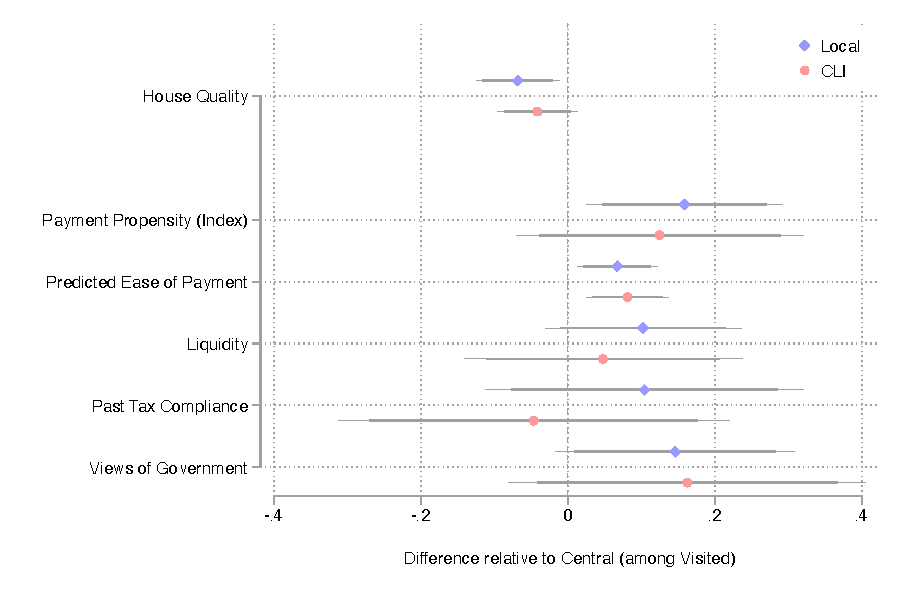
\includegraphics[scale=.62]{Output/chars_visited.pdf}\\
B: Predicted Ease of Payment and House Quality\\
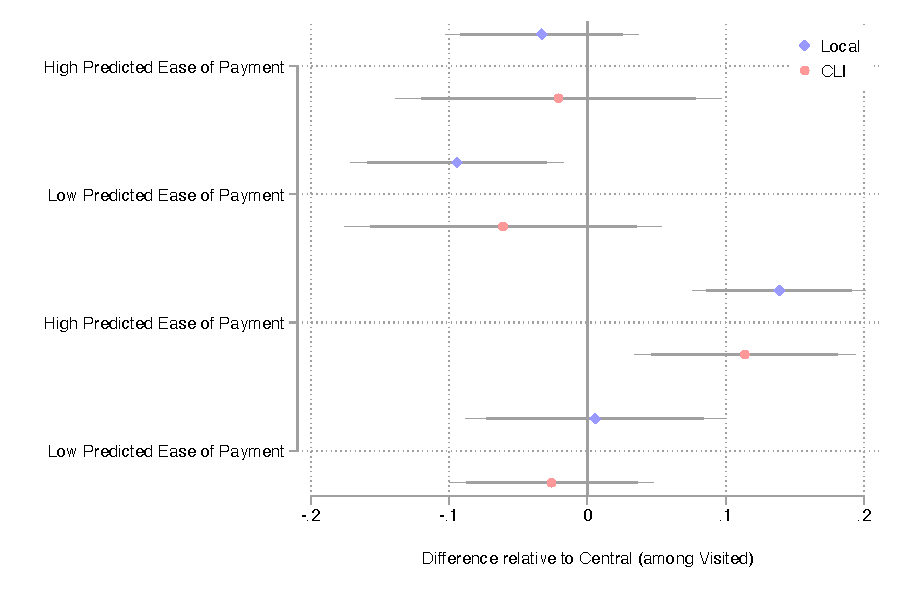
\includegraphics[scale=.8]{Output/chars_PEXHQ.pdf}\\
\end{tabular}
\usebox{\tablebox}\\[1ex]
\parbox{6in}{\footnotesize \textit{Notes}: This figure reports differences by treatment arm in the characteristics of properties visited by collectors after registration, showing differences in characteristics of visited properties in the Local and CLI arms relative to the Central arm.  Panel A shows differences in visible and non-visible characteristics for indices described in Section \ref{targeting_discussion}.  Panel B shows differences in the probability of receiving a visit in the four cells indicated (defined by interactions of high/low dummies for household house quality and predicted ease of payment). Differences are estimated through separate regressions of characteristics on a treatment indicator among visited properties, controlling for the leave-one-out neighborhood mean of the outcome (Panel A) or the neighborhood mean of house quality and ease of payment (Panel B). We include time period, house type, and stratum fixed effects. We cluster standard errors at the neighborhood level. Households that paid during registration are dropped. As a comparison, Figure \ref{main_targeting_appendix} shows the correlations between tax visits and household characteristics within treatments, rather than differences across treatments. Figures \ref{fig:main_targeting1_NoHouseFE} and \ref{main_targeting_noControlMean_appendix} replicate this analysis while omitting house fixed effects and neighborhood mean controls, respectively. We discuss these results in Section \ref{targeting_discussion}.}
\end{figure}


\begin{figure}[H]
	\centering{}\caption*{
		\label{fig:main_targeting1_R1} Figure \ref{fig:main_targeting1} Replicated using Oprobit}
	\centering
	\centerfloat
	\begin{tabular}{c}
		A: Visible and Non-Visible Characteristics\\
		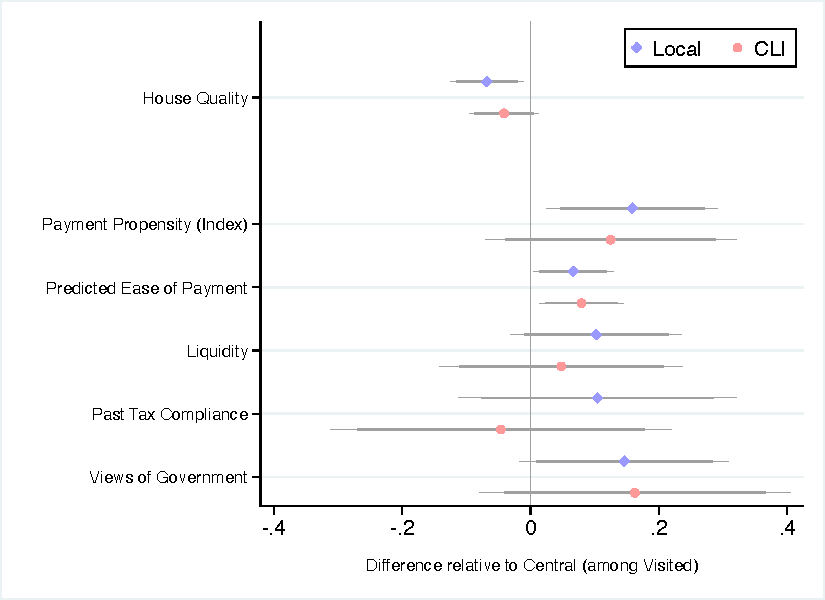
\includegraphics[scale=.62]{Output/chars_visitedR1.pdf}\\
		B: Predicted Ease of Payment and House Quality\\
		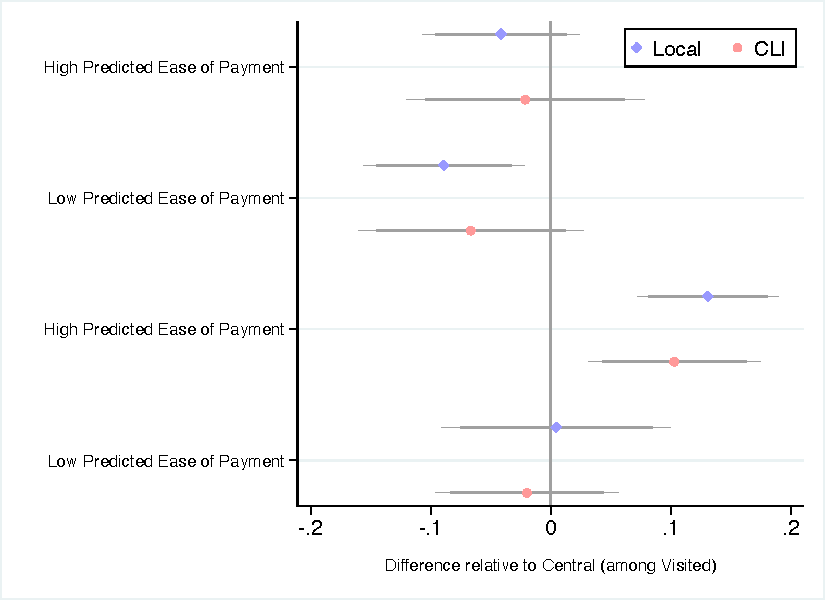
\includegraphics[scale=.8]{Output/chars_PEXHQ_R1.pdf}\\
	\end{tabular}
	\usebox{\tablebox}\\[1ex]
	\parbox{6in}{\footnotesize \textit{Notes}:  \ref{targeting_discussion}.}
\end{figure}

\begin{figure}[H]
	\centering{}\caption*{
		\label{fig:main_targeting1_R2} Figure \ref{fig:main_targeting1} Replicated using Oprobit and Controlling for Chiefs Characteristics}
	\centering
	\centerfloat
	\begin{tabular}{c}
		A: Visible and Non-Visible Characteristics\\
		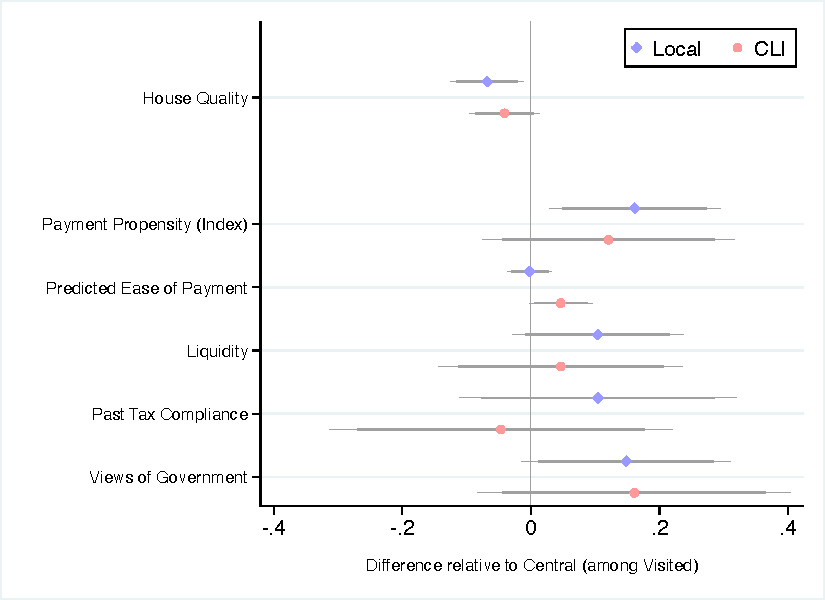
\includegraphics[scale=.62]{Output/chars_visited_R2.pdf}\\
		B: Predicted Ease of Payment and House Quality\\
		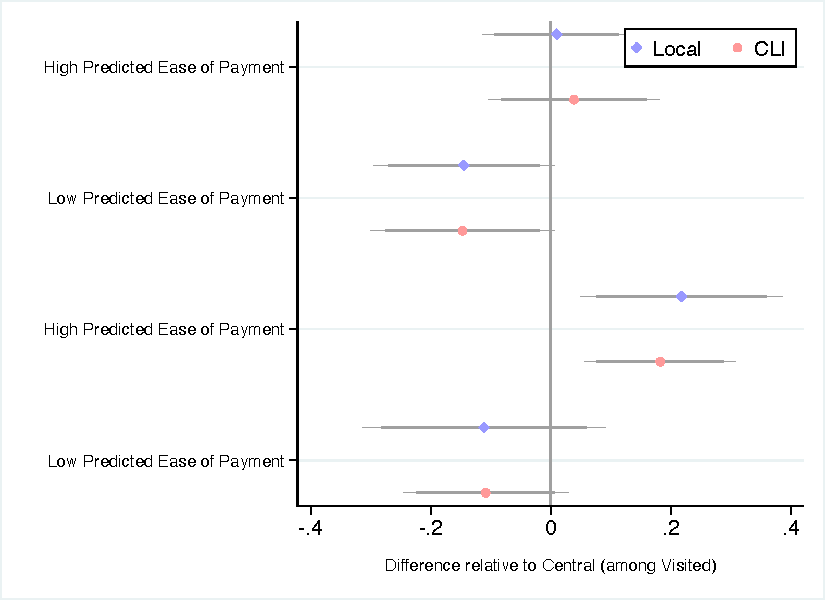
\includegraphics[scale=.8]{Output/chars_PEXHQ_R2.pdf}\\
	\end{tabular}
	\usebox{\tablebox}\\[1ex]
	\parbox{6in}{\footnotesize \textit{Notes}:  \ref{targeting_discussion}.}
\end{figure}

%%%%%%%%%%%%%%%%%%%%%%%%%%%%%%%%%%%%%%%%%%%%%%%%%%%%%%%%%%%%%%%%%

\begin{table}[H]
\textbf{\caption{\label{Table_CvL_Distribution_Incidence} Local v. Central: The Distribution of the Tax Burden}}
\centering
\begin{lrbox}{\tablebox}
\resizebox{15cm}{!}{
{
\def\sym#1{\ifmmode^{#1}\else\(^{#1}\)\fi}
\begin{tabular}{l*{5}{c}}
\hline\hline
                &\multicolumn{1}{c}{Paid - Periph}&\multicolumn{1}{c}{Paid - MM}&\multicolumn{1}{c}{HQ - Visited}&\multicolumn{1}{c}{HQ - Paid}&\multicolumn{1}{c}{Income - Visited}\\
                &\multicolumn{1}{c}{(1)}         &\multicolumn{1}{c}{(2)}         &\multicolumn{1}{c}{(3)}         &\multicolumn{1}{c}{(4)}         &\multicolumn{1}{c}{(5)}         \\
\hline
Local           &    0.036\sym{***}&    0.002         &   -0.146\sym{**} &    0.002         &   -0.063         \\
                &  (0.008)         &  (0.013)         &  (0.057)         &  (0.042)         &  (0.167)         \\
a7\_hq\_y         &                  &                  &    0.940\sym{***}&                  &                  \\
                &                  &                  &  (0.041)         &                  &                  \\
a7\_inc\_mo\_avg   &                  &                  &                  &    0.001         &                  \\
                &                  &                  &                  &  (0.020)         &                  \\
a7\_econ\_ind     &                  &                  &                  &                  &    0.289         \\
                &                  &                  &                  &                  &  (0.270)         \\
Month FE        &      Yes         &      Yes         &      Yes         &      Yes         &      Yes         \\
House FE        &       No         &       No         &      Yes         &      Yes         &      Yes         \\
Stratum FE      &      Yes         &      Yes         &      Yes         &      Yes         &      Yes         \\
\hline
Observations    &    24380         &     3384         &     1310         &      228         &      228         \\
Clusters        &      208         &      150         &      157         &      121         &      121         \\
Mean            &     .064         &     .062         &     .099         &     .007         &     .118         \\
\hline\hline
\end{tabular}
}

}
\end{lrbox}
\usebox{\tablebox}\\[1ex]
\parbox{6in}{\footnotesize \textit{Notes}: This table reports estimates from a version of Equation \ref{equation_cvl}, comparing property tax compliance in Local and Central (the excluded category). We include fixed effects for house type, randomization strata, and time periods, as described in Section \ref{estimation}, and we cluster standard errors at the neighborhood level. Columns 1 and 2 report estimates of the impact of local collection on compliance for low- and high-band households, respectively. Column 3 reports differences in an index of house quality conditional on the property paying the tax.  Column 4 reports differences in monthly household income of properties, averaged across baseline and endline values, in Congolese Francs, conditional on paying the tax.  Column 5 reports differences in an index of liquidity measures drawn from baseline (excepting income, which is also included, and uses information from endline) among payers. Columns 3--5 control for the leave-one-out neighborhood mean of the outcome. For robustness, we re-estimate these results excluding (\textit{i}) property type fixed effects (Table \ref{Table_CvL_Distribution_Incidence_NoHouseFE}) and (\textit{ii}) leave-one-out neighborhood mean controls (Table \ref{Table_CvLvCLI_Distribution_Incidence}). We also estimate (\textit{iii}) an interacted version of the house type regressions in Columns 1--2 (Table \ref{PaperTable_CvL_Incidence_HouseTypeInteraction}) and (\textit{iv}) an alternative version of Columns 3--5 in tax compliance is regressed on indicators for having complier characteristics above the median value in the sample are interacted, a Local treatment indicator, and the interaction (Table \ref{PaperTable_CvL_Incidence_Cols3to5Interactions}). Figure \ref{fig:distribution_all} (Panel B) shows the distribution of house quality among tax compliers across treatments. We discuss the interpretation of these results in Section \ref{incidence_discussion}.}
\end{table}



\begin{table}[H]
	\textbf{\caption*{\label{Table_CvL_Distribution_Incidence_Replicated} Table \ref{Table_CvL_Distribution_Incidence}  $\rightarrow$  Replicated using RI}}
	\centering
	\begin{lrbox}{\tablebox}
		\resizebox{15cm}{!}{
			{
\def\sym#1{\ifmmode^{#1}\else\(^{#1}\)\fi}
\begin{tabular}{l*{5}{c}}
\toprule
                &\multicolumn{1}{c}{Paid - Periph}&\multicolumn{1}{c}{Paid - MM}&\multicolumn{1}{c}{HQ - Visited}&\multicolumn{1}{c}{HQ - Paid}&\multicolumn{1}{c}{Income - Visited}\\
                &\multicolumn{1}{c}{(1)}&\multicolumn{1}{c}{(2)}&\multicolumn{1}{c}{(3)}&\multicolumn{1}{c}{(4)}&\multicolumn{1}{c}{(5)}\\
                &b/p/pvalues&b/p/pvalues&b/p/pvalues&b/p/pvalues&b/p/pvalues\\
\midrule
Local           &0.0362650&0.00164441&-0.146327&0.00192675&-0.0629973\\
                &(0.0000106)&  (0.898)& (0.0106)&  (0.963)&  (0.707)\\
                &[0.001000]&[0.903000]&[0.018000]&[0.962000]&[0.695000]\\
a7\_hq\_y         &         &         & 0.940466&         &         \\
                &         &         &(3.22e-52)&         &         \\
                &         &         &         &         &         \\
a7\_inc\_mo\_avg   &         &         &         &0.000598220&         \\
                &         &         &         &  (0.977)&         \\
                &         &         &         &         &         \\
a7\_econ\_ind     &         &         &         &         & 0.288814\\
                &         &         &         &         &  (0.286)\\
                &         &         &         &         &         \\
Month FE        &      Yes&      Yes&      Yes&      Yes&      Yes\\
House FE        &       No&       No&      Yes&      Yes&      Yes\\
Stratum FE      &      Yes&      Yes&      Yes&      Yes&      Yes\\
\midrule
Observations    &    24380&     3384&     1310&      228&      228\\
Clusters        &      208&      150&      157&      121&      121\\
Mean            &     .064&     .062&     .099&     .007&     .118\\
\bottomrule
\end{tabular}
}

		}
	\end{lrbox}
	\usebox{\tablebox}\\[1ex]
	\parbox{6in}{\footnotesize \textit{Notes}: }
\end{table}


%%%%%%%%%%%%%%%%%%%%%%%%%%%%%%%%%%%%%%%%%%%%%%%%%%%%%%%%%%%%%%%%%

\FloatBarrier
\singlespace

%%%%%%%%%%%%%%%%%%%%%%%%%%%%%%%%%%%%%%%%%%%

\clearpage

%%%%%%%%%%%%%%%%%%%%%%%%%%%%%%%%%%%%%%%%%%%

\appendix
\vspace{-1cm}
\section*{\centering \Huge{Supplementary Data and Appendix} \\ \LARGE{For Online Publication}}

%%%%%%%%%%%%%%%%%%%%%%%%%%%%%%%%%%%%%%%%%%%

\startcontents

%%%%%%%%%%%%%%%%%%%%%%%%%%%%%%%%%%%%%%%%%%%%%%%%%%%%%%%%%%%%%%%%%

\setcounter{table}{0}
\renewcommand{\thetable}{A\arabic{table}}
\setcounter{figure}{0}
\renewcommand{\thefigure}{A\arabic{figure}}
\setcounter{section}{0}
\renewcommand{\thesection}{A\arabic{section}}

%%%%%%%%%%%%%%%%%%%%%%%%%%%%%%%%%%%%%%%%%%%%%%%%%%%%%%%%%%%%%%%%%

\section{Additional Exhibits for the Main Analysis}

%%%%%%%%%%%%%%%%%%%%%%%%%%%%%%%%%%%%%%%%%%%%%%%%%%%%%%%%%%%%%%%%%

\FloatBarrier

%%%%%%%%%%%%%%%%%%%%%%%%%%%%%%%%%%%%%%%%%%%%%%%%%%%%%%%%%%%%%%%%%

\subsection{Additional Exhibits for Paper Section 2 --- Setting}

%%%%%%%%%%%%%%%%%%%%%%%%%%%%%%%%%%%%%%%%%%%%%%%%%%%%%%%%%%%%%%%%%

\begin{figure}[H]
\centering{}\caption{Sample tax notice \label{fig:flyerPG_L}}
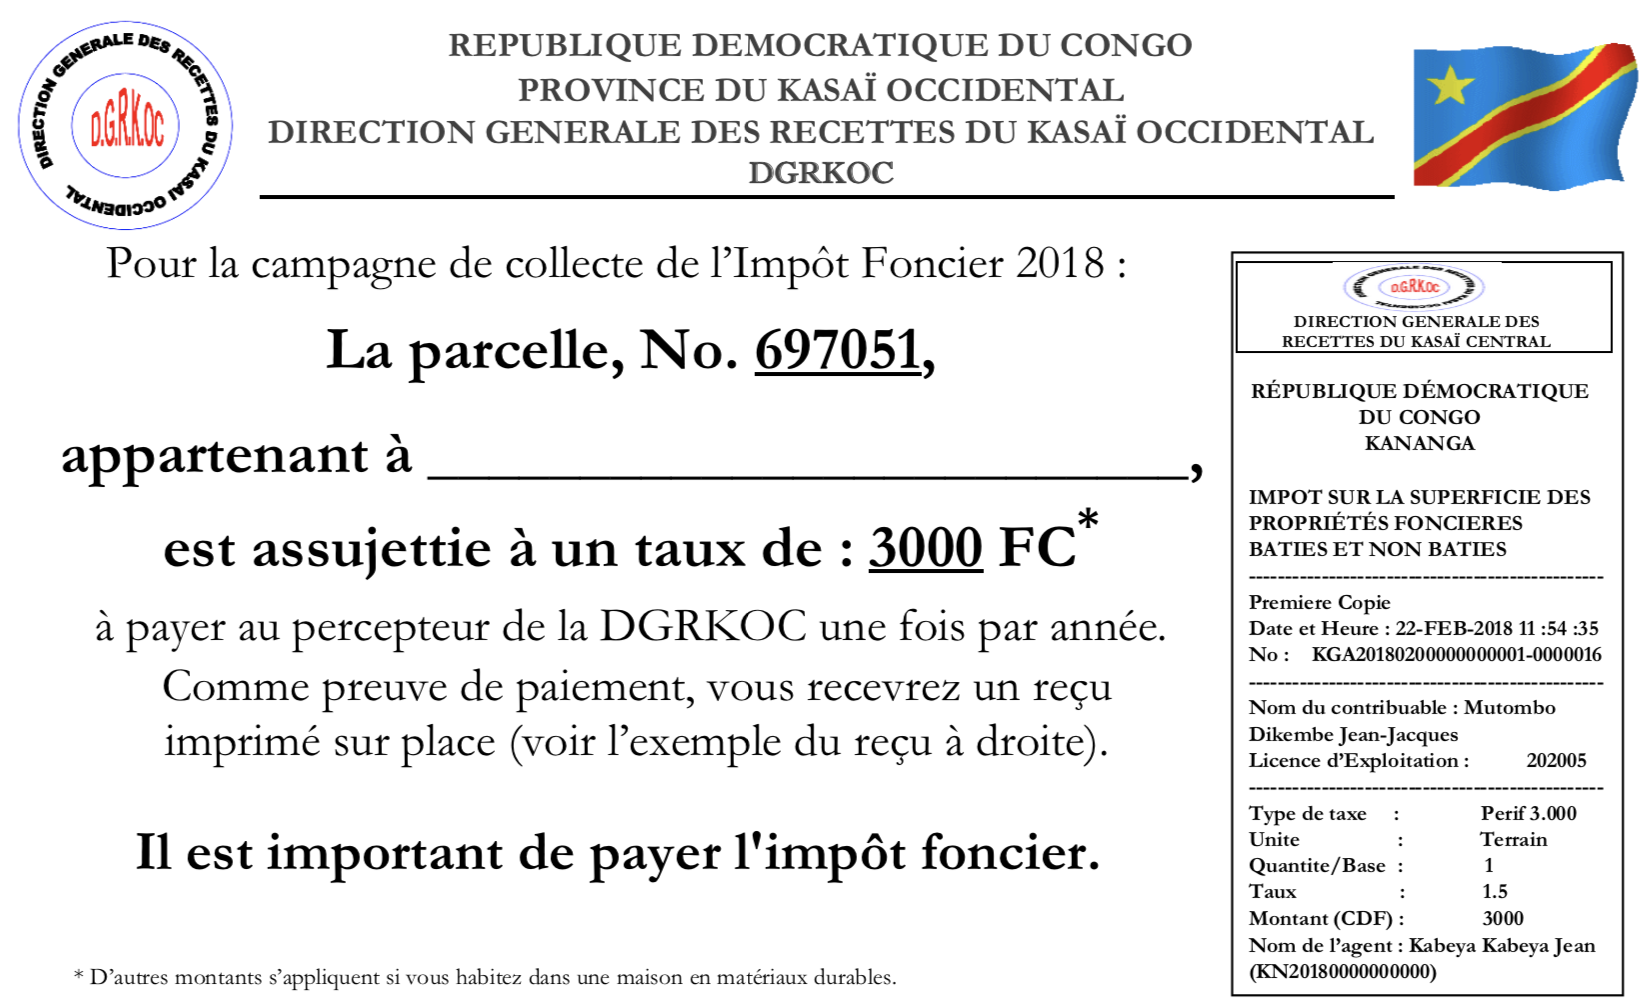
\includegraphics[scale=0.5]{Documents/flier3000control.png} 
\usebox{\tablebox}\\[1ex]
\parbox{6in}{\footnotesize \textit{Notes}: This figure displays a sample tax notice, which is discussed in Section \ref{mechanics}. The flier says: ``For the 2018 property tax collection campaign: the compound 697051 belonging to [name of owner] is subject to a tax rate of 3000 CF to be paid to a DGRKOC collector once per year. As proof of payment, you will receive a receipt printed on the spot (see example to the right). It is important to pay the property tax.'' The footnote says ``Other amounts apply if you live in a house built of durable materials.'' This flier contains the Control message (``It is important to pay the property tax''), discussed in the text in Section \ref{persuasion} and in detail in Section \ref{information_treatments}. A version of the flier in Tshiluba, the primary local language, was printed on the opposite side. Fliers were identical across treatment arms.}
\end{figure}

%%%%%%%%%%%%%%%%%%%%%%%%%%%%%%%%%%%%%%%%%%%%%%%%%%%%%%%%%%%%%%%%%

\subsection{Additional Exhibits for Paper Section 3 --- Design}

%%%%%%%%%%%%%%%%%%%%%%%%%%%%%%%%%%%%%%%%%%%%%%%%%%%%%%%%%%%%%%%%%

\begin{figure}[H]
\centering{}\caption{The unit of randomization: neighborhoods of Kananga \label{fig:polygons}}
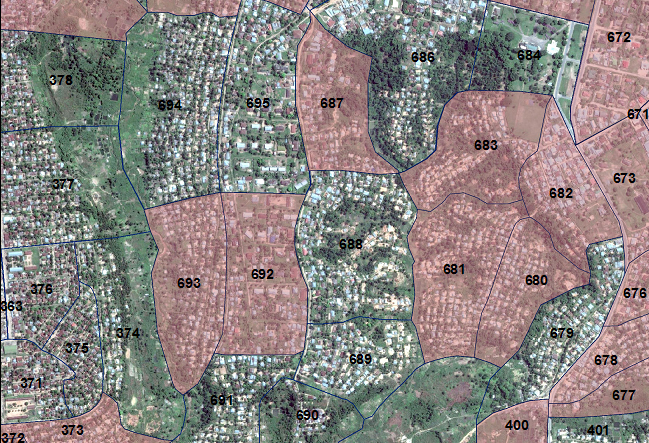
\includegraphics[scale=0.9]{Documents/polygons.png}
\usebox{\tablebox}\\[1ex]
\parbox{6in}{\footnotesize \textit{Notes}: This figure displays a sample of neighborhood divisions in Kananga, which are discussed in Section \ref{randomization}.}
\end{figure}

%%%%%%%%%%%%%%%%%%%%%%%%%%%%%%%%%%%%%%%%%%%%%%%%%%%%%%%%%%%%%%%%%

\begin{figure}[H]
\centering{}\caption{Geographic strata \label{fig:strata}}
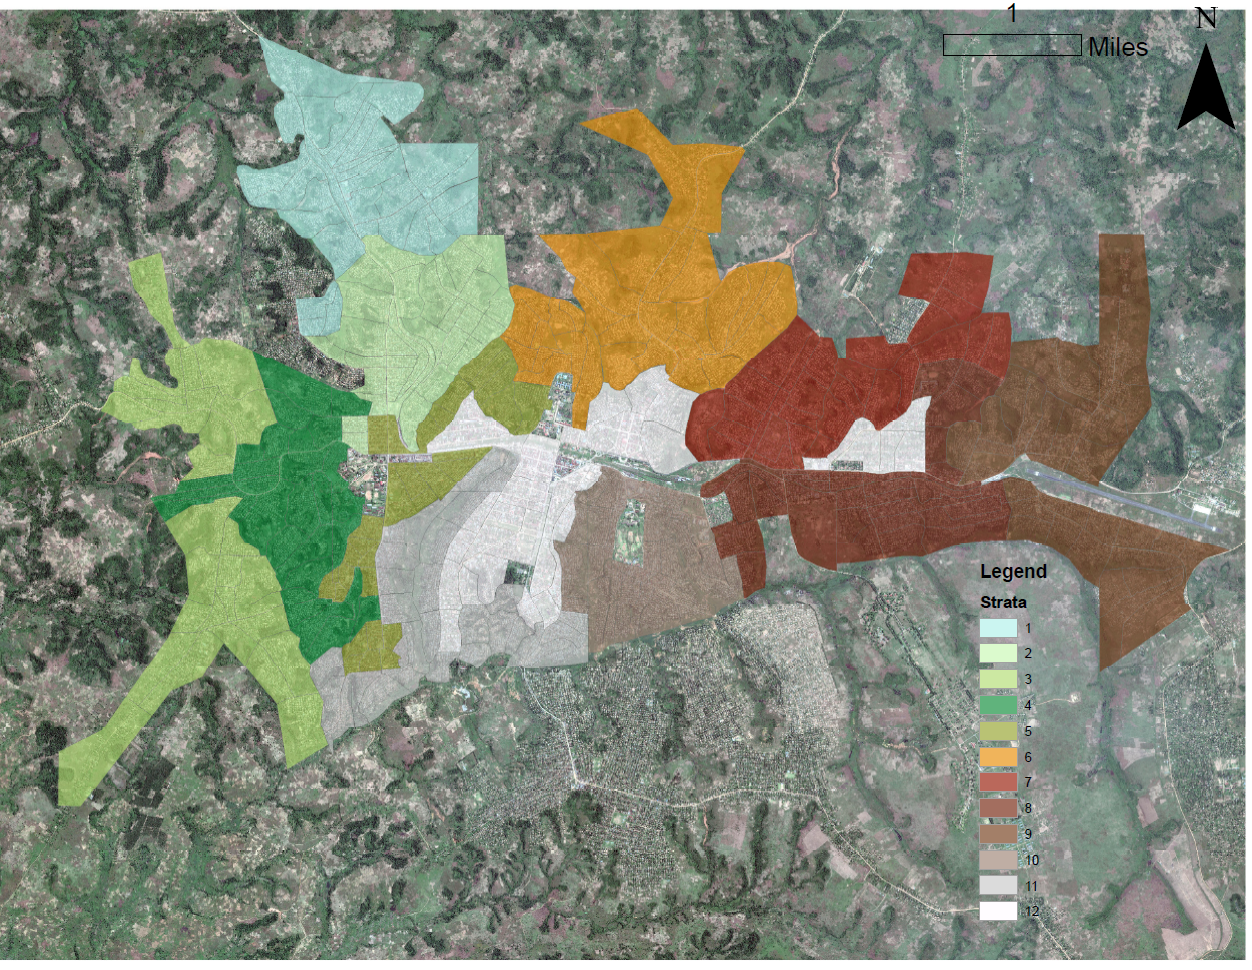
\includegraphics[scale=0.7]{Documents/strata.png}
\caption*{\footnotesize{\upshape{\textnormal{\textit{Notes}: This figure displays the geographic strata of Kananga, which are discussed in Section \ref{randomization}.}}}}
\end{figure}

%%%%%%%%%%%%%%%%%%%%%%%%%%%%%%%%%%%%%%%%%%%%%%%%%%%%%%%%%%%%%%%%%

\begin{table}[H]
\textbf{\caption{\label{comparing_collectors} Local v. Central: Collector Characteristics}}
\centering
\begin{lrbox}{\tablebox}
\scalebox{0.935}{
\begin{tabular}{l*{3}c}
\hline\hline
 & (1) & (2) & (3) \\
Variable & Central collectors & Local Collectors & Difference \\
\hline
Age&30.760&58.712&27.952***\\
&(8.098)&(11.031)&(1.740)\\
\% Female&0.060&0.045&-0.015\\
&(0.240)&(0.208)&(0.037)\\
Born in Kananga&0.480&0.607&0.127\\
&(0.505)&(0.491)&(0.085)\\
Log Monthly Income&4.238&4.045&-0.192\\
&(0.969)&(1.153)&(0.189)\\
Number of Possessions&1.820&1.044&-0.776***\\
&(1.320)&(1.263)&(0.218)\\
Education years&16.940&13.266&-3.674***\\
&(3.413)&(3.487)&(0.592)\\
Works Other Job&0.682&0.761&0.079\\
&(0.471)&(0.428)&(0.078)\\
Test Maths (Mean)&0.745&0.743&-0.002\\
&(0.234)&(0.258)&(0.043)\\
Reading Ability (Mean)&1.770&1.838&0.068\\
&(0.612)&(0.779)&(0.124)\\
Trust in Gov. (Mean)&3.033&2.716&-0.317*\\
&(0.732)&(1.051)&(0.165)\\
Prov. Gov. Capacity (Mean)&150.178&158.660&8.482\\
&(73.893)&(99.387)&(15.690)\\
Poor Priority (Mean)&2.680&2.758&0.078\\
&(0.563)&(0.588)&(0.099)\\
Progressiveness (Mean)&2.584&2.470&-0.114**\\
&(0.285)&(0.308)&(0.051)\\
\hline
Observations & 50 & 113 & 163 \\
\hline\hline
\end{tabular}

}
\end{lrbox}
\usebox{\tablebox}\\[1ex]
\parbox{6in}{\footnotesize \textit{Notes}: This table compares baseline characteristics of state collectors in  neighborhoods assigned to the Central treatment arm (Column 1) and chiefs in neighborhoods assigned to the Local treatment arm (Column 2). Column 3 reports a simple difference-in-means test. The data come from surveys conducted with tax collectors before the 2018 campaign. The first seven variables are the respondent's age, a sex indicator, an indicator for being born in Kananga, log monthly income, wealth (defined as the number of possessions: motorbike, car, radio, TV, generator and sewing machine), years of education, and an indicator for working another job during the tax campaign. \textit{Math Ability} and \textit{Reading Ability} are collectors' average score on a series of quiz-type questions. The last four measures concern attitudes about the government and redistribution, measured through survey questions with Likert-scale response options. These comparisons are discussed in Section \ref{treatment_arms}.}
\end{table}

%%%%%%%%%%%%%%%%%%%%%%%%%%%%%%%%%%%%%%%%%%%%%%%%%%%%%%%%%%%%%%%%%

\begin{figure}[H]
\textbf{\caption{Collector Performance and Education / Wealth \label{collector_chars_ability}}}
\centering
\begin{tabular}{cc}
\\
A: State collectors' Education Level & B: Chief collectors'  Education Level   \\
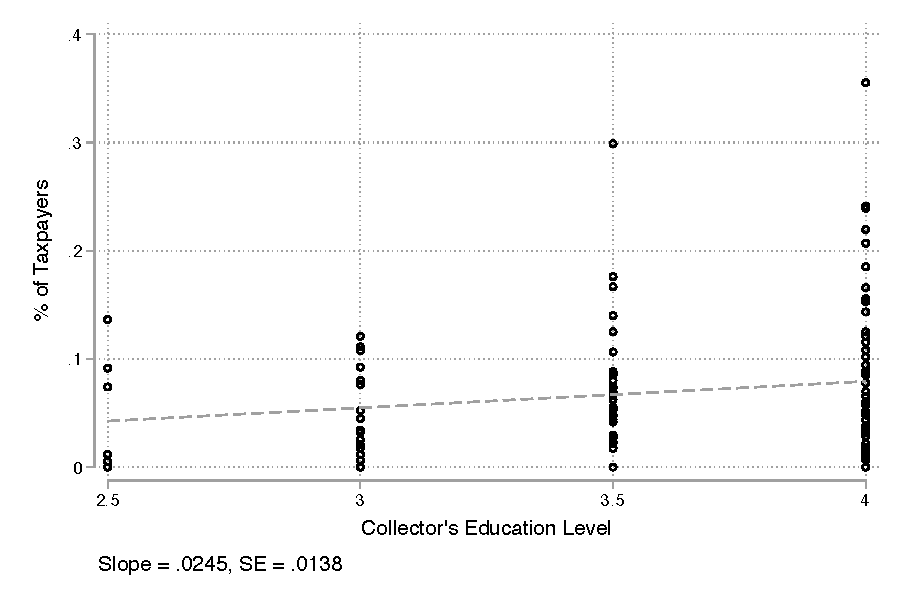
\includegraphics[scale=0.5]{Output/taxes_paid_DGRKOC_educ_lvl.pdf} & 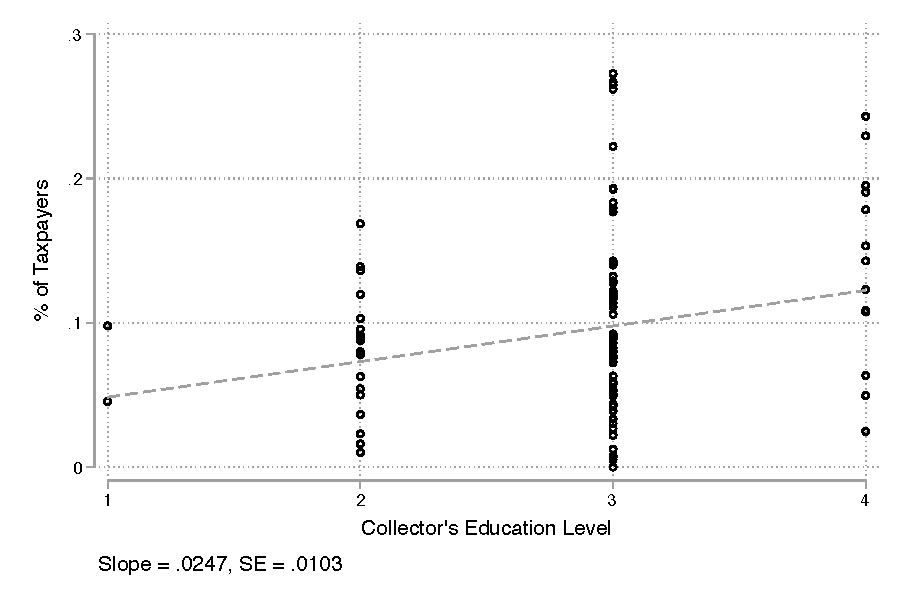
\includegraphics[scale=0.5]{Output/taxes_paid_chief_educ_lvl.pdf}\\
C: State collectors' Years of Education    & D:  Chief collectors'  Years of Education   \\
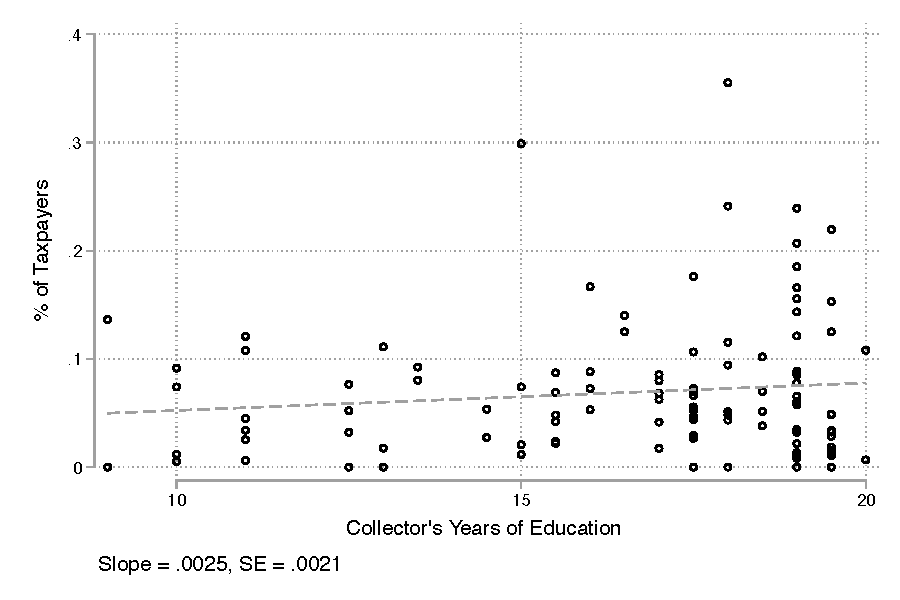
\includegraphics[scale=0.5]{Output/taxes_paid_DGRKOC_educ_yrs.pdf} & 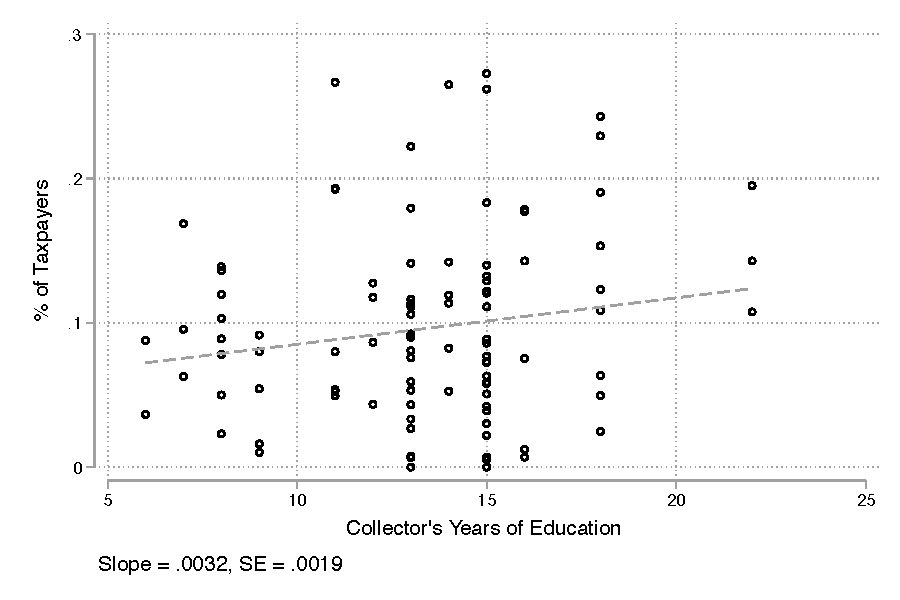
\includegraphics[scale=0.5]{Output/taxes_paid_chief_educ_yrs.pdf}\\
E: State collectors' \# Assets / possessions & F:  Chief collectors' \# Assets / possessions    \\
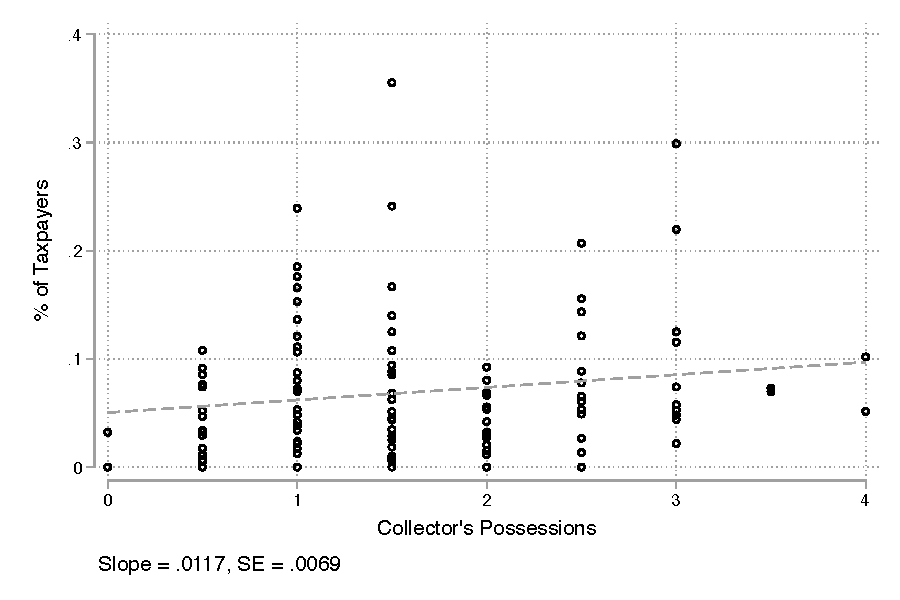
\includegraphics[scale=0.5]{Output/taxes_paid_DGRKOC_possessions_nb.pdf} & 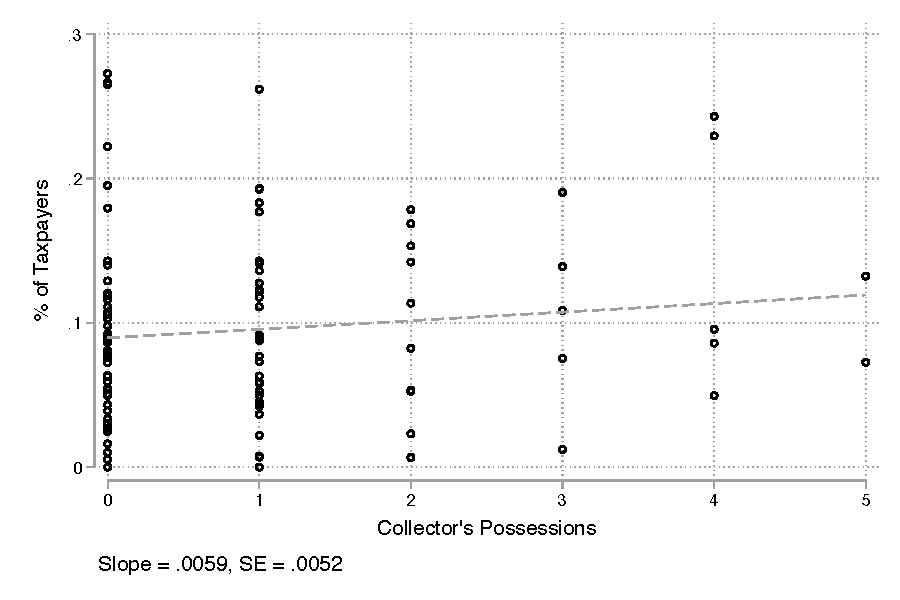
\includegraphics[scale=0.5]{Output/taxes_paid_chief_possessions_nb.pdf}\\
\end{tabular}
\caption*{\footnotesize{\upshape{\textnormal{\textit{Notes}: This figure shows the relationship between tax compliance in the neighborhood and tax collectors' education levels (Panels A and B), years of education (Panels C and D), and wealth (Panels E and F). Wealth here is defined as number of possessions among the following: motorbike, car, radio, TV, generator, and sewing machine. The relationships are reported separately for neighborhoods assigned to the Central and CLI treatment arms where tax collection was done by state agents (Panels A, C, and E) and for neighborhoods assigned to the Local treatment arm where tax collection was done by city chiefs (Panel B, D, and F). These comparisons are discussed in Section \ref{treatment_arms}}}}}
\end{figure}

%%%%%%%%%%%%%%%%%%%%%%%%%%%%%%%%%%%%%%%%%%%%%%%%%%%%%%%%%%%%%%%%%

\begin{table}[H]
\textbf{\caption{Randomization Balance: Bilateral Treatment Comparisons}\label{tab:balance_tests_F}}
\centering
\tiny{{
\def\sym#1{\ifmmode^{#1}\else\(^{#1}\)\fi}
\begin{tabular}{l*{3}{c}}
\hline\hline
                &\multicolumn{1}{c}{Percentage Paid in 2016}&\multicolumn{2}{c}{Affected by Conflict in 2016}\\
                &\multicolumn{1}{c}{(1)}         &\multicolumn{1}{c}{(2)}         &\multicolumn{1}{c}{(3)}         \\
\hline
rev\_2016\_alternate&    0.000         &   -0.000         &   -0.000         \\
                &  (0.000)         &  (0.000)         &  (0.000)         \\
rouge           &    0.132         &   -0.131         &    0.444\sym{**} \\
                &  (0.289)         &  (0.362)         &  (0.215)         \\
Stratum FE      &      Yes         &      Yes         &      Yes         \\
\hline
Observations    &      221         &      190         &      160         \\
Clusters        &      221         &      190         &      160         \\
Mean            &                  &                  &                  \\
F\_stat          &                  &                  &                  \\
p\_val           &                  &                  &                  \\
\hline\hline
\end{tabular}
}
}
\tiny{{
\def\sym#1{\ifmmode^{#1}\else\(^{#1}\)\fi}
\begin{tabular}{l*{3}{c}}
\hline\hline
                &\multicolumn{1}{c}{Years of Education}&\multicolumn{1}{c}{Electricity}&\multicolumn{1}{c}{Log HH Monthly Income}\\
                &\multicolumn{1}{c}{(1)}         &\multicolumn{1}{c}{(2)}         &\multicolumn{1}{c}{(3)}         \\
\hline
edu\_yrs         &   -0.003         &    0.001         &   -0.003         \\
                &  (0.003)         &  (0.003)         &  (0.003)         \\
Do you have any source of electricity at your home?&    0.008         &    0.021         &    0.030         \\
                &  (0.027)         &  (0.031)         &  (0.031)         \\
lg\_inc\_mo       &    0.006         &   -0.003         &   -0.006         \\
                &  (0.005)         &  (0.005)         &  (0.005)         \\
Local leaders   &    0.012         &    0.026\sym{**} &    0.026\sym{**} \\
                &  (0.012)         &  (0.012)         &  (0.013)         \\
The national government (in Kinshasa)&   -0.015         &   -0.010         &   -0.002         \\
                &  (0.014)         &  (0.012)         &  (0.013)         \\
The provincial government&    0.026         &    0.018         &   -0.001         \\
                &  (0.016)         &  (0.015)         &  (0.016)         \\
The tax ministry&   -0.001         &   -0.008         &   -0.003         \\
                &  (0.010)         &  (0.012)         &  (0.012)         \\
Stratum FE      &      Yes         &      Yes         &      Yes         \\
\hline
Observations    &     2117         &     1768         &     1501         \\
Clusters        &      221         &      187         &      159         \\
Mean            &                  &                  &                  \\
F\_stat          &                  &                  &                  \\
p\_val           &                  &                  &                  \\
\hline\hline
\end{tabular}
}
}
\tiny{{
\def\sym#1{\ifmmode^{#1}\else\(^{#1}\)\fi}
\begin{tabular}{l*{3}{c}}
\hline\hline
                &\multicolumn{1}{c}{Years of Education}&\multicolumn{1}{c}{Electricity}&\multicolumn{1}{c}{Log HH Monthly Income}\\
                &\multicolumn{1}{c}{(1)}         &\multicolumn{1}{c}{(2)}         &\multicolumn{1}{c}{(3)}         \\
\hline
edu\_yrs         &   -0.003         &    0.001         &   -0.003         \\
                &  (0.003)         &  (0.003)         &  (0.003)         \\
Do you have any source of electricity at your home?&    0.008         &    0.021         &    0.030         \\
                &  (0.027)         &  (0.031)         &  (0.031)         \\
lg\_inc\_mo       &    0.006         &   -0.003         &   -0.006         \\
                &  (0.005)         &  (0.005)         &  (0.005)         \\
Local leaders   &    0.012         &    0.026\sym{**} &    0.026\sym{**} \\
                &  (0.012)         &  (0.012)         &  (0.013)         \\
The national government (in Kinshasa)&   -0.015         &   -0.010         &   -0.002         \\
                &  (0.014)         &  (0.012)         &  (0.013)         \\
The provincial government&    0.026         &    0.018         &   -0.001         \\
                &  (0.016)         &  (0.015)         &  (0.016)         \\
The tax ministry&   -0.001         &   -0.008         &   -0.003         \\
                &  (0.010)         &  (0.012)         &  (0.012)         \\
Stratum FE      &      Yes         &      Yes         &      Yes         \\
\hline
Observations    &     2117         &     1768         &     1501         \\
Clusters        &      221         &      187         &      159         \\
Mean            &                  &                  &                  \\
F\_stat          &                  &                  &                  \\
p\_val           &                  &                  &                  \\
\hline\hline
\end{tabular}
}
}
\usebox{\tablebox}\\[1ex]
\parbox{6in}{\footnotesize 
\textit{Notes:} This table summarizes balance tests for bilateral treatment comparisons. Each column compares the noted treatment arm to Central. The bottom row of each panel contains the statistics for tests of the omnibus null hypothesis that the treatment effects for the covariates studied in Table \ref{tab:balance_tests} are all zero using parametric $F$ tests. As usual, regressions include stratum fixed effects and cluster standard errors at the neighborhood level.  We run separate tests for variables drawn from baseline survey, midline survey, and neighborhood-level data to maximize the number of observations included in each regression. Midline characteristics include the distance characteristics from registration reported in Table \ref{tab:balance_tests}. We discuss these results in Section \ref{balance}.}
\end{table}

%%%%%%%%%%%%%%%%%%%%%%%%%%%%%%%%%%%%%%%%%%%%%%%%%%%%%%%%%%%%%%%%%

\begin{table}[H]
\textbf{\caption{Randomization Balance: Including Control Group}\label{tab:balance_tests_wcontrol}}
\centering
\tiny{\csvautotabular[respect underscore=true]{Output/balance_baseline_wcontrol.csv}}
\\
\tiny{\csvautotabular[respect underscore=true]{Output/balance_midline_wcontrol.csv}}
\small{{
\def\sym#1{\ifmmode^{#1}\else\(^{#1}\)\fi}
\begin{tabular}{l*{3}{c}}
\hline\hline
                &\multicolumn{1}{c}{Baseline to Endline Attrition}&\multicolumn{1}{c}{Baseline Replacement}&\multicolumn{1}{c}{Midline Attrition}\\
                &\multicolumn{1}{c}{(1)}         &\multicolumn{1}{c}{(2)}         &\multicolumn{1}{c}{(3)}         \\
\hline
central         &   -0.024         &   -0.015         &   -0.047         \\
                &  (0.051)         &  (0.041)         &  (0.056)         \\
local           &   -0.040         &   -0.004         &   -0.026         \\
                &  (0.051)         &  (0.040)         &  (0.058)         \\
centralwinfo    &   -0.045         &   -0.007         &   -0.058         \\
                &  (0.051)         &  (0.041)         &  (0.056)         \\
centralxlocal   &   -0.064         &    0.002         &   -0.103\sym{*}  \\
                &  (0.051)         &  (0.046)         &  (0.058)         \\
\hline
Observations    &     4246         &     3483         &    45162         \\
Clusters        &      356         &      356         &      356         \\
Mean            &     .133         &     .174         &     .256         \\
\hline\hline
\end{tabular}
}
}
\usebox{\tablebox}\\[1ex]
\parbox{6in}{\footnotesize 
\textit{Notes:} This table reports the coefficients from balance tests estimated by regressing characteristics for property owners (Panel A), properties (Panel B), and neighborhoods (Panel C) on treatment indicators, clustering standard errors at the neighborhood level. Panel D shows differences in attrition from baseline to endline surveying, replacement at endline of baseline respondents, and attrition from registration to midline surveying. The Control arm is the excluded category. Randomization stratum fixed effects are not included because Control neighborhoods do not exist in every strata. Superscripts $B$, $M$, and $R$ denote which variables come from baseline, midline, and registration, respectively. Variables are described in Section \ref{variable_descriptions}. Joint orthogonality tests for specific treatment comparisons are shown in Table \ref{tab:balance_tests_F}. We discuss these results in Section \ref{balance}.}
\end{table}

%%%%%%%%%%%%%%%%%%%%%%%%%%%%%%%%%%%%%%%%%%%%%%%%%%%%%%%%%%%%%%%%%

\begin{table}[H]
\vspace{.5cm}
\textbf{\caption{Midline Non-Response Across Treatments}
\label{midline_nonresp_F}}
\centering
\begin{lrbox}{\tablebox}
\scalebox{0.9}{
{
\def\sym#1{\ifmmode^{#1}\else\(^{#1}\)\fi}
\begin{tabular}{l*{3}{c}}
\hline\hline
                &\multicolumn{1}{c}{(1)}         &\multicolumn{1}{c}{(2)}         &\multicolumn{1}{c}{(3)}         \\
\hline
Sex Missing     &    0.181         &   -0.081\sym{**} &    0.388\sym{*}  \\
                &  (0.317)         &  (0.035)         &  (0.214)         \\
Age Missing     &   -0.304         &   -0.090\sym{**} &   -0.460\sym{**} \\
                &  (0.319)         &  (0.038)         &  (0.214)         \\
Majority Tribe Missing&    0.026         &    0.035         &    0.025         \\
                &  (0.024)         &  (0.025)         &  (0.023)         \\
Employed Missing&   -0.348         &    0.097\sym{*}  &    0.044         \\
                &  (0.220)         &  (0.057)         &  (0.040)         \\
Salaried Missing&    0.368\sym{*}  &   -0.060         &   -0.031         \\
                &  (0.217)         &  (0.051)         &  (0.032)         \\
Relative Works for Government Missing&   -0.002         &    0.002         &    0.002         \\
                &  (0.032)         &  (0.033)         &  (0.030)         \\
Stratum FE      &      Yes         &      Yes         &      Yes         \\
\hline
Observations    &    22533         &    18927         &    16494         \\
Clusters        &      221         &      189         &      160         \\
F\_stat          &                  &                  &                  \\
p\_val           &                  &                  &                  \\
\hline\hline
\end{tabular}
}

}
\end{lrbox}
\usebox{\tablebox}\\[1ex]
\parbox{6in}{\footnotesize 
\textit{Notes:} This table summarizes tests for differential midline non-response. Each column compares the noted treatment arm to Central. The bottom row of each panel contains the statistics for tests of the omnibus null hypothesis that the treatment effects for all the variables listed are zero using parametric $F$-tests. As usual, regressions include stratum fixed effects and cluster standard errors at the neighborhood level. The \textit{Works for Government} variable is omitted as it is defined from the same underlying variable as \textit{Salaried} and is thus collinear.}
\end{table}

%%%%%%%%%%%%%%%%%%%%%%%%%%%%%%%%%%%%%%%%%%%%%%%%%%%%%%%%%%%%%%%%%

\subsection{Additional Exhibits for Paper Section 5 --- Estimation}

%%%%%%%%%%%%%%%%%%%%%%%%%%%%%%%%%%%%%%%%%%%%%%%%%%%%%%%%%%%%%%%%%

\begin{figure}[H]
\textbf{\caption{Decreasing compliance over time --- Central, Local, CLI \label{all_tmts_overtime_bubbles}}}
\centering
\scalebox{0.95}{
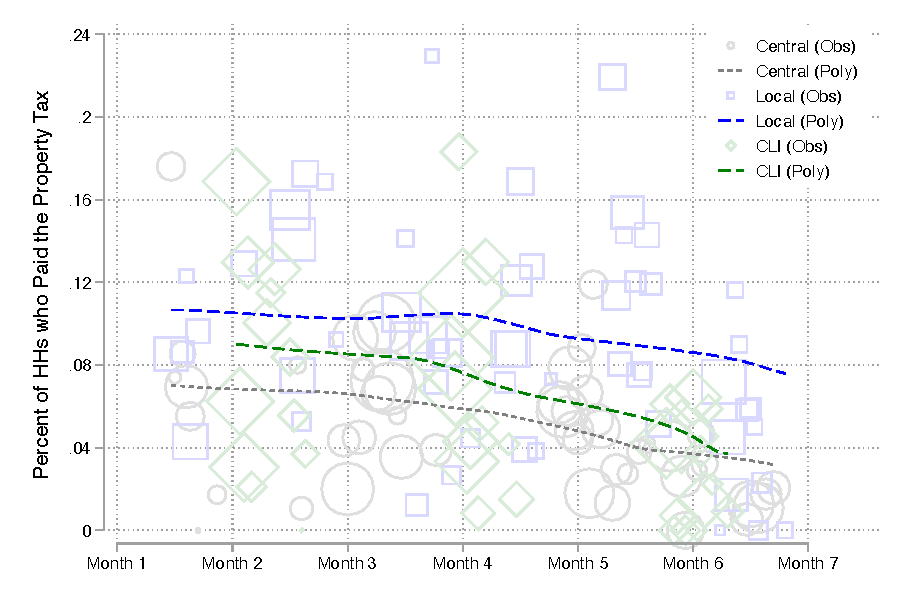
\includegraphics[scale=0.9]{Output/compliance_over_time.pdf}
}
\caption*{\footnotesize{\upshape{\textnormal{\textit{Notes}: This figure shows the decrease in compliance for Central, Local, and CLI over the 2018 tax campaign. Blue squares represent Local observations, gray circles represent Central observations, and green diamonds represent CLI observations, with size indicating number of observations.  Lines --- dashed blue for Local, dotted gray for Central, and dashed green for CLI are local linear polynomials estimated using the displayed data, separately by treatment. This figure is discussed in Section \ref{time_imbalance}.}}}}
\end{figure}

%%%%%%%%%%%%%%%%%%%%%%%%%%%%%%%%%%%%%%%%%%%%%%%%%%%%%%%%%%%%%%%%%

\subsection{Additional Exhibits for Paper Section 6 --- Main Results}

%%%%%%%%%%%%%%%%%%%%%%%%%%%%%%%%%%%%%%%%%%%%%%%%%%%%%%%%%%%%%%%%%

\begin{landscape}

%%%%%%%%%%%%%%%%%%%%%%%%%%%%%%%%%%%%%%%%%%%%%%%%%%%%%%%%%%%%%%%%%

\begin{table}[H]
\textbf{\caption{\label{Table_CvL_TaxRobust} Local v. Central Robustness: Different Approaches to Time Imbalance}}
\centering
\tiny{{
\def\sym#1{\ifmmode^{#1}\else\(^{#1}\)\fi}
\begin{tabular}{l*{7}{c}}
\hline\hline
                &\multicolumn{1}{c}{Tax Compliance}&\multicolumn{1}{c}{Tax Compliance}&\multicolumn{1}{c}{Tax Compliance}&\multicolumn{1}{c}{Tax Compliance}&\multicolumn{3}{c}{Tax Compliance}                      \\
                &\multicolumn{1}{c}{(1)}         &\multicolumn{1}{c}{(2)}         &\multicolumn{1}{c}{(3)}         &\multicolumn{1}{c}{(4)}         &\multicolumn{1}{c}{(5)}         &\multicolumn{1}{c}{(6)}         &\multicolumn{1}{c}{(7)}         \\
\hline
Local           &    0.023\sym{**} &    0.033\sym{***}&    0.033\sym{***}&    0.031\sym{***}&    0.032\sym{***}&    0.042\sym{***}&    0.032\sym{***}\\
                &  (0.008)         &  (0.007)         &  (0.007)         &  (0.007)         &  (0.007)         &  (0.007)         &  (0.008)         \\
Month FE        &       No         &       No         &       No         &       No         &      Yes         &       No         &       No         \\
House FE        &      Yes         &      Yes         &      Yes         &      Yes         &      Yes         &      Yes         &      Yes         \\
Stratum FE      &      Yes         &      Yes         &      Yes         &      Yes         &      Yes         &      Yes         &      Yes         \\
\hline
Observations    &    28872         &    27764         &    27506         &    37186         &    28872         &    25912         &    26637         \\
Clusters        &      221         &      213         &      211         &      221         &      221         &      199         &      203         \\
Mean            &     .068         &     .063         &     .064         &     .063         &     .068         &     .053         &     .068         \\
\hline\hline
\end{tabular}
}
}
\tiny{{
\def\sym#1{\ifmmode^{#1}\else\(^{#1}\)\fi}
\begin{tabular}{l*{7}{c}}
\hline\hline
                &\multicolumn{1}{c}{Tax Revenues}&\multicolumn{1}{c}{Tax Revenues}&\multicolumn{1}{c}{Tax Revenues}&\multicolumn{1}{c}{Tax Revenues}&\multicolumn{3}{c}{Tax Revenues}                        \\
                &\multicolumn{1}{c}{(1)}         &\multicolumn{1}{c}{(2)}         &\multicolumn{1}{c}{(3)}         &\multicolumn{1}{c}{(4)}         &\multicolumn{1}{c}{(5)}         &\multicolumn{1}{c}{(6)}         &\multicolumn{1}{c}{(7)}         \\
\hline
Local           &   46.362\sym{**} &   69.744\sym{***}&   69.558\sym{**} &   73.775\sym{***}&   68.695\sym{**} &   91.176\sym{***}&   77.966\sym{**} \\
                & (23.068)         & (20.695)         & (21.493)         & (18.343)         & (21.901)         & (20.199)         & (30.905)         \\
Month FE        &       No         &       No         &       No         &       No         &      Yes         &       No         &       No         \\
House FE        &      Yes         &      Yes         &      Yes         &      Yes         &      Yes         &      Yes         &      Yes         \\
Stratum FE      &      Yes         &      Yes         &      Yes         &      Yes         &      Yes         &      Yes         &      Yes         \\
\hline
Observations    &    28872         &    27370         &    27664         &    36792         &    28872         &    25912         &    26637         \\
Clusters        &      221         &      210         &      212         &      221         &      221         &      199         &      203         \\
Mean            &  192.891         &  184.394         &  185.422         &  184.394         &  192.891         &  158.855         &  192.891         \\
\hline\hline
\end{tabular}
}
}
\usebox{\tablebox}\\[1ex]
\parbox{6in}{\footnotesize \textit{Notes}: This table displays alternate approaches for addressing time imbalance in the comparison of the Local arm to the Central arm, the excluded category, as noted in Section \ref{estimation} and discussed at length in Section \ref{time_confound_appendix}. Panel A reports impacts on compliance, and Panel B reports impacts on revenues. Column 1 makes no adjustments. Column 2 includes the time period fixed effects described in Section \ref{estimation}. Column 3 includes time period fixed effects defined by selecting the median estimate among all permutations of the start date (Figure \ref{fig:shift_start_2moFE}). Column 4 implements an interaction-weighted estimator, following \cite{gibbons2018}, in which time periods defined as in Column 2 are not included as fixed effects but interacted with the treatment indicator and the estimate is the average of the coefficient on the interaction terms, weighted by the number of observations in each period. Column 5 includes one-month fixed effects. Column 6 trims the sample to periods when both treatment arms were in operation. Column 7 implements coarsened exact matching \citep{iacus2012}. All regressions include fixed effects for house type and randomization strata and cluster standard errors at the neighborhood level. We discuss these results in Section \ref{results_discussion}.}
\end{table}


\begin{table}[H]
	\textbf{\caption*{\label{Table_CvL_TaxRobust_Replicated} Table \ref{Table_CvL_TaxRobust} $\rightarrow$ Repliacted using RI Appraoch}}
	\centering
	\tiny{{
\def\sym#1{\ifmmode^{#1}\else\(^{#1}\)\fi}
\begin{tabular}{l*{7}{c}}
\toprule
                &\multicolumn{1}{c}{Tax Compliance}&\multicolumn{1}{c}{Tax Compliance}&\multicolumn{1}{c}{Tax Compliance}&\multicolumn{1}{c}{Tax Compliance}&\multicolumn{3}{c}{Tax Compliance}\\
                &\multicolumn{1}{c}{(1)}&\multicolumn{1}{c}{(2)}&\multicolumn{1}{c}{(3)}&\multicolumn{1}{c}{(4)}&\multicolumn{1}{c}{(5)}&\multicolumn{1}{c}{(6)}&\multicolumn{1}{c}{(7)}\\
                &b/p/pvalues&b/p/pvalues&b/p/pvalues&b/p/pvalues&b/p/pvalues&b/p/pvalues&b/p/pvalues\\
\midrule
Local           &0.0233105&0.0330827&0.0328438&         &0.0321948&0.0421408&0.0233105\\
                &(0.00462)&(0.00000729)&(0.0000135)&         &(0.0000143)&(4.43e-09)&(0.00462)\\
                &[0.014000]&[0.001000]&[0.001000]&         &[0.000000]&[0.000000]&[0.016000]\\
Month FE        &       No&       No&       No&       No&      Yes&       No&       No\\
House FE        &      Yes&      Yes&      Yes&      Yes&      Yes&      Yes&      Yes\\
Stratum FE      &      Yes&      Yes&      Yes&      Yes&      Yes&      Yes&      Yes\\
\midrule
Observations    &    28872&    27764&    27506&    43771&    28872&    25912&    28872\\
Clusters        &      221&      213&      211&      221&      221&      199&      221\\
Mean            &     .068&     .063&     .064&     .063&     .068&     .053&     .068\\
\bottomrule
\end{tabular}
}
}
	\tiny{{
\def\sym#1{\ifmmode^{#1}\else\(^{#1}\)\fi}
\begin{tabular}{l*{7}{c}}
\hline\hline
                &\multicolumn{1}{c}{Tax Revenues}&\multicolumn{1}{c}{Tax Revenues}&\multicolumn{1}{c}{Tax Revenues}&\multicolumn{1}{c}{Tax Revenues}&\multicolumn{3}{c}{Tax Revenues}                        \\
                &\multicolumn{1}{c}{(1)}         &\multicolumn{1}{c}{(2)}         &\multicolumn{1}{c}{(3)}         &\multicolumn{1}{c}{(4)}         &\multicolumn{1}{c}{(5)}         &\multicolumn{1}{c}{(6)}         &\multicolumn{1}{c}{(7)}         \\
\hline
Local           &   46.362\sym{**} &   69.744\sym{***}&   69.558\sym{**} &   73.775\sym{***}&   68.695\sym{**} &   91.176\sym{***}&   77.966\sym{**} \\
                & (23.068)         & (20.695)         & (21.493)         & (18.343)         & (21.901)         & (20.199)         & (30.905)         \\
Month FE        &       No         &       No         &       No         &       No         &      Yes         &       No         &       No         \\
House FE        &      Yes         &      Yes         &      Yes         &      Yes         &      Yes         &      Yes         &      Yes         \\
Stratum FE      &      Yes         &      Yes         &      Yes         &      Yes         &      Yes         &      Yes         &      Yes         \\
\hline
Observations    &    28872         &    27370         &    27664         &    36792         &    28872         &    25912         &    26637         \\
Clusters        &      221         &      210         &      212         &      221         &      221         &      199         &      203         \\
Mean            &  192.891         &  184.394         &  185.422         &  184.394         &  192.891         &  158.855         &  192.891         \\
\hline\hline
\end{tabular}
}
}
	\usebox{\tablebox}\\[1ex]
	\parbox{6in}{\footnotesize \textit{Notes}: Replicated}
\end{table}

%%%%%%%%%%%%%%%%%%%%%%%%%%%%%%%%%%%%%%%%%%%%%%%%%%%%%%%%%%%%%%%%%

\end{landscape}

%%%%%%%%%%%%%%%%%%%%%%%%%%%%%%%%%%%%%%%%%%%%%%%%%%%%%%%%%%%%%%%%%

\begin{figure}[H]
\centering{}\caption{Shifting Two-Month Fixed Effect Start Date \label{fig:shift_start_2moFE}}
\begin{tabular}{cc}
A: Local v. Central & B: Local v. Central\\
Compliance & Revenues\\
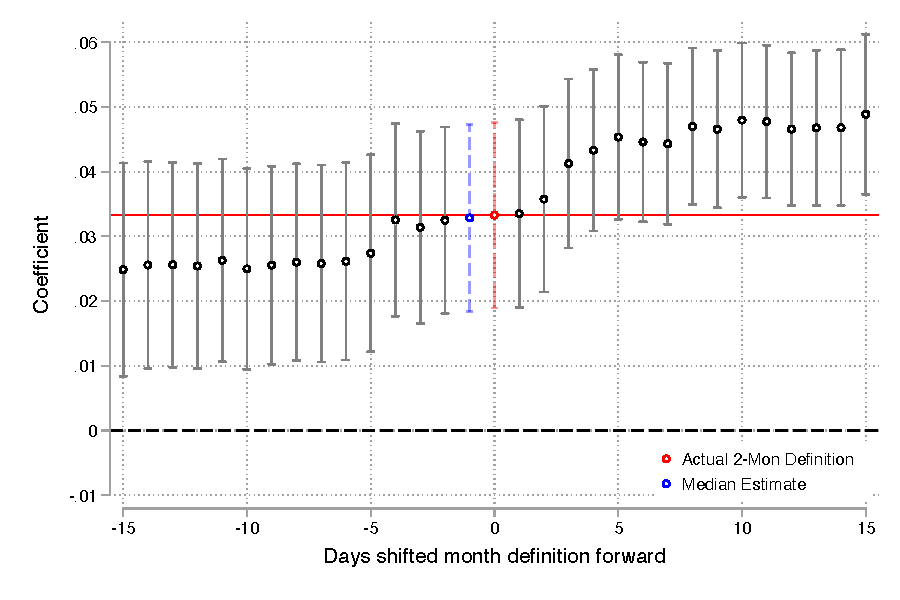
\includegraphics[scale=0.45]{Output/shiftFE_compl_CvL.pdf}&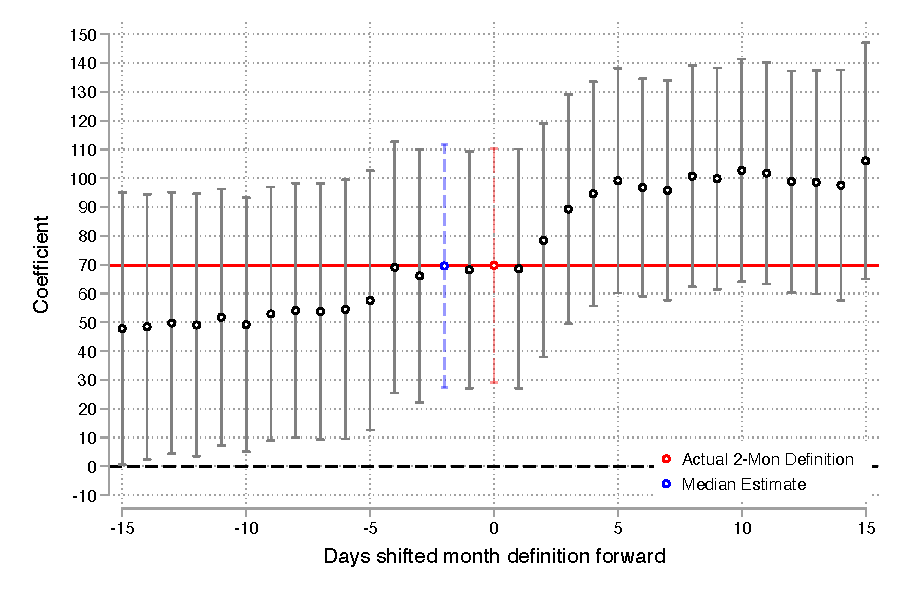
\includegraphics[scale=0.45]{Output/shiftFE_rev_CvL.pdf}\\
C: Central v. CLI & D: Central v. CLI\\
Compliance & Revenues\\
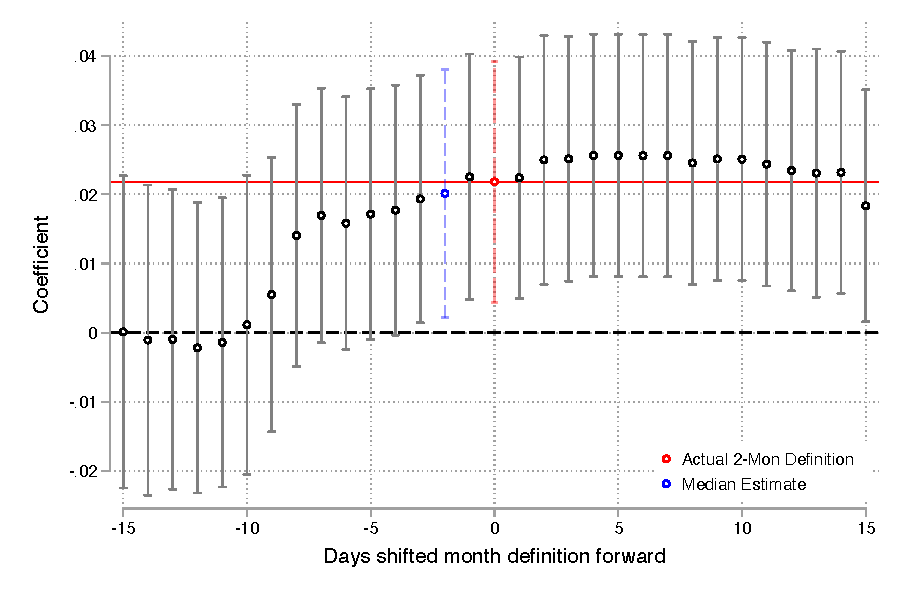
\includegraphics[scale=0.45]{Output/shiftFE_compl_CvCLI.pdf}&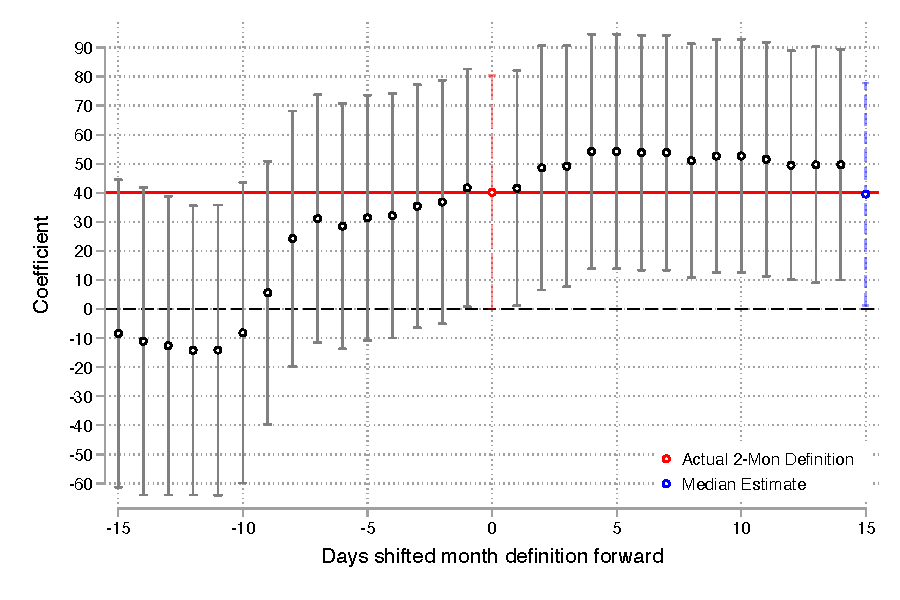
\includegraphics[scale=0.45]{Output/shiftFE_rev_CvCLI.pdf}\\
\end{tabular}
\usebox{\tablebox}\\[1ex]
\parbox{6in}{\footnotesize \emph{Notes:} This figure shows robustness to shifting the start date for defining two-month fixed effects 15 days forward and backwards from the start date in our preferred specification. Panels A and B report estimates for Local compared to Central collection for compliance and revenues, respectively.  Panels C and D report estimates for Central + Local Information (CLI) compared to Central. The long-dashed red estimate reflects the estimate using the preferred definition of time periods; the short-dashed blue estimate is the median estimate among the shifted estimates. All regressions include fixed effects for house type and randomization strata and cluster standard errors at the neighborhood level. We discuss these results in Section \ref{results_discussion} and report the median estimate in Table \ref{Table_CvL_TaxRobust}.}
\end{figure}

%%%%%%%%%%%%%%%%%%%%%%%%%%%%%%%%%%%%%%%%%%%%%%%%%%%%%%%%%%%%%%%%%

\begin{table}[H]
\textbf{\caption{\label{Table_CvL_RobustSaturated} Local v. Central Robustness: Fully-Saturated Model with Cross-Randomized Treatments}}
\centering
\tiny{{
\def\sym#1{\ifmmode^{#1}\else\(^{#1}\)\fi}
\begin{tabular}{l*{6}{c}}
\hline\hline
                &\multicolumn{1}{c}{Tax Compliance}&\multicolumn{1}{c}{Tax Compliance}&\multicolumn{1}{c}{Tax Compliance}&\multicolumn{1}{c}{Tax Compliance}&\multicolumn{1}{c}{Tax Compliance}&\multicolumn{1}{c}{Tax Compliance}\\
                &\multicolumn{1}{c}{(1)}         &\multicolumn{1}{c}{(2)}         &\multicolumn{1}{c}{(3)}         &\multicolumn{1}{c}{(4)}         &\multicolumn{1}{c}{(5)}         &\multicolumn{1}{c}{(6)}         \\
\hline
Local           &    0.033\sym{***}&    0.033\sym{***}&    0.051\sym{***}&    0.039\sym{***}&    0.036\sym{***}&    0.057\sym{***}\\
                &  (0.007)         &  (0.007)         &  (0.011)         &  (0.008)         &  (0.010)         &  (0.014)         \\
Time FE         &      Yes         &      Yes         &      Yes         &      Yes         &      Yes         &      Yes         \\
House FE        &      Yes         &      Yes         &      Yes         &      Yes         &      Yes         &      Yes         \\
Stratum FE      &      Yes         &      Yes         &      Yes         &      Yes         &      Yes         &      Yes         \\
\hline
Observations    &    27764         &    27764         &    27764         &    23618         &    23618         &    23618         \\
Clusters        &      213         &      213         &      213         &      213         &      213         &      213         \\
Mean            &     .063         &     .063         &     .063         &     .068         &     .068         &     .068         \\
\hline\hline
\end{tabular}
}
}
\small{{
\def\sym#1{\ifmmode^{#1}\else\(^{#1}\)\fi}
\begin{tabular}{l*{6}{c}}
\hline\hline
                &\multicolumn{1}{c}{Revenues}&\multicolumn{1}{c}{Revenues}&\multicolumn{1}{c}{Revenues}&\multicolumn{1}{c}{Revenues}&\multicolumn{1}{c}{Revenues}&\multicolumn{1}{c}{Revenues}\\
                &\multicolumn{1}{c}{(1)}         &\multicolumn{1}{c}{(2)}         &\multicolumn{1}{c}{(3)}         &\multicolumn{1}{c}{(4)}         &\multicolumn{1}{c}{(5)}         &\multicolumn{1}{c}{(6)}         \\
\hline
Local           &   68.855\sym{***}&   68.923\sym{***}&   75.294\sym{**} &   81.797\sym{***}&   72.674\sym{**} &   76.723\sym{**} \\
                & (20.560)         & (20.562)         & (23.838)         & (23.626)         & (22.119)         & (28.482)         \\
Time FE         &      Yes         &      Yes         &      Yes         &      Yes         &      Yes         &      Yes         \\
House FE        &      Yes         &      Yes         &      Yes         &      Yes         &      Yes         &      Yes         \\
Stratum FE      &      Yes         &      Yes         &      Yes         &      Yes         &      Yes         &      Yes         \\
\hline
Observations    &    27764         &    27764         &    27764         &    23618         &    23618         &    23618         \\
Clusters        &      213         &      213         &      213         &      213         &      213         &      213         \\
Mean            &  182.236         &  182.236         &  182.236         &  196.263         &  196.263         &  196.263         \\
\hline\hline
\end{tabular}
}
}
\usebox{\tablebox}\\[1ex]
\parbox{6in}{\footnotesize \textit{Notes}: This table reports estimates from Equation \ref{equation_cvl}, comparing property tax outcomes in Local and Central (the excluded category). The panels show the estimates from separate regressions with the outcome an indicator for compliance (Panel A) and revenues (Panel B), respectively. All regressions include fixed effects for house, time period, and randomization strata, and they cluster standard errors at the neighborhood level. Column 1 shows the preferred specification, including no additional controls.  Column 2 includes dummies for tax rate abatement groups.  Column 3 adds interactions between the abatement group dummies and the Local indicator. Column 4 includes dummies for collector bonus type.  Column 5 adds interactions between the collector bonus type dummies and the Local indicator. Column 6 includes abatement  and collector bonus dummies and interactions with the Local indicator. \cite{bergeron2019} provides details on abatement and collector bonus treatment groups. We discuss these results in Section \ref{results_discussion}.}
\end{table}


\begin{table}[H]
	\textbf{\caption*{\label{Table_CvL_RobustSaturated_R1} Table \ref{Table_CvL_RobustSaturated} $\rightarrow$ Controlling for Trust in Chief }}
	\centering
	\resizebox{16cm}{!}{{
\def\sym#1{\ifmmode^{#1}\else\(^{#1}\)\fi}
\begin{tabular}{l*{6}{c}}
\toprule
                &\multicolumn{1}{c}{Tax Compliance}&\multicolumn{1}{c}{Tax Compliance}&\multicolumn{1}{c}{Tax Compliance}&\multicolumn{1}{c}{Tax Compliance}&\multicolumn{1}{c}{Tax Compliance}&\multicolumn{1}{c}{Tax Compliance}\\
                &\multicolumn{1}{c}{(1)}         &\multicolumn{1}{c}{(2)}         &\multicolumn{1}{c}{(3)}         &\multicolumn{1}{c}{(4)}         &\multicolumn{1}{c}{(5)}         &\multicolumn{1}{c}{(6)}         \\
\midrule
Local           &    0.027\sym{*}  &    0.028\sym{*}  &    0.050         &    0.033\sym{*}  &    0.039         &    0.082\sym{*}  \\
                &  (0.062)         &  (0.060)         &  (0.115)         &  (0.073)         &  (0.219)         &  (0.095)         \\
Not very much confidence&   -0.021         &   -0.020         &   -0.021         &   -0.023         &   -0.023         &   -0.024         \\
                &  (0.428)         &  (0.436)         &  (0.412)         &  (0.498)         &  (0.497)         &  (0.471)         \\
Some confidence &    0.009         &    0.008         &    0.008         &    0.001         &    0.001         &   -0.002         \\
                &  (0.662)         &  (0.708)         &  (0.711)         &  (0.955)         &  (0.964)         &  (0.950)         \\
A lot of confidence&   -0.019         &   -0.018         &   -0.018         &   -0.024         &   -0.025         &   -0.024         \\
                &  (0.269)         &  (0.312)         &  (0.304)         &  (0.267)         &  (0.264)         &  (0.265)         \\
Time FE         &      Yes         &      Yes         &      Yes         &      Yes         &      Yes         &      Yes         \\
House FE        &      Yes         &      Yes         &      Yes         &      Yes         &      Yes         &      Yes         \\
Stratum FE      &      Yes         &      Yes         &      Yes         &      Yes         &      Yes         &      Yes         \\
\midrule
Observations    &     2231         &     2231         &     2231         &     1682         &     1682         &     1682         \\
Clusters        &      213         &      213         &      213         &      212         &      212         &      212         \\
Mean            &     .063         &     .063         &     .063         &     .068         &     .068         &     .068         \\
\bottomrule
\end{tabular}
}
}
	\resizebox{15cm}{!}{{
\def\sym#1{\ifmmode^{#1}\else\(^{#1}\)\fi}
\begin{tabular}{l*{6}{c}}
\toprule
                &\multicolumn{1}{c}{Revenues}&\multicolumn{1}{c}{Revenues}&\multicolumn{1}{c}{Revenues}&\multicolumn{1}{c}{Revenues}&\multicolumn{1}{c}{Revenues}&\multicolumn{1}{c}{Revenues}\\
                &\multicolumn{1}{c}{(1)}         &\multicolumn{1}{c}{(2)}         &\multicolumn{1}{c}{(3)}         &\multicolumn{1}{c}{(4)}         &\multicolumn{1}{c}{(5)}         &\multicolumn{1}{c}{(6)}         \\
\midrule
Local           &   56.130         &   55.117         &   86.635         &   73.178         &   77.231         &  141.846         \\
                &  (0.203)         &  (0.212)         &  (0.369)         &  (0.201)         &  (0.323)         &  (0.297)         \\
Not very much confidence&  -46.359         &  -45.050         &  -45.692         &  -66.458         &  -66.484         &  -64.635         \\
                &  (0.666)         &  (0.674)         &  (0.670)         &  (0.645)         &  (0.645)         &  (0.655)         \\
Some confidence &  -40.214         &  -41.141         &  -40.723         &  -84.037         &  -84.231         &  -84.009         \\
                &  (0.524)         &  (0.513)         &  (0.519)         &  (0.339)         &  (0.337)         &  (0.343)         \\
A lot of confidence&  -40.457         &  -38.798         &  -38.846         &  -67.791         &  -67.938         &  -63.955         \\
                &  (0.505)         &  (0.524)         &  (0.524)         &  (0.404)         &  (0.401)         &  (0.437)         \\
Time FE         &      Yes         &      Yes         &      Yes         &      Yes         &      Yes         &      Yes         \\
House FE        &      Yes         &      Yes         &      Yes         &      Yes         &      Yes         &      Yes         \\
Stratum FE      &      Yes         &      Yes         &      Yes         &      Yes         &      Yes         &      Yes         \\
\midrule
Observations    &     2231         &     2231         &     2231         &     1682         &     1682         &     1682         \\
Clusters        &      213         &      213         &      213         &      212         &      212         &      212         \\
Mean            &    182.3         &    182.3         &    182.3         &  196.246         &  196.246         &  196.246         \\
\bottomrule
\end{tabular}
}
}
	\usebox{\tablebox}\\[1ex]
	\parbox{6in}{\footnotesize \textit{Notes}: .}
\end{table}

%%%%%%%%%%%%%%%%%%%%%%%%%%%%%%%%%%%%%%%%%%%%%%%%%%%%%%%%%%%%%%%%%

\begin{table}[H]
\textbf{\caption{\label{Table_CvL_RobustControls} Local v. Central Robustness: Including Controls, Pilot Neighborhoods, Excluding Misassigned Neighborhood, and Top-Coding}}
\centering
\tiny{{
\def\sym#1{\ifmmode^{#1}\else\(^{#1}\)\fi}
\begin{tabular}{l*{6}{c}}
\hline\hline
                &\multicolumn{1}{c}{Tax Compliance}&\multicolumn{1}{c}{Tax Compliance}&\multicolumn{1}{c}{Tax Compliance}&\multicolumn{1}{c}{Tax Compliance}&\multicolumn{1}{c}{Tax Compliance}&\multicolumn{1}{c}{Tax Compliance}\\
                &\multicolumn{1}{c}{(1)}         &\multicolumn{1}{c}{(2)}         &\multicolumn{1}{c}{(3)}         &\multicolumn{1}{c}{(4)}         &\multicolumn{1}{c}{(5)}         &\multicolumn{1}{c}{(6)}         \\
\hline
Local           &    0.032\sym{***}&    0.030\sym{***}&    0.031\sym{***}&    0.031\sym{***}&    0.033\sym{***}&    0.029\sym{***}\\
                &  (0.007)         &  (0.007)         &  (0.007)         &  (0.007)         &  (0.007)         &  (0.006)         \\
Month FE        &      Yes         &      Yes         &      Yes         &      Yes         &      Yes         &      Yes         \\
House FE        &      Yes         &      Yes         &      Yes         &      Yes         &      Yes         &       No         \\
Stratum FE      &      Yes         &      Yes         &      Yes         &      Yes         &      Yes         &      Yes         \\
\hline
Observations    &    27751         &    27751         &    27751         &    28784         &    27658         &      219         \\
Clusters        &      213         &      213         &      213         &      219         &      212         &                  \\
Mean            &     .063         &     .063         &     .063         &     .064         &     .063         &     .061         \\
\hline\hline
\end{tabular}
}
}
\normalsize{{
\def\sym#1{\ifmmode^{#1}\else\(^{#1}\)\fi}
\begin{tabular}{l*{6}{c}}
\hline\hline
                &\multicolumn{1}{c}{Revenues}&\multicolumn{1}{c}{Revenues}&\multicolumn{1}{c}{Revenues}&\multicolumn{1}{c}{Revenues}&\multicolumn{1}{c}{Revenues}&\multicolumn{1}{c}{Revenues}\\
                &\multicolumn{1}{c}{(1)}         &\multicolumn{1}{c}{(2)}         &\multicolumn{1}{c}{(3)}         &\multicolumn{1}{c}{(4)}         &\multicolumn{1}{c}{(5)}         &\multicolumn{1}{c}{(6)}         \\
\hline
Local           &   65.349\sym{**} &   60.651\sym{**} &   62.026\sym{**} &   64.469\sym{**} &   68.718\sym{***}&   64.366\sym{**} \\
                & (20.531)         & (21.003)         & (20.817)         & (19.917)         & (20.486)         & (19.999)         \\
Month FE        &      Yes         &      Yes         &      Yes         &      Yes         &      Yes         &      Yes         \\
House FE        &      Yes         &      Yes         &      Yes         &      Yes         &      Yes         &       No         \\
Stratum FE      &      Yes         &      Yes         &      Yes         &      Yes         &      Yes         &      Yes         \\
\hline
Observations    &    27751         &    27751         &    27751         &    28766         &    27658         &      219         \\
Clusters        &      213         &      213         &      213         &      219         &      212         &                  \\
Mean            &    182.3         &    182.3         &    182.3         &  181.525         &    182.3         &  182.416         \\
\hline\hline
\end{tabular}
}
}
\usebox{\tablebox}\\[1ex]
\parbox{6in}{\footnotesize \textit{Notes}: This table reports estimates from Equation \ref{equation_cvl}, comparing property tax outcomes in Local and Central (the excluded category). The panels show the estimates from separate regressions with the outcome an indicator for compliance (Panel A) and revenues (Panel B), respectively. All regressions include fixed effects for house, time period, and randomization strata, and they cluster standard errors at the neighborhood level. Column 1 includes controls for age, age-squared, and gender, measured in midline survey. Column 2 adds a control for distance from schools (the one imbalanced covariate when comparing Local to Central in Table \ref{tab:balance_tests_F}). Column 3 adds controls for having any job, a salaried job, and a government job, a family member with a government job, and belonging to the majority tribe. When including controls, we replace missing values in control variables with the mean for the entire sample and include a separate dummy (for each control variable) for the value being missing. Column 4 includes pilot neighborhoods, with time period and stratum values that reflect its implementation several months before the campaign and in a remote neighborhood. Column 5 excludes the neighborhood misassigned from CXL to Local during the campaign. Column 6 displays estimates from a regression on mean outcomes at the neighborhood-level, winsorizing the top 10\% of neighborhoods, using robust standard errors, and assigning the minimum value for time period fixed effects to a neighborhood. We discuss these results in Section \ref{results_discussion}.}
\end{table}


\begin{table}[H]
	\textbf{\caption*{\label{Table_CvL_RobustControls_R1} Table \ref{Table_CvL_RobustControls} $\rightarrow$ Using Trust in Chief }}
	\centering
\resizebox{16cm}{!}{{
\def\sym#1{\ifmmode^{#1}\else\(^{#1}\)\fi}
\begin{tabular}{l*{6}{c}}
\toprule
                &\multicolumn{1}{c}{Tax Compliance}&\multicolumn{1}{c}{Tax Compliance}&\multicolumn{1}{c}{Tax Compliance}&\multicolumn{1}{c}{Tax Compliance}&\multicolumn{1}{c}{Tax Compliance}&\multicolumn{1}{c}{Tax Compliance}\\
                &\multicolumn{1}{c}{(1)}         &\multicolumn{1}{c}{(2)}         &\multicolumn{1}{c}{(3)}         &\multicolumn{1}{c}{(4)}         &\multicolumn{1}{c}{(5)}         &\multicolumn{1}{c}{(6)}         \\
\midrule
Local           &    0.027\sym{*}  &    0.023         &    0.024         &    0.027\sym{*}  &    0.028\sym{*}  &    0.030\sym{***}\\
                &  (0.064)         &  (0.116)         &  (0.107)         &  (0.062)         &  (0.061)         &  (0.000)         \\
Not very much confidence&   -0.027         &   -0.026         &   -0.027         &   -0.021         &   -0.021         &                  \\
                &  (0.297)         &  (0.309)         &  (0.294)         &  (0.427)         &  (0.415)         &                  \\
Some confidence &    0.010         &    0.009         &    0.009         &    0.009         &    0.009         &                  \\
                &  (0.644)         &  (0.654)         &  (0.650)         &  (0.665)         &  (0.680)         &                  \\
A lot of confidence&   -0.016         &   -0.016         &   -0.017         &   -0.019         &   -0.019         &                  \\
                &  (0.385)         &  (0.364)         &  (0.333)         &  (0.268)         &  (0.277)         &                  \\
trust\_chief\_mean&                  &                  &                  &                  &                  &    0.002         \\
                &                  &                  &                  &                  &                  &  (0.855)         \\
Month FE        &      Yes         &      Yes         &      Yes         &      Yes         &      Yes         &      Yes         \\
House FE        &      Yes         &      Yes         &      Yes         &      Yes         &      Yes         &       No         \\
Stratum FE      &      Yes         &      Yes         &      Yes         &      Yes         &      Yes         &      Yes         \\
\midrule
Observations    &     2231         &     2231         &     2231         &     2231         &     2225         &      213         \\
Clusters        &      213         &      213         &      213         &      213         &      212         &                  \\
Mean            &     .063         &     .063         &     .063         &     .064         &     .063         &     .061         \\
\bottomrule
\end{tabular}
}
}
	\resizebox{14cm}{!}{{
\def\sym#1{\ifmmode^{#1}\else\(^{#1}\)\fi}
\begin{tabular}{l*{6}{c}}
\toprule
                &\multicolumn{1}{c}{Revenues}&\multicolumn{1}{c}{Revenues}&\multicolumn{1}{c}{Revenues}&\multicolumn{1}{c}{Revenues}&\multicolumn{1}{c}{Revenues}&\multicolumn{1}{c}{Revenues}\\
                &\multicolumn{1}{c}{(1)}         &\multicolumn{1}{c}{(2)}         &\multicolumn{1}{c}{(3)}         &\multicolumn{1}{c}{(4)}         &\multicolumn{1}{c}{(5)}         &\multicolumn{1}{c}{(6)}         \\
\midrule
Local           &   54.920         &   54.102         &   51.380         &   56.093         &   56.614         &   68.288\sym{**} \\
                &  (0.210)         &  (0.236)         &  (0.268)         &  (0.204)         &  (0.200)         &  (0.001)         \\
Not very much confidence&  -64.581         &  -65.870         &  -70.262         &  -46.603         &  -47.866         &                  \\
                &  (0.554)         &  (0.545)         &  (0.510)         &  (0.664)         &  (0.656)         &                  \\
Some confidence &  -40.712         &  -42.402         &  -36.276         &  -40.480         &  -41.307         &                  \\
                &  (0.523)         &  (0.506)         &  (0.569)         &  (0.522)         &  (0.515)         &                  \\
A lot of confidence&  -32.345         &  -32.219         &  -29.456         &  -40.774         &  -39.984         &                  \\
                &  (0.596)         &  (0.597)         &  (0.631)         &  (0.503)         &  (0.512)         &                  \\
trust\_chief\_mean&                  &                  &                  &                  &                  &  -12.623         \\
                &                  &                  &                  &                  &                  &  (0.628)         \\
Month FE        &      Yes         &      Yes         &      Yes         &      Yes         &      Yes         &      Yes         \\
House FE        &      Yes         &      Yes         &      Yes         &      Yes         &      Yes         &       No         \\
Stratum FE      &      Yes         &      Yes         &      Yes         &      Yes         &      Yes         &      Yes         \\
\midrule
Observations    &     2231         &     2231         &     2231         &     2231         &     2225         &      213         \\
Clusters        &      213         &      213         &      213         &      213         &      212         &                  \\
Mean            &    182.3         &    182.3         &    182.3         &  181.525         &    182.3         &  182.416         \\
\bottomrule
\end{tabular}
}
}
	\usebox{\tablebox}\\[1ex]
	\parbox{6in}{\footnotesize \textit{Notes}: .}
\end{table}

%%%%%%%%%%%%%%%%%%%%%%%%%%%%%%%%%%%%%%%%%%%%%%%%%%%%%%%%%%%%%%%%%

\begin{landscape}

%%%%%%%%%%%%%%%%%%%%%%%%%%%%%%%%%%%%%%%%%%%%%%%%%%%%%%%%%%%%%%%%%

\begin{table}[H]
\textbf{\caption{Local v. Central: Controlling for Collector Characteristics \label{cvl_collector_differences_control}}}
\centering
\begin{lrbox}{\tablebox}
\scalebox{0.8}{
{
\def\sym#1{\ifmmode^{#1}\else\(^{#1}\)\fi}
\begin{tabular}{l*{9}{c}}
\hline\hline
                &\multicolumn{1}{c}{taxes\_paid}&\multicolumn{1}{c}{taxes\_paid}&\multicolumn{1}{c}{taxes\_paid}&\multicolumn{1}{c}{taxes\_paid}&\multicolumn{1}{c}{taxes\_paid}&\multicolumn{1}{c}{taxes\_paid}&\multicolumn{1}{c}{taxes\_paid}&\multicolumn{1}{c}{taxes\_paid}&\multicolumn{1}{c}{taxes\_paid}\\
\hline
Local           &   0.0331\sym{***}&   0.0378\sym{**} &   0.0374\sym{***}&   0.0435\sym{***}&   0.0340\sym{***}&   0.0338\sym{***}&   0.0328\sym{***}&   0.0358\sym{***}&   0.0456\sym{**} \\
                & (0.0072)         & (0.0166)         & (0.0073)         & (0.0081)         & (0.0078)         & (0.0085)         & (0.0091)         & (0.0082)         & (0.0207)         \\
Age             &                  &  -0.0002         &                  &                  &                  &                  &                  &                  &   0.0001         \\
                &                  & (0.0005)         &                  &                  &                  &                  &                  &                  & (0.0005)         \\
Number of possessions&                  &                  &   0.0059         &                  &                  &                  &                  &                  &   0.0058         \\
                &                  &                  & (0.0042)         &                  &                  &                  &                  &                  & (0.0048)         \\
Years of education&                  &                  &                  &   0.0032\sym{**} &                  &                  &                  &                  &   0.0032\sym{**} \\
                &                  &                  &                  & (0.0013)         &                  &                  &                  &                  & (0.0014)         \\
Trust in government (mean)&                  &                  &                  &                  &   0.0030         &                  &                  &                  &   0.0050         \\
                &                  &                  &                  &                  & (0.0049)         &                  &                  &                  & (0.0053)         \\
Taxes important &                  &                  &                  &                  &                  &  -0.0009         &                  &                  &  -0.0039         \\
                &                  &                  &                  &                  &                  & (0.0078)         &                  &                  & (0.0080)         \\
Tax ministry important&                  &                  &                  &                  &                  &                  &  -0.0000         &                  &   0.0003         \\
                &                  &                  &                  &                  &                  &                  & (0.0062)         &                  & (0.0069)         \\
Progressiveness (mean)&                  &                  &                  &                  &                  &                  &                  &   0.0052         &   0.0104         \\
                &                  &                  &                  &                  &                  &                  &                  & (0.0120)         & (0.0130)         \\
House FE        &      Yes         &      Yes         &      Yes         &      Yes         &      Yes         &      Yes         &      Yes         &      Yes         &      Yes         \\
Stratum FE      &      Yes         &      Yes         &      Yes         &      Yes         &      Yes         &      Yes         &      Yes         &      Yes         &      Yes         \\
Time FE         &      Yes         &      Yes         &      Yes         &      Yes         &      Yes         &      Yes         &      Yes         &      Yes         &      Yes         \\
\hline
\(R^{2}\)       &    0.023         &    0.023         &    0.024         &    0.025         &    0.024         &    0.024         &    0.023         &    0.024         &    0.025         \\
Observations    &    27764         &    26497         &    27453         &    27031         &    26489         &    27152         &    26361         &    27152         &    25443         \\
Clusters        &      213         &      203         &      210         &      207         &      203         &      208         &      202         &      208         &      194         \\
Mean            &     .075         &     .075         &     .075         &     .075         &     .075         &     .075         &     .075         &     .075         &     .075         \\
\hline\hline
\end{tabular}
}

}
\end{lrbox}
\usebox{\tablebox}\\[1ex]
\parbox{7.3in}{\footnotesize \textit{Notes}: This table reports estimates from Equation \ref{equation_cvl}, comparing property tax outcomes in Local and Central (the excluded category), while additionally controlling for collector characteristics for which state and chief collectors have statistically significant differences in Columns 2--8. The value of collector characteristics are those of the chief in Local and the mean of those of the assigned collectors in Central. All regressions include fixed effects for randomization strata, time periods, and cluster standard errors at the neighborhood level. We discuss these results in Section \ref{results_discussion}.}
\end{table}

%%%%%%%%%%%%%%%%%%%%%%%%%%%%%%%%%%%%%%%%%%%%%%%%%%%%%%%%%%%%%%%%%

\begin{table}[H]
\textbf{\caption{Local v. Central: Exemption Categories \label{exemptions}}}
\centerfloat
\begin{lrbox}{\tablebox}
\scalebox{0.8}{
{
\def\sym#1{\ifmmode^{#1}\else\(^{#1}\)\fi}
\begin{tabular}{l*{8}{c}}
\hline\hline
                &\multicolumn{1}{c}{Exempted}&\multicolumn{1}{c}{Enum agrees}&\multicolumn{1}{c}{Senior}&\multicolumn{1}{c}{Widow}&\multicolumn{1}{c}{Gov Pension}&\multicolumn{1}{c}{Handicap}&\multicolumn{1}{c}{Exempted}&\multicolumn{1}{c}{Exempted}\\
\hline
Local           &    0.039\sym{*}  &   -0.012         &    0.041\sym{***}&   -0.006         &    0.005         &    0.003\sym{**} &    0.041         &   -0.026         \\
                &  (0.021)         &  (0.007)         &  (0.014)         &  (0.012)         &  (0.003)         &  (0.001)         &  (0.032)         &  (0.024)         \\
t\_lXtribe\_match &                  &                  &                  &                  &                  &                  &    0.041         &                  \\
                &                  &                  &                  &                  &                  &                  &  (0.040)         &                  \\
Co-ethnic       &                  &                  &                  &                  &                  &                  &   -0.080\sym{***}&                  \\
                &                  &                  &                  &                  &                  &                  &  (0.030)         &                  \\
t\_lXknow\_eachother&                  &                  &                  &                  &                  &                  &                  &    0.067\sym{*}  \\
                &                  &                  &                  &                  &                  &                  &                  &  (0.038)         \\
Knows Colllector&                  &                  &                  &                  &                  &                  &                  &    0.064\sym{**} \\
                &                  &                  &                  &                  &                  &                  &                  &  (0.031)         \\
Time FE         &      Yes         &      Yes         &      Yes         &      Yes         &      Yes         &      Yes         &      Yes         &      Yes         \\
House FE        &      Yes         &      Yes         &      Yes         &      Yes         &      Yes         &      Yes         &      Yes         &      Yes         \\
Stratum FE      &      Yes         &      Yes         &      Yes         &      Yes         &      Yes         &      Yes         &      Yes         &      Yes         \\
\hline
\(R^{2}\)       &    0.055         &    0.020         &    0.042         &    0.029         &    0.016         &    0.006         &    0.065         &    0.064         \\
Observations    &    13772         &    13771         &    13772         &    13772         &    13772         &    13772         &     7288         &    13772         \\
Clusters        &      213         &      213         &      213         &      213         &      213         &      213         &      207         &      213         \\
Mean            &     .264         &.9560000000000001         &     .126         &     .112         &     .013         &     .004         &     .314         &     .031         \\
\hline\hline
\multicolumn{9}{l}{\footnotesize \scriptsize{Standard errors clustered by polygon. $^* p<0.1, ^{**} p<0.05, ^{***} p<0.01$.}}\\
\end{tabular}
}

}
\end{lrbox}
\usebox{\tablebox}\\[1ex]
\parbox{\wd\tablebox}{\footnotesize \emph{Notes:} This table shows differences in the exemption rates of properties by chief and state collectors. Column 1 examines treatment effects on official exemptions. Column 2 reports whether third-party evaluations of exemption status diverged with the official designation. Columns 3--6 correspond to the different exemption categories: being senior (age 65+) in Column 3, being a widow in Column 4, receiving a government pension in Column 5 and being handicapped in Column 6. Columns 7 and 8 report exemptions by treatment and coethnicity between collectors and property owners and whether the collector and property owner know one another, respectively. All regressions include randomization stratum fixed effects and house fixed effects as well as the time fixed effects described in Section \ref{estimation} and standard errors are clustered at the neighborhood-level. These results are discussed in Section \ref{results_discussion}.}
\end{table}

%%%%%%%%%%%%%%%%%%%%%%%%%%%%%%%%%%%%%%%%%%%%%%%%%%%%%%%%%%%%%%%%%

\end{landscape}

%%%%%%%%%%%%%%%%%%%%%%%%%%%%%%%%%%%%%%%%%%%%%%%%%%%%%%%%%%%%%%%%%

\clearpage

%%%%%%%%%%%%%%%%%%%%%%%%%%%%%%%%%%%%%%%%%%%%%%%%%%%%%%%%%%%%%%%%%

\begin{table}[H]
\textbf{\caption{\label{SUTVA} Local v. Central:  Awareness of Other Treatments}}
\centering
\begin{lrbox}{\tablebox}
\scalebox{0.55}{
{
\def\sym#1{\ifmmode^{#1}\else\(^{#1}\)\fi}
\begin{tabular}{l*{8}{c}}
\hline\hline
                &\multicolumn{1}{c}{Tax Compliance}&\multicolumn{1}{c}{Tax Compliance}&\multicolumn{1}{c}{Tax Compliance}&\multicolumn{5}{c}{Tax Compliance}                                                            \\
                &\multicolumn{1}{c}{(1)}         &\multicolumn{1}{c}{(2)}         &\multicolumn{1}{c}{(3)}         &\multicolumn{1}{c}{(4)}         &\multicolumn{1}{c}{(5)}         &\multicolumn{1}{c}{(6)}         &\multicolumn{1}{c}{(7)}         &\multicolumn{1}{c}{(8)}         \\
\hline
Local           &    0.033\sym{***}&    0.030\sym{**} &    0.035\sym{***}&    0.029\sym{*}  &    0.033\sym{***}&    0.033\sym{***}&    0.034\sym{**} &    0.034\sym{**} \\
                &  (0.007)         &  (0.013)         &  (0.009)         &  (0.016)         &  (0.008)         &  (0.010)         &  (0.012)         &  (0.012)         \\
t\_lXn\_other\_tmt\_strict&                  &    0.003         &                  &                  &                  &                  &                  &                  \\
                &                  &  (0.008)         &                  &                  &                  &                  &                  &                  \\
(sum) other\_tmt\_strict&    0.004         &    0.003         &                  &                  &                  &                  &                  &                  \\
                &  (0.005)         &  (0.008)         &                  &                  &                  &                  &                  &                  \\
t\_lXn\_other\_tmt\_broad&                  &                  &                  &    0.003         &                  &                  &                  &                  \\
                &                  &                  &                  &  (0.006)         &                  &                  &                  &                  \\
(sum) other\_tmt\_broad&                  &                  &   -0.001         &   -0.003         &                  &                  &                  &                  \\
                &                  &                  &  (0.004)         &  (0.005)         &                  &                  &                  &                  \\
t\_lXother\_tmt\_strict\_border&                  &                  &                  &                  &                  &   -0.002         &                  &                  \\
                &                  &                  &                  &                  &                  &  (0.030)         &                  &                  \\
(sum) other\_tmt\_strict\_border&                  &                  &                  &                  &    0.007         &    0.008         &                  &                  \\
                &                  &                  &                  &                  &  (0.015)         &  (0.029)         &                  &                  \\
t\_lXother\_tmt\_broad\_border&                  &                  &                  &                  &                  &                  &    0.004         &    0.004         \\
                &                  &                  &                  &                  &                  &                  &  (0.018)         &  (0.018)         \\
(sum) other\_tmt\_broad\_border&                  &                  &                  &                  &                  &                  &   -0.012         &   -0.012         \\
                &                  &                  &                  &                  &                  &                  &  (0.020)         &  (0.020)         \\
(max) nbr\_count &   -0.001         &   -0.001         &    0.001         &    0.001         &                  &                  &                  &                  \\
                &  (0.003)         &  (0.003)         &  (0.003)         &  (0.003)         &                  &                  &                  &                  \\
(max) border\_tot&                  &                  &                  &                  &    0.002         &    0.001         &    0.006         &    0.006         \\
                &                  &                  &                  &                  &  (0.008)         &  (0.008)         &  (0.009)         &  (0.009)         \\
Time FE         &      Yes         &      Yes         &      Yes         &      Yes         &      Yes         &      Yes         &      Yes         &      Yes         \\
House FE        &      Yes         &      Yes         &      Yes         &      Yes         &      Yes         &      Yes         &      Yes         &      Yes         \\
Stratum FE      &      Yes         &      Yes         &      Yes         &      Yes         &      Yes         &      Yes         &      Yes         &      Yes         \\
\hline
Observations    &    27764         &    27764         &    27764         &    27764         &    27764         &    27764         &    27764         &    27764         \\
Clusters        &      213         &      213         &      213         &      213         &      213         &      213         &      213         &      213         \\
Mean            &     .068         &     .068         &     .068         &     .068         &     .068         &     .068         &     .068         &     .068         \\
\hline\hline
\end{tabular}
}

}
\end{lrbox}
\usebox{\tablebox}\\[1ex]
\parbox{6in}{\footnotesize \textit{Notes}: This table analyzes potential spillovers due to awareness of other types of tax collectors working in adjacent neighborhoods. The specifications follow \cite{miguel2004} in controlling for the number of adjacent neighborhoods in different treatments (as well as the total number of adjacent neighborhoods). We evaluate two definitions of alternate treatments: the ``strict'' version codes adjacent neighborhoods as being in the alternate treatment if in Central (for a Local neighborhood) or Local (for a Central neighborhood); the ``broad'' version codes this as Central, CLI, or CXL (if Local) and Local or CXL (if Central). Due to campaign staggering across neighborhoods, we only consider exposure to treatments in adjacent neighborhoods in which collectors had already worked or were currently working, rather than neighborhoods that had been assigned to a different treatment but had not yet received tax collectors. Columns 1 and 3 report estimates of the impact of Local, controlling for the number of adjacent neighborhoods in the alternate treatment arm and total adjacent neighborhoods, for the strict and broad definitions, respectively. Columns 2 and 4 report estimates of the impact of Local collection with an interaction term for the number of adjacent neighborhoods assigned to the alternate treatment arm, controlling for the total number of adjacent neighborhoods, for strict and broad, respectively. Columns 5 and 7 report estimates of the impact of Local, controlling for length of neighborhood borders (in kilometers) shared with the alternate treatment and total length of borders, for strict and broad respectively. Columns 6 and 8 report estimates of the impact of Local collection with an interaction term for the length of neighborhood borders shared with neighborhoods assigned to the alternate treatment arm, controlling for length of neighborhood borders shared with the alternate treatment and total length of borders, for strict and broad, respectively. We include fixed effects for house type, randomization strata and time periods described in Section \ref{estimation} and cluster standard errors at the neighborhood level.  We discuss these results in Section \ref{results_discussion}.}
\end{table}

%%%%%%%%%%%%%%%%%%%%%%%%%%%%%%%%%%%%%%%%%%%%%%%%%%%%%%%%%%%%%%%%%

\begin{table}[H]
\textbf{\caption{\label{othertaxes} Local v. Central: Fiscal Externalities}}
\centering
\begin{lrbox}{\tablebox}
\scalebox{0.95}{
{\def\sym#1{\ifmmode^{#1}\else\(^{#1}\)\fi} \begin{tabular}{l*{5}{c}} \hline\hline 
& beta & SE & r2 & N & centralmean \\
Salongo (Midline) & -0.031 & 0.032 & 0.057 & 13952.000 & 0.376 \\
Salongo Hours (Midline) & -0.240 & 0.247 & 0.025 & 13568.000 & 1.659 \\
Salongo (Endline) & 0.005 & 0.028 & 0.063 & 2413.000 & 0.404 \\
Salongo Hours (Endline) & 0.459 & 0.445 & 0.051 & 2358.000 & 3.996 \\
Vehicle Tax & 0.013 & 0.008 & 0.049 & 2405.000 & 0.031 \\
Market Vendor Fee & 0.057 & 0.017 & 0.046 & 2409.000 & 0.128 \\
Business Tax & 0.008 & 0.010 & 0.044 & 2409.000 & 0.043 \\
Income Tax & 0.037 & 0.014 & 0.031 & 2406.000 & 0.095 \\
Fake Tax & 0.003 & 0.005 & 0.025 & 2387.000 & 0.014 \\
\hline\hline \end{tabular} }

}
\end{lrbox}
\usebox{\tablebox}\\[1ex]
\parbox{6in}{\footnotesize \textit{Notes}: Each row summarizes an OLS estimation of Equation \ref{equation_cvl}, comparing Local and Central, with the dependent variable noted in the first column. $\hat{\beta}$ is the coefficient on the treatment indicator, followed by the cluster-robust standard error, $R^2$, number of observations, and $\bar{x}_{Central}$ the Central group mean. In Panel A, rows 1 and 2 (3 and 4) report \emph{salongo} contributions along the extensive margin and intensive margin of hours, respectively, at midline (endline). In Panel B, the outcomes are self-reported payment of other formal taxes at endline. Obsolete tax is a poll tax, which existed in the past but does not currently exist, to test the reliability of self-reports. All regressions include fixed effects for randomization strata, and cluster standard errors at the neighborhood level. Regressions using midline data include house type fixed effects, while those using endline data do not, as discussed in Section \ref{estimation}, because this affords analysis in a larger endline sample. The number of observations varies across regressions due to (\textit{i}) outcomes being drawn from different surveys, and (\textit{ii}) non-response for specific survey questions. We discuss these results in Section \ref{salongo_discussion}.}
\end{table}

%%%%%%%%%%%%%%%%%%%%%%%%%%%%%%%%%%%%%%%%%%%%%%%%%%%%%%%%%%%%%%%%%

\begin{table}[H]
\textbf{\caption{\label{salongo} Local v. Central: Informal Labor Tax Substitution}}
\centering
\tiny{{
\def\sym#1{\ifmmode^{#1}\else\(^{#1}\)\fi}
\begin{tabular}{l*{4}{c}}
\hline\hline
                &\multicolumn{1}{c}{Salongo (Midline)}&\multicolumn{1}{c}{Salongo Amt (Midline)}&\multicolumn{1}{c}{Salongo (Endline)}&\multicolumn{1}{c}{Salongo Amt (Endline)}\\
                &\multicolumn{1}{c}{(1)}         &\multicolumn{1}{c}{(2)}         &\multicolumn{1}{c}{(3)}         &\multicolumn{1}{c}{(4)}         \\
\hline
Local           &   -0.026         &   -0.207         &    0.000         &    0.490         \\
                &  (0.032)         &  (0.254)         &  (0.030)         &  (0.454)         \\
t\_lXtaxes\_paid  &   -0.075\sym{**} &   -0.262         &   -0.051         &   -1.387         \\
                &  (0.035)         &  (0.226)         &  (0.070)         &  (1.039)         \\
taxes\_paid      &    0.061\sym{**} &   -0.128         &    0.038         &    0.757         \\
                &  (0.029)         &  (0.167)         &  (0.052)         &  (0.796)         \\
Time FE         &      Yes         &      Yes         &       No         &       No         \\
House FE        &      Yes         &      Yes         &      Yes         &      Yes         \\
Stratum FE      &      Yes         &      Yes         &      Yes         &      Yes         \\
\hline
Observations    &    13953         &    13569         &     2330         &     2278         \\
Clusters        &      206         &      205         &      221         &      221         \\
Mean            &     .372         &    1.685         &     .406         &    4.008         \\
\hline\hline
\end{tabular}
}
}
\tiny{{
\def\sym#1{\ifmmode^{#1}\else\(^{#1}\)\fi}
\begin{tabular}{l*{4}{c}}
\hline\hline
                &\multicolumn{1}{c}{Salongo (Midline)}&\multicolumn{1}{c}{Salongo Amt (Midline)}&\multicolumn{1}{c}{Salongo (Endline)}&\multicolumn{1}{c}{Salongo Amt (Endline)}\\
                &\multicolumn{1}{c}{(1)}         &\multicolumn{1}{c}{(2)}         &\multicolumn{1}{c}{(3)}         &\multicolumn{1}{c}{(4)}         \\
\hline
Local           &   -0.014         &   -0.106         &    0.022         &    1.927         \\
                &  (0.042)         &  (0.666)         &  (0.081)         &  (1.324)         \\
t\_lXpred\_compl\_dum&   -0.035         &   -0.253         &   -0.097         &   -2.186         \\
                &  (0.041)         &  (0.650)         &  (0.096)         &  (1.538)         \\
pred\_compl\_dum  &    0.090\sym{***}&    0.157         &    0.178\sym{**} &    2.651\sym{**} \\
                &  (0.023)         &  (0.664)         &  (0.077)         &  (0.941)         \\
Time FE         &      Yes         &      Yes         &       No         &       No         \\
House FE        &      Yes         &      Yes         &      Yes         &      Yes         \\
Stratum FE      &      Yes         &      Yes         &      Yes         &      Yes         \\
\hline
Observations    &     9835         &     9726         &      583         &      568         \\
Clusters        &      195         &      190         &      150         &      150         \\
Mean            &     .355         &    1.697         &     .372         &    4.382         \\
\hline\hline
\end{tabular}
}
}
\usebox{\tablebox}\\[1ex]
\parbox{6in}{\footnotesize \textit{Notes}: This table shows estimates from versions of Equation \ref{equation_cvl}, comparing the Local arm to the Central arm (excluded group), where we include an interaction with verified property tax payment (Panel A) and predicted compliance (Panel B). Predicted compliance is defined as belonging to the top 25th percentile of values for the mean of predicted ease of payment and predicted willingness to pay, generated through the exercise described in Section \ref{info_adv}. The outcome is informal labor tax (\textit{salongo}) participation as measured in the midline and endline surveys. Columns 1 and 2 report \textit{salongo} contributions along the extensive margin and intensive margin (hours contributed), respectively, at midline.  Columns 3 and 4 report the same at endline.  All regressions include fixed effects for house type and randomization strata and cluster standard errors at the neighborhood level.  Columns 1 and 2 include time period fixed effects because they analyze midline data, as discussed in Section \ref{estimation}. We discuss these results in Section \ref{salongo_discussion}.}
\end{table}

%%%%%%%%%%%%%%%%%%%%%%%%%%%%%%%%%%%%%%%%%%%%%%%%%%%%%%%%%%%%%%%%%

\begin{table}[ht]
\vspace{.5cm}
\textbf{\caption{Local v. Central: ``Total'' Tax Burden (Taxes, Bribes, Salongo)  \label{cvl_total_tax_burden}}}
\centering
\centerfloat
\begin{lrbox}{\tablebox}
\scalebox{.9}{
{
\def\sym#1{\ifmmode^{#1}\else\(^{#1}\)\fi}
\begin{tabular}{l*{4}{c}}
\hline\hline
                &\multicolumn{1}{c}{(1)}         &\multicolumn{1}{c}{(2)}         &\multicolumn{1}{c}{(3)}         &\multicolumn{1}{c}{(4)}         \\
\hline
Local           &    0.029\sym{*}  &    0.127\sym{***}&    0.033\sym{***}&    0.105\sym{**} \\
                &  (0.017)         &  (0.027)         &  (0.007)         &  (0.038)         \\
Time FE         &      Yes         &      Yes         &      Yes         &      Yes         \\
House FE        &      Yes         &      Yes         &      Yes         &      Yes         \\
Stratum FE      &      Yes         &      Yes         &      Yes         &      Yes         \\
\hline
Observations    &    27764         &    27138         &    27764         &    27138         \\
Clusters        &  213.000         &  213.000         &  213.000         &  213.000         \\
Observations    &27764.000         &27138.000         &27764.000         &27138.000         \\
Mean            &     .234         &     .045         &     .063         &     .055         \\
\hline\hline
\end{tabular}
}

}
\end{lrbox}
\usebox{\tablebox}\\[1ex]
\parbox{6.3in}{\footnotesize{\textit{Notes}: This table shows treatment effects on household payment of property taxes, bribes, and/or \textit{salongo} labor contributions. Columns 1 and 3 show the extensive margin (i.e. dummies for paying taxes or bribes, or for paying taxes, bribes, or doing \textit{salongo}). Columns 2 and 4 show the intensive margin of contributions, i.e. the total number of contributions (max = 3). These intensive-margin outcomes are standardized to facilitate interpretation of magnitudes.  }}
\vspace{.5cm}
\end{table}

%%%%%%%%%%%%%%%%%%%%%%%%%%%%%%%%%%%%%%%%%%%%%%%%%%%%%%%%%%%%%%%%%

\clearpage

%%%%%%%%%%%%%%%%%%%%%%%%%%%%%%%%%%%%%%%%%%%%%%%%%%%%%%%%%%%%%%%%%

\begin{landscape}

%%%%%%%%%%%%%%%%%%%%%%%%%%%%%%%%%%%%%%%%%%%%%%%%%%%%%%%%%%%%%%%%%

\begin{table}[H]
\textbf{\caption{Investigating Hawthorne Effects: Awareness of Monitoring and Bribe-Taking Behavior in Local \label{bribe_chief_worried_sanctions}}}
\centering
\centerfloat
\scalebox{.85}{
{
\def\sym#1{\ifmmode^{#1}\else\(^{#1}\)\fi}
\begin{tabular}{l*{3}{c}}
\hline\hline
                &\multicolumn{1}{c}{Whom did your household pay?}&\multicolumn{1}{c}{Whom did your household pay?}&\multicolumn{1}{c}{Whom did your household pay?}\\
\hline
Knows fired chiefs&   0.0009         &                  &                  \\
                & (0.0065)         &                  &                  \\
Knows 2016 campaign&                  &  -0.0055         &                  \\
                &                  & (0.0056)         &                  \\
Assigned to 2016 campaign&                  &                  &  -0.0014         \\
                &                  &                  & (0.0278)         \\
House FE        &      Yes         &      Yes         &      Yes         \\
Stratum FE      &      Yes         &      Yes         &      Yes         \\
\hline
\(R^{2}\)       &    0.017         &    0.018         &    0.017         \\
Observations    &     6393         &     6393         &     6492         \\
Clusters        &      108         &      108         &      110         \\
Mean            &     .018         &     .018         &     .018         \\
\hline\hline
\end{tabular}
}

}
\scalebox{.85}{
\tiny{{
\def\sym#1{\ifmmode^{#1}\else\(^{#1}\)\fi}
\begin{tabular}{l*{3}{c}}
\hline\hline
                &\multicolumn{1}{c}{Chief Perception of Monitoring / Punishment for Bribe-Taking}&\multicolumn{1}{c}{Chief Perception of Monitoring / Punishment for Bribe-Taking}&\multicolumn{1}{c}{Chief Perception of Monitoring / Punishment for Bribe-Taking}\\
\hline
Knows fire chiefs&  -0.4583\sym{**} &                  &                  \\
                & (0.2277)         &                  &                  \\
Knows 2016 campaign&                  &   0.0646         &                  \\
                &                  & (0.2881)         &                  \\
Nbhd in 2016 campaign&                  &                  &  -0.0371         \\
                &                  &                  & (0.2324)         \\
\hline
\(R^{2}\)       &    0.049         &    0.001         &    0.000         \\
Observations    &                  &                  &                  \\
Clusters        &                  &                  &                  \\
Mean            &     .043         &     .043         &     .043         \\
\hline\hline
\end{tabular}
}
}
}
\usebox{\tablebox}\\[1ex]
\parbox{5.8in}{\footnotesize{\textit{Notes}: This table shows correlations between baseline chief/neighborhood characteristics and outcomes related to the acceptance of bribes in Local (i.e. neighborhoods with chief tax collection). Columns 1--3 examine an outcome drawn from a survey with chiefs conducted after the 2018 tax campaign, in which chiefs were asked to estimate the probability that collectors accepting bribes during the campaign would be sanctioned. Columns 4--6 examine bribe payment reported by citizens in the midline survey. \textit{Knows deposed chiefs} and \textit{Knows 2016 campaign} come from a baseline survey conducted with chiefs, who reported whether they had ever heard of (\textit{i}) a chief being deposed, and (\textit{ii}) the 2016 property tax campaign, respectively. \textit{Nbhd in 2016 campaign} indicates neighborhoods randomly assigned to the 2016 property tax campaign, as measured in administrative data. We discuss these results in Section \ref{bribe_discussion}.}}
\vspace{.5cm}
\end{table}

%%%%%%%%%%%%%%%%%%%%%%%%%%%%%%%%%%%%%%%%%%%%%%%%%%%%%%%%%%%%%%%%%

\end{landscape}

%%%%%%%%%%%%%%%%%%%%%%%%%%%%%%%%%%%%%%%%%%%%%%%%%%%%%%%%%%%%%%%%%

\begin{table}[H]
\textbf{\caption{Heterogeneous Treatment Effects by Chief Characteristics: Bribes \label{bribe_chief_het_condensed}}}
\centering
\centerfloat
\begin{lrbox}{\tablebox}
\scalebox{.9}{
{\def\sym#1{\ifmmode^{#1}\else\(^{#1}\)\fi} \begin{tabular}{l*{8}{c}} \hline\hline 
& beta1 & SE1 & beta2 & SE2 & beta3 & SE3 & N & Depvarmean \\
Age & -0.003 & 0.004 & 0.010 & 0.006 & -0.006 & 0.005 & 12129.000 & 0.018 \\
Wealth (possessions) & -0.001 & 0.003 & 0.015 & 0.009 & -0.005 & 0.006 & 12129.000 & 0.017 \\
Years of education & 0.002 & 0.004 & -0.002 & 0.006 & 0.003 & 0.005 & 12129.000 & 0.015 \\
Minority ethnic & 0.001 & 0.004 & 0.004 & 0.009 & -0.007 & 0.005 & 11978.000 & 0.018 \\
Locality chief & 0.005 & 0.005 & -0.005 & 0.006 & 0.010 & 0.006 & 10669.000 & 0.015 \\
Chief for over 10 years & -0.001 & 0.004 & 0.005 & 0.006 & -0.004 & 0.005 & 11978.000 & 0.016 \\
Dynastic succession & 0.001 & 0.004 & -0.001 & 0.007 & -0.003 & 0.005 & 11869.000 & 0.018 \\
Remote neighborhood & 0.011 & 0.004 & -0.015 & 0.005 & 0.001 & 0.005 & 12129.000 & 0.014 \\
Customary chief & 0.003 & 0.004 & -0.002 & 0.006 & -0.017 & 0.007 & 12129.000 & 0.017 \\
Political party member & 0.008 & 0.004 & -0.019 & 0.007 & 0.010 & 0.006 & 11978.000 & 0.014 \\
Ruling party member & 0.006 & 0.004 & -0.022 & 0.009 & 0.013 & 0.008 & 11978.000 & 0.015 \\
Opposition party member & 0.003 & 0.004 & -0.014 & 0.009 & 0.002 & 0.006 & 11978.000 & 0.016 \\
Has other gov position & 0.002 & 0.004 & -0.002 & 0.007 & 0.004 & 0.006 & 11978.000 & 0.018 \\
Trust in government & 0.007 & 0.005 & -0.013 & 0.007 & 0.005 & 0.005 & 12129.000 & 0.016 \\
Trust in tax ministry & 0.007 & 0.004 & -0.015 & 0.007 & 0.008 & 0.005 & 12129.000 & 0.015 \\
View of government & 0.001 & 0.004 & 0.001 & 0.007 & -0.001 & 0.005 & 12129.000 & 0.016 \\
View of gov responsiveness & 0.002 & 0.005 & -0.000 & 0.006 & -0.004 & 0.005 & 12129.000 & 0.017 \\
View of gov integrity & 0.004 & 0.004 & -0.005 & 0.006 & 0.003 & 0.006 & 12129.000 & 0.015 \\
Knows fired chiefs & 0.001 & 0.005 & -0.000 & 0.007 & 0.006 & 0.005 & 11978.000 & 0.017 \\
Knows 2016 campaign & 0.004 & 0.006 & -0.004 & 0.008 & -0.002 & 0.005 & 11869.000 & 0.014 \\
Neighborhood in 2016 campaign & 0.003 & 0.004 & -0.002 & 0.006 & 0.013 & 0.017 & 12077.000 & 0.015 \\
Trusted by citizens & 0.004 & 0.005 & -0.005 & 0.007 & 0.006 & 0.005 & 12129.000 & 0.017 \\
Accessible to citizens & 0.007 & 0.005 & -0.010 & 0.007 & 0.002 & 0.005 & 12129.000 & 0.016 \\
Active in chief role & 0.003 & 0.005 & -0.003 & 0.007 & 0.003 & 0.005 & 12129.000 & 0.018 \\
\hline\hline \end{tabular} }

}
\end{lrbox}
\usebox{\tablebox}\\[1ex]
\parbox{6.3in}{\footnotesize{\textit{Notes}: This table shows heterogeneous treatment effects by a range of chief characteristics measured before the tax campaign. Specifically, each row summarizes the results from estimating the equation $y_{ijkt}={\beta_0}+\beta_1 Local_{jkt} + \beta_2 Local_{jkt} * Z^{Chief}_{jk} + \beta_3 Z^{Chief}_{jk} + \alpha_k+ \theta_t + \varepsilon_{ijkt} $,  where $Z^{Chief}_{jk}$ indicates the corresponding characteristic of the neighborhood chief shown in the first cell of each row. $y_{ijkt}$ is bribe payment, $\alpha_{k}$ are stratum fixed effects, and $\theta_t$ are time fixed effects. Standard errors are clustered at the neighborhood level (213 in total). All chief characteristics are 0-1 to maximize power for estimating heterogeneous treatment effects. Continuous variables are transformed into indicators to report above-median values of the characteristics (denoted by $>p50$). We discuss these results in Section \ref{bribe_discussion}.}}
\end{table}

%%%%%%%%%%%%%%%%%%%%%%%%%%%%%%%%%%%%%%%%%%%%%%%%%%%%%%%%%%%%%%%%%

\begin{table}[H]
\vspace{.5cm}
\textbf{\caption{The Counterfactual to Chief Bribe Collection: Predicting Chief Bribe Payers in Central \label{c_predbribepayers}}}
\centering
\centerfloat
{
\def\sym#1{\ifmmode^{#1}\else\(^{#1}\)\fi}
\begin{tabular}{l*{3}{c}}
\hline\hline
                &\multicolumn{1}{c}{Compliance}&\multicolumn{1}{c}{Compliance}&\multicolumn{1}{c}{Bribes (Endline)}\\
                &\multicolumn{1}{c}{(1)}         &\multicolumn{1}{c}{(2)}         &\multicolumn{1}{c}{(3)}         \\
\hline
Predicted Bribe Payer&    0.013         &    0.032         &   -0.000         \\
                &  (0.024)         &  (0.054)         &  (0.018)         \\
Stratum FE      &      Yes         &      Yes         &      Yes         \\
\hline
Observations    &      847         &      329         &      414         \\
Clusters        &      109         &       95         &      102         \\
Mean            &     .089         &     .089         &     .013         \\
\hline\hline
\end{tabular}
}
\\
{
\def\sym#1{\ifmmode^{#1}\else\(^{#1}\)\fi}
\begin{tabular}{l*{3}{c}}
\hline\hline
                &\multicolumn{1}{c}{Compliance}&\multicolumn{1}{c}{Compliance}&\multicolumn{1}{c}{Bribes (Endline)}\\
                &\multicolumn{1}{c}{(1)}         &\multicolumn{1}{c}{(2)}         &\multicolumn{1}{c}{(3)}         \\
\hline
Predicted Bribe Payer&    0.069\sym{*}  &    0.146\sym{*}  &   -0.020\sym{**} \\
                &  (0.041)         &  (0.085)         &  (0.008)         \\
Stratum FE      &      Yes         &      Yes         &      Yes         \\
\hline
Observations    &      847         &      329         &      414         \\
Clusters        &      109         &       95         &      102         \\
Mean            &     .086         &     .086         &     .016         \\
\hline\hline
\end{tabular}
}

\usebox{\tablebox}\\[1ex]
\parbox{6.3in}{\footnotesize{\textit{Notes}: This table provides evidence on the counterfactual of the increase in bribes in Local relative to Central. Specifically, it shows correlations between predicted chief bribe payment and tax and bribe payments in the Central treatment arm. Predicted bribe payment is constructed by regressing bribe payment (at endline) in Local on baseline household and property characteristics, retaining the variables with significant coefficients, and using these variables to predict bribe payment (at endline) in the Central treatment arm. This exercise simulates the likely bribe payers if Central neighborhoods had in fact been assigned to Local. The variables used in the final prediction exercise include: age of property owner, whether a family member of household members works for the government, whether the household possesses a radio, trust in the provincial government, whether the respondent knows the neighborhood chief, has the chief's phone number, and attends the same church as the chief. The Predicted Bribe Payer variable is an indicator for the predicted value being greater than the 75th (Panel A) or 90th percentile (Panel B). Tax compliance is measured using administrative tax data, post-registration visits using the midline survey, and bribe payment using the endline survey (our preferred measure using a local code for bribes, discussed in Section \ref{bribe_discussion}).  All regressions include fixed effects for randomization strata and cluster standard errors at the neighborhood level. Column 2 restricts the sample to households that received visits from tax collectors after registration. The number of observations for bribe outcomes is smaller than the full endline sample because this variable was only collected among households who reported at least one visit from tax collectors after property registration. We discuss these results in Section \ref{bribe_discussion}.}}
\vspace{.5cm}
\end{table}

%%%%%%%%%%%%%%%%%%%%%%%%%%%%%%%%%%%%%%%%%%%%%%%%%%%%%%%%%%%%%%%%%

\subsection{Additional Exhibits for Paper Section 7 --- Mechanisms}

%%%%%%%%%%%%%%%%%%%%%%%%%%%%%%%%%%%%%%%%%%%%%%%%%%%%%%%%%%%%%%%%%

\begin{table}[H]
%\vspace*{-1cm}
\textbf{\caption{\label{Table_CvL_Visits_NoHouseFE_edited} Local v. Central: Tax Visits --- No House Fixed Effects}}
\centering
\begin{lrbox}{\tablebox}
\small{{
\def\sym#1{\ifmmode^{#1}\else\(^{#1}\)\fi}
\begin{tabular}{l*{4}{c}}
\hline\hline
                &\multicolumn{1}{c}{Visited Post Carto}&\multicolumn{1}{c}{Visits Post Carto}&\multicolumn{1}{c}{Visited Other Contact}&\multicolumn{1}{c}{Visits Other Contact}\\
                &\multicolumn{1}{c}{(1)}         &\multicolumn{1}{c}{(2)}         &\multicolumn{1}{c}{(3)}         &\multicolumn{1}{c}{(4)}         \\
\hline
Local           &   -0.008         &    0.016         &    0.008         &    0.019         \\
                &  (0.026)         &  (0.046)         &  (0.007)         &  (0.013)         \\
Month FE        &      Yes         &      Yes         &      Yes         &      Yes         \\
Stratum FE      &      Yes         &      Yes         &      Yes         &      Yes         \\
\hline
Observations    &    18162         &    18151         &     3513         &     3513         \\
Clusters        &      209         &      209         &      206         &      206         \\
Mean            &     .417         &     .552         &     .025         &     .039         \\
\hline\hline
\end{tabular}
}
}
\end{lrbox}
\usebox{\tablebox}\\[1ex]
\parbox{6in}{\footnotesize \textit{Notes}: This table reports estimates from Equation \ref{equation_cvl}, comparing the tax visits collectors made after registration in Local and Central (the excluded category). All regressions include fixed effects for randomization strata and time periods described in Section \ref{estimation}, and cluster standard errors at the neighborhood level. Columns 1 and 2 report differences in tax visits by collectors --- after the registration visit --- by the extensive and intensive margins, respectively. Columns 3 and 4 report differences in other contact with collectors outside of the tax campaign, as reported by citizens, by the intensive and extensive margins, respectively. We discuss these results in Section \ref{visits_discussion}.}
\end{table}

%%%%%%%%%%%%%%%%%%%%%%%%%%%%%%%%%%%%%%%%%%%%%%%%%%%%%%%%%%%%%%%%%

\clearpage

%%%%%%%%%%%%%%%%%%%%%%%%%%%%%%%%%%%%%%%%%%%%%%%%%%%%%%%%%%%%%%%%%

\begin{landscape}

%%%%%%%%%%%%%%%%%%%%%%%%%%%%%%%%%%%%%%%%%%%%%%%%%%%%%%%%%%%%%%%%%

\begin{table}[H]
\textbf{\caption{\label{Table_CvCLI_TaxRobust} Central v. Central + Local Information Robustness: Different Approaches to Time Imbalance}}
\centering
\tiny{{
\def\sym#1{\ifmmode^{#1}\else\(^{#1}\)\fi}
\begin{tabular}{l*{7}{c}}
\hline\hline
                &\multicolumn{1}{c}{Tax Compliance}&\multicolumn{1}{c}{Tax Compliance}&\multicolumn{1}{c}{Tax Compliance}&\multicolumn{1}{c}{Tax Compliance}&\multicolumn{3}{c}{Tax Compliance}                      \\
                &\multicolumn{1}{c}{(1)}         &\multicolumn{1}{c}{(2)}         &\multicolumn{1}{c}{(3)}         &\multicolumn{1}{c}{(4)}         &\multicolumn{1}{c}{(5)}         &\multicolumn{1}{c}{(6)}         &\multicolumn{1}{c}{(7)}         \\
\hline
Central Plus Local Info&   -0.001         &    0.024\sym{**} &    0.019\sym{**} &   -0.004         &    0.024\sym{**} &    0.019\sym{**} &    0.041\sym{**} \\
                &  (0.011)         &  (0.009)         &  (0.009)         &  (0.008)         &  (0.010)         &  (0.009)         &  (0.016)         \\
Month FE        &       No         &       No         &       No         &       No         &      Yes         &       No         &       No         \\
House FE        &      Yes         &      Yes         &      Yes         &      Yes         &      Yes         &      Yes         &      Yes         \\
Stratum FE      &      Yes         &      Yes         &      Yes         &      Yes         &      Yes         &      Yes         &      Yes         \\
\hline
Observations    &    23911         &    20636         &    19767         &    32754         &    23911         &    18834         &     8575         \\
Clusters        &      190         &      165         &      161         &      190         &      190         &      150         &       72         \\
Mean            &     .068         &     .051         &     .057         &     .051         &     .068         &     .055         &     .024         \\
\hline\hline
\end{tabular}
}
}
\tiny{{
\def\sym#1{\ifmmode^{#1}\else\(^{#1}\)\fi}
\begin{tabular}{l*{7}{c}}
\hline\hline
                &\multicolumn{1}{c}{Tax Revenues}&\multicolumn{1}{c}{Tax Revenues}&\multicolumn{1}{c}{Tax Revenues}&\multicolumn{1}{c}{Tax Revenues}&\multicolumn{3}{c}{Tax Revenues}                        \\
                &\multicolumn{1}{c}{(1)}         &\multicolumn{1}{c}{(2)}         &\multicolumn{1}{c}{(3)}         &\multicolumn{1}{c}{(4)}         &\multicolumn{1}{c}{(5)}         &\multicolumn{1}{c}{(6)}         &\multicolumn{1}{c}{(7)}         \\
\hline
Central Plus Local Info&  -10.315         &   40.178\sym{*}  &   39.558\sym{**} &  -30.749         &   57.325\sym{**} &   37.204\sym{*}  &   52.277         \\
                & (26.089)         & (20.481)         & (19.509)         & (21.816)         & (20.830)         & (20.452)         & (34.337)         \\
Month FE        &       No         &       No         &       No         &       No         &      Yes         &       No         &       No         \\
House FE        &      Yes         &      Yes         &      Yes         &      Yes         &      Yes         &      Yes         &      Yes         \\
Stratum FE      &      Yes         &      Yes         &      Yes         &      Yes         &      Yes         &      Yes         &      Yes         \\
\hline
Observations    &    23911         &    20176         &    20507         &    31963         &    23911         &    18834         &     8575         \\
Clusters        &      190         &      162         &      160         &      190         &      190         &      150         &       72         \\
Mean            &  192.891         &  155.747         &  138.945         &  155.747         &  192.891         &  156.774         &   61.224         \\
\hline\hline
\end{tabular}
}
}
\usebox{\tablebox}\\[1ex]
\parbox{6in}{\footnotesize \textit{Notes}: This table displays alternate approaches for addressing time imbalance in the comparison of the Central + Local Information (CLI) arm to the Central arm, the excluded category. Panel A reports impacts on compliance, and Panel B reports impacts on revenues. Column 1 makes no adjustments. Column 2 includes the time period fixed effects described in Section \ref{estimation}. Column 3 includes time period fixed effects defined by selecting the median estimate among all permutations of the start date (Figure \ref{fig:shift_start_2moFE}). Column 4 implements an interaction-weighted estimator, following \cite{gibbons2018}, in which time periods defined as in Column 2 are not included as fixed effects but interacted with the treatment indicator and the estimate is the weighted average of the coefficient on the interaction terms, weighted by the number of observations in each period. Column 5 includes one-month fixed effects.  Column 6 trims the sample to periods when both treatment arms are in operation.  Column 7 implements coarsened exact matching \citep{iacus2012}. All regressions include fixed effects for house type and randomization strata and cluster standard errors at the neighborhood level. We discuss these results in Section \ref{cli_discussion}.}
\end{table}

%%%%%%%%%%%%%%%%%%%%%%%%%%%%%%%%%%%%%%%%%%%%%%%%%%%%%%%%%%%%%%%%%

\end{landscape}

%%%%%%%%%%%%%%%%%%%%%%%%%%%%%%%%%%%%%%%%%%%%%%%%%%%%%%%%%%%%%%%%%

\begin{table}[H]
\textbf{\caption{\label{Table_CvCLI_RobustControls} Central v. Central + Local Information Robustness: Controlling for Imbalanced Midline Covariates}}
\centering

\tiny{{
\def\sym#1{\ifmmode^{#1}\else\(^{#1}\)\fi}
\begin{tabular}{l*{6}{c}}
\hline\hline
                &\multicolumn{1}{c}{Tax Compliance}&\multicolumn{5}{c}{Tax Amount}                                                                \\
                &\multicolumn{1}{c}{(1)}         &\multicolumn{1}{c}{(2)}         &\multicolumn{1}{c}{(3)}         &\multicolumn{1}{c}{(4)}         &\multicolumn{1}{c}{(5)}         &\multicolumn{1}{c}{(6)}         \\
\hline
Central Plus Local Info&    0.024\sym{**} &   52.263\sym{**} &   -0.008         &   -0.021         &    0.021         &    0.030\sym{**} \\
                &  (0.011)         & (25.449)         &  (0.034)         &  (0.055)         &  (0.016)         &  (0.011)         \\
Local           &                  &                  &                  &                  &                  &    0.065\sym{***}\\
                &                  &                  &                  &                  &                  &  (0.009)         \\
Time FE         &      Yes         &      Yes         &      Yes         &      Yes         &      Yes         &      Yes         \\
House FE        &      Yes         &      Yes         &      Yes         &      Yes         &      Yes         &      Yes         \\
Stratum FE      &      Yes         &      Yes         &      Yes         &      Yes         &      Yes         &      Yes         \\
\hline
Observations    &    10064         &    10064         &    10051         &    10048         &     3864         &    16436         \\
Clusters        &      155         &      155         &      155         &      155         &      150         &      253         \\
Mean            &     .059         &  159.808         &     .393         &      .51         &       .1         &     .059         \\
CLIvC\_p         &                  &                  &                  &                  &                  &.0024771616937258         \\
\hline\hline
\end{tabular}
}
}
\tiny{{
\def\sym#1{\ifmmode^{#1}\else\(^{#1}\)\fi}
\begin{tabular}{l*{6}{c}}
\hline\hline
                &\multicolumn{1}{c}{Tax Compliance}&\multicolumn{5}{c}{Tax Amount}                                                                \\
                &\multicolumn{1}{c}{(1)}         &\multicolumn{1}{c}{(2)}         &\multicolumn{1}{c}{(3)}         &\multicolumn{1}{c}{(4)}         &\multicolumn{1}{c}{(5)}         &\multicolumn{1}{c}{(6)}         \\
\hline
Central Plus Local Info&    0.024\sym{**} &   24.241         &   -0.018         &   -0.029         &    0.027\sym{*}  &    0.023\sym{**} \\
                &  (0.009)         & (23.476)         &  (0.028)         &  (0.044)         &  (0.014)         &  (0.009)         \\
Local           &                  &                  &                  &                  &                  &    0.045\sym{***}\\
                &                  &                  &                  &                  &                  &  (0.007)         \\
Month FE        &      Yes         &      Yes         &      Yes         &      Yes         &      Yes         &      Yes         \\
Stratum FE      &      Yes         &      Yes         &      Yes         &      Yes         &      Yes         &      Yes         \\
\hline
Observations    &    20629         &    20629         &    13879         &    13872         &     5281         &    33731         \\
Clusters        &      165         &      165         &      163         &      163         &      161         &      267         \\
Mean            &     .051         &  150.714         &     .387         &     .497         &     .097         &     .052         \\
CLIvC\_p         &                  &                  &                  &                  &                  &.0130796014417039         \\
\hline\hline
\end{tabular}
}
}
\usebox{\tablebox}\\[1ex]
\parbox{6in}{\footnotesize \textit{Notes}: This table compares the Central + Local Information (CLI) arm to the Central arm, the excluded category, controlling for the characteristics imbalanced at midline --- sex of property owner, whether property owner is salaried, and distance to state buildings and market --- as shown in Table \ref{tab:balance_tests_F} (Panel A) and excluding house type fixed effects (Panel B). Columns 1, 5, and 6 report impacts on compliance. Column 2 reports impacts on revenues. Columns 3 and 4 report differences in tax visits by collectors after registration by the extensive and intensive margins, respectively. All regressions include fixed effects randomization strata and time periods, and cluster standard errors at the neighborhood level. Column 5 restricts to the subsample of properties that received any tax visits after registration. Column 6 includes a dummy for the Local treatment in the regression. The bottom row reports the $p$-value from a test for equality between the CLI and Local. We discuss these results in Section \ref{cli_discussion}.}
\end{table}

%%%%%%%%%%%%%%%%%%%%%%%%%%%%%%%%%%%%%%%%%%%%%%%%%%%%%%%%%%%%%%%%%

\begin{landscape}

%%%%%%%%%%%%%%%%%%%%%%%%%%%%%%%%%%%%%%%%%%%%%%%%%%%%%%%%%%%%%%%%%

\begin{table}[H]
\textbf{\caption{Local v. Central + Local Information: Heterogeneous Treatment Effects by Owner Present at Registration \label{present_sensi}}}
\centering
\centerfloat
\begin{lrbox}{\tablebox}
\scalebox{.85}{
{
\def\sym#1{\ifmmode^{#1}\else\(^{#1}\)\fi}
\begin{tabular}{l*{4}{c}}
\hline\hline
                &\multicolumn{1}{c}{Taxes Paid}&\multicolumn{1}{c}{Taxes Paid}&\multicolumn{1}{c}{Taxes Paid}&\multicolumn{1}{c}{Taxes Paid}\\
                &\multicolumn{1}{c}{(1)}         &\multicolumn{1}{c}{(2)}         &\multicolumn{1}{c}{(3)}         &\multicolumn{1}{c}{(4)}         \\
\hline
Local           &    0.021\sym{**} &    0.027\sym{**} &    0.028\sym{**} &    0.029\sym{**} \\
                &  (0.009)         &  (0.009)         &  (0.009)         &  (0.009)         \\
t\_lXpresent\_sensi&    0.001         &    0.005         &    0.005         &    0.014         \\
                &  (0.009)         &  (0.009)         &  (0.009)         &  (0.010)         \\
IS THERE AN ADULT WHO LIVES ON THE COMPOUND PRESENT RIGHT NOW TO RECEIVE THE INF&    0.039\sym{***}&    0.033\sym{***}&    0.035\sym{***}&    0.051\sym{***}\\
                &  (0.007)         &  (0.006)         &  (0.007)         &  (0.008)         \\
Time FE         &       No         &      Yes         &      Yes         &      Yes         \\
House FE        &       No         &       No         &      Yes         &      Yes         \\
Stratum FE      &      Yes         &      Yes         &      Yes         &      Yes         \\
\hline
Observations    &    28875         &    27767         &    27767         &    23805         \\
Clusters        &      221         &      213         &      213         &      213         \\
Mean            &     .036         &     .035         &     .035         &     .035         \\
\hline\hline
\end{tabular}
}

}
\end{lrbox}
\usebox{\tablebox}\\[1ex]
\parbox{6.3in}{\footnotesize{\textit{Notes}: This table reports estimates from Equation \ref{equation_cvl}, comparing property tax compliance in Local and Central (the excluded category), where we include an interaction with an indicator for the owner of the property being present at registration. All regressions include fixed effects for randomization strata and cluster standard errors at the neighborhood level. Column 1 regressions do not include time period fixed effects described in Section \ref{estimation}, while those in other columns include them. Regressions in Columns 1--2 do not include house fixed effects while Column 3 includes them. Regressions in Column 4 exclude exempt properties. The data include all properties registered by tax collectors merged with the government's property tax database. We discuss these results in Section \ref{cli_discussion}.}}
\end{table}

%%%%%%%%%%%%%%%%%%%%%%%%%%%%%%%%%%%%%%%%%%%%%%%%%%%%%%%%%%%%%%%%%

\end{landscape}

%%%%%%%%%%%%%%%%%%%%%%%%%%%%%%%%%%%%%%%%%%%%%%%%%%%%%%%%%%%%%%%%%

\begin{table}[H]
\textbf{\caption{The Value of Chiefs' Information --- No House Fixed Effects \label{validation_cli_control_NoHouseFE}}}
\centering
\centerfloat
\tiny{{
\def\sym#1{\ifmmode^{#1}\else\(^{#1}\)\fi}
\begin{tabular}{l*{8}{c}}
\hline\hline
                &\multicolumn{1}{c}{Visited Post Carto}&\multicolumn{1}{c}{Compliance}&\multicolumn{1}{c}{Visited Post Carto}&\multicolumn{1}{c}{Compliance}&\multicolumn{1}{c}{Compliance}&\multicolumn{1}{c}{Visited Post Carto}&\multicolumn{1}{c}{Compliance}&\multicolumn{1}{c}{Visited Post Carto}\\
                &\multicolumn{1}{c}{(1)}         &\multicolumn{1}{c}{(2)}         &\multicolumn{1}{c}{(3)}         &\multicolumn{1}{c}{(4)}         &\multicolumn{1}{c}{(5)}         &\multicolumn{1}{c}{(6)}         &\multicolumn{1}{c}{(7)}         &\multicolumn{1}{c}{(8)}         \\
\hline
Ease of payment &    0.046\sym{***}&    0.055\sym{***}&    0.029\sym{**} &    0.043\sym{***}&                  &                  &                  &                  \\
                &  (0.012)         &  (0.007)         &  (0.014)         &  (0.008)         &                  &                  &                  &                  \\
Predicted Ease of payment&                  &                  &                  &                  &    0.054\sym{**} &    0.045\sym{***}&    0.013         &    0.040\sym{***}\\
                &                  &                  &                  &                  &  (0.017)         &  (0.012)         &  (0.017)         &  (0.007)         \\
Wall quality    &                  &                  &    0.027\sym{**} &    0.017\sym{**} &    0.017\sym{*}  &    0.008         &    0.021\sym{**} &    0.011\sym{**} \\
                &                  &                  &  (0.012)         &  (0.007)         &  (0.010)         &  (0.006)         &  (0.010)         &  (0.004)         \\
Roof quality    &                  &                  &    0.005         &    0.000         &    0.003         &   -0.004         &    0.018\sym{**} &   -0.010         \\
                &                  &                  &  (0.006)         &  (0.002)         &  (0.006)         &  (0.004)         &  (0.008)         &  (0.006)         \\
Erosion threat  &                  &                  &    0.017         &   -0.003         &    0.002         &   -0.007         &   -0.000         &   -0.005         \\
                &                  &                  &  (0.011)         &  (0.004)         &  (0.011)         &  (0.007)         &  (0.010)         &  (0.004)         \\
Stratum FE      &      Yes         &      Yes         &      Yes         &      Yes         &      Yes         &      Yes         &      Yes         &      Yes         \\
\hline
Observations    &     5574         &     8135         &     4551         &     5150         &     5748         &     5763         &     4998         &     5004         \\
Clusters        &       79         &       80         &       66         &       66         &                  &                  &                  &                  \\
Mean            &     .376         &     .072         &     .352         &     .065         &                  &                  &                  &                  \\
\hline\hline
\end{tabular}
}
}
\tiny{{
\def\sym#1{\ifmmode^{#1}\else\(^{#1}\)\fi}
\begin{tabular}{l*{8}{c}}
\hline\hline
                &\multicolumn{1}{c}{Visited Post Carto}&\multicolumn{1}{c}{Compliance}&\multicolumn{1}{c}{Visited Post Carto}&\multicolumn{1}{c}{Compliance}&\multicolumn{1}{c}{Visited Post Carto}&\multicolumn{1}{c}{Compliance}&\multicolumn{1}{c}{Visited Post Carto}&\multicolumn{1}{c}{Compliance}\\
                &\multicolumn{1}{c}{(1)}         &\multicolumn{1}{c}{(2)}         &\multicolumn{1}{c}{(3)}         &\multicolumn{1}{c}{(4)}         &\multicolumn{1}{c}{(5)}         &\multicolumn{1}{c}{(6)}         &\multicolumn{1}{c}{(7)}         &\multicolumn{1}{c}{(8)}         \\
\hline
Willingness     &    0.035\sym{**} &    0.037\sym{***}&    0.033\sym{**} &    0.038\sym{***}&                  &                  &                  &                  \\
                &  (0.011)         &  (0.007)         &  (0.012)         &  (0.008)         &                  &                  &                  &                  \\
Predicted Willingness to pay&                  &                  &                  &                  &    0.045\sym{**} &    0.036\sym{***}&    0.007         &    0.032\sym{***}\\
                &                  &                  &                  &                  &  (0.016)         &  (0.010)         &  (0.015)         &  (0.009)         \\
Wall quality    &                  &                  &    0.025\sym{*}  &    0.017\sym{**} &    0.018\sym{*}  &    0.009         &    0.021\sym{**} &    0.011\sym{**} \\
                &                  &                  &  (0.013)         &  (0.008)         &  (0.009)         &  (0.006)         &  (0.010)         &  (0.005)         \\
Roof quality    &                  &                  &    0.011         &    0.001         &    0.004         &   -0.003         &    0.018\sym{**} &   -0.010         \\
                &                  &                  &  (0.008)         &  (0.002)         &  (0.006)         &  (0.004)         &  (0.008)         &  (0.006)         \\
Erosion threat  &                  &                  &    0.016         &   -0.004         &    0.002         &   -0.006         &   -0.000         &   -0.005         \\
                &                  &                  &  (0.012)         &  (0.005)         &  (0.011)         &  (0.007)         &  (0.010)         &  (0.005)         \\
Stratum FE      &      Yes         &      Yes         &      Yes         &      Yes         &      Yes         &      Yes         &      Yes         &      Yes         \\
\hline
Observations    &     3933         &     5521         &     3929         &     4461         &     5748         &     5763         &     4998         &     5004         \\
Clusters        &       50         &       50         &       50         &       50         &                  &                  &                  &                  \\
Mean            &     .357         &     .062         &     .357         &     .066         &                  &                  &                  &                  \\
Clusters2       &                  &                  &                  &                  &                  &                  &                  &                  \\
Mean2           &                  &                  &                  &                  &                  &                  &                  &                  \\
\hline\hline
\end{tabular}
}
}
\usebox{\tablebox}\\[1ex]
\parbox{6.3in}{\footnotesize \textit{Notes}: This table explores the extent to which chiefs' recommendations in Central + Local Information (CLI) predict tax visits after registration and tax payment, while excluding house fixed effects as a robustness check. Columns 1--5 show correlations in CLI between chiefs' recommendations and outcomes.  Columns 6--9 report correlations between predicted propensity measures described in Section \ref{info_adv} and outcomes in the Local (Columns 6 and 7) and the Central (Columns 8 and 9) arms.  Columns 1, 3, 6, and 8 show correlations between propensity and visits; Columns 2, 4, 5, 7, and 9 show correlations between propensity and compliance.  Column 5 shows correlations with compliance conditional on receiving a visit after registration. All regressions include randomization stratum fixed effects and cluster standard errors at the neighborhood level.  Columns 3, 4, and 6--8 include controls for visible household characteristics. We discuss these results in Section \ref{predictiveness_discussion}.}
\end{table}

%%%%%%%%%%%%%%%%%%%%%%%%%%%%%%%%%%%%%%%%%%%%%%%%%%%%%%%%%%%%%%%%%

\begin{table}[H]
\vspace{.5cm}
\textbf{\caption{The Value of Chiefs' Information --- Comparing Treatments \label{clipredict_interacted_eop_wtp}}}
\centering
\centerfloat
\tiny{{
\def\sym#1{\ifmmode^{#1}\else\(^{#1}\)\fi}
\begin{tabular}{l*{4}{c}}
\hline\hline
                &\multicolumn{1}{c}{Visited}&\multicolumn{1}{c}{Compliance}&\multicolumn{1}{c}{Visited}&\multicolumn{1}{c}{Compliance}\\
                &\multicolumn{1}{c}{(1)}         &\multicolumn{1}{c}{(2)}         &\multicolumn{1}{c}{(3)}         &\multicolumn{1}{c}{(4)}         \\
\hline
combine\_pay\_ease&    0.016         &    0.024\sym{**} &    0.037\sym{*}  &    0.038\sym{**} \\
                &  (0.020)         &  (0.009)         &  (0.021)         &  (0.011)         \\
t\_cliXcombine\_pay\_ease&    0.081\sym{**} &    0.028\sym{**} &    0.059\sym{*}  &    0.011         \\
                &  (0.037)         &  (0.012)         &  (0.030)         &  (0.015)         \\
Central with Info&   -0.061\sym{*}  &   -0.002         &   -0.084\sym{**} &   -0.047\sym{**} \\
                &  (0.034)         &  (0.012)         &  (0.033)         &  (0.016)         \\
t\_lXcombine\_pay\_ease&                  &                  &                  &                  \\
                &                  &                  &                  &                  \\
Local           &                  &                  &                  &                  \\
                &                  &                  &                  &                  \\
Wall quality    &    0.027\sym{**} &    0.020\sym{***}&    0.009         &    0.018\sym{**} \\
                &  (0.009)         &  (0.005)         &  (0.008)         &  (0.005)         \\
Roof quality    &    0.009         &   -0.004         &    0.005         &    0.000         \\
                &  (0.005)         &  (0.003)         &  (0.005)         &  (0.003)         \\
Erosion threat  &    0.003         &   -0.003         &   -0.002         &   -0.011\sym{**} \\
                &  (0.009)         &  (0.004)         &  (0.009)         &  (0.004)         \\
House FE        &      Yes         &      Yes         &      Yes         &      Yes         \\
Stratum FE      &      Yes         &      Yes         &      Yes         &      Yes         \\
\hline
Observations    &     8396         &     8407         &     8556         &     8575         \\
Clusters        &      139         &      139         &      144         &      144         \\
Mean            &     .413         &     .061         &     .449         &     .112         \\
\hline\hline
\end{tabular}
}
}\\
\tiny{{
\def\sym#1{\ifmmode^{#1}\else\(^{#1}\)\fi}
\begin{tabular}{l*{4}{c}}
\hline\hline
                &\multicolumn{1}{c}{Visited}&\multicolumn{1}{c}{Compliance}&\multicolumn{1}{c}{Visited}&\multicolumn{1}{c}{Compliance}\\
                &\multicolumn{1}{c}{(1)}         &\multicolumn{1}{c}{(2)}         &\multicolumn{1}{c}{(3)}         &\multicolumn{1}{c}{(4)}         \\
\hline
combine\_willingness&    0.025         &    0.026\sym{**} &    0.033         &    0.025\sym{**} \\
                &  (0.021)         &  (0.008)         &  (0.020)         &  (0.010)         \\
t\_cliXcombine\_willingness&    0.027         &    0.013         &    0.036         &    0.021         \\
                &  (0.041)         &  (0.011)         &  (0.029)         &  (0.014)         \\
Central with Info&   -0.031         &    0.006         &   -0.079\sym{*}  &   -0.059\sym{**} \\
                &  (0.044)         &  (0.017)         &  (0.042)         &  (0.018)         \\
t\_lXcombine\_willingness&                  &                  &                  &                  \\
                &                  &                  &                  &                  \\
Local           &                  &                  &                  &                  \\
                &                  &                  &                  &                  \\
Wall quality    &    0.029\sym{***}&    0.021\sym{***}&    0.009         &    0.018\sym{**} \\
                &  (0.008)         &  (0.005)         &  (0.008)         &  (0.005)         \\
Roof quality    &    0.009\sym{*}  &   -0.004         &    0.005         &    0.000         \\
                &  (0.005)         &  (0.003)         &  (0.005)         &  (0.003)         \\
Erosion threat  &    0.005         &   -0.002         &   -0.000         &   -0.011\sym{**} \\
                &  (0.009)         &  (0.004)         &  (0.009)         &  (0.004)         \\
House FE        &      Yes         &      Yes         &      Yes         &      Yes         \\
Stratum FE      &      Yes         &      Yes         &      Yes         &      Yes         \\
\hline
Observations    &     8396         &     8407         &     8556         &     8575         \\
Clusters        &      139         &      139         &      144         &      144         \\
Mean            &     .413         &     .061         &     .449         &     .112         \\
Clusters2       &                  &                  &                  &                  \\
Mean2           &                  &                  &                  &                  \\
\hline\hline
\end{tabular}
}
}
\usebox{\tablebox}\\[1ex]
\parbox{6.3in}{\footnotesize{\textit{Notes}: This table explores the extent to which the content of chiefs' recommendations in Central + Local Information (CLI) predict tax visits after registration and tax payment differentially across treatments. Columns 1--2 compare CLI to Central, regressing outcomes of receiving a post-registration visit and paying the tax, respectively, on the predicted ease of payment measure (Panel A) and willingness to pay measure (Panel B) described in Section \ref{predictiveness_discussion}, an indicator for the CLI treatment arm, and their interaction.  Columns 3--4 repeat the same exercise comparing CLI to Local. All regressions include house type and randomization stratum fixed effects, controls for observable household characteristics (wall quality, roof quality, and erosion threat), and cluster standard errors at the neighborhood level. We discuss these results in Section \ref{predictiveness_discussion}}}
\vspace{.5cm}
\end{table}

%%%%%%%%%%%%%%%%%%%%%%%%%%%%%%%%%%%%%%%%%%%%%%%%%%%%%%%%%%%%%%%%%

\begin{figure}[H]
\textbf{\caption{Tax Visits and Compliance by Chief Knowledge of Citizens \label{chief_knowl_by_tmt}}}
\centering
\begin{tabular}{cc}
\\
A: Local -- Tax Visits & B: Local -- Compliance    \\
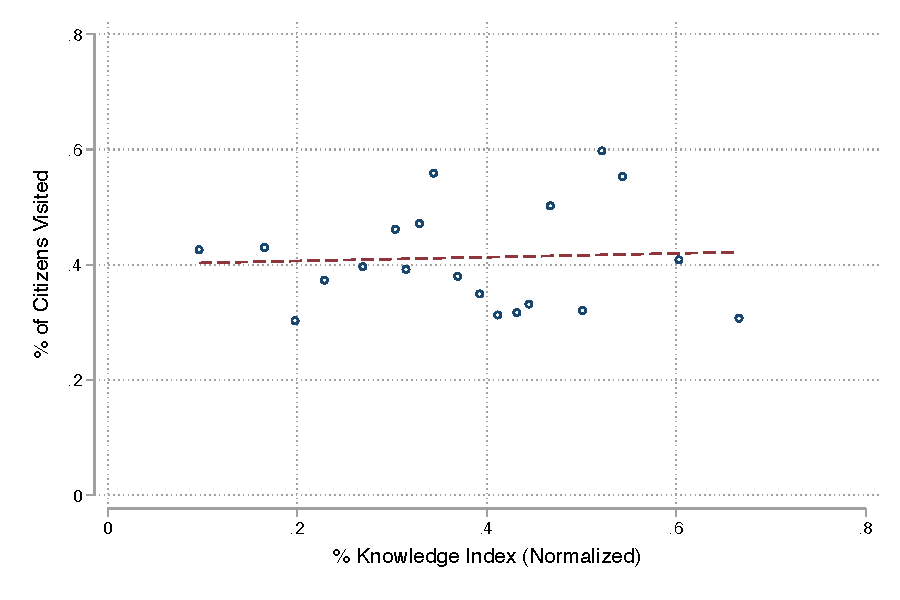
\includegraphics[scale=0.5]{Output/visits_chefknowindex_L_binned.pdf} & 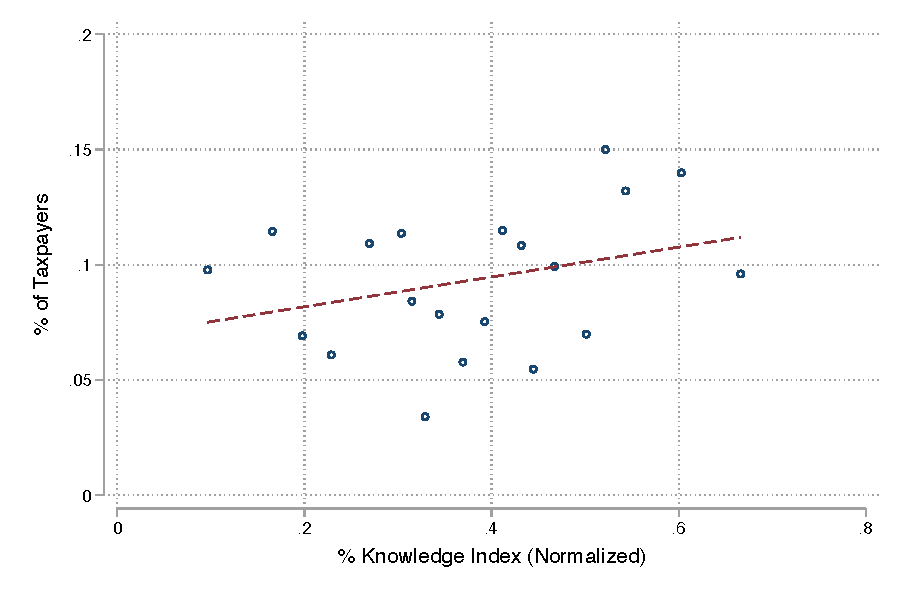
\includegraphics[scale=0.5]{Output/taxes_paid_chefknowindex_L_binned.pdf}\\
C: Central + Info --- Tax Visits & D:  Central + Info --- Compliance    \\
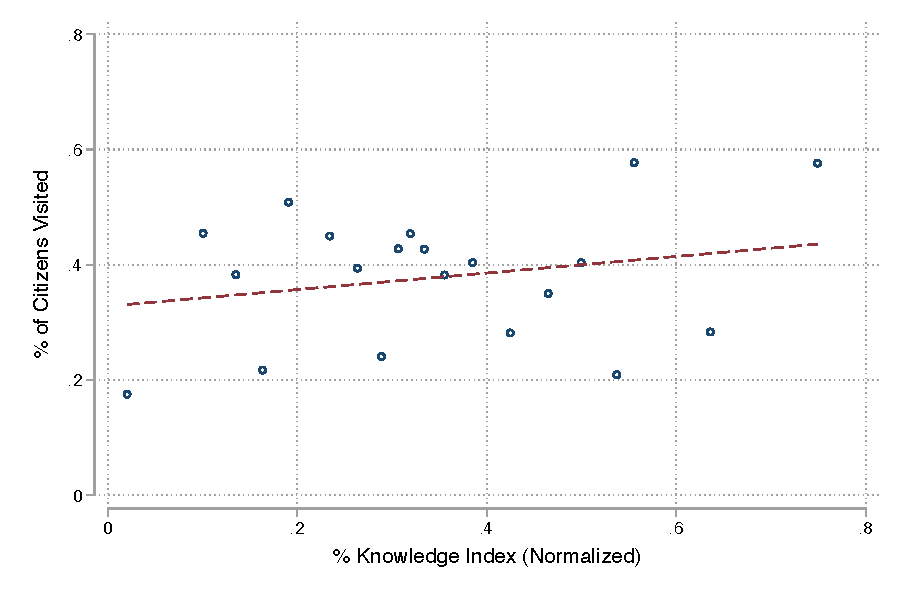
\includegraphics[scale=0.5]{Output/visits_chefknowindex_CwI_binned.pdf} & 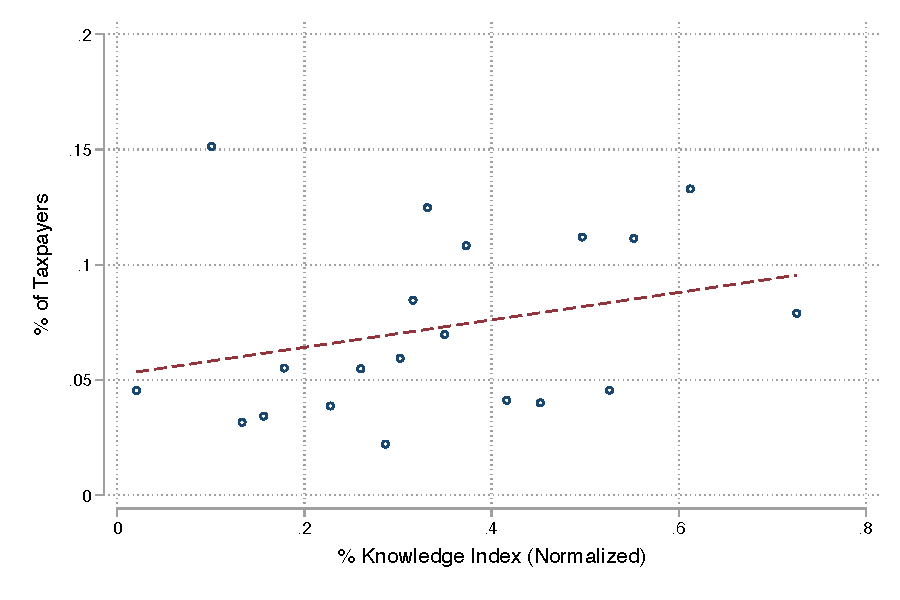
\includegraphics[scale=0.5]{Output/taxes_paid_chefknowindex_CwI_binned.pdf}\\
E: Central --- Tax Visits & F:  Central --- Compliance    \\
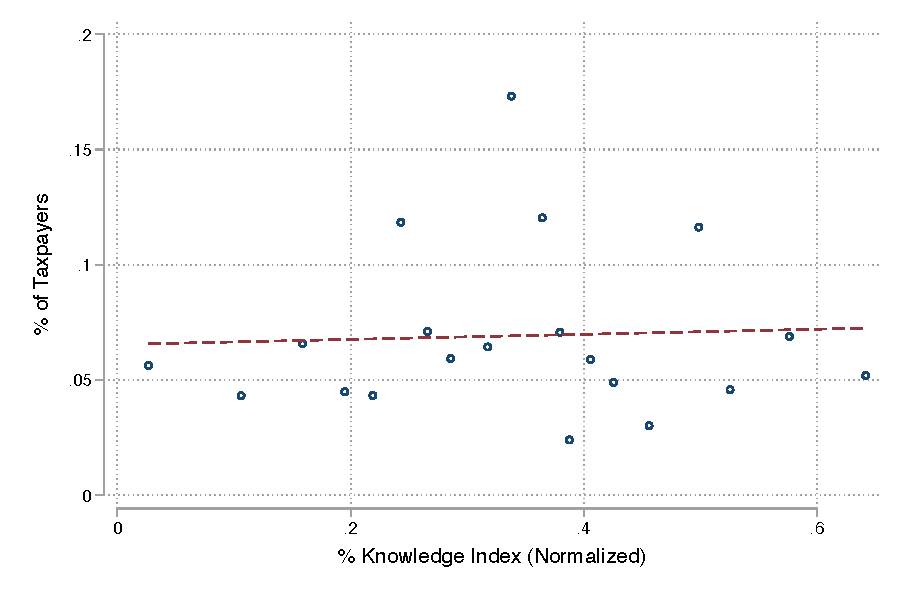
\includegraphics[scale=0.5]{Output/taxes_paid_chefknowindex_C_binned.pdf} & 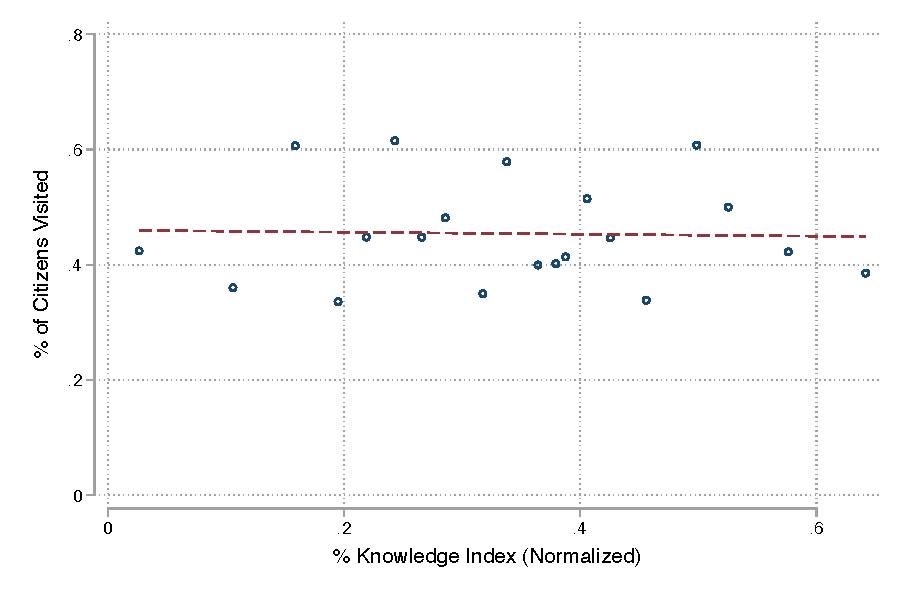
\includegraphics[scale=0.5]{Output//visits_chefknowindex_C_binned.pdf}\\

\end{tabular}
\caption*{\footnotesize{\upshape{\textnormal{\textit{Notes}: This figure shows the relationship between chiefs' knowledge of the inhabitants of the neighborhood and (\textit{i}) the percent of property owners who received a tax visit after registration (Panels A, C, and E), and (\textit{ii}) the level of tax compliance (Panels B, D, and F). Chiefs' knowledge of the inhabitants of the neighborhood is measured by the percentage of correct answers when asked to provide the name, education level, and occupation of a randomly selected group property owners. We show these relationships for neighborhoods assigned to Local in Panels A and B as well as neighborhoods assigned to CLI and Central tax collection in Panels C and D, and E and F, respectively. Table \ref{chief_knowl_by_tmt_table} analyzes these relationships in a regression framework. We discuss these results in Section \ref{predictiveness_discussion}.}}}}
\end{figure}

%%%%%%%%%%%%%%%%%%%%%%%%%%%%%%%%%%%%%%%%%%%%%%%%%%%%%%%%%%%%%%%%%

\begin{table}[ht]
\textbf{\caption{\label{chief_knowl_by_tmt_table} Tax Visits and Compliance by Chief Knowledge of Citizens}}
\centerfloat
\begin{lrbox}{\tablebox}
\resizebox{16cm}{!}{
{
\def\sym#1{\ifmmode^{#1}\else\(^{#1}\)\fi}
\begin{tabular}{l*{6}{c}}
\hline\hline
                &\multicolumn{2}{c}{CLI}              &\multicolumn{2}{c}{Central}          &\multicolumn{2}{c}{Local}            \\
                &\multicolumn{1}{c}{(1)}         &\multicolumn{1}{c}{(2)}         &\multicolumn{1}{c}{(3)}         &\multicolumn{1}{c}{(4)}         &\multicolumn{1}{c}{(5)}         &\multicolumn{1}{c}{(6)}         \\
\hline
Chief Info Above Median&    0.010         &    0.028\sym{*}  &   -0.020         &   -0.007         &   -0.016         &    0.024\sym{*}  \\
                &  (0.043)         &  (0.017)         &  (0.041)         &  (0.012)         &  (0.034)         &  (0.012)         \\
\hline
Observations    &       79         &       80         &      110         &      110         &      111         &      111         \\
Clusters        &                  &                  &                  &                  &                  &                  \\
Mean            &     .377         &     .073         &     .454         &     .069         &     .412         &     .093         \\
\hline\hline
\end{tabular}
}

}
\end{lrbox}
\usebox{\tablebox}\\[1ex]
\parbox{6in}{\footnotesize \textit{Notes}: This table shows the relationship between city chiefs' knowledge of the inhabitants of the neighborhood and (\textit{i}) the percent of property owners who received a tax visit after registration (Columns 1, 3, and 5), and (\textit{ii}) the level of tax compliance (Columns 2, 4, and 6). Chiefs' knowledge of the inhabitants of the neighborhood is measured by the percentage of correct answers when asked to provide the name, education level, and occupation of a randomly selected group property owners. We show these relationships for neighborhoods assigned to (\textit{i}) Central (Columns 1--2), where state collectors did not consult with chiefs --- a placebo check --- (\textit{ii}) Central + Local Information (Columns 3--4), where state collectors did consult with chiefs, and (\textit{iii}) Local (Columns 5--6), where chiefs themselves collected taxes. We discuss these results in Section \ref{predictiveness_discussion}.}
\end{table}


\begin{table}[ht]
	\textbf{\caption*{\label{chief_knowl_by_tmt_tableR1} Table \ref{chief_knowl_by_tmt_table} Controlling for Chiefs Characteristics }}
	\centerfloat
	\begin{lrbox}{\tablebox}
		\resizebox{16cm}{!}{
			{
\def\sym#1{\ifmmode^{#1}\else\(^{#1}\)\fi}
\begin{tabular}{l*{6}{c}}
\hline\hline
                &\multicolumn{2}{c}{CLI}              &\multicolumn{2}{c}{Central}          &\multicolumn{2}{c}{Local}            \\
                &\multicolumn{1}{c}{(1)}         &\multicolumn{1}{c}{(2)}         &\multicolumn{1}{c}{(3)}         &\multicolumn{1}{c}{(4)}         &\multicolumn{1}{c}{(5)}         &\multicolumn{1}{c}{(6)}         \\
\hline
Chief Info Above Median&   -0.011         &    0.040\sym{**} &   -0.037         &   -0.004         &   -0.007         &    0.019         \\
                &  (0.048)         &  (0.019)         &  (0.045)         &  (0.013)         &  (0.036)         &  (0.013)         \\
\hline
Observations    &       78         &       79         &      109         &      109         &      107         &      107         \\
Clusters        &                  &                  &                  &                  &                  &                  \\
Mean            &     .377         &     .073         &     .454         &     .069         &     .412         &     .093         \\
\hline\hline
\end{tabular}
}

		}
	\end{lrbox}
	\usebox{\tablebox}\\[1ex]
	\parbox{6in}{\footnotesize \textit{Notes}: \ref{predictiveness_discussion}.}
\end{table}

%%%%%%%%%%%%%%%%%%%%%%%%%%%%%%%%%%%%%%%%%%%%%%%%%%%%%%%%%%%%%%%%%

\begin{table}[ht]
\textbf{\caption{\label{dist_DGRKOC} Collector Outcomes as a Function of Distance to their Own Neighborhoods}}
\centerfloat
\begin{lrbox}{\tablebox}
\resizebox{16cm}{!}{
{
\def\sym#1{\ifmmode^{#1}\else\(^{#1}\)\fi}
\begin{tabular}{l*{4}{c}}
\hline\hline
                &\multicolumn{1}{c}{taxes\_paid}&\multicolumn{1}{c}{taxes\_paid\_amt}&\multicolumn{1}{c}{taxes\_paid}&\multicolumn{1}{c}{taxes\_paid\_amt}\\
\hline
Dist. btw collectors home and nbhd&   -0.006\sym{***}&  -12.584\sym{**} &                  &                  \\
                &  (0.002)         &  (5.754)         &                  &                  \\
dist\_chief      &                  &                  &   -0.005         &    3.071         \\
                &                  &                  &  (0.019)         & (62.236)         \\
Time FE         &      Yes         &      Yes         &      Yes         &      Yes         \\
House FE        &      Yes         &      Yes         &      Yes         &      Yes         \\
\hline
\(R^{2}\)       &    0.014         &    0.023         &    0.005         &    0.016         \\
Observations    &    22398         &    22398         &    13880         &    13880         \\
Clusters        &      183         &      183         &      107         &      107         \\
Mean            &     .066         &  172.966         &     .094         &  251.686         \\
\hline\hline
\end{tabular}
}

}
\end{lrbox}
\usebox{\tablebox}\\[1ex]
\parbox{6in}{\footnotesize \textit{Notes}: This table estimates the relationship between tax compliance (Columns 1 and 3) or tax revenue (Columns 2 and 4) and the distance between collectors' houses and the neighborhoods in which they worked. We estimate this relationship for state collectors in Central and CLI by calculating the average distance for the two randomly assigned collectors (Columns 1 and 2). The relationship for chief collectors is reported in Columns 3 and 4 for completeness, though there is little variation for chief collectors who hailed from the neighborhoods in which they taxed.  All regressions include house type and randomization stratum fixed effects as well as the time fixed effects described in Section \ref{estimation}. We cluster standard errors at the neighborhood level. We discuss these results in Section \ref{predictiveness_discussion}.}
\end{table}


\begin{table}[ht]
	\textbf{\caption*{\label{dist_DGRKOC_R1} Table \ref{dist_DGRKOC} Controlling for Chiefs characterics}}
	\centerfloat
	\begin{lrbox}{\tablebox}
		\resizebox{16cm}{!}{
			{
\def\sym#1{\ifmmode^{#1}\else\(^{#1}\)\fi}
\begin{tabular}{l*{4}{c}}
\hline\hline
                &\multicolumn{1}{c}{taxes\_paid}&\multicolumn{1}{c}{taxes\_paid\_amt}&\multicolumn{1}{c}{taxes\_paid}&\multicolumn{1}{c}{taxes\_paid\_amt}\\
\hline
Dist. btw collectors home and nbhd&   -0.006\sym{***}&  -12.278\sym{**} &                  &                  \\
                &  (0.002)         &  (5.589)         &                  &                  \\
age\_chef\_hi     &    0.015         &   38.920         &   -0.005         &   25.614         \\
                &  (0.012)         & (30.759)         &  (0.011)         & (37.341)         \\
possessions\_nb\_chef\_hi&    0.013         &   13.153         &   -0.005         &   -0.248         \\
                &  (0.010)         & (22.304)         &  (0.016)         & (45.926)         \\
educ\_yrs\_chef\_hi&    0.009         &   28.732         &    0.020         &   62.831\sym{*}  \\
                &  (0.012)         & (28.116)         &  (0.013)         & (33.699)         \\
remoteness\_hi   &   -0.001         &   -9.362         &   -0.013         &  -26.856         \\
                &  (0.010)         & (23.041)         &  (0.010)         & (33.593)         \\
chef\_trust\_gov\_hi&    0.007         &   19.678         &    0.024         &   39.274         \\
                &  (0.013)         & (30.402)         &  (0.017)         & (61.218)         \\
chef\_trust\_dgrkoc\_hi&   -0.006         &  -25.117         &   -0.010         &  -11.339         \\
                &  (0.014)         & (34.612)         &  (0.019)         & (63.643)         \\
col\_view\_gov\_gen\_hi&    0.009         &   27.188         &   -0.013         &  -59.569         \\
                &  (0.010)         & (23.828)         &  (0.013)         & (39.205)         \\
col\_view\_gov\_nbhd\_hi&   -0.016         &  -46.145\sym{*}  &   -0.008         &  -12.123         \\
                &  (0.011)         & (27.343)         &  (0.010)         & (28.364)         \\
col\_gov\_integrity\_hi&    0.004         &    7.135         &   -0.036\sym{***}& -106.379\sym{***}\\
                &  (0.009)         & (23.120)         &  (0.012)         & (34.219)         \\
tmt\_2016        &   -0.006         &   -9.141         &    0.006         &   39.548         \\
                &  (0.009)         & (24.386)         &  (0.011)         & (33.103)         \\
Was another member of your family the chef of this jurisdiction here before you?&    0.028         &   85.748\sym{*}  &   -0.003         &  -24.579         \\
                &  (0.018)         & (44.780)         &  (0.016)         & (39.792)         \\
chef\_tenure\_hi  &    0.002         &   16.035         &    0.025\sym{**} &   41.525         \\
                &  (0.012)         & (31.099)         &  (0.012)         & (37.404)         \\
dist\_chief      &                  &                  &   -0.010         &  -14.726         \\
                &                  &                  &  (0.018)         & (61.124)         \\
Time FE         &      Yes         &      Yes         &      Yes         &      Yes         \\
House FE        &      Yes         &      Yes         &      Yes         &      Yes         \\
\hline
\(R^{2}\)       &    0.017         &    0.026         &    0.012         &    0.021         \\
Observations    &    22200         &    22200         &    13602         &    13602         \\
Clusters        &      181         &      181         &      105         &      105         \\
Mean            &     .066         &  172.257         &     .095         &  251.066         \\
\hline\hline
\end{tabular}
}

		}
	\end{lrbox}
	\usebox{\tablebox}\\[1ex]
	\parbox{6in}{\footnotesize \textit{Notes}: \ref{predictiveness_discussion}.}
\end{table}
%%%%%%%%%%%%%%%%%%%%%%%%%%%%%%%%%%%%%%%%%%%%%%%%%%%%%%%%%%%%%%%%%

\clearpage

%%%%%%%%%%%%%%%%%%%%%%%%%%%%%%%%%%%%%%%%%%%%%%%%%%%%%%%%%%%%%%%%%

\begin{table}[ht]
\textbf{\caption{\label{CvsL_collector_close} Local v. Central: State Collectors Working Near their Homes}}
\centerfloat
{
\def\sym#1{\ifmmode^{#1}\else\(^{#1}\)\fi}
\begin{tabular}{l*{4}{c}}
\hline\hline
                &\multicolumn{1}{c}{taxes\_paid}&\multicolumn{1}{c}{taxes\_paid\_amt}&\multicolumn{1}{c}{taxes\_paid}&\multicolumn{1}{c}{taxes\_paid\_amt}\\
\hline
Local           &    0.027\sym{**} &   63.062\sym{**} &    0.034\sym{***}&   66.977\sym{***}\\
                &  (0.012)         & (31.702)         &  (0.009)         & (24.605)         \\
Time FE         &      Yes         &      Yes         &      Yes         &      Yes         \\
House FE        &      Yes         &      Yes         &      Yes         &      Yes         \\
\hline
\(R^{2}\)       &    0.007         &    0.017         &    0.010         &    0.022         \\
Observations    &    17225         &    17225         &    24635         &    24635         \\
Clusters        &      142         &      142         &      199         &      199         \\
Mean            &     .069         &  202.237         &     .062         &  176.298         \\
\hline\hline
\end{tabular}
}
\\
{
\def\sym#1{\ifmmode^{#1}\else\(^{#1}\)\fi}
\begin{tabular}{l*{4}{c}}
\hline\hline
                &\multicolumn{1}{c}{taxes\_paid}&\multicolumn{1}{c}{taxes\_paid\_amt}&\multicolumn{1}{c}{taxes\_paid}&\multicolumn{1}{c}{taxes\_paid\_amt}\\
\hline
Local           &    0.031\sym{**} &   73.158\sym{**} &    0.038\sym{***}&   86.362\sym{***}\\
                &  (0.013)         & (33.833)         &  (0.007)         & (18.763)         \\
Time FE         &      Yes         &      Yes         &      Yes         &      Yes         \\
House FE        &      Yes         &      Yes         &      Yes         &      Yes         \\
\hline
\(R^{2}\)       &    0.008         &    0.018         &    0.011         &    0.022         \\
Observations    &    17448         &    17448         &    28874         &    28874         \\
Clusters        &      153         &      153         &      237         &      237         \\
Mean            &     .055         &  178.929         &     .051         &  141.706         \\
\hline\hline
\end{tabular}
}

\usebox{\tablebox}\\[1ex]
\parbox{6in}{\footnotesize \textit{Notes}: This table estimates Equation \ref{equation_cvl} using as the dependent variable whether households paid the property tax (Columns 1 and 3) and the amount of revenues collected (Columns 2 and 4). It includes state collectors in Central (Panel A) and in Central and CLI (Panel B) as the comparison group. We include Panel B, lumping Central and CLI, to increase the number of state collectors randomly assigned to work near their homes in the analysis. Columns 1 and 2 compare chief collection to state tax collection in cases where at least one assigned state collector lived nearby. We define ``near'' as the maximum distance between a chief's house and the neighborhood in which they taxed, which is 1.59 km in the data. Columns 3 and 4 compare chief collection to state tax collection in cases where no assigned state collector lived nearby.  All regressions include house type and the time fixed effects described in Section \ref{estimation} and cluster standard errors at the neighborhood level. We do not include fixed effects for randomization strata as a large share of strata do not contain a neighborhood from each comparison group (49\% of strata include only one treatment when comparing Local to Central near home, 30\% include only one when comparing Local to Central and CLI near home). We discuss these results in Section \ref{predictiveness_discussion}.}
\end{table}


\begin{table}[ht]
	\textbf{\caption*{\label{CvsL_collector_close_R1} Table \ref{CvsL_collector_close} Controlling for Chiefs characteristics}}
	\centerfloat
	\resizebox{16cm}{!}{	{
\def\sym#1{\ifmmode^{#1}\else\(^{#1}\)\fi}
\begin{tabular}{l*{4}{c}}
\hline\hline
                &\multicolumn{1}{c}{taxes\_paid}&\multicolumn{1}{c}{taxes\_paid\_amt}&\multicolumn{1}{c}{taxes\_paid}&\multicolumn{1}{c}{taxes\_paid\_amt}\\
\hline
Local           &    0.032\sym{***}&   79.512\sym{**} &    0.036\sym{***}&   72.372\sym{***}\\
                &  (0.012)         & (34.312)         &  (0.008)         & (22.432)         \\
age\_chef\_hi     &   -0.005         &   21.698         &   -0.003         &   17.935         \\
                &  (0.009)         & (29.695)         &  (0.008)         & (25.625)         \\
possessions\_nb\_chef\_hi&   -0.001         &    5.369         &    0.002         &  -12.255         \\
                &  (0.013)         & (38.176)         &  (0.011)         & (31.960)         \\
educ\_yrs\_chef\_hi&    0.019\sym{*}  &   62.822\sym{**} &    0.010         &   42.309\sym{*}  \\
                &  (0.011)         & (28.641)         &  (0.009)         & (23.300)         \\
remoteness\_hi   &   -0.008         &  -15.436         &   -0.012         &  -25.622         \\
                &  (0.009)         & (30.396)         &  (0.008)         & (25.699)         \\
chef\_trust\_gov\_hi&    0.017         &   14.791         &    0.018         &   42.835         \\
                &  (0.013)         & (48.222)         &  (0.012)         & (38.794)         \\
chef\_trust\_dgrkoc\_hi&   -0.017         &  -23.857         &   -0.012         &  -43.395         \\
                &  (0.016)         & (53.204)         &  (0.012)         & (39.484)         \\
col\_view\_gov\_gen\_hi&    0.002         &  -10.643         &   -0.004         &   -6.731         \\
                &  (0.012)         & (37.688)         &  (0.010)         & (25.776)         \\
col\_view\_gov\_nbhd\_hi&   -0.010         &  -28.435         &   -0.012         &  -29.041         \\
                &  (0.009)         & (26.592)         &  (0.009)         & (26.422)         \\
col\_gov\_integrity\_hi&   -0.026\sym{**} &  -73.702\sym{**} &   -0.021\sym{**} &  -64.755\sym{***}\\
                &  (0.011)         & (29.037)         &  (0.009)         & (23.159)         \\
tmt\_2016        &   -0.003         &    9.913         &    0.010         &   37.016         \\
                &  (0.010)         & (27.674)         &  (0.008)         & (24.271)         \\
Was another member of your family the chef of this jurisdiction here before you?&    0.014         &   14.503         &    0.007         &   29.208         \\
                &  (0.016)         & (39.158)         &  (0.013)         & (36.083)         \\
chef\_tenure\_hi  &    0.030\sym{***}&   56.545\sym{*}  &    0.024\sym{**} &   46.086         \\
                &  (0.011)         & (31.709)         &  (0.011)         & (31.195)         \\
Time FE         &      Yes         &      Yes         &      Yes         &      Yes         \\
House FE        &      Yes         &      Yes         &      Yes         &      Yes         \\
\hline
\(R^{2}\)       &    0.013         &    0.020         &    0.015         &    0.025         \\
Observations    &    16646         &    16646         &    24186         &    24186         \\
Clusters        &      137         &      137         &      195         &      195         \\
Mean            &     .067         &  201.667         &     .062         &  176.298         \\
\hline\hline
\end{tabular}
}
}\\
	\resizebox{16cm}{!}{	{
\def\sym#1{\ifmmode^{#1}\else\(^{#1}\)\fi}
\begin{tabular}{l*{4}{c}}
\hline\hline
                &\multicolumn{1}{c}{taxes\_paid}&\multicolumn{1}{c}{taxes\_paid\_amt}&\multicolumn{1}{c}{taxes\_paid}&\multicolumn{1}{c}{taxes\_paid\_amt}\\
\hline
Local           &    0.034\sym{**} &   97.397\sym{**} &    0.039\sym{***}&   87.569\sym{***}\\
                &  (0.013)         & (37.860)         &  (0.007)         & (19.048)         \\
age\_chef\_hi     &    0.003         &   45.445         &    0.002         &   28.361         \\
                &  (0.010)         & (32.043)         &  (0.007)         & (20.354)         \\
possessions\_nb\_chef\_hi&   -0.008         &  -11.424         &    0.008         &    5.533         \\
                &  (0.013)         & (40.848)         &  (0.010)         & (27.246)         \\
educ\_yrs\_chef\_hi&    0.028\sym{**} &   85.055\sym{***}&    0.013         &   51.746\sym{**} \\
                &  (0.012)         & (31.767)         &  (0.008)         & (20.852)         \\
remoteness\_hi   &   -0.013         &  -25.484         &   -0.012\sym{*}  &  -33.553\sym{*}  \\
                &  (0.009)         & (28.829)         &  (0.007)         & (19.720)         \\
chef\_trust\_gov\_hi&    0.013         &    6.324         &    0.019         &   40.715         \\
                &  (0.012)         & (46.255)         &  (0.013)         & (34.136)         \\
chef\_trust\_dgrkoc\_hi&   -0.032\sym{**} &  -59.790         &   -0.017         &  -51.047         \\
                &  (0.016)         & (54.644)         &  (0.012)         & (34.911)         \\
col\_view\_gov\_gen\_hi&    0.010         &    6.471         &    0.002         &    4.326         \\
                &  (0.012)         & (36.100)         &  (0.008)         & (20.907)         \\
col\_view\_gov\_nbhd\_hi&   -0.008         &  -25.345         &   -0.003         &   -0.458         \\
                &  (0.009)         & (25.339)         &  (0.008)         & (20.700)         \\
col\_gov\_integrity\_hi&   -0.014         &  -45.781         &   -0.010         &  -33.453\sym{*}  \\
                &  (0.011)         & (28.976)         &  (0.008)         & (19.496)         \\
tmt\_2016        &    0.004         &   32.039         &   -0.003         &    4.593         \\
                &  (0.009)         & (27.116)         &  (0.007)         & (20.376)         \\
Was another member of your family the chef of this jurisdiction here before you?&    0.026         &   37.755         &   -0.002         &    7.551         \\
                &  (0.022)         & (54.291)         &  (0.010)         & (25.159)         \\
chef\_tenure\_hi  &    0.024\sym{**} &   45.874         &    0.009         &   18.716         \\
                &  (0.011)         & (31.558)         &  (0.008)         & (22.265)         \\
Time FE         &      Yes         &      Yes         &      Yes         &      Yes         \\
House FE        &      Yes         &      Yes         &      Yes         &      Yes         \\
\hline
\(R^{2}\)       &    0.014         &    0.023         &    0.013         &    0.024         \\
Observations    &    16962         &    16962         &    28450         &    28450         \\
Clusters        &      149         &      149         &      233         &      233         \\
Mean            &     .052         &  177.179         &     .051         &  141.706         \\
\hline\hline
\end{tabular}
}
}
	\usebox{\tablebox}\\[1ex]
	\parbox{6in}{\footnotesize \textit{Notes}:  \ref{predictiveness_discussion}.}
\end{table}
%%%%%%%%%%%%%%%%%%%%%%%%%%%%%%%%%%%%%%%%%%%%%%%%%%%%%%%%%%%%%%%%%

\clearpage

%%%%%%%%%%%%%%%%%%%%%%%%%%%%%%%%%%%%%%%%%%%%%%%%%%%%%%%%%%%%%%%%%

\begin{landscape}

%%%%%%%%%%%%%%%%%%%%%%%%%%%%%%%%%%%%%%%%%%%%%%%%%%%%%%%%%%%%%%%%%

\begin{table}[ht]
\textbf{\caption{\label{Table_CartoPay_edit} Local v. Central: Collection during Property Registration}}
\centerfloat
\begin{lrbox}{\tablebox}
{
\def\sym#1{\ifmmode^{#1}\else\(^{#1}\)\fi}
\begin{tabular}{l*{6}{c}}
\hline\hline
                &\multicolumn{1}{c}{Tax Compliance}&\multicolumn{1}{c}{Tax Compliance}&\multicolumn{1}{c}{Tax Compliance}&\multicolumn{1}{c}{Tax Amount}&\multicolumn{1}{c}{Tax Amount}&\multicolumn{1}{c}{Tax Amount}\\
                &\multicolumn{1}{c}{(1)}         &\multicolumn{1}{c}{(2)}         &\multicolumn{1}{c}{(3)}         &\multicolumn{1}{c}{(4)}         &\multicolumn{1}{c}{(5)}         &\multicolumn{1}{c}{(6)}         \\
\hline
Local           &   -0.001         &   -0.001         &   -0.000         &   -2.564         &   -2.850         &   -1.593         \\
                &  (0.002)         &  (0.002)         &  (0.001)         &  (4.278)         &  (4.334)         &  (4.059)         \\
Month FE        &       No         &       No         &      Yes         &       No         &       No         &      Yes         \\
House FE        &       No         &      Yes         &      Yes         &       No         &      Yes         &      Yes         \\
Stratum FE      &      Yes         &      Yes         &      Yes         &      Yes         &      Yes         &      Yes         \\
\hline
Observations    &    28872         &    28872         &    27764         &    28872         &    28872         &    27764         \\
Clusters        &      221         &      221         &      213         &      221         &      221         &      213         \\
Mean            &     .006         &     .006         &     .006         &   16.116         &   16.116         &   15.657         \\
\hline\hline
\end{tabular}
}

\end{lrbox}
\usebox{\tablebox}\\[1ex]
\parbox{6in}{\footnotesize \textit{Notes}: This table estimates Equation \ref{equation_cvl} using as the dependent variable whether households paid the property tax during the property registration (Columns 1--3) and the revenue collected (Columns 4--6). As described in the text, collectors were instructed to solicit the tax at the end of each registration visit with households. During property registration, collectors followed a linear property-by-property route through neighborhoods, as demonstrated in Figure \ref{property_registration_path}, meaning that collectors could not selectively target taxpayers at this stage of the campaign. All regressions include randomization stratum fixed effects and cluster standard errors at the neighborhood level. Columns 2, 3, 5, and 6 include house type fixed effects. Columns 3 and 6 include time fixed effects described in Section \ref{estimation}.  We discuss these results in Section \ref{persuasion}.}
\end{table}


\begin{table}[ht]
	\textbf{\caption*{\label{Table_CartoPay_edit_Replicated} Table \ref{Table_CartoPay_edit} $\rightarrow$ Replicated using RI Approach}}
	\centerfloat
	\begin{lrbox}{\tablebox}
		{
\def\sym#1{\ifmmode^{#1}\else\(^{#1}\)\fi}
\begin{tabular}{l*{6}{c}}
\hline\hline
                &\multicolumn{1}{c}{Tax Compliance}&\multicolumn{1}{c}{Tax Compliance}&\multicolumn{1}{c}{Tax Compliance}&\multicolumn{1}{c}{Tax Amount}&\multicolumn{1}{c}{Tax Amount}&\multicolumn{1}{c}{Tax Amount}\\
                &\multicolumn{1}{c}{(1)}&\multicolumn{1}{c}{(2)}&\multicolumn{1}{c}{(3)}&\multicolumn{1}{c}{(4)}&\multicolumn{1}{c}{(5)}&\multicolumn{1}{c}{(6)}\\
                &b/p/pvalues&b/p/pvalues&b/p/pvalues&b/p/pvalues&b/p/pvalues&b/p/pvalues\\
\hline
Local           &-0.00103935&-0.000913881&-0.000213033&-2.563678&-2.849856&-1.592757\\
                &  (0.498)&  (0.552)&  (0.878)&  (0.550)&  (0.512)&  (0.695)\\
                &[0.551000]&[0.612000]&[0.888000]&[0.633000]&[0.598000]&[0.762000]\\
Month FE        &       No&       No&      Yes&       No&       No&      Yes\\
House FE        &       No&      Yes&      Yes&       No&      Yes&      Yes\\
Stratum FE      &      Yes&      Yes&      Yes&      Yes&      Yes&      Yes\\
\hline
Observations    &    28872&    28872&    27764&    28872&    28872&    27764\\
Clusters        &      221&      221&      213&      221&      221&      213\\
Mean            &     .006&     .006&     .006&   16.116&   16.116&   15.657\\
\hline\hline
\end{tabular}
}

	\end{lrbox}
	\usebox{\tablebox}\\[1ex]
	\parbox{6in}{\footnotesize \textit{Notes}: Table \ref{Table_CartoPay_edit} Replicated}
\end{table}

%%%%%%%%%%%%%%%%%%%%%%%%%%%%%%%%%%%%%%%%%%%%%%%%%%%%%%%%%%%%%%%%%

\end{landscape}

%%%%%%%%%%%%%%%%%%%%%%%%%%%%%%%%%%%%%%%%%%%%%%%%%%%%%%%%%%%%%%%%%

\clearpage

%%%%%%%%%%%%%%%%%%%%%%%%%%%%%%%%%%%%%%%%%%%%%%%%%%%%%%%%%%%%%%%%%

\begin{figure}[H]
\centering{}\caption{\label{property_registration_path} Collectors' route through sample neighborhood during property registration.}
\centerfloat
\includegraphics[scale=0.3]{Documents/property_registration_path.pdf} 
\caption*{\footnotesize{\upshape{\textnormal{\textit{Notes}: This map shows the linear, property-by-property route taken by collectors in a sample neighborhood in the Quartier of Malanji. Due to error in GPS measures, some points appear slightly outside of the neighborhood (or across the street). This figure is discussed in Section \ref{persuasion}.}}}}
\end{figure}

%%%%%%%%%%%%%%%%%%%%%%%%%%%%%%%%%%%%%%%%%%%%%%%%%%%%%%%%%%%%%%%%%

\clearpage

%%%%%%%%%%%%%%%%%%%%%%%%%%%%%%%%%%%%%%%%%%%%%%%%%%%%%%%%%%%%%%%%%

\begin{table}[ht]
\vspace{-1cm}
\textbf{\caption{Heterogeneity by Chief Characteristics \label{chief_het_indices}}}
\centering
\centerfloat
\begin{lrbox}{\tablebox}
\scalebox{.8}{
{\def\sym#1{\ifmmode^{#1}\else\(^{#1}\)\fi} \begin{tabular}{l*{8}{c}} \hline\hline 
& beta1 & SE1 & beta2 & SE2 & beta3 & SE3 & N & Depvarmean \\
Age & 0.038 & 0.012 & -0.011 & 0.015 & -0.005 & 0.012 & 27764.000 & 0.064 \\
Wealth (possessions) & 0.036 & 0.008 & -0.017 & 0.020 & 0.014 & 0.014 & 27764.000 & 0.064 \\
Years of education & 0.017 & 0.011 & 0.036 & 0.015 & -0.023 & 0.012 & 27764.000 & 0.073 \\
Minority ethnic & 0.042 & 0.009 & -0.041 & 0.021 & 0.012 & 0.018 & 27453.000 & 0.059 \\
Locality chief & 0.043 & 0.012 & -0.005 & 0.016 & 0.002 & 0.013 & 24695.000 & 0.057 \\
Chief for over 10 years & 0.021 & 0.009 & 0.023 & 0.016 & 0.002 & 0.011 & 27453.000 & 0.051 \\
Dynastic succession & 0.044 & 0.008 & -0.047 & 0.024 & 0.046 & 0.021 & 27323.000 & 0.056 \\
Remote neighborhood & 0.028 & 0.010 & 0.009 & 0.015 & -0.013 & 0.012 & 27764.000 & 0.069 \\
Customary chief & 0.041 & 0.007 & -0.043 & 0.026 & 0.024 & 0.025 & 27764.000 & 0.061 \\
Political party member & 0.030 & 0.010 & 0.009 & 0.017 & -0.014 & 0.012 & 27453.000 & 0.070 \\
Ruling party member & 0.028 & 0.008 & 0.023 & 0.019 & -0.026 & 0.014 & 27453.000 & 0.068 \\
Opposition party member & 0.034 & 0.008 & -0.008 & 0.025 & 0.003 & 0.019 & 27453.000 & 0.064 \\
Has other gov position & 0.036 & 0.008 & -0.011 & 0.016 & 0.012 & 0.014 & 27453.000 & 0.066 \\
Trust in government & 0.031 & 0.009 & 0.005 & 0.017 & -0.006 & 0.013 & 27764.000 & 0.061 \\
Trust in tax ministry & 0.037 & 0.009 & -0.010 & 0.017 & 0.002 & 0.012 & 27764.000 & 0.062 \\
View of government & 0.038 & 0.009 & -0.017 & 0.016 & 0.009 & 0.013 & 27764.000 & 0.061 \\
View of gov responsiveness & 0.031 & 0.011 & 0.010 & 0.017 & -0.030 & 0.013 & 27764.000 & 0.063 \\
View of gov integrity & 0.040 & 0.010 & -0.012 & 0.015 & -0.020 & 0.011 & 27764.000 & 0.070 \\
Knows fired chiefs & 0.029 & 0.011 & 0.010 & 0.017 & -0.016 & 0.013 & 27453.000 & 0.059 \\
Knows 2016 campaign & 0.035 & 0.016 & -0.003 & 0.019 & 0.025 & 0.014 & 27323.000 & 0.052 \\
Neighborhood in 2016 campaign & 0.027 & 0.013 & 0.011 & 0.016 & 0.047 & 0.046 & 27626.000 & 0.065 \\
Trusted by citizens & 0.033 & 0.009 & -0.001 & 0.014 & 0.014 & 0.011 & 27764.000 & 0.056 \\
Accessible to citizens & 0.025 & 0.011 & 0.016 & 0.016 & 0.006 & 0.013 & 27764.000 & 0.062 \\
Active in chief role & 0.024 & 0.009 & 0.027 & 0.016 & 0.017 & 0.012 & 27764.000 & 0.057 \\
\hline\hline \end{tabular} }

}
\end{lrbox}
\usebox{\tablebox}\\[1ex]
\parbox{6.3in}{\footnotesize{\textit{Notes}: This table shows heterogeneous treatment effects by a range of chief characteristics measured before the tax campaign. Specifically, each row summarizes the results from estimating the equation $y_{ijkt}={\beta_0}+\beta_1 Local_{jkt} + \beta_2 Local_{jkt} * Z^{Chief}_{jk} + \beta_3 Z^{Chief}_{jk} + \alpha_k+ \theta_t + \varepsilon_{ijkt} $,  where $Z^{Chief}_{jk}$ indicates the corresponding characteristic of the neighborhood chief shown in the first cell of each row. $y_{ijkt}$ is tax compliance, $\alpha_{k}$ are stratum fixed effects, and $\theta_t$ are time fixed effects. Standard errors are clustered at the neighborhood level (213 in total). All chief characteristics are 0-1 to maximize power for estimating heterogeneous treatment effects. Continuous variables are transformed into indicators to report above-median values of the characteristics (denoted by $>p50$). Panel A includes variables derived from household baseline survey questions about the neighborhood chief. Panels B--F include variables derived from pre-campaign surveys with chiefs as well as administrative data (on customary zones, remoteness, and the 2016 tax campaign). This table is discussed in Section \ref{persuasion}.}}
\end{table}

%%%%%%%%%%%%%%%%%%%%%%%%%%%%%%%%%%%%%%%%%%%%%%%%%%%%%%%%%%%%%%%%%

\clearpage

%%%%%%%%%%%%%%%%%%%%%%%%%%%%%%%%%%%%%%%%%%%%%%%%%%%%%%%%%%%%%%%%%

\begin{landscape}

%%%%%%%%%%%%%%%%%%%%%%%%%%%%%%%%%%%%%%%%%%%%%%%%%%%%%%%%%%%%%%%%%

\begin{table}[H]
\textbf{\caption{\label{flier_effects} Flier Message Effects on Tax Compliance}}
\centering
\begin{lrbox}{\tablebox}
\resizebox{15cm}{!}{
{
\def\sym#1{\ifmmode^{#1}\else\(^{#1}\)\fi}
\begin{tabular}{l*{6}{c}}
\hline\hline
                &\multicolumn{1}{c}{Central Vs Local}&\multicolumn{1}{c}{Messages vs Controls}&\multicolumn{1}{c}{Messages vs Controls}&\multicolumn{1}{c}{Central Vs Local}&\multicolumn{1}{c}{Messages vs Controls}&\multicolumn{1}{c}{Messages vs Controls}\\
                &\multicolumn{1}{c}{(1)}         &\multicolumn{1}{c}{(2)}         &\multicolumn{1}{c}{(3)}         &\multicolumn{1}{c}{(4)}         &\multicolumn{1}{c}{(5)}         &\multicolumn{1}{c}{(6)}         \\
\hline
Local           &    0.036\sym{***}&                  &                  &  107.822\sym{***}&                  &                  \\
                &  (0.008)         &                  &                  & (31.185)         &                  &                  \\
central\_deterrence&                  &    0.013\sym{*}  &    0.014\sym{*}  &                  &   42.705         &   43.318\sym{*}  \\
                &                  &  (0.007)         &  (0.007)         &                  & (25.976)         & (25.713)         \\
local\_deterrence&                  &    0.010         &    0.012\sym{*}  &                  &   12.997         &   16.819         \\
                &                  &  (0.007)         &  (0.007)         &                  & (20.260)         & (20.118)         \\
central\_pub\_goods&                  &    0.005         &    0.005         &                  &    7.552         &    7.263         \\
                &                  &  (0.007)         &  (0.007)         &                  & (20.788)         & (20.351)         \\
local\_pub\_goods &                  &    0.006         &    0.008         &                  &   30.102         &   34.208         \\
                &                  &  (0.007)         &  (0.007)         &                  & (25.280)         & (24.843)         \\
trust\_message   &                  &    0.010         &    0.011         &                  &   28.547         &   30.866         \\
                &                  &  (0.007)         &  (0.007)         &                  & (22.949)         & (22.850)         \\
House FE        &      Yes         &      Yes         &      Yes         &      Yes         &      Yes         &      Yes         \\
Time FE         &      Yes         &       No         &       No         &      Yes         &       No         &       No         \\
Strata FE       &      Yes         &       No         &       No         &      Yes         &       No         &       No         \\
Neighborhood FE &       No         &       No         &      Yes         &       No         &       No         &      Yes         \\
\hline
Observations    &     4783         &     6796         &     6796         &     4783         &     6796         &     6796         \\
Mean            &     .012         &     .024         &     .024         &   30.326         &    59.64         &    59.64         \\
\hline\hline
\end{tabular}
}

}
\end{lrbox}
\usebox{\tablebox}\\[1ex]
\parbox{5.6in}{\footnotesize \textit{Notes}: This table reports estimates from a regression of tax compliance (Columns 1--3) and tax revenue (Columns 4--6) on indicators for assignment to the Local treatment or the Central arm (Columns 1 and 4), or on indicators for the randomized messages printed on the tax letters distributed at registration (Columns 2--3 and 5--6). Section \ref{information_treatments} provides descriptions of the central deterrence, local deterrence, central public goods, local public goods, and trust treatment messages. The excluded category in all regressions analyzing fliers is the control message  ``It is important to pay the property tax." All regressions include type of house fixed effects. Columns 1 and 4 include geographic randomization stratum fixed effects and the time fixed effects described in Section \ref{estimation}. Columns 3 and 6 include neighborhood fixed effects (tax message treatment randomization strata). The data are restricted to the subsample of properties subject to randomized messages on tax laters, which were introduced toward the end of the property tax campaign. We discuss these results in Section \ref{persuasion}.}
\end{table}


\begin{table}[H]
	\textbf{\caption*{\label{flier_effects_Replicated} Table \ref{flier_effects} $\rightarrow$ Replicated using Randomized Inference}}
	\centering
	\begin{lrbox}{\tablebox}
		\resizebox{15cm}{!}{
			{
\def\sym#1{\ifmmode^{#1}\else\(^{#1}\)\fi}
\begin{tabular}{l*{6}{c}}
\hline\hline
                &\multicolumn{1}{c}{Central Vs Local}&\multicolumn{1}{c}{Messages vs Controls}&\multicolumn{1}{c}{Messages vs Controls}&\multicolumn{1}{c}{Central Vs Local}&\multicolumn{1}{c}{Messages vs Controls}&\multicolumn{1}{c}{Messages vs Controls}\\
                &\multicolumn{1}{c}{(1)}&\multicolumn{1}{c}{(2)}&\multicolumn{1}{c}{(3)}&\multicolumn{1}{c}{(4)}&\multicolumn{1}{c}{(5)}&\multicolumn{1}{c}{(6)}\\
                &b/p/pvalues&b/p/pvalues&b/p/pvalues&b/p/pvalues&b/p/pvalues&b/p/pvalues\\
\hline
Local           &0.0362711&         &         & 107.8223&         &         \\
                &(0.00000217)&         &         &(0.000550)&         &         \\
                &[0.041000]&         &         &[0.037000]&         &         \\
central\_deterrence&         &0.0131553&0.0135378&         & 42.70535& 43.31774\\
                &         & (0.0718)& (0.0624)&         &  (0.100)& (0.0921)\\
                &         &         &         &         &         &         \\
local\_deterrence&         &0.0103139&0.0115659&         & 12.99692& 16.81899\\
                &         &  (0.148)& (0.0999)&         &  (0.521)&  (0.403)\\
                &         &         &         &         &         &         \\
central\_pub\_goods&         &0.00484337&0.00486123&         & 7.552377& 7.263276\\
                &         &  (0.476)&  (0.469)&         &  (0.716)&  (0.721)\\
                &         &         &         &         &         &         \\
local\_pub\_goods &         &0.00591652&0.00766749&         & 30.10159& 34.20801\\
                &         &  (0.389)&  (0.262)&         &  (0.234)&  (0.169)\\
                &         &         &         &         &         &         \\
trust\_message   &         &0.0102362&0.0111269&         & 28.54663& 30.86646\\
                &         &  (0.148)&  (0.110)&         &  (0.214)&  (0.177)\\
                &         &         &         &         &         &         \\
House FE        &      Yes&      Yes&      Yes&      Yes&      Yes&      Yes\\
Time FE         &      Yes&       No&       No&      Yes&       No&       No\\
Strata FE       &      Yes&       No&       No&      Yes&       No&       No\\
Neighborhood FE &       No&       No&      Yes&       No&       No&      Yes\\
\hline
Observations    &     4783&     6796&     6796&     4783&     6796&     6796\\
Mean            &     .012&     .024&     .024&   30.326&    59.64&    59.64\\
\hline\hline
\end{tabular}
}

		}
	\end{lrbox}
	\usebox{\tablebox}\\[1ex]
	\parbox{5.6in}{\footnotesize \textit{Notes}: Replicated.}
\end{table}

%%%%%%%%%%%%%%%%%%%%%%%%%%%%%%%%%%%%%%%%%%%%%%%%%%%%%%%%%%%%%%%%%

\end{landscape}

%%%%%%%%%%%%%%%%%%%%%%%%%%%%%%%%%%%%%%%%%%%%%%%%%%%%%%%%%%%%%%%%%

\begin{table}[H]
\vspace*{-.5cm}
\textbf{\caption{\label{cvl_fliers} Local v. Central: Interactions with Flier Messages}}
\centering
\tiny{{
\def\sym#1{\ifmmode^{#1}\else\(^{#1}\)\fi}
\begin{tabular}{l*{4}{c}}
\hline\hline
                &\multicolumn{1}{c}{All properties}&\multicolumn{1}{c}{All properties}&\multicolumn{1}{c}{Received Flier}&\multicolumn{1}{c}{Message Read}\\
                &\multicolumn{1}{c}{(1)}         &\multicolumn{1}{c}{(2)}         &\multicolumn{1}{c}{(3)}         &\multicolumn{1}{c}{(4)}         \\
\hline
Local           &    0.052\sym{**} &    0.054\sym{**} &  179.273\sym{**} &  196.565\sym{**} \\
                &  (0.017)         &  (0.018)         & (53.603)         & (60.449)         \\
central\_deterrence&    0.008         &    0.008         &   17.214         &   16.158         \\
                &  (0.007)         &  (0.007)         & (13.942)         & (14.137)         \\
LocalXcentral\_deterrence&    0.008         &    0.010         &   44.815         &   51.255         \\
                &  (0.015)         &  (0.016)         & (66.115)         & (71.207)         \\
House FE        &      Yes         &      Yes         &      Yes         &      Yes         \\
Time FE         &       No         &      Yes         &       No         &      Yes         \\
Strata FE       &      Yes         &      Yes         &      Yes         &      Yes         \\
\hline
Observations    &     1675         &     1580         &     1675         &     1580         \\
Mean            &     .034         &     .035         &   95.343         &   98.544         \\
\hline\hline
\end{tabular}
}
}
\tiny{{
\def\sym#1{\ifmmode^{#1}\else\(^{#1}\)\fi}
\begin{tabular}{l*{4}{c}}
\hline\hline
                &\multicolumn{1}{c}{All properties}&\multicolumn{1}{c}{All properties}&\multicolumn{1}{c}{Received Flier}&\multicolumn{1}{c}{Message Read}\\
                &\multicolumn{1}{c}{(1)}         &\multicolumn{1}{c}{(2)}         &\multicolumn{1}{c}{(3)}         &\multicolumn{1}{c}{(4)}         \\
\hline
Local           &    0.034\sym{**} &    0.032\sym{*}  &   69.613\sym{**} &   66.327\sym{*}  \\
                &  (0.016)         &  (0.018)         & (30.153)         & (32.933)         \\
local\_deterrence&    0.008         &    0.008         &   14.513         &   14.541         \\
                &  (0.008)         &  (0.008)         & (13.338)         & (13.326)         \\
LocalXlocal\_deterrence&    0.007         &    0.010         &    0.444         &    6.039         \\
                &  (0.015)         &  (0.016)         & (34.416)         & (36.918)         \\
House FE        &      Yes         &      Yes         &      Yes         &      Yes         \\
Time FE         &       No         &      Yes         &       No         &      Yes         \\
Strata FE       &      Yes         &      Yes         &      Yes         &      Yes         \\
\hline
Observations    &     1682         &     1585         &     1682         &     1585         \\
Mean            &     .033         &     .035         &    77.17         &   80.631         \\
\hline\hline
\end{tabular}
}
}
\tiny{{
\def\sym#1{\ifmmode^{#1}\else\(^{#1}\)\fi}
\begin{tabular}{l*{4}{c}}
\hline\hline
                &\multicolumn{1}{c}{All properties}&\multicolumn{1}{c}{All properties}&\multicolumn{1}{c}{Received Flier}&\multicolumn{1}{c}{Message Read}\\
                &\multicolumn{1}{c}{(1)}         &\multicolumn{1}{c}{(2)}         &\multicolumn{1}{c}{(3)}         &\multicolumn{1}{c}{(4)}         \\
\hline
Local           &    0.043\sym{**} &    0.043\sym{**} &   89.392\sym{**} &   89.044\sym{**} \\
                &  (0.013)         &  (0.015)         & (25.733)         & (28.054)         \\
central\_pub\_goods&    0.008         &    0.008         &   21.771\sym{**} &   21.797\sym{**} \\
                &  (0.005)         &  (0.005)         &  (9.730)         &  (9.695)         \\
LocalXcentral\_pub\_goods&   -0.011         &   -0.010         &  -45.274         &  -43.619         \\
                &  (0.013)         &  (0.014)         & (35.695)         & (38.435)         \\
House FE        &      Yes         &      Yes         &      Yes         &      Yes         \\
Time FE         &       No         &      Yes         &       No         &      Yes         \\
Strata FE       &      Yes         &      Yes         &      Yes         &      Yes         \\
\hline
Observations    &     1674         &     1581         &     1674         &     1581         \\
Mean            &     .027         &     .028         &64.69500000000001         &   67.236         \\
\hline\hline
\end{tabular}
}
}
\tiny{{
\def\sym#1{\ifmmode^{#1}\else\(^{#1}\)\fi}
\begin{tabular}{l*{4}{c}}
\hline\hline
                &\multicolumn{1}{c}{All properties}&\multicolumn{1}{c}{All properties}&\multicolumn{1}{c}{Received Flier}&\multicolumn{1}{c}{Message Read}\\
                &\multicolumn{1}{c}{(1)}         &\multicolumn{1}{c}{(2)}         &\multicolumn{1}{c}{(3)}         &\multicolumn{1}{c}{(4)}         \\
\hline
Local           &    0.035\sym{**} &    0.037\sym{**} &   65.192\sym{*}  &   81.790\sym{**} \\
                &  (0.014)         &  (0.015)         & (35.734)         & (37.007)         \\
local\_pub\_goods &    0.012         &    0.012         &   66.663         &   65.890         \\
                &  (0.008)         &  (0.008)         & (47.133)         & (47.163)         \\
LocalXlocal\_pub\_goods&   -0.010         &   -0.008         &  -53.038         &  -48.424         \\
                &  (0.017)         &  (0.018)         & (65.423)         & (68.030)         \\
House FE        &      Yes         &      Yes         &      Yes         &      Yes         \\
Time FE         &       No         &      Yes         &       No         &      Yes         \\
Strata FE       &      Yes         &      Yes         &      Yes         &      Yes         \\
\hline
Observations    &     1674         &     1579         &     1674         &     1579         \\
Mean            &      .03         &     .031         &   87.336         &   91.324         \\
\hline\hline
\end{tabular}
}
}
\tiny{{
\def\sym#1{\ifmmode^{#1}\else\(^{#1}\)\fi}
\begin{tabular}{l*{4}{c}}
\hline\hline
                &\multicolumn{1}{c}{All properties}&\multicolumn{1}{c}{All properties}&\multicolumn{1}{c}{Received Flier}&\multicolumn{1}{c}{Message Read}\\
                &\multicolumn{1}{c}{(1)}         &\multicolumn{1}{c}{(2)}         &\multicolumn{1}{c}{(3)}         &\multicolumn{1}{c}{(4)}         \\
\hline
Local           &    0.041\sym{**} &    0.040\sym{**} &   95.835\sym{**} &   95.705\sym{**} \\
                &  (0.017)         &  (0.018)         & (33.016)         & (35.821)         \\
trust\_message   &    0.011         &    0.011         &   29.969         &   30.158         \\
                &  (0.009)         &  (0.009)         & (21.096)         & (21.255)         \\
LocalXtrust\_message&   -0.004         &   -0.002         &  -13.603         &   -9.882         \\
                &  (0.020)         &  (0.021)         & (50.680)         & (53.911)         \\
House FE        &      Yes         &      Yes         &      Yes         &      Yes         \\
Time FE         &       No         &      Yes         &       No         &      Yes         \\
Strata FE       &      Yes         &      Yes         &      Yes         &      Yes         \\
\hline
Observations    &     1689         &     1598         &     1689         &     1598         \\
Mean            &     .032         &     .033         &80.40300000000001         &    83.73         \\
\hline\hline
\end{tabular}
}
}
\usebox{\tablebox}\\[1ex]
\parbox{6in}{\footnotesize \textit{Notes}: This table reports estimates from a version of Equation \ref{equation_cvl}, comparing the Local to the Central arm, including interactions with indicators for flier messages printed on tax letters distributed at registration.  Section \ref{information_treatments} provides descriptions of the central deterrence, local deterrence, central public goods, local public goods, and trust treatment messages. The excluded flier message category is the control message  ``It is important to pay the property tax." The dependent variable is tax compliance in Columns 1 and 2 and tax revenue in Columns 3 and 4. All columns include house fixed effects and randomization stratum fixed effects and Columns 2 and 4 also include the time fixed effects described in Section \ref{estimation}. The data is restricted to the  sample of properties subject to randomized messages on tax letters. We estimate the effects of flier messages within the Local arm in Table \ref{cvl_fliers_localhet}. This table is discussed in Section \ref{persuasion}.}
\end{table}


\begin{table}[H]
	\vspace*{-.5cm}
	\textbf{\caption*{\label{cvl_fliers_Replicated} Table \ref{cvl_fliers} $\rightarrow$ Replicated using Randomized Inference}}
	\centering
	\tiny{{
\def\sym#1{\ifmmode^{#1}\else\(^{#1}\)\fi}
\begin{tabular}{l*{4}{c}}
\toprule
                &\multicolumn{1}{c}{All properties}&\multicolumn{1}{c}{All properties}&\multicolumn{1}{c}{Received Flier}&\multicolumn{1}{c}{Message Read}\\
                &\multicolumn{1}{c}{(1)}&\multicolumn{1}{c}{(2)}&\multicolumn{1}{c}{(3)}&\multicolumn{1}{c}{(4)}\\
                &b/p/pvalues/pvalues1&b/p/pvalues/pvalues1&b/p/pvalues/pvalues1&b/p/pvalues/pvalues1\\
\midrule
Local           &0.0523213&0.0543657& 179.2727& 196.5646\\
                &(0.00319)&(0.00502)&(0.00198)&(0.00264)\\
                &[0.030000]&[0.078000]&[0.063000]&[0.071000]\\
                &         &         &         &         \\
central\_deterrence&0.00774490&0.00759348& 17.21384& 16.15787\\
                &  (0.290)&  (0.298)&  (0.225)&  (0.261)\\
                &         &         &         &         \\
                &         &         &         &         \\
LocalXcentral\_deterrence&0.00785686&0.00962584& 44.81482& 51.25471\\
                &  (0.614)&  (0.557)&  (0.502)&  (0.477)\\
                &         &         &         &         \\
                &[1.000000]&[1.000000]&[1.000000]&[1.000000]\\
House FE        &      Yes&      Yes&      Yes&      Yes\\
Time FE         &       No&      Yes&       No&      Yes\\
Strata FE       &      Yes&      Yes&      Yes&      Yes\\
\midrule
Observations    &     1675&     1580&     1675&     1580\\
Mean            &     .034&     .035&   95.343&   98.544\\
\bottomrule
\end{tabular}
}
}
	\tiny{{
\def\sym#1{\ifmmode^{#1}\else\(^{#1}\)\fi}
\begin{tabular}{l*{4}{c}}
\hline\hline
                &\multicolumn{1}{c}{All properties}&\multicolumn{1}{c}{All properties}&\multicolumn{1}{c}{Received Flier}&\multicolumn{1}{c}{Message Read}\\
                &\multicolumn{1}{c}{(1)}&\multicolumn{1}{c}{(2)}&\multicolumn{1}{c}{(3)}&\multicolumn{1}{c}{(4)}\\
                &b/p/pvalues&b/p/pvalues&b/p/pvalues&b/p/pvalues\\
\hline
Local           &0.0338516&0.0322298& 69.61272& 66.32651\\
                & (0.0442)& (0.0780)& (0.0270)& (0.0522)\\
                &[0.108000]&[0.205000]&[0.077000]&[0.160000]\\
local\_deterrence&0.00828917&0.00827798& 14.51349& 14.54051\\
                &  (0.317)&  (0.318)&  (0.284)&  (0.283)\\
                &         &         &         &         \\
LocalXlocal\_deterrence&0.00653635&0.0100258& 0.443988& 6.039005\\
                &  (0.672)&  (0.539)&  (0.990)&  (0.871)\\
                &         &         &         &         \\
House FE        &      Yes&      Yes&      Yes&      Yes\\
Time FE         &       No&      Yes&       No&      Yes\\
Strata FE       &      Yes&      Yes&      Yes&      Yes\\
\hline
Observations    &     1682&     1585&     1682&     1585\\
Mean            &     .033&     .035&    77.17&   80.631\\
\hline\hline
\end{tabular}
}
}
	\tiny{{
\def\sym#1{\ifmmode^{#1}\else\(^{#1}\)\fi}
\begin{tabular}{l*{4}{c}}
\hline\hline
                &\multicolumn{1}{c}{All properties}&\multicolumn{1}{c}{All properties}&\multicolumn{1}{c}{Received Flier}&\multicolumn{1}{c}{Message Read}\\
                &\multicolumn{1}{c}{(1)}&\multicolumn{1}{c}{(2)}&\multicolumn{1}{c}{(3)}&\multicolumn{1}{c}{(4)}\\
                &b/p/pvalues&b/p/pvalues&b/p/pvalues&b/p/pvalues\\
\hline
Local           &0.0434020&0.0429208& 89.39158& 89.04354\\
                &(0.00268)&(0.00647)&(0.00139)&(0.00325)\\
                &[0.003000]&[0.030000]&[0.003000]&[0.011000]\\
central\_pub\_goods&0.00779852&0.00780286& 21.77079& 21.79680\\
                &  (0.108)&  (0.107)& (0.0317)& (0.0314)\\
                &         &         &         &         \\
LocalXcentral\_pub\_goods&-0.0111657&-0.00954985&-45.27393&-43.61937\\
                &  (0.401)&  (0.502)&  (0.213)&  (0.265)\\
                &         &         &         &         \\
House FE        &      Yes&      Yes&      Yes&      Yes\\
Time FE         &       No&      Yes&       No&      Yes\\
Strata FE       &      Yes&      Yes&      Yes&      Yes\\
\hline
Observations    &     1674&     1581&     1674&     1581\\
Mean            &     .027&     .028&64.69500000000001&   67.236\\
\hline\hline
\end{tabular}
}
}
	\tiny{{
\def\sym#1{\ifmmode^{#1}\else\(^{#1}\)\fi}
\begin{tabular}{l*{4}{c}}
\hline\hline
                &\multicolumn{1}{c}{All properties}&\multicolumn{1}{c}{All properties}&\multicolumn{1}{c}{Received Flier}&\multicolumn{1}{c}{Message Read}\\
                &\multicolumn{1}{c}{(1)}&\multicolumn{1}{c}{(2)}&\multicolumn{1}{c}{(3)}&\multicolumn{1}{c}{(4)}\\
                &b/p/pvalues&b/p/pvalues&b/p/pvalues&b/p/pvalues\\
\hline
Local           &0.0349986&0.0365844& 65.19190& 81.78969\\
                & (0.0172)& (0.0227)& (0.0766)& (0.0341)\\
                &[0.035000]&[0.067000]&[0.081000]&[0.034000]\\
local\_pub\_goods &0.0116161&0.0115102& 66.66337& 65.89006\\
                &  (0.176)&  (0.182)&  (0.166)&  (0.172)\\
                &         &         &         &         \\
LocalXlocal\_pub\_goods&-0.00997679&-0.00782719&-53.03782&-48.42358\\
                &  (0.564)&  (0.670)&  (0.423)&  (0.482)\\
                &         &         &         &         \\
House FE        &      Yes&      Yes&      Yes&      Yes\\
Time FE         &       No&      Yes&       No&      Yes\\
Strata FE       &      Yes&      Yes&      Yes&      Yes\\
\hline
Observations    &     1674&     1579&     1674&     1579\\
Mean            &      .03&     .031&   87.336&   91.324\\
\hline\hline
\end{tabular}
}
}
	\tiny{{
\def\sym#1{\ifmmode^{#1}\else\(^{#1}\)\fi}
\begin{tabular}{l*{4}{c}}
\hline\hline
                &\multicolumn{1}{c}{All properties}&\multicolumn{1}{c}{All properties}&\multicolumn{1}{c}{Received Flier}&\multicolumn{1}{c}{Message Read}\\
                &\multicolumn{1}{c}{(1)}&\multicolumn{1}{c}{(2)}&\multicolumn{1}{c}{(3)}&\multicolumn{1}{c}{(4)}\\
                &b/p/pvalues&b/p/pvalues&b/p/pvalues&b/p/pvalues\\
\hline
Local           &0.0411338&0.0401879& 95.83482& 95.70476\\
                & (0.0181)& (0.0337)&(0.00636)& (0.0116)\\
                &[0.050000]&[0.087000]&[0.045000]&[0.087000]\\
trust\_message   &0.0112353&0.0112592& 29.96940& 30.15844\\
                &  (0.230)&  (0.231)&  (0.164)&  (0.165)\\
                &         &         &         &         \\
LocalXtrust\_message&-0.00429978&-0.00188474&-13.60277&-9.882266\\
                &  (0.829)&  (0.929)&  (0.790)&  (0.856)\\
                &         &         &         &         \\
House FE        &      Yes&      Yes&      Yes&      Yes\\
Time FE         &       No&      Yes&       No&      Yes\\
Strata FE       &      Yes&      Yes&      Yes&      Yes\\
\hline
Observations    &     1689&     1598&     1689&     1598\\
Mean            &     .032&     .033&80.40300000000001&    83.73\\
\hline\hline
\end{tabular}
}
}
	\usebox{\tablebox}\\[1ex]
	\parbox{6in}{\footnotesize \textit{Notes}: Replicated.}
\end{table}

%%%%%%%%%%%%%%%%%%%%%%%%%%%%%%%%%%%%%%%%%%%%%%%%%%%%%%%%%%%%%%%%%

\begin{table}[H]
\vspace*{-.5cm}
\textbf{\caption{\label{cvl_fliers_localhet} Local: Interactions with Flier Messages}}
\centering
\tiny{{
\def\sym#1{\ifmmode^{#1}\else\(^{#1}\)\fi}
\begin{tabular}{l*{4}{c}}
\hline\hline
                &\multicolumn{1}{c}{All properties}&\multicolumn{1}{c}{All properties}&\multicolumn{1}{c}{Received Flier}&\multicolumn{1}{c}{Message Read}\\
                &\multicolumn{1}{c}{(1)}         &\multicolumn{1}{c}{(2)}         &\multicolumn{1}{c}{(3)}         &\multicolumn{1}{c}{(4)}         \\
\hline
Local           &                  &                  &                  &                  \\
                &                  &                  &                  &                  \\
central\_deterrence&    0.016         &    0.018         &   62.332         &   66.948         \\
                &  (0.014)         &  (0.015)         & (63.495)         & (67.708)         \\
LocalXcentral\_deterrence&                  &                  &                  &                  \\
                &                  &                  &                  &                  \\
House FE        &      Yes         &      Yes         &      Yes         &      Yes         \\
Time FE         &       No         &      Yes         &       No         &      Yes         \\
Strata FE       &      Yes         &      Yes         &      Yes         &      Yes         \\
\hline
Observations    &     1159         &     1064         &     1159         &     1064         \\
Mean            &     .046         &     .048         &  130.889         &  138.816         \\
\hline\hline
\end{tabular}
}
}
\tiny{{
\def\sym#1{\ifmmode^{#1}\else\(^{#1}\)\fi}
\begin{tabular}{l*{4}{c}}
\hline\hline
                &\multicolumn{1}{c}{All properties}&\multicolumn{1}{c}{All properties}&\multicolumn{1}{c}{Received Flier}&\multicolumn{1}{c}{Message Read}\\
                &\multicolumn{1}{c}{(1)}         &\multicolumn{1}{c}{(2)}         &\multicolumn{1}{c}{(3)}         &\multicolumn{1}{c}{(4)}         \\
\hline
Local           &                  &                  &                  &                  \\
                &                  &                  &                  &                  \\
local\_deterrence&    0.016         &    0.020         &   18.070         &   24.478         \\
                &  (0.013)         &  (0.014)         & (32.611)         & (35.518)         \\
LocalXlocal\_deterrence&                  &                  &                  &                  \\
                &                  &                  &                  &                  \\
House FE        &      Yes         &      Yes         &      Yes         &      Yes         \\
Time FE         &       No         &      Yes         &       No         &      Yes         \\
Strata FE       &      Yes         &      Yes         &      Yes         &      Yes         \\
\hline
Observations    &     1164         &     1067         &     1164         &     1067         \\
Mean            &     .045         &     .048         &  105.928         &  113.683         \\
\hline\hline
\end{tabular}
}
}
\tiny{{
\def\sym#1{\ifmmode^{#1}\else\(^{#1}\)\fi}
\begin{tabular}{l*{4}{c}}
\hline\hline
                &\multicolumn{1}{c}{All properties}&\multicolumn{1}{c}{All properties}&\multicolumn{1}{c}{Received Flier}&\multicolumn{1}{c}{Message Read}\\
                &\multicolumn{1}{c}{(1)}         &\multicolumn{1}{c}{(2)}         &\multicolumn{1}{c}{(3)}         &\multicolumn{1}{c}{(4)}         \\
\hline
Local           &                  &                  &                  &                  \\
                &                  &                  &                  &                  \\
central\_pub\_goods&   -0.003         &   -0.001         &  -23.547         &  -22.095         \\
                &  (0.012)         &  (0.013)         & (34.274)         & (37.016)         \\
LocalXcentral\_pub\_goods&                  &                  &                  &                  \\
                &                  &                  &                  &                  \\
House FE        &      Yes         &      Yes         &      Yes         &      Yes         \\
Time FE         &       No         &      Yes         &       No         &      Yes         \\
Strata FE       &      Yes         &      Yes         &      Yes         &      Yes         \\
\hline
Observations    &     1155         &     1062         &     1155         &     1062         \\
Mean            &     .036         &     .039         &   86.407         &    92.09         \\
\hline\hline
\end{tabular}
}
}
\tiny{{
\def\sym#1{\ifmmode^{#1}\else\(^{#1}\)\fi}
\begin{tabular}{l*{4}{c}}
\hline\hline
                &\multicolumn{1}{c}{All properties}&\multicolumn{1}{c}{All properties}&\multicolumn{1}{c}{Received Flier}&\multicolumn{1}{c}{Message Read}\\
                &\multicolumn{1}{c}{(1)}         &\multicolumn{1}{c}{(2)}         &\multicolumn{1}{c}{(3)}         &\multicolumn{1}{c}{(4)}         \\
\hline
Local           &                  &                  &                  &                  \\
                &                  &                  &                  &                  \\
local\_pub\_goods &    0.002         &    0.004         &   14.950         &   18.376         \\
                &  (0.015)         &  (0.016)         & (44.532)         & (47.726)         \\
LocalXlocal\_pub\_goods&                  &                  &                  &                  \\
                &                  &                  &                  &                  \\
House FE        &      Yes         &      Yes         &      Yes         &      Yes         \\
Time FE         &       No         &      Yes         &       No         &      Yes         \\
Strata FE       &      Yes         &      Yes         &      Yes         &      Yes         \\
\hline
Observations    &     1152         &     1057         &     1152         &     1057         \\
Mean            &     .039         &     .042         &  109.635         &  117.597         \\
\hline\hline
\end{tabular}
}
}
\tiny{{
\def\sym#1{\ifmmode^{#1}\else\(^{#1}\)\fi}
\begin{tabular}{l*{4}{c}}
\hline\hline
                &\multicolumn{1}{c}{All properties}&\multicolumn{1}{c}{All properties}&\multicolumn{1}{c}{Received Flier}&\multicolumn{1}{c}{Message Read}\\
                &\multicolumn{1}{c}{(1)}         &\multicolumn{1}{c}{(2)}         &\multicolumn{1}{c}{(3)}         &\multicolumn{1}{c}{(4)}         \\
\hline
Local           &                  &                  &                  &                  \\
                &                  &                  &                  &                  \\
trust\_message   &    0.007         &    0.010         &   16.087         &   19.426         \\
                &  (0.018)         &  (0.019)         & (46.870)         & (50.043)         \\
LocalXtrust\_message&                  &                  &                  &                  \\
                &                  &                  &                  &                  \\
House FE        &      Yes         &      Yes         &      Yes         &      Yes         \\
Time FE         &       No         &      Yes         &       No         &      Yes         \\
Strata FE       &      Yes         &      Yes         &      Yes         &      Yes         \\
\hline
Observations    &     1173         &     1082         &     1173         &     1082         \\
Mean            &     .042         &     .044         &   106.82         &  113.956         \\
\hline\hline
\end{tabular}
}
}
\usebox{\tablebox}\\[1ex]
\parbox{6in}{\footnotesize \textit{Notes}: This table reports estimates from regressions of compliance and revenues on indicators for flier messages printed on tax letters distributed at registration, restricted to the Local arm only. Section \ref{information_treatments} provides descriptions of the central deterrence, local deterrence, central public goods, local public goods, and trust treatment messages. The excluded flier message category is the control message  ``It is important to pay the property tax." The dependent variable is tax compliance in Columns 1 and 2 and tax revenue in Columns 3 and 4. All columns include house fixed effects and randomization stratum fixed effects and Columns 2 and 4 also include the time fixed effects described in Section \ref{estimation}. The data contain only properties subject to randomized messages on tax letters. Table \ref{cvl_fliers} reports estimates from comparisons with the Central arm by flier message.}
\end{table}

%%%%%%%%%%%%%%%%%%%%%%%%%%%%%%%%%%%%%%%%%%%%%%%%%%%%%%%%%%%%%%%%%

\subsection{Additional Exhibits for Paper Section 8 --- Distributional Impacts}

%%%%%%%%%%%%%%%%%%%%%%%%%%%%%%%%%%%%%%%%%%%%%%%%%%%%%%%%%%%%%%%%%

\begin{figure}[H]
\centering{}\caption{Characteristics of Households Visited by Tax Collectors After Registration Within Treatments
\label{main_targeting_appendix}}
\centering
\centerfloat
\scalebox{0.9}{
\begin{tabular}{c}
A: Visible and Non-Visible Characteristics\\
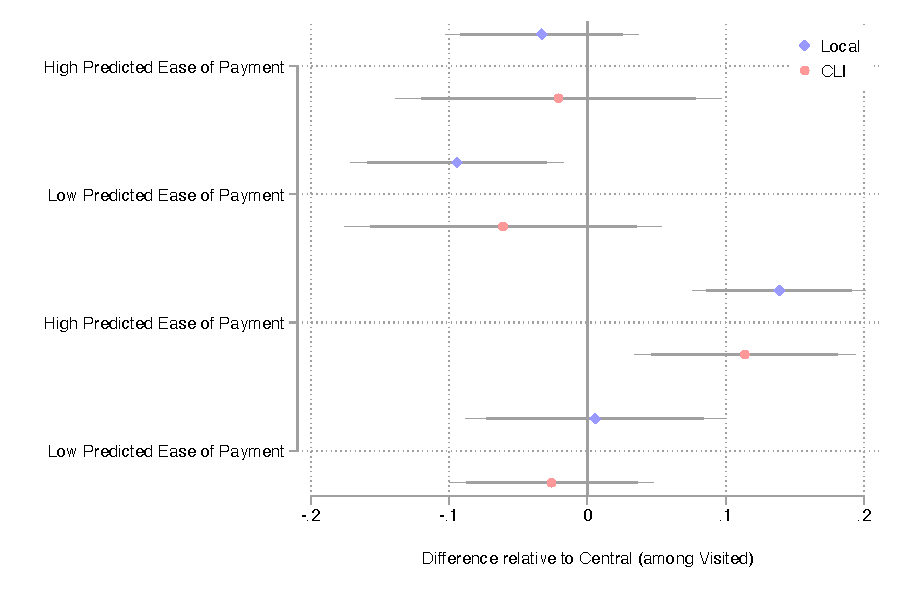
\includegraphics[scale=.7]{Output/chars_PEXHQ.pdf}\\
B: Predicted Ease of Payment and House Quality\\
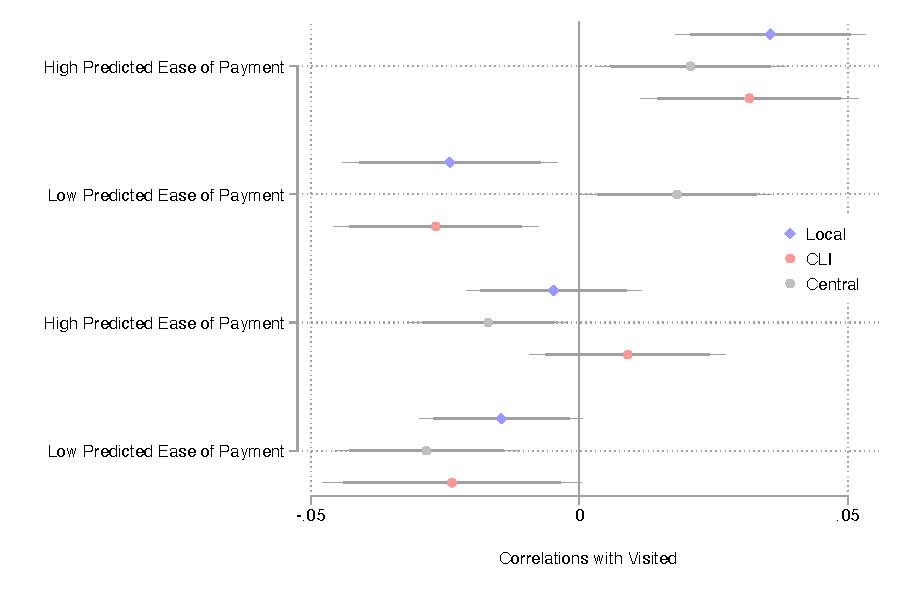
\includegraphics[scale=.7]{Output/chars_PEXHQ_bytmt.pdf}\\
\end{tabular}
}
\usebox{\tablebox}\\[1ex]
\parbox{6in}{\footnotesize \textit{Notes}: This figure reports correlations by treatment arm in the characteristics of properties visited by collectors after registration. It therefore supplements the analysis in Figure \ref{fig:main_targeting1}, which examines \textit{differences by treatment} in the characteristics of households that received tax visits after registration. Panel A shows correlations with visible and non-visible characteristics for indices described in Section \ref{targeting_discussion}.  Panel B shows correlations with tax visits in the four cells indicated (defined by interactions of high/low dummies for household house quality and predicted ease of payment). Correlations are estimated through separate regressions of characteristics on a treatment indicator among visited properties, controlling for the leave-one-out neighborhood mean of the outcome (Panel A) or the neighborhood mean of house quality and ease of payment (Panel B). We include time period, house type, and stratum fixed effects. We cluster standard errors at the neighborhood level. Households that paid at registration are dropped. This figure is discussed in Section \ref{targeting_discussion}.}
\end{figure}

%%%%%%%%%%%%%%%%%%%%%%%%%%%%%%%%%%%%%%%%%%%%%%%%%%%%%%%%%%%%%%%%%

\begin{figure}[H]
\centering{}\caption{Characteristics of Households Visited by Collectors After Registration Across Treatments --- No House Fixed Effects
\label{fig:main_targeting1_NoHouseFE}}
\centering
\centerfloat
\begin{tabular}{c}
A: Visible and Non-Visible Characteristics\\
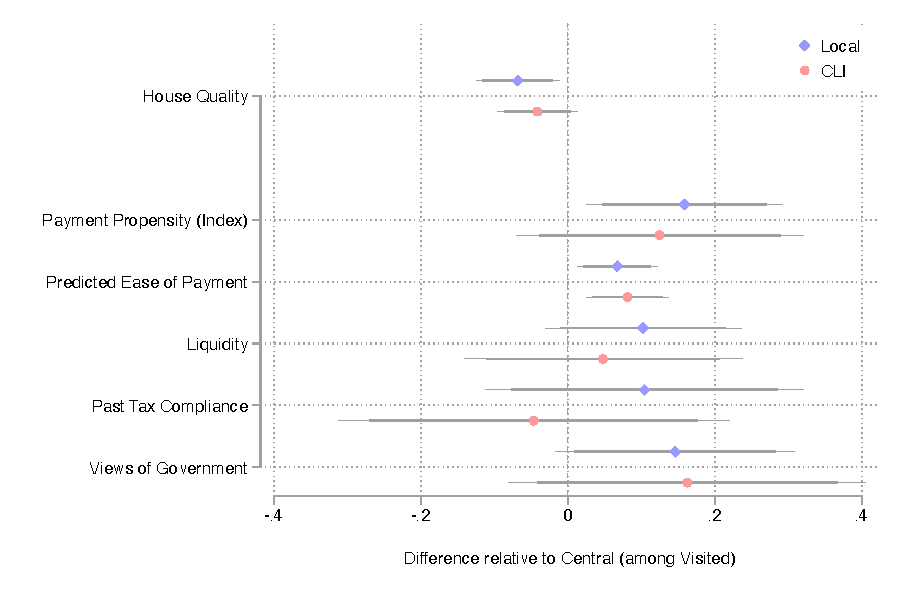
\includegraphics[scale=.7]{Output/chars_visited_nohouseFE.pdf}\\
B: Willingness to Pay and House Quality\\
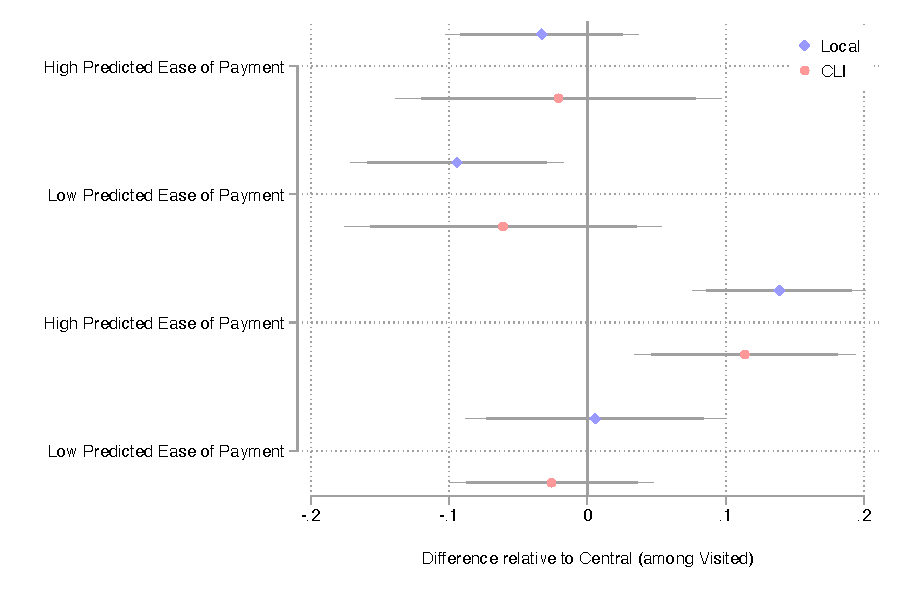
\includegraphics[scale=.7]{Output/chars_PEXHQ_nohouseFE.pdf}\\
\end{tabular}
\usebox{\tablebox}\\[1ex]
\parbox{6in}{\footnotesize \textit{Notes}: This figure reproduces the results from Figure \ref{fig:main_targeting1} but excludes house fixed effects as a robustness check. Specifically, it reports differences by treatment arm in the characteristics of properties visited by collectors after registration, showing differences in characteristics of visited properties in the Local and CLI arms relative to the Central arm. Panel A shows differences in visible and non-visible characteristics for indices described in Section \ref{targeting_discussion}. Panel B shows differences in the probability of receiving a visit in the four cells indicated (defined by interactions of high/low dummies for household house quality and predicted ease of payment). Differences are estimated through separate regressions of characteristics on a treatment indicator among visited properties, controlling for the leave-one-out neighborhood mean of the outcome (Panel A) or the neighborhood mean of house quality and ease of payment (Panel B). We include time period, house type, and stratum fixed effects. We cluster standard errors at the neighborhood level. Households that paid during registration are dropped. We discuss these results in Section \ref{targeting_discussion}.}
\end{figure}

%%%%%%%%%%%%%%%%%%%%%%%%%%%%%%%%%%%%%%%%%%%%%%%%%%%%%%%%%%%%%%%%%

\begin{figure}[H]
\centering{}\caption{Characteristics of Households Visited by Tax Collectors After Registration Across Treatments --- Omitting Neighborhood Mean Controls
\label{main_targeting_noControlMean_appendix}}
\centering
\centerfloat
\scalebox{0.9}{
\begin{tabular}{c}
A: Visible and Non-Visible Characteristics\\
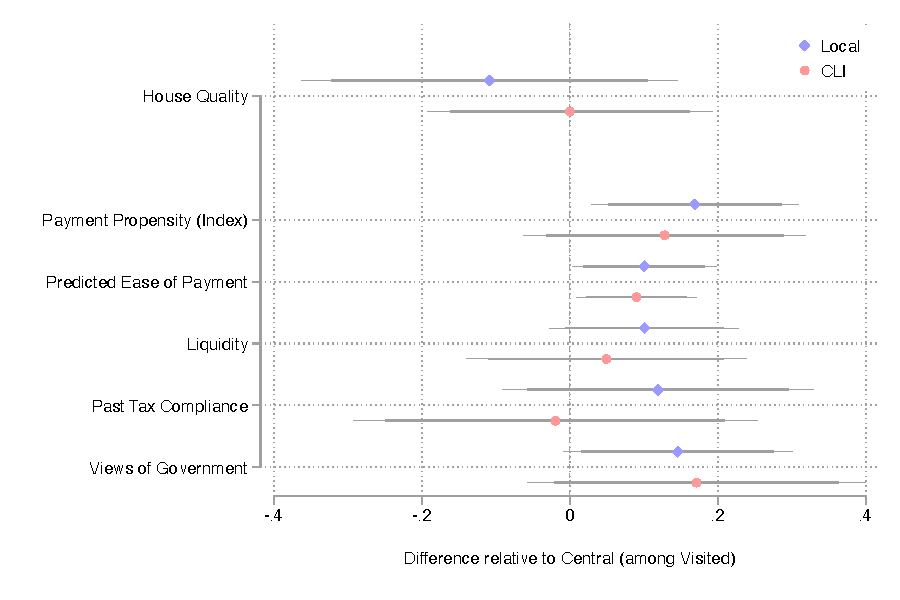
\includegraphics[scale=.7]{Output/chars_visited_nonbhdmean.pdf}\\
B: Willingness to Pay and House Quality\\
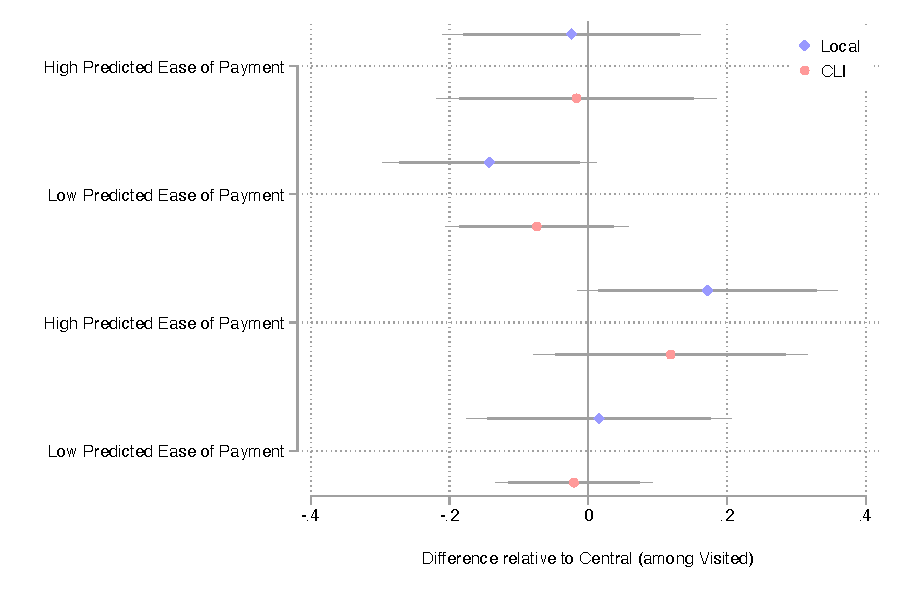
\includegraphics[scale=.7]{Output/chars_PEXHQ_nonbhdmean.pdf}\\
\end{tabular}
}
\usebox{\tablebox}\\[1ex]
\parbox{6in}{\footnotesize \textit{Notes}: This figure reproduces the results from Figure \ref{fig:main_targeting1} but omits the neighborhood mean controls as a robustness check. Specifically, it reports differences by treatment arm in the characteristics of properties visited by collectors after registration, showing differences in characteristics of visited properties in the Local and CLI arms relative to the Central arm. Panel A shows differences in visible and non-visible characteristics for indices described in Section \ref{targeting_discussion}. Panel B shows differences in the probability of receiving a visit in the four cells indicated (defined by interactions of high/low dummies for household house quality and predicted ease of payment). Differences are estimated through separate regressions of characteristics on a treatment indicator among visited properties, controlling for the leave-one-out neighborhood mean of the outcome (Panel A) or the neighborhood mean of house quality and ease of payment (Panel B). We include time period, house type, and stratum fixed effects. We cluster standard errors at the neighborhood level. Households that paid during registration are dropped. We discuss these results in Section \ref{targeting_discussion}.}
\end{figure}

%%%%%%%%%%%%%%%%%%%%%%%%%%%%%%%%%%%%%%%%%%%%%%%%%%%%%%%%%%%%%%%%%

\newgeometry{verbose, tmargin=0.8in, bmargin=1in, lmargin=1.2in, rmargin=1.2in}

%%%%%%%%%%%%%%%%%%%%%%%%%%%%%%%%%%%%%%%%%%%%%%%%%%%%%%%%%%%%%%%%%

\begin{figure}[H]
\centering{}\caption{Correlations between Tax Visits and Chief Connections
\label{main_targeting_chiefchar_appendix}}
\centering
\centerfloat
\begin{tabular}{c}
A: Local and CLI v. Central \\
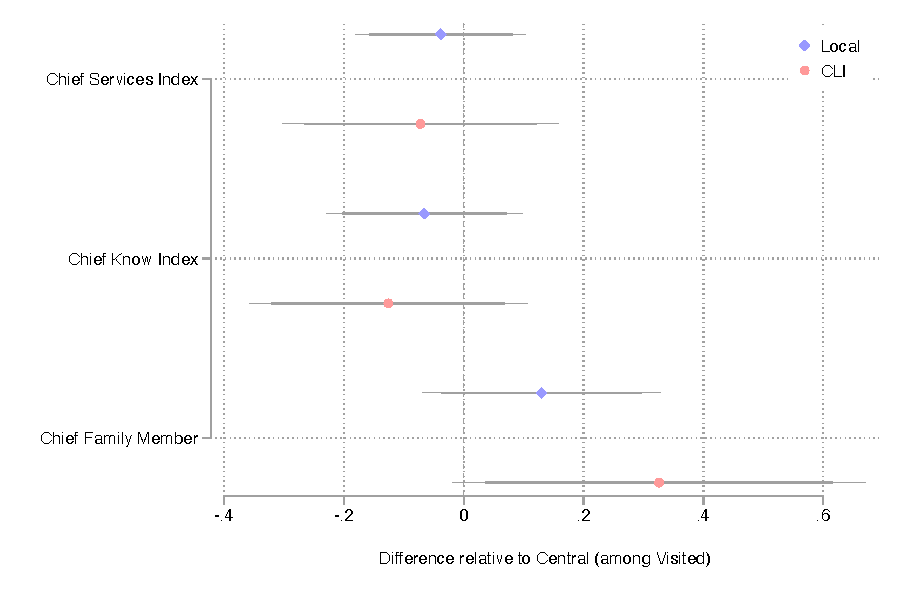
\includegraphics[scale=.55]{Output/chief_indices_CvL.pdf} \\
B: CLI v. Local \\
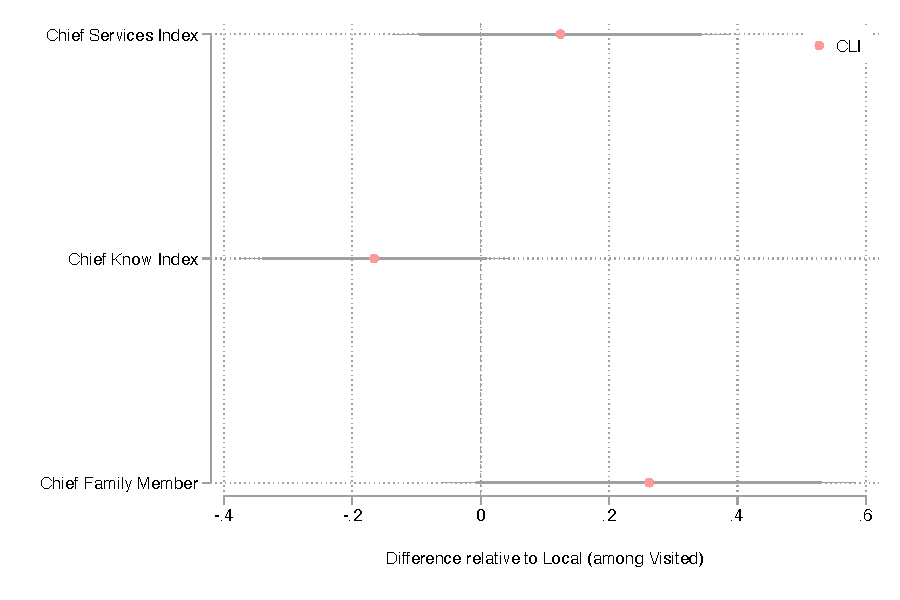
\includegraphics[scale=.55]{Output/chief_indices_LvCLI.pdf}\\
C: Correlations by Treatment\\
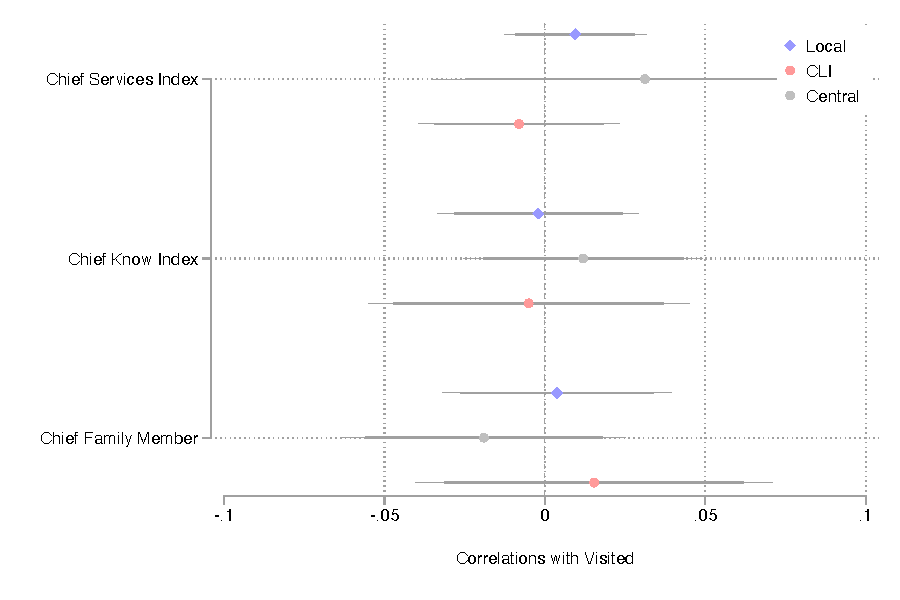
\includegraphics[scale=.55]{Output/chief_indices_bytmt.pdf}\\
\end{tabular}
\usebox{\tablebox}\\[1ex]
\parbox{6in}{\footnotesize \textit{Notes}: This figure reports differences and correlations by treatment arm in the probability of receiving tax visits after registration and households' connections to the chief. Panel A shows differences in terms of the indices described in Section \ref{targeting_discussion}, comparing Local and CLI to Central.  Panel B shows differences comparing CLI to Local. Panel C shows correlations with tax visits by treatment.  Differences are estimated through separate regressions of the connection variable on a treatment indicator, controlling for the leave-one-out neighborhood mean.  Correlations are estimated through separate regressions of an indicator for receiving a tax visit on a characteristic separately by treatment groups.   All regressions control for the leave-one-out neighborhood mean of the connection variable and include time period, house type, and stratum fixed effects and clustering standard errors at the neighborhood level.  Households that paid at registration are dropped. We discuss these results in Section \ref{targeting_discussion}.}
\end{figure}

%%%%%%%%%%%%%%%%%%%%%%%%%%%%%%%%%%%%%%%%%%%%%%%%%%%%%%%%%%%%%%%%%

\clearpage

%%%%%%%%%%%%%%%%%%%%%%%%%%%%%%%%%%%%%%%%%%%%%%%%%%%%%%%%%%%%%%%%%

\newgeometry{verbose, tmargin=1in, bmargin=1in, lmargin=1.2in, rmargin=1.2in}

%%%%%%%%%%%%%%%%%%%%%%%%%%%%%%%%%%%%%%%%%%%%%%%%%%%%%%%%%%%%%%%%%

\begin{landscape}

%%%%%%%%%%%%%%%%%%%%%%%%%%%%%%%%%%%%%%%%%%%%%%%%%%%%%%%%%%%%%%%%%

\begin{table}[H]
\vspace*{-1cm}
\textbf{\caption{\label{ethnicity} Local v. Central: Tax Visits and Compliance by Coethnicity}}
\centering
\begin{lrbox}{\tablebox}
\resizebox{18cm}{!}{
{
\def\sym#1{\ifmmode^{#1}\else\(^{#1}\)\fi}
\begin{tabular}{l*{6}{c}}
\hline\hline
                &\multicolumn{1}{c}{Tribe}&\multicolumn{1}{c}{Subtribe}&\multicolumn{1}{c}{Lang. Maj.}&\multicolumn{1}{c}{Tribe}&\multicolumn{1}{c}{Subtribe}&\multicolumn{1}{c}{Lang. Maj.}\\
                &\multicolumn{1}{c}{(1)}         &\multicolumn{1}{c}{(2)}         &\multicolumn{1}{c}{(3)}         &\multicolumn{1}{c}{(4)}         &\multicolumn{1}{c}{(5)}         &\multicolumn{1}{c}{(6)}         \\
\hline
Local           &   -0.002         &    0.063         &   -0.016         &    0.050\sym{***}&    0.026         &    0.049\sym{**} \\
                &  (0.031)         &  (0.044)         &  (0.039)         &  (0.011)         &  (0.019)         &  (0.017)         \\
hetXt\_l         &    0.007         &   -0.117\sym{**} &    0.020         &   -0.015         &   -0.035         &   -0.003         \\
                &  (0.040)         &  (0.058)         &  (0.045)         &  (0.016)         &  (0.044)         &  (0.019)         \\
het             &   -0.010         &    0.143\sym{**} &   -0.004         &    0.011         &    0.051         &   -0.009         \\
                &  (0.035)         &  (0.054)         &  (0.035)         &  (0.013)         &  (0.041)         &  (0.012)         \\
Time FE         &      Yes         &      Yes         &      Yes         &      Yes         &      Yes         &      Yes         \\
House FE        &      Yes         &      Yes         &      Yes         &      Yes         &      Yes         &      Yes         \\
Stratum FE      &      Yes         &      Yes         &      Yes         &      Yes         &      Yes         &      Yes         \\
\hline
Observations    &    13628         &     6457         &    13628         &    13752         &     6491         &    13752         \\
Mean            &     .438         &     .297         &     .432         &     .072         &     .052         &     .074         \\
Polygons        &      210         &      114         &      210         &      210         &      114         &      210         \\
\hline\hline
\end{tabular}
}

}
\end{lrbox}
\usebox{\tablebox}\\[1ex]
\parbox{7in}{\footnotesize \textit{Notes}: This table reports estimates from a version of Equation \ref{equation_cvl}, comparing tax visits and compliance in Local and Central (the excluded category) by whether the collector and property owner are coethnics along a specific dimension. The outcome in Columns 1--3 is whether households reported any tax visits after registration. The outcome in Columns 4--6 is compliance according to administrative data. Match corresponds to an indicator for the chief's or at least one state collector's coethnicity characteristic matching that of the property owner for the characteristics at the top of each column. Columns 1 and 5 show estimates for including an interaction with an indicator for a collector's and property owner's tribe matching, Columns 2 and 6 for subtribe, Columns 3 and 7 for both being members of the language majority, and Columns 4 and 8 for families originating from the same territory. All regressions include fixed effects for time periods described in Section \ref{estimation}, house type, and randomization strata. We cluster standard errors at the neighborhood level. These results are discussed in Section \ref{targeting_discussion}.}
\end{table}

%%%%%%%%%%%%%%%%%%%%%%%%%%%%%%%%%%%%%%%%%%%%%%%%%%%%%%%%%%%%%%%%%

\end{landscape}

%%%%%%%%%%%%%%%%%%%%%%%%%%%%%%%%%%%%%%%%%%%%%%%%%%%%%%%%%%%%%%%%%

\begin{table}[H]
%\vspace*{-1cm}
\textbf{\caption{\label{Table_CvL_Distribution_Incidence_NoHouseFE} Local v. Central: The Distribution of the Tax Burden --- No House Fixed Effects}}
\centering
\begin{lrbox}{\tablebox}
\resizebox{15cm}{!}{
{
\def\sym#1{\ifmmode^{#1}\else\(^{#1}\)\fi}
\begin{tabular}{l*{5}{c}}
\hline\hline
                &\multicolumn{1}{c}{Paid - Periph}&\multicolumn{1}{c}{Paid - MM}&\multicolumn{1}{c}{HQ - Visited}&\multicolumn{1}{c}{HQ - Paid}&\multicolumn{1}{c}{Income - Visited}\\
                &\multicolumn{1}{c}{(1)}         &\multicolumn{1}{c}{(2)}         &\multicolumn{1}{c}{(3)}         &\multicolumn{1}{c}{(4)}         &\multicolumn{1}{c}{(5)}         \\
\hline
Local           &    0.037\sym{***}&    0.002         &   -0.142\sym{**} &   -0.003         &   -0.079         \\
                &  (0.008)         &  (0.013)         &  (0.056)         &  (0.038)         &  (0.161)         \\
Month FE        &      Yes         &      Yes         &      Yes         &      Yes         &      Yes         \\
Stratum FE      &      Yes         &      Yes         &      Yes         &      Yes         &      Yes         \\
\hline
Observations    &    24105         &     3265         &     1296         &      224         &      224         \\
Clusters        &      206         &      147         &      156         &      120         &      120         \\
Mean            &     .064         &     .063         &     .099         &     .007         &     .118         \\
\hline\hline
\end{tabular}
}

}
\end{lrbox}
\usebox{\tablebox}\\[1ex]
\parbox{6in}{\footnotesize \textit{Notes}: This table re-estimates the results reported in Table \ref{Table_CvL_Distribution_Incidence} while excluding house fixed effects. Specifically, it reports estimates from a version of Equation \ref{equation_cvl}, comparing property tax compliance in Local and Central (the excluded category). We include fixed effects for randomization strata and time periods, as described in Section \ref{estimation}, and we cluster standard errors at the neighborhood level. Columns 1 and 2 report estimates of the impact of local collection on compliance for low- and high-band households, respectively. Column 3 reports differences in an index of house quality conditional on the property paying the tax.  Column 4 reports differences in monthly household income of properties, averaged across baseline and endline values, in Congolese Francs, conditional on paying the tax.  Column 5 reports differences in an index of liquidity measures drawn from baseline (excepting income, which is also included, and uses information from endline) among payers. Columns 3--5 control for the leave-one-out neighborhood mean of the outcome. We discuss the interpretation of these results in Section \ref{incidence_discussion}.}
\end{table}

%%%%%%%%%%%%%%%%%%%%%%%%%%%%%%%%%%%%%%%%%%%%%%%%%%%%%%%%%%%%%%%%%

\begin{table}[H]
\textbf{\caption{\label{Table_CvLvCLI_Distribution_Incidence} Local and CLI v. Central: Incidence by Complier Characteristics --- No Neighborhood Mean Controls}}
\centering
\begin{lrbox}{\tablebox}
\resizebox{16cm}{!}{
{
\def\sym#1{\ifmmode^{#1}\else\(^{#1}\)\fi}
\begin{tabular}{l*{6}{c}}
\hline\hline
                &\multicolumn{1}{c}{HQ - Paid}&\multicolumn{1}{c}{Income - Paid}&\multicolumn{1}{c}{Liquidity - Paid}&\multicolumn{1}{c}{HQ - Paid}&\multicolumn{1}{c}{Income - Paid}&\multicolumn{1}{c}{Liquidity - Paid}\\
                &\multicolumn{1}{c}{(1)}         &\multicolumn{1}{c}{(2)}         &\multicolumn{1}{c}{(3)}         &\multicolumn{1}{c}{(4)}         &\multicolumn{1}{c}{(5)}         &\multicolumn{1}{c}{(6)}         \\
\hline
Local           &   -0.216         &    0.002         &   -0.053         &                  &                  &                  \\
                &  (0.156)         &  (0.041)         &  (0.174)         &                  &                  &                  \\
CLI             &                  &                  &                  &    0.133         &    0.015         &    0.183         \\
                &                  &                  &                  &  (0.127)         &  (0.053)         &  (0.211)         \\
Month FE        &      Yes         &      Yes         &      Yes         &      Yes         &      Yes         &      Yes         \\
House FE        &      Yes         &      Yes         &      Yes         &      Yes         &      Yes         &      Yes         \\
Stratum FE      &      Yes         &      Yes         &      Yes         &      Yes         &      Yes         &      Yes         \\
\hline
Observations    &     1310         &      228         &      228         &      832         &      141         &      141         \\
Clusters        &      157         &      121         &      121         &      118         &       87         &       87         \\
Mean            &     .099         &     .007         &     .118         &     .096         &      .02         &     .193         \\
\hline\hline
\end{tabular}
}

}
\end{lrbox}
\usebox{\tablebox}\\[1ex]
\parbox{6in}{\footnotesize \textit{Notes}: This table re-estimates the results reported in Columns 3--5 of Table \ref{Table_CvL_Distribution_Incidence} while excluding controls for the neighborhood mean. Columns 1--3 examine the distribution of the noted characteristics among taxpayers in a comparison of Local v. Central, while Columns 4--6 compare CLI v. Central. Column 1 and 4 report differences in an index of house quality conditional on the property paying the tax.  Columns 2 and 5 report differences in monthly household income of properties, averaged across baseline and endline values, in Congolese Francs, conditional on paying the tax. Columns 3 and 6 report differences in an index of liquidity measures drawn from baseline (except income, which is also included, and uses information from endline) among payers. We include fixed effects for house type, randomization strata, and time periods, as described in Section \ref{estimation}, and we cluster standard errors at the neighborhood level. We discuss the interpretation of these results in Section \ref{incidence_discussion}.}
\end{table}

%%%%%%%%%%%%%%%%%%%%%%%%%%%%%%%%%%%%%%%%%%%%%%%%%%%%%%%%%%%%%%%%%

\begin{table}[H]
\vspace{-1.2cm}
\textbf{\caption{Local v. Central: The Distribution of the Tax Burden --- Property Value Band Interactions \label{PaperTable_CvL_Incidence_HouseTypeInteraction}}}
\centering
\centerfloat
\begin{lrbox}{\tablebox}
\scalebox{.9}{
{
\def\sym#1{\ifmmode^{#1}\else\(^{#1}\)\fi}
\begin{tabular}{l*{2}{c}}
\hline\hline
                &\multicolumn{1}{c}{Compliance}&\multicolumn{1}{c}{Revenues}\\
                &\multicolumn{1}{c}{(1)}         &\multicolumn{1}{c}{(2)}         \\
\hline
Local           &    0.037\sym{***}&   77.607\sym{***}\\
                &  (0.008)         & (17.844)         \\
Local X High-Value Band&   -0.029\sym{**} &  -73.065         \\
                &  (0.013)         & (96.963)         \\
High-Value Band &   -0.014         &  398.778\sym{***}\\
                &  (0.009)         & (69.284)         \\
Month FE        &      Yes         &      Yes         \\
Stratum FE      &      Yes         &      Yes         \\
\hline
Observations    &    27764         &    27764         \\
Clusters        &      213         &      213         \\
Mean            &     .064         &  133.152         \\
\hline\hline
\end{tabular}
}

}
\end{lrbox}
\usebox{\tablebox}\\[1ex]
\parbox{6.3in}{\footnotesize{\textit{Notes}: This figure reports estimates from a version of Equation \ref{equation_cvl}, showing differences in tax payment in the Local arm relative to the Central arm by heterogeneity in property value band assessed at registration --- an interaction version of the specification in Table \ref{Table_CvL_Distribution_Incidence}, Columns 1--2. We include time period and stratum fixed effects and cluster standard errors at the neighborhood level. We discuss the interpretation of these results in Section \ref{incidence_discussion}.}}
\end{table}

%%%%%%%%%%%%%%%%%%%%%%%%%%%%%%%%%%%%%%%%%%%%%%%%%%%%%%%%%%%%%%%%%

\begin{table}[H]
\vspace{-1.2cm}
\textbf{\caption{Local v. Central: The Distribution of the Tax Burden --- Complier Characteristics Interactions \label{PaperTable_CvL_Incidence_Cols3to5Interactions}}}
\centering
\centerfloat
{
\def\sym#1{\ifmmode^{#1}\else\(^{#1}\)\fi}
\begin{tabular}{l*{3}{c}}
\hline\hline
                &\multicolumn{1}{c}{HQ Compliance}&\multicolumn{1}{c}{Inc Compliance}&\multicolumn{1}{c}{Liq Compliance}\\
                &\multicolumn{1}{c}{(1)}         &\multicolumn{1}{c}{(2)}         &\multicolumn{1}{c}{(3)}         \\
\hline
Local           &    0.053\sym{***}&    0.017         &    0.019         \\
                &  (0.009)         &  (0.031)         &  (0.031)         \\
Local X Above Median&   -0.004         &    0.013         &    0.011         \\
                &  (0.011)         &  (0.036)         &  (0.036)         \\
Above Median    &    0.034\sym{***}&    0.022         &    0.023         \\
                &  (0.006)         &  (0.025)         &  (0.025)         \\
Month FE        &      Yes         &      Yes         &      Yes         \\
House FE        &      Yes         &      Yes         &      Yes         \\
Stratum FE      &      Yes         &      Yes         &      Yes         \\
\hline
Observations    &    17519         &     2236         &     2238         \\
Clusters        &      174         &      212         &      212         \\
Mean            &     .045         &      .06         &      .06         \\
\hline\hline
\end{tabular}
}

\\
{
\def\sym#1{\ifmmode^{#1}\else\(^{#1}\)\fi}
\begin{tabular}{l*{3}{c}}
\hline\hline
                &\multicolumn{1}{c}{HQ Revenues}&\multicolumn{1}{c}{Inc Revenues}&\multicolumn{1}{c}{Liq Revenues}\\
                &\multicolumn{1}{c}{(1)}         &\multicolumn{1}{c}{(2)}         &\multicolumn{1}{c}{(3)}         \\
\hline
Local           &  121.651\sym{***}&   90.690         &  106.947         \\
                & (23.516)         & (75.542)         & (81.553)         \\
t\_lXhetmargin   &  -24.687         &  -38.534         &  -57.080         \\
                & (28.456)         & (87.068)         & (92.835)         \\
hetmargin       &   87.670\sym{***}&   92.759         &  102.466\sym{*}  \\
                & (20.038)         & (57.610)         & (56.979)         \\
Month FE        &      Yes         &      Yes         &      Yes         \\
House FE        &      Yes         &      Yes         &      Yes         \\
Stratum FE      &      Yes         &      Yes         &      Yes         \\
\hline
Observations    &    17519         &     2236         &     2238         \\
Clusters        &      174         &      212         &      212         \\
Mean            &   96.541         &  115.385         &  115.385         \\
\hline\hline
\end{tabular}
}

\usebox{\tablebox}\\[1ex]
\parbox{6.3in}{\footnotesize{\textit{Notes}: This figure reports estimates from a version of Equation \ref{equation_cvl}, showing differences in tax payment in the Local arm relative to the Central arm by heterogeneity in the incidence measures described in Table \ref{Table_CvL_Distribution_Incidence}, Columns 3--5: house quality, average monthly income, and an index of liquidity, interacting an indicator for the Local arm with indicators for having above-median values for each measure. We include time period, house type, and stratum fixed effects and cluster standard errors at the neighborhood level. We also include controls for the the leave-one-out neighborhood means of the relevant heterogeneity measure. We discuss the interpretation of these results in Section \ref{incidence_discussion}.}}
\end{table}

%%%%%%%%%%%%%%%%%%%%%%%%%%%%%%%%%%%%%%%%%%%%%%%%%%%%%%%%%%%%%%%%%

\begin{figure}[H]
\centering{}\caption{House Quality, Income, and Liquidity Distributions Among Visited and Paying Households By Treatment
\label{fig:distribution_all}}
\centerfloat
\begin{tabular}{cc}
A: House quality - Visited owners & B: House quality - Taxpayers  \\
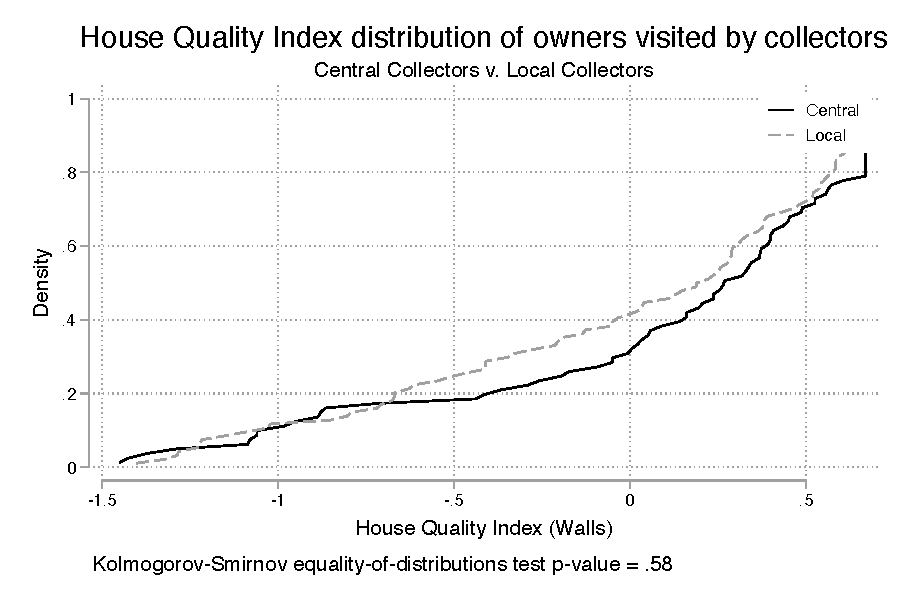
\includegraphics[scale=.55]{Output/dist_housequal_visited.pdf} & 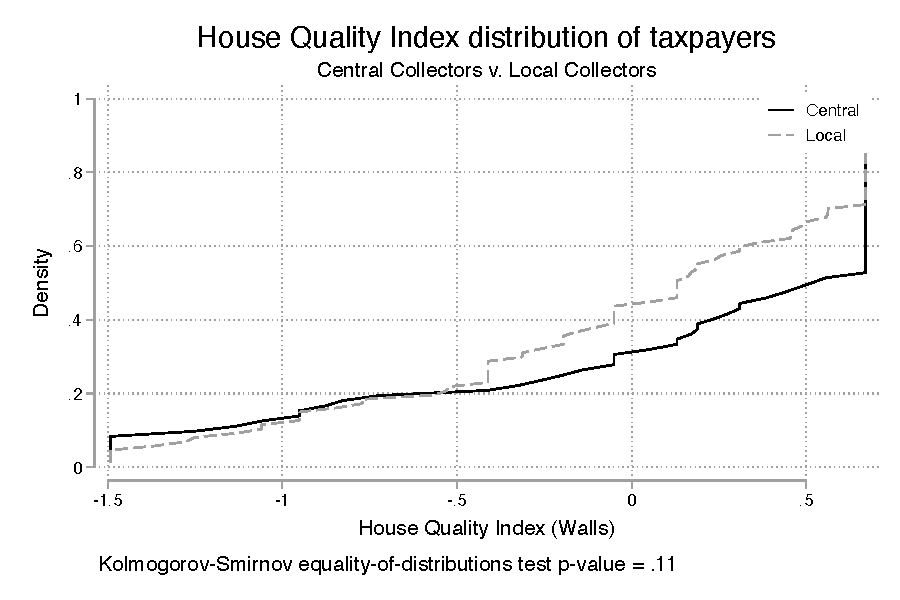
\includegraphics[scale=.55]{Output/dist_housequal_taxpayers.pdf}\\
C: Income - Visited owners & D: Income - Taxpayers  \\
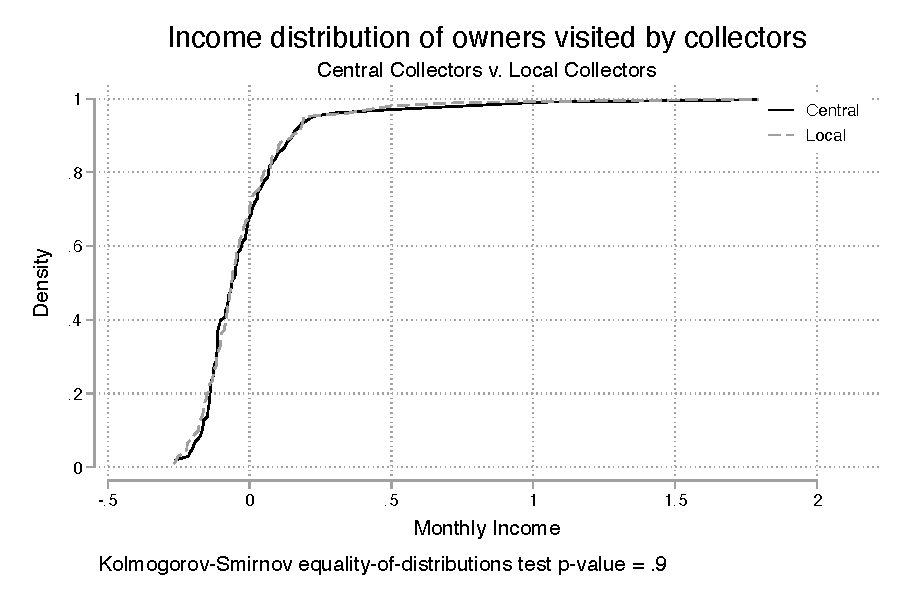
\includegraphics[scale=.55]{Output/dist_inc_visited.pdf} & 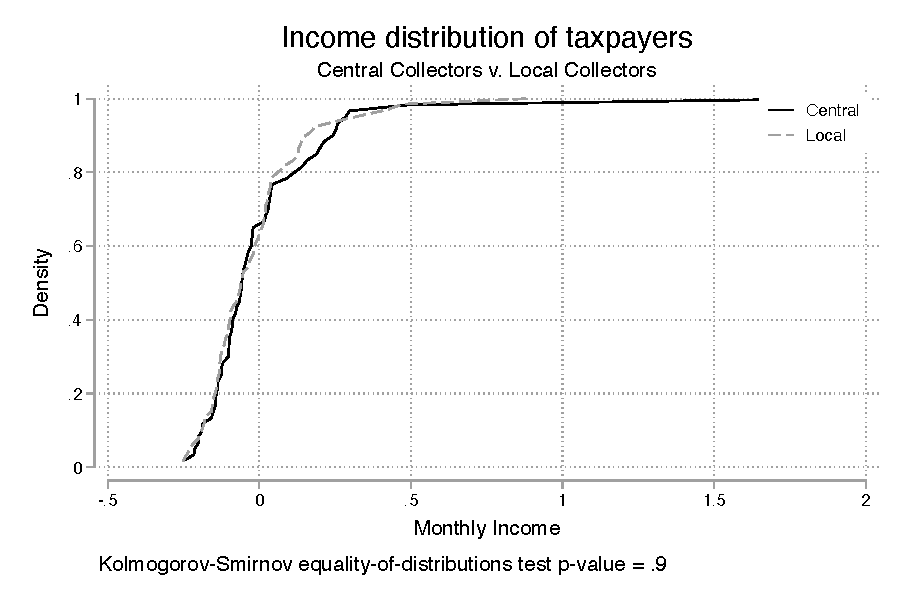
\includegraphics[scale=.55]{Output/dist_inc_taxpayers.pdf}\\
E: Liquidity - Visited owners & F: Liquidity - Taxpayers  \\
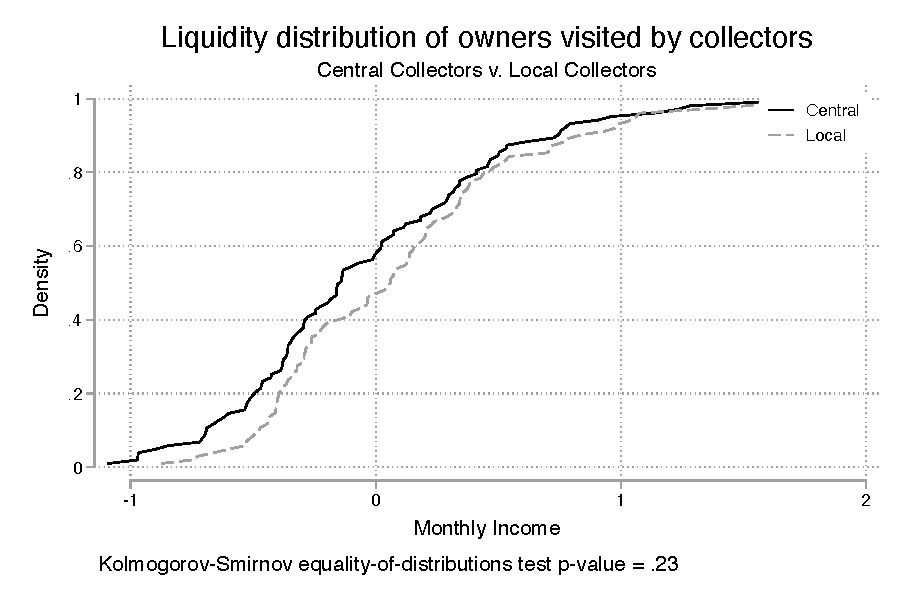
\includegraphics[scale=.55]{Output/dist_liq_visited.pdf} & 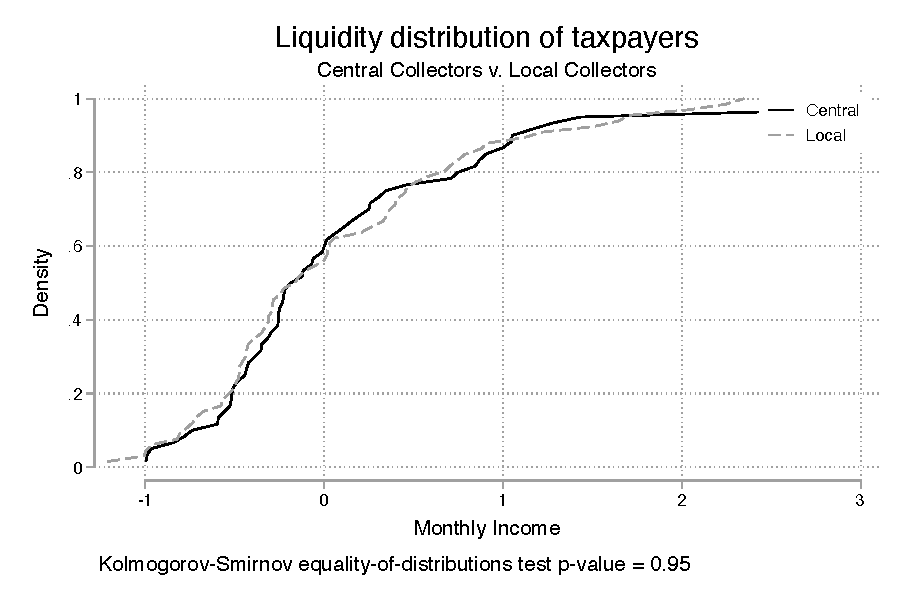
\includegraphics[scale=.55]{Output/dist_liq_taxpayers.pdf}\\
\end{tabular}
\usebox{\tablebox}\\[1ex]
\parbox{6in}{\footnotesize \textit{Notes}: This figure shows cumulative distribution functions of house quality and income by treatment and separately among households that received tax visits after registration (Panels A, C, and E) and that paid the tax (Panels B, D, and F). In Panel B, the taxpayer distribution has considerable mass at the maximum value of the house quality index in Central, making the CDF somewhat difficult to read. Kolmogorov-Smirnov equality of distributions test $p$-values are reported at the bottom. We discuss these results in Section \ref{incidence_discussion}.}
\end{figure}

%%%%%%%%%%%%%%%%%%%%%%%%%%%%%%%%%%%%%%%%%%%%%%%%%%%%%%%%%%%%%%%%%

\clearpage

%%%%%%%%%%%%%%%%%%%%%%%%%%%%%%%%%%%%%%%%%%%%%%%%%%%%%%%%%%%%%%%%%

\clearpage

%%%%%%%%%%%%%%%%%%%%%%%%%%%%%%%%%%%%%%%%%%%%%%%%%%%%%%%%%%%%%%%%%

\subsection{Additional Exhibits for Paper Section 9 --- Policy Implications}

%%%%%%%%%%%%%%%%%%%%%%%%%%%%%%%%%%%%%%%%%%%%%%%%%%%%%%%%%%%%%%%%%

\begin{figure}[H]
\centering{}\caption{Local v. Central + Local Info: Differences in Targeting of Tax Visits by Household Characteristics
\label{main_targeting_appendix_LvCLI}}
\centering
\centerfloat
\begin{tabular}{c}
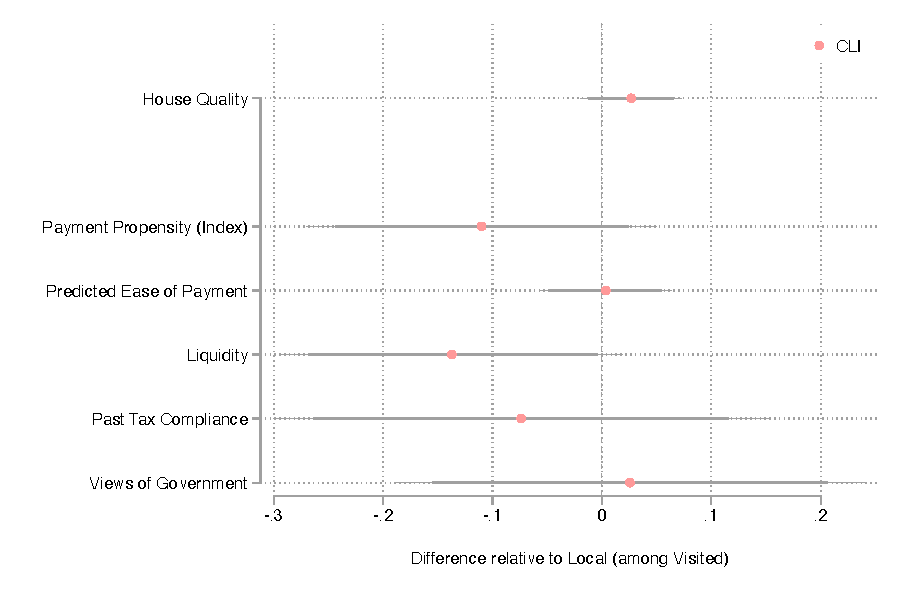
\includegraphics[scale=.7]{Output/chars_visited_LvCLI.pdf}\\
\end{tabular}
\usebox{\tablebox}\\[1ex]
\parbox{6in}{\footnotesize \textit{Notes}: This figure reports correlations by treatment arm in the characteristics of properties visited by collectors after registration. The figure shows differences in visible and non-visible characteristics for indices described in Section \ref{targeting_discussion}. Correlations are estimated through separate regressions of an indicator for receiving a tax visit on a characteristic separately by treatment groups, controlling for the leave-one-out neighborhood mean of the outcome, including time period, house type, and stratum fixed effects and clustering standard errors at the neighborhood level.  Households that paid at registration are dropped. We discuss these results in Section \ref{codifiability}.}
\end{figure}

%%%%%%%%%%%%%%%%%%%%%%%%%%%%%%%%%%%%%%%%%%%%%%%%%%%%%%%%%%%%%%%%%

\clearpage
\pagebreak

%%%%%%%%%%%%%%%%%%%%%%%%%%%%%%%%%%%%%%%%%%%%%%%%%%%%%%%%%%%%%%%%%

\begin{landscape}

%%%%%%%%%%%%%%%%%%%%%%%%%%%%%%%%%%%%%%%%%%%%%%%%%%%%%%%%%%%%%%%%%

\begin{table}[H]
\vspace*{-1cm}
\textbf{\caption{\label{welfare1} Local v. Central: Impacts on Household Well-Being}}
\centering
\tiny{{
\def\sym#1{\ifmmode^{#1}\else\(^{#1}\)\fi}
\begin{tabular}{l*{7}{c}}
\hline\hline
                &\multicolumn{1}{c}{Monthly Income}&\multicolumn{1}{c}{Weekly Transport}&\multicolumn{1}{c}{Bed Hungry Last month Yes/No}&\multicolumn{1}{c}{Bed Hungry Last month Nb of days}&\multicolumn{1}{c}{3000 CF in cash today}&\multicolumn{1}{c}{lacks 3000 CF in cash this month}&\multicolumn{1}{c}{lacks 3000 CF in cash this month NB of days}\\
                &\multicolumn{1}{c}{(1)}         &\multicolumn{1}{c}{(2)}         &\multicolumn{1}{c}{(3)}         &\multicolumn{1}{c}{(4)}         &\multicolumn{1}{c}{(5)}         &\multicolumn{1}{c}{(6)}         &\multicolumn{1}{c}{(7)}         \\
\hline
Local           &-2300.525         &  -37.852         &   -0.015         &   -0.017         &   -0.014         &   -0.003         &    0.105         \\
                &(7800.918)         &(438.961)         &  (0.023)         &  (0.077)         &  (0.023)         &  (0.027)         &  (0.176)         \\
House FE        &      Yes         &      Yes         &      Yes         &      Yes         &      Yes         &      Yes         &      Yes         \\
Stratum FE      &      Yes         &      Yes         &      Yes         &      Yes         &      Yes         &      Yes         &      Yes         \\
\hline
Observations    &     2277         &     2329         &     2330         &     2330         &     2330         &     2330         &     2330         \\
Mean            &144788.859         & 4455.783         &     .516         &     .993         &     .675         &     .652         &     1.29         \\
\hline\hline
\end{tabular}
}
}
\tiny{{
\def\sym#1{\ifmmode^{#1}\else\(^{#1}\)\fi}
\begin{tabular}{l*{7}{c}}
\hline\hline
                &\multicolumn{1}{c}{Monthly Income}&\multicolumn{1}{c}{Weekly Transport}&\multicolumn{1}{c}{Bed Hungry Last month Yes/No}&\multicolumn{1}{c}{Bed Hungry Last month Nb of days}&\multicolumn{1}{c}{3000 CF in cash today}&\multicolumn{1}{c}{lacks 3000 CF in cash this month}&\multicolumn{1}{c}{lacks 3000 CF in cash this month NB of days}\\
                &\multicolumn{1}{c}{(1)}         &\multicolumn{1}{c}{(2)}         &\multicolumn{1}{c}{(3)}         &\multicolumn{1}{c}{(4)}         &\multicolumn{1}{c}{(5)}         &\multicolumn{1}{c}{(6)}         &\multicolumn{1}{c}{(7)}         \\
\hline
taxes\_paid      &-1.34e+05         &-2574.310         &   -1.054         &   -1.181         &   -0.942         &   -0.180         &    7.147         \\
                &(4.86e+05)         &(30047.563)         &  (1.954)         &  (5.270)         &  (1.802)         &  (1.827)         & (12.946)         \\
House FE        &      Yes         &      Yes         &      Yes         &      Yes         &      Yes         &      Yes         &      Yes         \\
Stratum FE      &      Yes         &      Yes         &      Yes         &      Yes         &      Yes         &      Yes         &      Yes         \\
\hline
Observations    &     2277         &     2329         &     2330         &     2330         &     2330         &     2330         &     2330         \\
Mean            &144788.859         & 4455.783         &     .516         &     .993         &     .675         &     .652         &     1.29         \\
\hline\hline
\end{tabular}
}
}
\tiny{{
\def\sym#1{\ifmmode^{#1}\else\(^{#1}\)\fi}
\begin{tabular}{l*{7}{c}}
\hline\hline
                &\multicolumn{1}{c}{Monthly Income}&\multicolumn{1}{c}{Weekly Transport}&\multicolumn{1}{c}{Bed Hungry Last month Yes/No}&\multicolumn{1}{c}{Bed Hungry Last month Nb of days}&\multicolumn{1}{c}{3000 CF in cash today}&\multicolumn{1}{c}{lacks 3000 CF in cash this month}&\multicolumn{1}{c}{lacks 3000 CF in cash this month NB of days}\\
                &\multicolumn{1}{c}{(1)}         &\multicolumn{1}{c}{(2)}         &\multicolumn{1}{c}{(3)}         &\multicolumn{1}{c}{(4)}         &\multicolumn{1}{c}{(5)}         &\multicolumn{1}{c}{(6)}         &\multicolumn{1}{c}{(7)}         \\
\hline
taxbribe        &33221.221         &-1.49e+04         &   -0.366         &    0.770         &   -0.079         &   -0.115         &    3.098         \\
                &(1.90e+05)         &(19209.285)         &  (0.603)         &  (1.615)         &  (0.529)         &  (0.634)         &  (3.169)         \\
House FE        &      Yes         &      Yes         &      Yes         &      Yes         &      Yes         &      Yes         &      Yes         \\
Stratum FE      &      Yes         &      Yes         &      Yes         &      Yes         &      Yes         &      Yes         &      Yes         \\
\hline
Observations    &     1260         &     1287         &     1287         &     1287         &     1287         &     1287         &     1287         \\
Mean            &150899.013         & 5173.794         &     .482         &     .863         &      .67         &      .63         &      1.1         \\
\hline\hline
\end{tabular}
}
}
\usebox{\tablebox}\\[1ex]
\parbox{6in}{\footnotesize \textit{Notes}: This table reports estimates from a version of Equation \ref{equation_cvl}, endline measures of well-being in Local and Central (the excluded category). We include fixed effects for house type and randomization strata and cluster standard errors at the neighborhood level. Columns 1 and 2 report differences in monthly household income and weekly transport (a measure of spending).  Columns 3 and 4 report differences in whether the household went to bed hungry at least one day in the last month and how many days, respectively. Columns 5, 6, and 7 report differences in whether the household lacked 3,000 Congolese Francs to be able to make a payment at the date of survey, sometime in the last month, and how many times in the last month, respectively.  Panel A reports the reduced form results of a regression of outcomes on an indicator for the Local treatment.  Panel B regresses outcomes on an indicator for tax payment instrumented by an indicator for the Local treatment.  Panel C regresses outcomes on an indicator for paying a tax or bribe with an indicator for the Local treatment. We discuss these results in Section \ref{policy}.}
\end{table}

%%%%%%%%%%%%%%%%%%%%%%%%%%%%%%%%%%%%%%%%%%%%%%%%%%%%%%%%%%%%%%%%%

\end{landscape}

%%%%%%%%%%%%%%%%%%%%%%%%%%%%%%%%%%%%%%%%%%%%%%%%%%%%%%%%%%%%%%%%%

\clearpage

%%%%%%%%%%%%%%%%%%%%%%%%%%%%%%%%%%%%%%%%%%%%%%%%%%%%%%%%%%%%%%%%%

\begin{landscape}

%%%%%%%%%%%%%%%%%%%%%%%%%%%%%%%%%%%%%%%%%%%%%%%%%%%%%%%%%%%%%%%%%

\begin{table}[ht]
\textbf{\caption{\label{views_taxed_int} Local v. Central: Views of Government and Chiefs by Tax and Bribe Payment}}
\centering
\tiny{{
\def\sym#1{\ifmmode^{#1}\else\(^{#1}\)\fi}
\begin{tabular}{l*{8}{c}}
\hline\hline
                &\multicolumn{1}{c}{Views of govt (index)}&\multicolumn{1}{c}{Trust in govt}&\multicolumn{1}{c}{Resp. of govt.}&\multicolumn{1}{c}{Perf. of govt.}&\multicolumn{1}{c}{Views of chief (index)}&\multicolumn{1}{c}{Trust in chief}&\multicolumn{1}{c}{Resp. of chief.}&\multicolumn{1}{c}{Perf. of chief.}\\
                &\multicolumn{1}{c}{(1)}         &\multicolumn{1}{c}{(2)}         &\multicolumn{1}{c}{(3)}         &\multicolumn{1}{c}{(4)}         &\multicolumn{1}{c}{(5)}         &\multicolumn{1}{c}{(6)}         &\multicolumn{1}{c}{(7)}         &\multicolumn{1}{c}{(8)}         \\
\hline
Local           &    0.036         &    0.153\sym{**} &   -0.057         &   -0.036         &    0.070         &    0.057         &   -0.039         &    0.085         \\
                &  (0.052)         &  (0.060)         &  (0.046)         &  (0.055)         &  (0.053)         &  (0.056)         &  (0.059)         &  (0.063)         \\
Local X Taxes Paid&   -0.090         &   -0.288\sym{*}  &    0.148         &   -0.184         &   -0.155         &   -0.143         &   -0.326\sym{**} &    0.057         \\
                &  (0.118)         &  (0.151)         &  (0.137)         &  (0.138)         &  (0.132)         &  (0.136)         &  (0.150)         &  (0.120)         \\
Taxes Paid      &    0.082         &    0.065         &   -0.101         &    0.173         &    0.116         &    0.028         &    0.261\sym{**} &   -0.123         \\
                &  (0.089)         &  (0.109)         &  (0.108)         &  (0.107)         &  (0.095)         &  (0.100)         &  (0.115)         &  (0.085)         \\
House FE        &      Yes         &      Yes         &      Yes         &      Yes         &      Yes         &      Yes         &      Yes         &      Yes         \\
Stratum FE      &      Yes         &      Yes         &      Yes         &      Yes         &      Yes         &      Yes         &      Yes         &      Yes         \\
\hline
Observations    &     2329         &     2207         &     2205         &     2102         &     2303         &     2291         &     1637         &     1302         \\
Mean            &    -.009         &     .004         &    -.009         &     .009         &     -.01         &    -.016         &     .029         &    -.013         \\
\hline\hline
\end{tabular}
}
}
\tiny{{
\def\sym#1{\ifmmode^{#1}\else\(^{#1}\)\fi}
\begin{tabular}{l*{8}{c}}
\hline\hline
                &\multicolumn{1}{c}{Views of govt (index)}&\multicolumn{1}{c}{Trust in govt}&\multicolumn{1}{c}{Resp. of govt.}&\multicolumn{1}{c}{Perf. of govt.}&\multicolumn{1}{c}{Views of chief (index)}&\multicolumn{1}{c}{Trust in chief}&\multicolumn{1}{c}{Resp. of chief.}&\multicolumn{1}{c}{Perf. of chief.}\\
                &\multicolumn{1}{c}{(1)}         &\multicolumn{1}{c}{(2)}         &\multicolumn{1}{c}{(3)}         &\multicolumn{1}{c}{(4)}         &\multicolumn{1}{c}{(5)}         &\multicolumn{1}{c}{(6)}         &\multicolumn{1}{c}{(7)}         &\multicolumn{1}{c}{(8)}         \\
\hline
Local           &    0.082         &    0.227\sym{**} &   -0.010         &   -0.121\sym{*}  &    0.113\sym{*}  &    0.137\sym{*}  &   -0.067         &    0.108         \\
                &  (0.065)         &  (0.088)         &  (0.064)         &  (0.064)         &  (0.067)         &  (0.079)         &  (0.080)         &  (0.087)         \\
Local X Bribe Paid&    0.321         &   -0.531         &    0.842\sym{*}  &    0.287         &    0.154         &   -0.428         &   -0.246         &    0.805         \\
                &  (0.461)         &  (0.405)         &  (0.487)         &  (0.497)         &  (0.490)         &  (0.506)         &  (0.473)         &  (0.539)         \\
Bribe Paid      &   -0.466         &    0.522\sym{*}  &   -0.500         &   -0.689\sym{*}  &   -0.236         &    0.112         &    0.235         &   -0.097         \\
                &  (0.391)         &  (0.308)         &  (0.375)         &  (0.411)         &  (0.390)         &  (0.413)         &  (0.282)         &  (0.179)         \\
House FE        &      Yes         &      Yes         &      Yes         &      Yes         &      Yes         &      Yes         &      Yes         &      Yes         \\
Stratum FE      &      Yes         &      Yes         &      Yes         &      Yes         &      Yes         &      Yes         &      Yes         &      Yes         \\
\hline
Observations    &     1124         &     1073         &     1063         &     1021         &     1121         &     1114         &      789         &      645         \\
Mean            &    -.081         &    -.052         &     -.06         &    -.047         &    -.062         &    -.075         &    -.021         &      .01         \\
\hline\hline
\end{tabular}
}
}
\usebox{\tablebox}\\[1ex]
\parbox{6in}{\footnotesize \textit{Notes}: This table shows estimates from versions of Equation \ref{equation_cvl}, comparing the Local arm to the Central arm (the excluded category). The outcomes are views of chiefs and government as defined in Table \ref{bribesviews}. Panel A shows estimates by interactions with and indicator for paying the tax according to the administrative data.  Panel B shows estimates by interactions with an indicator for paying a bribe to the collector at endline (self-reported).  All regressions include fixed effects for house type and randomization strata and cluster standard errors at the neighborhood level. We discuss these results in Section \ref{policy}.}
\end{table}

%%%%%%%%%%%%%%%%%%%%%%%%%%%%%%%%%%%%%%%%%%%%%%%%%%%%%%%%%%%%%%%%%

\end{landscape}

%%%%%%%%%%%%%%%%%%%%%%%%%%%%%%%%%%%%%%%%%%%%%%%%%%%%%%%%%%%%%%%%%

\clearpage

%%%%%%%%%%%%%%%%%%%%%%%%%%%%%%%%%%%%%%%%%%%%%%%%%%%%%%%%%%%%%%%%%

\begin{figure}[H]
\vspace{.5cm}
\caption{Return on Additional Visits in Central
\label{return_by_day}}
\begin{center}
\begin{tabular}{c}
A: Return to Additional Days Worked \\
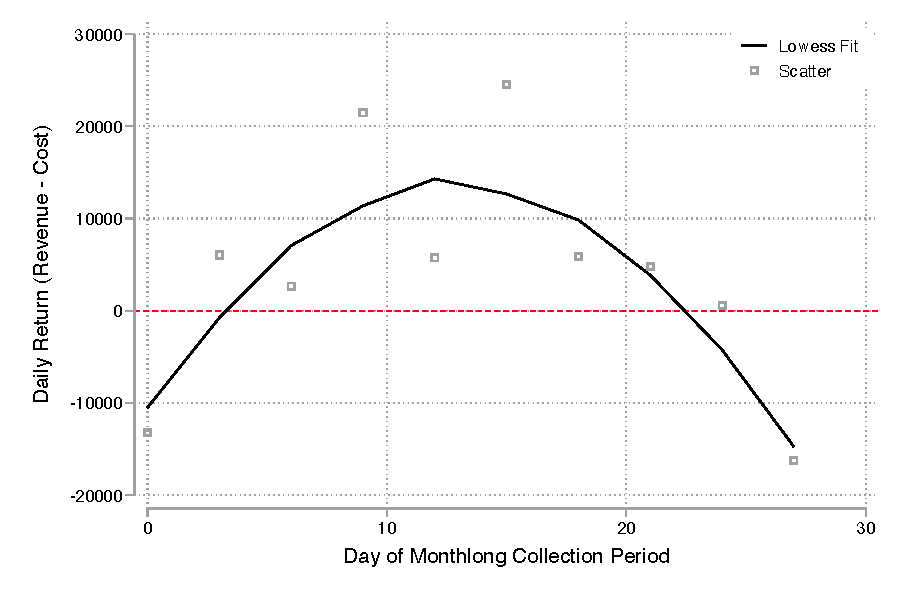
\includegraphics[scale=.75]{Output/return_by_day_central_month1-2_bin.pdf} \\
B: Return to Additional Visits \\
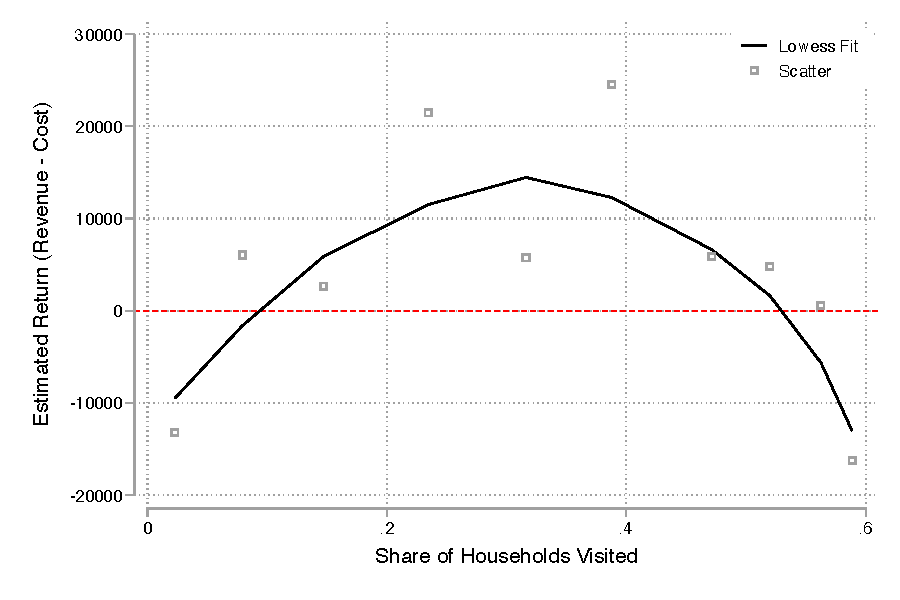
\includegraphics[scale=.75]{Output/return_by_visits_central_month1-2_bin.pdf}\end{tabular}
\end{center}
\usebox{\tablebox}\\[1ex]
\parbox{6in}{\footnotesize \textit{Notes}: This figure shows the estimated daily return on tax collection in Central (\textit{i}) over the course of the month in which collectors were assigned to a given neighborhood, and (\textit{ii}) as a function of the share of the total households in the neighborhood that were visited. The revenue data come from the handheld receipt printers and the timestamp recorded for each transaction. The cost data come from tax campaign records concerning transportation costs incurred by collectors. We discuss these results in Section \ref{info_adv}.}
\vspace{.5cm}
\end{figure}

%%%%%%%%%%%%%%%%%%%%%%%%%%%%%%%%%%%%%%%%%%%%%%%%%%%%%%%%%%%%%%%%%

\clearpage

%%%%%%%%%%%%%%%%%%%%%%%%%%%%%%%%%%%%%%%%%%%%%%%%%%%%%%%%%%%%%%%%%

\section{Additional Details on the Tax Campaign and its Evaluation}
\label{additional_campaign_details}

%%%%%%%%%%%%%%%%%%%%%%%%%%%%%%%%%%%%%%%%%%%%%%%%%%%%%%%%%%%%%%%%%

\FloatBarrier

%%%%%%%%%%%%%%%%%%%%%%%%%%%%%%%%%%%%%%%%%%%%%%%%%%%%%%%%%%%%%%%%%

\subsection{Block-Randomized Design}
\label{randomization}

%%%%%%%%%%%%%%%%%%%%%%%%%%%%%%%%%%%%%%%%%%%%%%%%%%%%%%%%%%%%%%%%%

\FloatBarrier

%%%%%%%%%%%%%%%%%%%%%%%%%%%%%%%%%%%%%%%%%%%%%%%%%%%%%%%%%%%%%%%%%

\subsection{Tax Letter Message Treatments}
\label{information_treatments}

%%%%%%%%%%%%%%%%%%%%%%%%%%%%%%%%%%%%%%%%%%%%%%%%%%%%%%%%%%%%%%%%%

\FloatBarrier

%%%%%%%%%%%%%%%%%%%%%%%%%%%%%%%%%%%%%%%%%%%%%%%%%%%%%%%%%%%%%%%%%

\subsection{Chief Jurisdiction Mapping}

\label{chief_selection}

%%%%%%%%%%%%%%%%%%%%%%%%%%%%%%%%%%%%%%%%%%%%%%%%%%%%%%%%%%%%%%%%%

\FloatBarrier

%%%%%%%%%%%%%%%%%%%%%%%%%%%%%%%%%%%%%%%%%%%%%%%%%%%%%%%%%%%%%%%%%

\subsection{Logistics Pilot}
\label{logistics_pilot}

%%%%%%%%%%%%%%%%%%%%%%%%%%%%%%%%%%%%%%%%%%%%%%%%%%%%%%%%%%%%%%%%%

\subsection{Time Imbalance}
\label{time_confound_appendix}

%%%%%%%%%%%%%%%%%%%%%%%%%%%%%%%%%%%%%%%%%%%%%%%%%%%%%%%%%%%%%%%%%

\subsubsection{Preferred Specification and Robustness Tests}

%%%%%%%%%%%%%%%%%%%%%%%%%%%%%%%%%%%%%%%%%%%%%%%%%%%%%%%%%%%%%%%%%

\FloatBarrier

%%%%%%%%%%%%%%%%%%%%%%%%%%%%%%%%%%%%%%%%%%%%%%%%%%%%%%%%%%%%%%%%%

\subsection{Detailed Survey-based Variable Descriptions}
\label{variable_descriptions}

%%%%%%%%%%%%%%%%%%%%%%%%%%%%%%%%%%%%%%%%%%%%%%%%%%%%%%%%%%%%%%%%%

\section{Further Analysis}


%%%%%%%%%%%%%%%%%%%%%%%%%%%%%%%%%%%%%%%%%%%

%%%%%%%%%%%%%%%%%%%%%%%%%%%%%%%%%%%%%%%%%%%%%%%%%%%%%%%%%%%%%%%%%

\subsection{Conceptual Framework}
\label{model}

%%%%%%%%%%%%%%%%%%%%%%%%%%%%%%%%%%%%%%%%%%%%%%%%%%%%%%%%%%%%%%%%%

\subsubsection{Setup}\label{model_setup}

%%%%%%%%%%%%%%%%%%%%%%%%%%%%%%%%%%%%%%%%%%%%%%%%%%%%%%%%%%%%%%%%%

\label{eq_avgprob}

%%%%%%%%%%%%%%%%%%%%%%%%%%%%%%%%%%%%%%%%%%%%%%%%%%%%%%%%%%%%%%%%%

\subsubsection{Collector's objective function}

\label{collector_OF}

%%%%%%%%%%%%%%%%%%%%%%%%%%%%%%%%%%%%%%%%%%%%%%%%%%%%%%%%%%%%%%%%%

\subsubsection{Government's Decision}

%%%%%%%%%%%%%%%%%%%%%%%%%%%%%%%%%%%%%%%%%%%%%%%%%%%%%%%%%%%%%%%%%

\label{govt_OF}

%%%%%%%%%%%%%%%%%%%%%%%%%%%%%%%%%%%%%%%%%%%%%%%%%%%%%%%%%%%%%%%%%

\label{govt_constraints} 

%%%%%%%%%%%%%%%%%%%%%%%%%%%%%%%%%%%%%%%%%%%%%%%%%%%%%%%%%%%%%%%%%

\subsubsection{Discussion}

%%%%%%%%%%%%%%%%%%%%%%%%%%%%%%%%%%%%%%%%%%%%%%%%%%%%%%%%%%%%%%%%%

\subsubsection{External Validity}\label{external_validity_model}

%%%%%%%%%%%%%%%%%%%%%%%%%%%%%%%%%%%%%%%%%%%%%%%%%%%%%%%%%%%%%%%%%

\begin{figure}[H]\caption{Example of Potential Taxpayers by Collector Type}\label{lambda}
\centering
\scalebox{0.8}{\begin{tikzpicture}
\begin{axis}[
  no markers, domain=0:10, samples=100,
  axis lines*=left, xlabel=$\lambda$, ylabel=$f(\lambda)$,
  every axis y label/.style={at=(current axis.above origin),anchor=south},
  every axis x label/.style={at=(current axis.right of origin),anchor=west},
  height=7cm, width=16cm,
  xtick=\empty, ytick=\empty,
  enlargelimits=false, clip=false, axis on top,
  grid = major
  ]
  \addplot [fill=gray!20, draw=none, domain=5.9:7] {gauss(4,1)} \closedcycle;
    \addplot [fill=cyan!50!gray!20, draw=none, domain=8:10] {gauss(6.75,1)} \closedcycle;
  \addplot [very thick,gray!60!black,domain=0:6.25] {gauss(4,1)} node[above] {$\hspace{6ex}f(\lambda_C)$};
  \addplot [very thick,cyan!50!black,domain=0:9] {gauss(6.75,1)} node[above] {$\hspace{6ex}f(\lambda_L)$};
  \addplot [very thick,gray!60!black,domain=6.25:10] {gauss(4,1)};
  \addplot [very thick,cyan!50!black,domain=9:10] {gauss(6.75,1)};

\coordinate (x2) at (800,400);
\coordinate (x1) at (800,0);
\coordinate (x5) at (590,400);
\coordinate (x6) at (590,0);

\draw[thick, dashed] (x2) -- (x1) node[below] {$\rho_L$};
\draw[thick, dashed] (x5) -- (x6) node[below] {$\rho_C$};
\end{axis}
\end{tikzpicture}}
\usebox{\tablebox}\\[1ex]
\parbox{6in}{\footnotesize \textit{Notes:} Curves $f(\lambda_L)$ and $f(\lambda_C)$ are the distribution of intrinsic willingness, $\rho_L$ and $\rho_C$ the cost of non-compliance, and shaded areas proportion of potential payers by collector type $L$ and $C$. This figure is discussed in Section \ref{persuasion} and \ref{model_setup}.}
\end{figure}

%%%%%%%%%%%%%%%%%%%%%%%%%%%%%%%%%%%%%%%%%%%%%%%%%%%%%%%%%%%%%%%%%

\begin{figure}[H]\caption{Average Probability of Payment by Visits and Collector Type}\label{avgprob}
\centering
\scalebox{0.8}{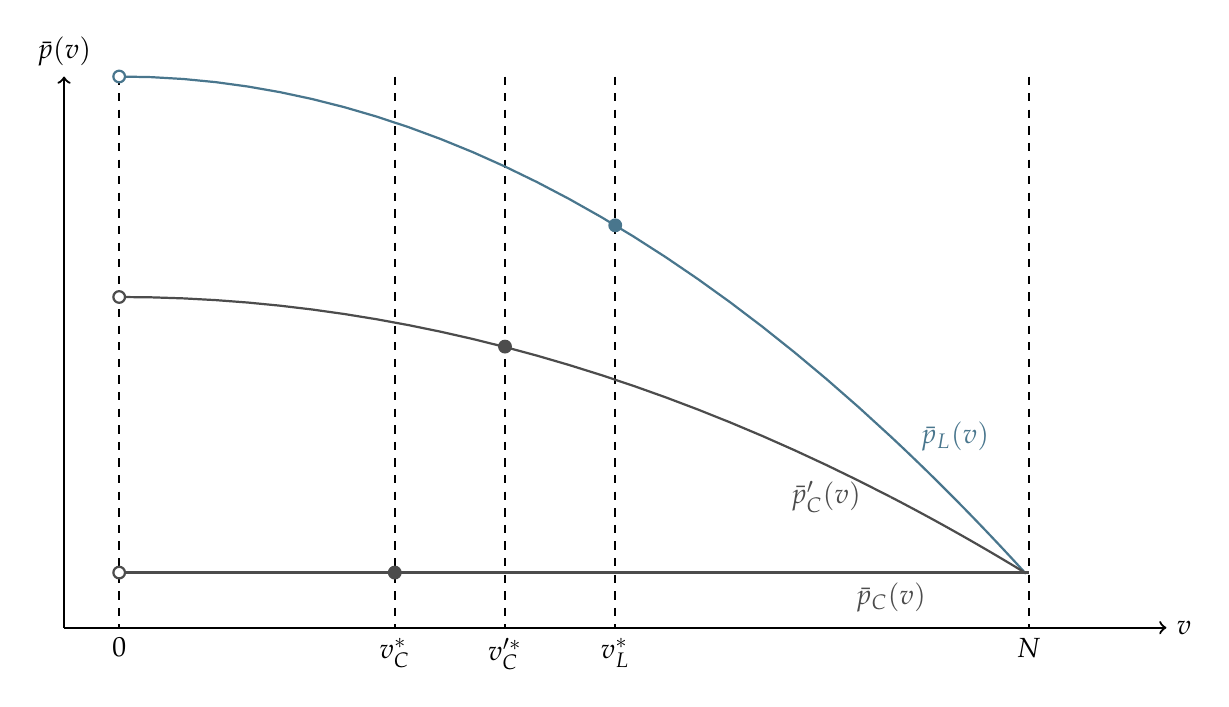
\begin{tikzpicture}[domain=0:100,range=0:200,scale=0.7,thick]
\usetikzlibrary{calc}

\def\inc{10}
\def\pa{1}
\def\pb{1}
\def\panew {0.5}

\coordinate (x2) at (10,10);
\coordinate (x1) at (10,0);
\coordinate (x3) at (0,5);
\coordinate (x4) at (20,5);
\coordinate (x5) at (17.5,10);
\coordinate (x6) at (17.5,0);
\coordinate (x7) at (1,10);
\coordinate (x8) at (1,0);
\coordinate (x9) at (8,10);
\coordinate (x10) at (8,0);
\coordinate (x11) at (6,10);
\coordinate (x12) at (6,0);
\coordinate (p1) at (1,1);
\coordinate (p2) at (1,6);
\coordinate (p3) at (1,10);
\coordinate (p4) at (10,10);

\draw[->] (0,0) -- (20,0) node[right] {$v$};
\draw[->] (0,0) -- (0,10) node[above] {$\bar{p}(v)$};
\draw[thick, dashed] (x2) -- (x1) node[below] {$v^*_L$};
\draw[thick, dashed] (x9) -- (x10) node[below] {$v'^*_C$};
\draw[thick, dashed] (x11) -- (x12) node[below] {$v^*_C$};
\draw[thick, dashed] (x5) -- (x6) node[below] {$N$};
\draw[thick, dashed] (x7) -- (x8) node[below] {$0$};

\draw[thick,color=cyan!50!black,domain=1:15] plot (\x,{(-(\x-1)^2)/30+10}) node[right] {$\hspace{1.5ex}\bar{p}_L(v)$};
\draw[thick,color=gray!60!black,domain=1:15] plot(\x,{1}) node[below] {$\bar{p}_C(v)$};
\draw[thick,color=gray!60!black,domain=1:15] plot (\x,{(-(\x-1)^2)/54+6}) node[left] {$\bar{p}_C'(v)\hspace{1.5ex}$};
\draw[thick,color=cyan!50!black,domain=15:17.45] plot (\x,{(-(\x-1)^2)/30+10});
\draw[thick,color=gray!60!black,domain=15:17.5] plot(\x,{1}) ;
\draw[thick,color=gray!60!black,domain=15:17.45] plot (\x,{(-(\x-1)^2)/54+6});

\filldraw[color=gray!60!black,fill=white] (p1) circle (3 pt);
\filldraw[color=gray!60!black,fill=white] (p2) circle (3 pt);
\filldraw[color=cyan!50!black,fill=white] (p3) circle (3 pt);

\filldraw[color=gray!60!black,fill=gray!60!black] (6,1) circle (3 pt);
\filldraw[color=gray!60!black,fill=gray!60!black] (8,5.1) circle (3 pt);
\filldraw[color=cyan!50!black,fill=cyan!50!black] (10,7.3) circle (3 pt);
\end{tikzpicture}}
\usebox{\tablebox}\\[1ex]
\parbox{6in}{\footnotesize \textit{Notes:} Curves $\bar{p}_L(v)$, $\bar{p}_C(v)$, and $\bar{p}_C'(v)$ are the average probability of payment among visited property owners by collector type and informedness.  $v^*_k$ are the optimal number of visits selected by collectors, $N$ is the total number of property owners.  This figure displays the case where $E[\lambda_L]=E[\lambda_C]$ and $\rho_L=\rho_C$: the only difference across collector types in average payment probability derives from the level of information about $\lambda_i$'s of property owners and number of properties visited. We discuss this figure in Section \ref{info_adv} and \ref{model_setup}.}
\end{figure}

%%%%%%%%%%%%%%%%%%%%%%%%%%%%%%%%%%%%%%%%%%%%%%%%%%%%%%%%%%%%%%%%%

\clearpage

%%%%%%%%%%%%%%%%%%%%%%%%%%%%%%%%%%%%%%%%%%%%%%%%%%%%%%%%%%%%%%%%%
 
\subsection{Combined Team --- Central X Local}
\label{cxl_discussion}

%%%%%%%%%%%%%%%%%%%%%%%%%%%%%%%%%%%%%%%%%%%%%%%%%%%%%%%%%%%%%%%%%

\begin{figure}[H]
\textbf{\caption{Decreasing compliance over time --- Central, Local, CXL \label{all_tmts_overtime_bubbles_withCXL}}}
\centering
\scalebox{0.95}{
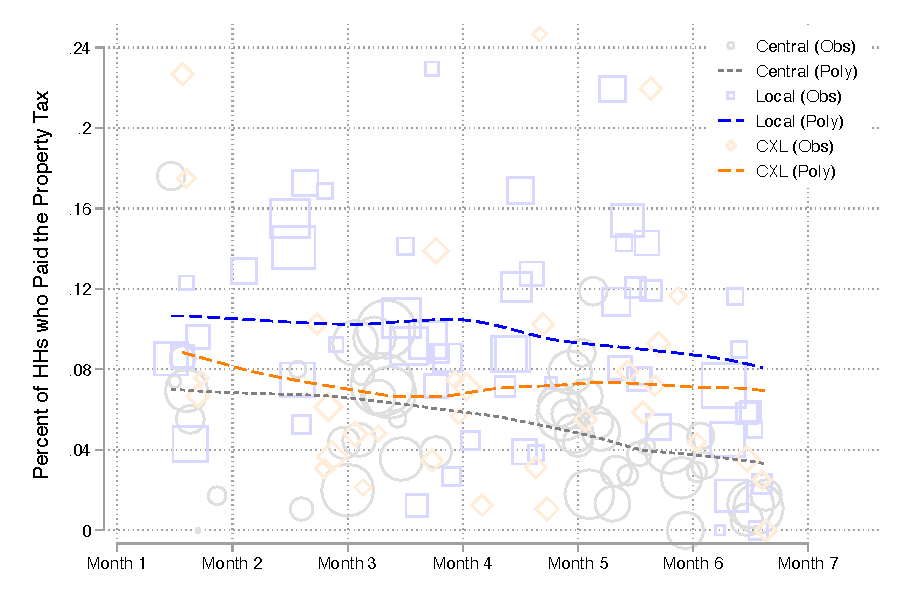
\includegraphics[scale=0.75]{Output/compliance_over_time_CXL.pdf}
}
\caption*{\footnotesize{\upshape{\textnormal{\textit{Notes}: This figure shows the decrease in compliance for Central, Local, and CLI over the tax campaign. Blue squares represent Local observations, gray circles represent Central observations, and orange diamonds represent CXL observations, with size indicating number of observations.  Lines --- dashed blue for Local, dotted gray for Central, and dashed orange for CXL (Panel B) --- are local linear polynomials estimated using the displayed data, separately by treatment.}}}}
\end{figure}

%%%%%%%%%%%%%%%%%%%%%%%%%%%%%%%%%%%%%%%%%%%%%%%%%%%%%%%%%%%%%%%%%

\begin{table}[H]
\textbf{\caption{\label{Table_CvCXL} Central v. Central X Local}}
\centering
\begin{lrbox}{\tablebox}

\resizebox{15cm}{!}{
{
\def\sym#1{\ifmmode^{#1}\else\(^{#1}\)\fi}
\begin{tabular}{l*{6}{c}}
\hline\hline
                &\multicolumn{1}{c}{Tax Compliance}&\multicolumn{5}{c}{Tax Amount}                                                                \\
                &\multicolumn{1}{c}{(1)}         &\multicolumn{1}{c}{(2)}         &\multicolumn{1}{c}{(3)}         &\multicolumn{1}{c}{(4)}         &\multicolumn{1}{c}{(5)}         &\multicolumn{1}{c}{(6)}         \\
\hline
Central X Local &    0.018\sym{*}  &  -10.647         &    0.019         &    0.065         &    0.029\sym{**} &    0.013         \\
                &  (0.010)         & (27.683)         &  (0.037)         &  (0.061)         &  (0.014)         &  (0.010)         \\
Local           &                  &                  &                  &                  &                  &    0.044\sym{***}\\
                &                  &                  &                  &                  &                  &  (0.007)         \\
Time FE         &      Yes         &      Yes         &      Yes         &      Yes         &      Yes         &      Yes         \\
House FE        &      Yes         &      Yes         &      Yes         &      Yes         &      Yes         &      Yes         \\
Stratum FE      &      Yes         &      Yes         &      Yes         &      Yes         &      Yes         &      Yes         \\
\hline
Observations    &    18211         &    18211         &    12476         &    12464         &     5030         &    32496         \\
Clusters        &      142         &      142         &      141         &      141         &      140         &      252         \\
Mean            &     .053         &  156.773         &     .396         &     .518         &     .102         &     .053         \\
CXLvC\_p         &                  &                  &                  &                  &                  &                  \\
\hline\hline
\end{tabular}
}

}
\end{lrbox}
\usebox{\tablebox}\\[1ex]
\parbox{6in}{\footnotesize \textit{Notes}: This table compares the Central X Local (CXL) arm to the Central arm, which is the excluded category. Columns 1, 5, and 6 report impacts on compliance. Column 2 reports impacts on revenues. Columns 3 and 4 report differences in tax visits by collectors after registration by the extensive and intensive margins, respectively. All regressions include fixed effects for house type, randomization strata, and time periods and cluster standard errors at the neighborhood level. All specifications include time fixed effects defined to maximize overlap between the treatments under comparison, as discussed in Section \ref{estimation}. Column 5 restricts to the subsample of properties that received any tax visits after registration. Column 6 includes a dummy for the Local treatment in the regression. The bottom row reports the $p$-value from a test for equality between the CXL and Local. We discuss these results in Section \ref{cxl_discussion}.}
\end{table}

%%%%%%%%%%%%%%%%%%%%%%%%%%%%%%%%%%%%%%%%%%%%%%%%%%%%%%%%%%%%%%%%%

\subsection{State Collector Team Composition and Performance}
\label{team_composition}

%%%%%%%%%%%%%%%%%%%%%%%%%%%%%%%%%%%%%%%%%%%%%%%%%%%%%%%%%%%%%%%%%

\begin{table}[H]
\vspace{.5cm}
\textbf{\caption{State Collector Performance by Team Composition \label{c_cli_team_composition}}}
\centering
\centerfloat
\scalebox{.6}{
{
\def\sym#1{\ifmmode^{#1}\else\(^{#1}\)\fi}
\begin{tabular}{l*{12}{c}}
\hline\hline
                &\multicolumn{3}{c}{Tax Compliance - Similarity}         &\multicolumn{3}{c}{Tax Compliance - Distance}           &\multicolumn{3}{c}{Tax Revenue - Similarity}            &\multicolumn{3}{c}{Tax Revenue - Distance}              \\
                &\multicolumn{1}{c}{(1)}         &\multicolumn{1}{c}{(2)}         &\multicolumn{1}{c}{(3)}         &\multicolumn{1}{c}{(4)}         &\multicolumn{1}{c}{(5)}         &\multicolumn{1}{c}{(6)}         &\multicolumn{1}{c}{(7)}         &\multicolumn{1}{c}{(8)}         &\multicolumn{1}{c}{(9)}         &\multicolumn{1}{c}{(10)}         &\multicolumn{1}{c}{(11)}         &\multicolumn{1}{c}{(12)}         \\
\hline
(max) age\_similar&    0.029\sym{**} &                  &                  &                  &                  &                  &   40.800         &                  &                  &                  &                  &                  \\
                &  (0.011)         &                  &                  &                  &                  &                  & (33.746)         &                  &                  &                  &                  &                  \\
(max) educ\_similar&                  &   -0.004         &                  &                  &                  &                  &                  &    8.346         &                  &                  &                  &                  \\
                &                  &  (0.013)         &                  &                  &                  &                  &                  & (33.983)         &                  &                  &                  &                  \\
(max) inc\_mo\_similar&                  &                  &    0.014         &                  &                  &                  &                  &                  &   -5.483         &                  &                  &                  \\
                &                  &                  &  (0.012)         &                  &                  &                  &                  &                  & (37.411)         &                  &                  &                  \\
(max) age\_dist  &                  &                  &                  &   -0.001         &                  &                  &                  &                  &                  &   -0.658         &                  &                  \\
                &                  &                  &                  &  (0.001)         &                  &                  &                  &                  &                  &  (2.702)         &                  &                  \\
(max) educ\_dist &                  &                  &                  &                  &    0.001         &                  &                  &                  &                  &                  &    1.102         &                  \\
                &                  &                  &                  &                  &  (0.002)         &                  &                  &                  &                  &                  &  (5.607)         &                  \\
(max) inc\_mo\_dist&                  &                  &                  &                  &                  &    0.000         &                  &                  &                  &                  &                  &   -0.094         \\
                &                  &                  &                  &                  &                  &  (0.000)         &                  &                  &                  &                  &                  &  (0.334)         \\
Stratum FE      &      Yes         &      Yes         &      Yes         &      Yes         &      Yes         &      Yes         &      Yes         &      Yes         &      Yes         &      Yes         &      Yes         &      Yes         \\
\hline
Observations    &      187         &      187         &      187         &      187         &      187         &      187         &      187         &      187         &      187         &      187         &      187         &      187         \\
\hline\hline
\end{tabular}
}

}
\usebox{\tablebox}\\[1ex]
\parbox{6in}{\footnotesize \textit{Notes}: This table examines the relationship between state collector team structure and tax compliance (Columns 1--6) or tax revenue (Columns 7--12) at the neighborhood level. The variable \textit{Similarity} is a dummy for the two randomly assigned collectors both lying either above or below the median in the collector trait noted in the column titles. \textit{Distance} is the absolute value of the difference between both collectors' traits, measured in years for age and level of education (Columns 1--2, 4--5, 7--8, and 10--11) and in dollars for income (Columns 3, 6, 9, and 12). All regressions include stratum fixed effects, and robust standard errors. In addition, we  control for the average level of the corresponding trait for the assigned collectors in each neighborhood. The sample includes all neighborhoods assigned to Central and CLI, i.e., where state collectors were randomly assigned.}
\end{table}

%%%%%%%%%%%%%%%%%%%%%%%%%%%%%%%%%%%%%%%%%%%%%%%%%%%%%%%%%%%%%%%%%

\FloatBarrier

%%%%%%%%%%%%%%%%%%%%%%%%%%%%%%%%%%%%%%%%%%%%%%%%%%%%%%%%%%%%%%%%%

\subsection{Collector Exhaustion and Demoralization}
\label{demoralization}

%%%%%%%%%%%%%%%%%%%%%%%%%%%%%%%%%%%%%%%%%%%%%%%%%%%%%%%%%%%%%%%%%

\begin{table}[ht]
\textbf{\caption{Local v. Central: Visits over Time \label{TimeInteraction}}}
\centering
\scalebox{1}{
{
\def\sym#1{\ifmmode^{#1}\else\(^{#1}\)\fi}
\begin{tabular}{l*{2}{c}}
\hline\hline
                &\multicolumn{1}{c}{Visited}&\multicolumn{1}{c}{N Visits}\\
                &\multicolumn{1}{c}{(1)}         &\multicolumn{1}{c}{(2)}         \\
\hline
Local           &   -0.165\sym{**} &   -0.187\sym{**} \\
                &  (0.052)         &  (0.093)         \\
Local X Time Decile&    0.029\sym{***}&    0.036\sym{**} \\
                &  (0.009)         &  (0.015)         \\
Time Decile     &   -0.031\sym{***}&   -0.042\sym{***}\\
                &  (0.005)         &  (0.009)         \\
House FE        &      Yes         &      Yes         \\
Stratum FE      &      Yes         &      Yes         \\
\hline
Observations    &    18382         &    18371         \\
Clusters        &      212         &      212         \\
Mean            &     .417         &     .552         \\
\hline\hline
\end{tabular}
}

}
\parbox{\textwidth}{\footnotesize{\textit{Notes}: This table examines visits from tax collector on the extensive (Column 1) and intensive (Column 2) margin across treatments and over time. Specifically, we take deciles of the time distribution of the tax campaign, and interact these with the Local treatment dummy. All regressions include stratum and house type fixed effects, and cluster standard errors at the neighborhood level.}}
\end{table}

%%%%%%%%%%%%%%%%%%%%%%%%%%%%%%%%%%%%%%%%%%%%%%%%%%%%%%%%%%%%%%%%%

\begin{table}[ht]
\vspace{.5cm}
\textbf{\caption{Investigating Collector Demoralization and Exhaustion \label{compliance_demoral_altsamp}}}
\centering
\scalebox{1}{
\tiny{{
\def\sym#1{\ifmmode^{#1}\else\(^{#1}\)\fi}
\begin{tabular}{l*{6}{c}}
\hline\hline
                &\multicolumn{1}{c}{Tax Compliance}&\multicolumn{1}{c}{Tax Compliance}&\multicolumn{1}{c}{Tax Compliance}&\multicolumn{1}{c}{Tax Compliance}&\multicolumn{1}{c}{Tax Compliance}&\multicolumn{1}{c}{Tax Compliance}\\
                &\multicolumn{1}{c}{(1)}         &\multicolumn{1}{c}{(2)}         &\multicolumn{1}{c}{(3)}         &\multicolumn{1}{c}{(4)}         &\multicolumn{1}{c}{(5)}         &\multicolumn{1}{c}{(6)}         \\
\hline
Local           &    0.035\sym{***}&    0.032\sym{***}&    0.047\sym{**} &    0.051\sym{***}&    0.051\sym{***}&    0.056\sym{***}\\
                &  (0.008)         &  (0.009)         &  (0.016)         &  (0.013)         &  (0.011)         &  (0.013)         \\
CLI             &                  &    0.024\sym{**} &                  &    0.023\sym{**} &                  &    0.034\sym{**} \\
                &                  &  (0.009)         &                  &  (0.009)         &                  &  (0.013)         \\
Time FE         &      Yes         &      Yes         &      Yes         &      Yes         &      Yes         &      Yes         \\
House FE        &      Yes         &      Yes         &      Yes         &      Yes         &      Yes         &      Yes         \\
Stratum FE      &      Yes         &      Yes         &      Yes         &      Yes         &      Yes         &      Yes         \\
\hline
Observations    &    16642         &    26064         &    13049         &    22471         &    16505         &    25927         \\
Clusters        &      130         &      210         &      100         &      180         &      129         &      209         \\
Mean            &     .052         &     .052         &     .052         &     .052         &     .057         &     .057         \\
\hline\hline
\end{tabular}
}
}
}
\parbox{\textwidth}{\footnotesize{\textit{Notes}: This table reports estimates from Equation 1, comparing property tax compliance in Local and CLI to Central (the excluded category). All regressions include fixed effects for randomization strata, house type, and time period fixed effects and cluster standard errors at the neighborhood level. Columns 1--2 restrict the Local sample to neighborhoods where chiefs in charge of collection worked in multiple neighborhoods. Columns 3--4 restrict the Local sample to neighborhoods with chiefs who worked in multiple months (in different neighborhoods), keeping only neighborhoods in their second collection period. Columns 5--6 restrict the Central sample to neighborhoods with state agents collecting for the first time.  The data include all properties registered by tax collectors merged with the government's property tax database.}}
\end{table}

%%%%%%%%%%%%%%%%%%%%%%%%%%%%%%%%%%%%%%%%%%%%%%%%%%%%%%%%%%%%%%%%%

\begin{table}[ht]
\textbf{\caption{Central: Exposure to Central + Local Information \label{CLIexposure}}}
\centering
\scalebox{1}{
{
\def\sym#1{\ifmmode^{#1}\else\(^{#1}\)\fi}
\begin{tabular}{l*{4}{c}}
\hline\hline
                &\multicolumn{1}{c}{Compliance}&\multicolumn{1}{c}{Compliance}&\multicolumn{1}{c}{Revenues}&\multicolumn{1}{c}{Revenues}\\
                &\multicolumn{1}{c}{(1)}         &\multicolumn{1}{c}{(2)}         &\multicolumn{1}{c}{(3)}         &\multicolumn{1}{c}{(4)}         \\
\hline
Post CLI Exposure&   -0.017         &    0.012         & -126.423         &    8.685         \\
                &  (0.075)         &  (0.018)         &(168.455)         & (36.417)         \\
Local Trend (Compliance)&    1.293         &    2.032\sym{**} &                  &                  \\
                &  (2.258)         &  (0.920)         &                  &                  \\
Local Trend (Revenues)&                  &                  &    0.148         &    1.510\sym{**} \\
                &                  &                  &  (2.029)         &  (0.755)         \\
House FE        &      Yes         &      Yes         &      Yes         &      Yes         \\
Period FE       &       No         &      Yes         &       No         &      Yes         \\
\hline
Observations    &     6447         &    14164         &     6447         &    14164         \\
Clusters        &       52         &       84         &       52         &       84         \\
Mean            &      .12         &     .085         &  319.104         &   234.09         \\
\hline\hline
\end{tabular}
}

}
\parbox{\textwidth}{\footnotesize{\textit{Notes}: This table reports changes in compliance and revenues within the Central treatment arm, comparing outcomes before Central agents engaged in consultation with chiefs in the CLI arm with those after consultations took place, for the same set of Central agents. We examine two periods: changes in outcomes between months 1 and 3 (for collectors working in the CLI arm in month 2), and between months 3 and 5 (for collectors working in the CLI arm in month 4).  We exclude the period straddling the final month of CLI (months 5 and 7), as there are few neighborhoods assigned to the Local treatment arm in month 7.  In each period, we estimate the compliance trend in the Local treatment arm and control for it when comparing the pre- and post-periods in the Central treatment arm.  All regressions include house type fixed effects.  When considering multiple periods we include period fixed effects corresponding to the above-described periods.  We do not include fixed effects for stratum or collectors as collectors rotate (due to random assignment to neighborhoods) to different strata and collection partners and thus including these fixed effects would result in a severely restricted sample.}}
\end{table}

%%%%%%%%%%%%%%%%%%%%%%%%%%%%%%%%%%%%%%%%%%%%%%%%%%%%%%%%%%%%%%%%%

\begin{table}[ht]
\textbf{\caption{Local v. Central: Endline Differences in Collector Characteristics \label{endline_collector_traits}}}
\centering
\scalebox{1}{
{\def\sym#1{\ifmmode^{#1}\else\(^{#1}\)\fi} \begin{tabular}{l*{4}{c}} \hline\hline 
& beta & SE & R2 & N \\
Extrinsic motivation & -0.092 & 0.222 & 0.002 & 111.000 \\
Intrinsic motivation & -0.308 & 0.225 & 0.017 & 111.000 \\
Introjection & 0.089 & 0.218 & 0.002 & 111.000 \\
Goal orientation & -0.235 & 0.212 & 0.011 & 111.000 \\
Amotivation & 0.486 & 0.218 & 0.044 & 111.000 \\
Conscientiousness (big 5) & -0.132 & 0.239 & 0.003 & 111.000 \\
Extroverted (big 5) & -0.384 & 0.226 & 0.026 & 111.000 \\
Discount factor & -0.106 & 0.215 & 0.002 & 111.000 \\
Optimism & 0.205 & 0.216 & 0.008 & 111.000 \\
Locus of Control & 0.232 & 0.195 & 0.013 & 111.000 \\
Persistence (maze) & 0.727 & 0.209 & 0.122 & 89.000 \\
Dishonesty/cheating (RAG) & -0.222 & 0.213 & 0.010 & 111.000 \\
\hline\hline \end{tabular} }

}
\parbox{\textwidth}{\footnotesize{\textit{Notes}: This table examines endline differences in collector motivation and personality traits using data from a survey conducted with all collectors after the tax campaign. Each row summarizes a regression of the variable noted on an indicator for chiefs who worked in Local (with the omitted category of state collectors who worked in Central). All dependent variables are standardized to facilitate interpretation of magnitudes. The motivation indices in Panel A come from the psychology literature \citep{tremblay2009}. The Big 5 indices come from \cite{borghans2008}. Locus of control questions come from the World Values Survey. The persistence measure is the total number of minutes the collector worked on an impossible maze. The dishonesty/cheating measure involves allocating money between oneself and a payoff to the government according to die rolls, as explained in detail in \cite{lowes2017}.}}
\end{table}

%%%%%%%%%%%%%%%%%%%%%%%%%%%%%%%%%%%%%%%%%%%%%%%%%%%%%%%%%%%%%%%%%

\begin{table}[ht]
\vspace{.5cm}
\textbf{\caption{Local v. Central: Endline Amotivation \label{amotivation}}}
\centering
\scalebox{01}{
{
\def\sym#1{\ifmmode^{#1}\else\(^{#1}\)\fi}
\begin{tabular}{l*{4}{c}}
\hline\hline
                &\multicolumn{1}{c}{(1)}         &\multicolumn{1}{c}{(2)}         &\multicolumn{1}{c}{(3)}         &\multicolumn{1}{c}{(4)}         \\
\hline
Local           &    0.187         &    0.136         &    0.651\sym{**} &    0.486\sym{**} \\
                &  (0.214)         &  (0.217)         &  (0.212)         &  (0.218)         \\
\hline
Observations    &      111         &      111         &      111         &      111         \\
Mean            &     .161         &     .094         &     .484         &     .369         \\
\hline\hline
\end{tabular}
}

}
\parbox{\textwidth}{\footnotesize{\textit{Notes}: This table examines endline differences in collector amotivation using data from a survey conducted with all collectors after the tax campaign. The survey questions were drawn from \cite{tremblay2009}.}}
\vspace{.5cm}
\end{table}

%%%%%%%%%%%%%%%%%%%%%%%%%%%%%%%%%%%%%%%%%%%%%%%%%%%%%%%%%%%%%%%%%

\FloatBarrier

%%%%%%%%%%%%%%%%%%%%%%%%%%%%%%%%%%%%%%%%%%%%%%%%%%%%%%%%%%%%%%%%%

\subsection{Quantifying the Knowledge Gap between Chiefs and State Agents}
\label{knowledge_quiz}

%%%%%%%%%%%%%%%%%%%%%%%%%%%%%%%%%%%%%%%%%%%%%%%%%%%%%%%%%%%%%%%%%

\begin{figure}[H]
\textbf{\caption{Knowledge Quiz: State Collectors v. Non-Collector Chiefs  \label{C_L_knowledge}}}
\centering
\begin{tabular}{cc}
\\
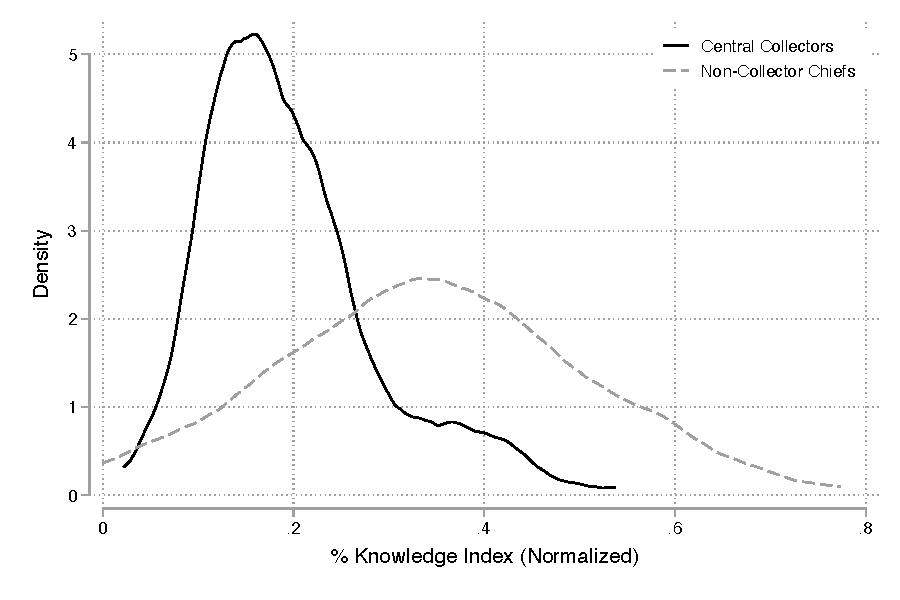
\includegraphics[scale=1]{Output/KnowsIndex_C_vs_L_NonCollectorChiefs.pdf}
\end{tabular}
\parbox{\textwidth}{\footnotesize{\upshape{\textnormal{\textit{Notes}: This figure shows the distributions of knowledge about citizens for chiefs compared to state collectors. Knowledge of the inhabitants of the neighborhood is measured by the percentage of correct answers regarding a random sample of property owners in a short quiz-type survey module conducted after tax collection. Questions included the owner's name, education level, and occupation. Chiefs took quizzes for their own neighborhoods, but we restrict the sample to chiefs who did not collect taxes (since the quiz was administered after the campaign); central agents took quizzes for randomly selected neighborhoods to simulate the knowledge they would have if assigned to a location before collecting taxes there. We discuss these results in Section \ref{info_adv}.}}}}
\end{figure}

%%%%%%%%%%%%%%%%%%%%%%%%%%%%%%%%%%%%%%%%%%%%%%%%%%%%%%%%%%%%%%%%%

\subsection{The Limits to Codifying Local Information} 
\label{codifiability}

%%%%%%%%%%%%%%%%%%%%%%%%%%%%%%%%%%%%%%%%%%%%%%%%%%%%%%%%%%%%%%%%%

\begin{figure}[H]
\centering{}\caption{Timing of Tax Collections by Treatment \label{time_collection_CvLvCLI.pdf}}
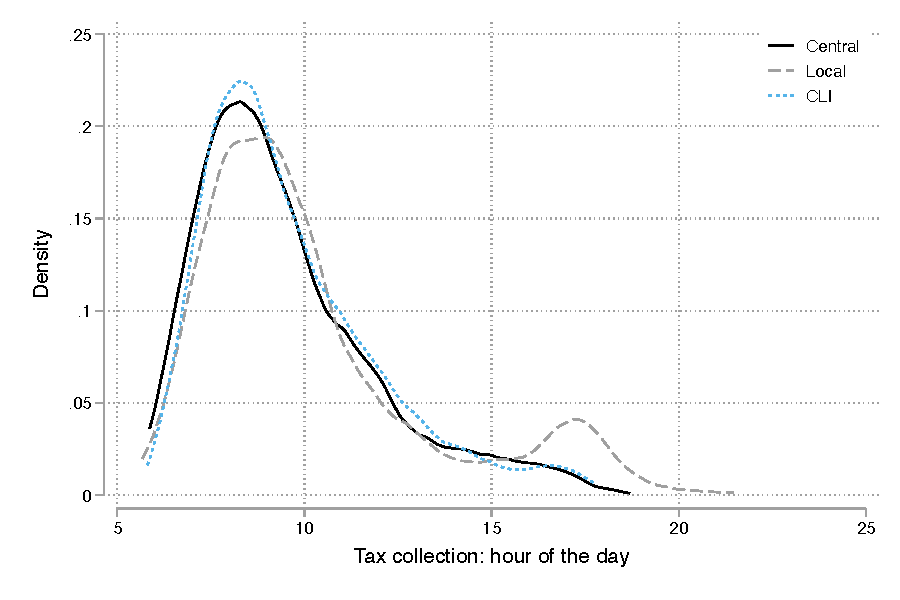
\includegraphics[scale=0.9]{Output/time_collection_CvLvCLI.pdf}
\usebox{\tablebox}\\[1ex]
\parbox{6in}{\footnotesize \textit{Notes}: This figure shows the distribution of tax payments according to the receipt data. We discuss these findings in Section \ref{info_adv}.}
\end{figure}

%%%%%%%%%%%%%%%%%%%%%%%%%%%%%%%%%%%%%%%%%%%%%%%%%%%%%%%%%%%%%%%%%

\subsection{Cost-Effectiveness}
\label{cost_effectiveness}

%%%%%%%%%%%%%%%%%%%%%%%%%%%%%%%%%%%%%%%%%%%%%%%%%%%%%%%%%%%%%%%%%

\begin{figure}[H]
\centering{}\caption{Costs and cost-effectiveness across treatments \label{fig:costs_all}}
\begin{tabular}{c}
A: Costs of Tax Collection Methods \\
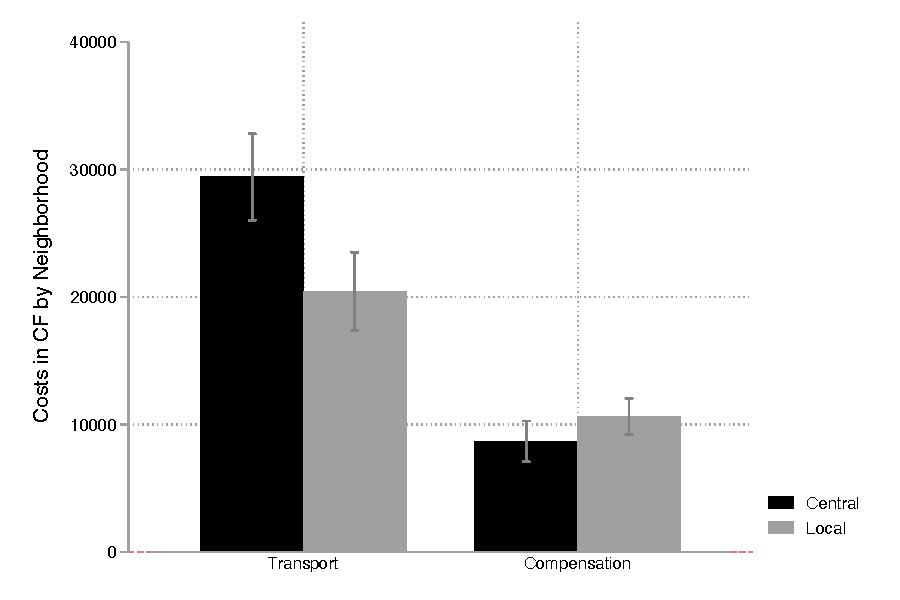
\includegraphics[scale=.8]{Output/costs_by_treatment.pdf} \\
\\
B: Cost-Effectiveness of Tax Collection Methods  \\
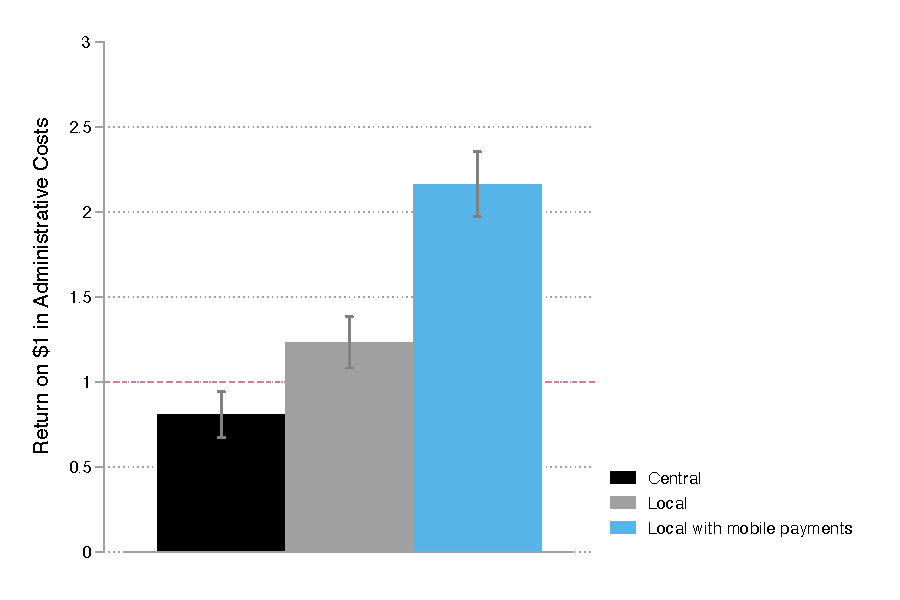
\includegraphics[scale=.8]{Output/Appdx_PaperFigure_marginal_revenue_hypothetical.pdf}\\
\end{tabular}
\parbox{6in}{\footnotesize \textit{Notes}: This figure reports estimated costs (Panel A) and cost-effectiveness (Panel B) for the Central and Local treatments. In Panel A, costs are broken down by transport and compensation. In Panel B, cost-effectiveness is the return of an additional \$1 spent on collection in particular treatment, and the hypothetical cost-effectiveness of Local with mobile payments is shown at far right. Estimates are the mean value of each measure averaging across neighborhoods.  Confidence intervals are shown by the vertical bars. We discuss these results in Section \ref{cost_effectiveness}.}
\end{figure}

%%%%%%%%%%%%%%%%%%%%%%%%%%%%%%%%%%%%%%%%%%%%%%%%%%%%%%%%%%%%%%%%%

\begin{figure}[H]
\centering{}\caption{Cost-effectiveness of Local and Central by Remoteness \label{cea_remoteness}}
\includegraphics[scale=.8]{Output/scatter_benefit_cost_dist_center_CvsL.pdf}
\parbox{6in}{\footnotesize \textit{Notes}: This figure reports estimated cost-effectiveness for the Central and Local treatments as a function of the distance from downtown Kananga. We discuss these results in Section \ref{cost_effectiveness}.}
\end{figure}

%%%%%%%%%%%%%%%%%%%%%%%%%%%%%%%%%%%%%%%%%%%%%%%%%%%%%%%%%%%%%%%%%

\begin{table}[H]
\vspace*{-1cm}
\textbf{\caption{\label{bribe_multiplier} Local v. Central: Bribe Multiplier}}
\centering
\begin{lrbox}{\tablebox}
\resizebox{15cm}{!}{
\csvautotabular[respect underscore=true]{Output/bribe_multiplier.csv}
}
\end{lrbox}
\usebox{\tablebox}\\[1ex]
\parbox{6in}{\footnotesize \textit{Notes}: This table reports measures from the tax campaign of total revenues collected and costs incurred for the Central and Local treatment arms. Columns 1 and 4 report revenues collected by treatment arm. Columns 2 and 5 report costs, which include bonuses paid to tax collectors and compensation  for transportation.  The second row reports costs under a hypothetical system in which chief collectors were paid (and remit tax collections) via mobile money rather than visiting the tax ministry to receive bonuses (and deposit collections). Costs for Central under this alternative system would remain the same. Columns 3 and 6 show the amounts of bribes collecting according to the measure at endline, scaled by the number of individuals surveyed at endline relative to the neighborhood population of households.  All amounts are in Congolese Francs.  Column 7 reports the implied multiplier on bribe payments that would be required for the government to weakly prefer employing state collectors instead of chief collectors: $\Gamma=((R_L-R_C)-(C_L-C_C))/(B_L-B_C)$. This formula is discussed in more detail in Section \ref{model_setup}. We discuss these results in Section \ref{cost_effectiveness}.}
\end{table}

%%%%%%%%%%%%%%%%%%%%%%%%%%%%%%%%%%%%%%%%%%%%%%%%%%%%%%%%%%%%%%%%%

\clearpage

%%%%%%%%%%%%%%%%%%%%%%%%%%%%%%%%%%%%%%%%%%%%%%%%%%%%%%%%%%%%%%%%%

\setstretch{1}

\input{Documents/central_v_local_paper_20210810.bbl}

%%%%%%%%%%%%%%%%%%%%%%%%%%%%%%%%%%%%%%%%%%%%%%%%%%%%%%%%%%%%%%%%%

\end{document}